\section{Gaussian Process Regression: Bayesian Non-Parametric Model}

\subsection{Mathematical Framework}

\begin{frame}{Gaussian Process (GP) Framework}
	In a GP framework, the function $\bm{f}(\cdot)$ maps inputs $\bm{x}_n$ to outputs $\bm{y}_n$. Adding i.i.d. Gaussian noise $\bm{\epsilon}$, the model becomes:
	
	\[
	\bm{y}_n = \bm{f}(\bm{x}_n) + \bm{\epsilon}
	\]
	
	For test inputs $\mathbf{X}_*$, the joint distribution of training outputs $\mathbf{y}$ and test outputs $\mathbf{f}_*$ is:
	
	\[
	\left[ \begin{array}{c}
		\mathbf{y}\\
		\mathbf{f_*}\\
	\end{array}
	\right] \sim \mathcal{N} \left( \bm{0}, \left[
	\begin{array}{cc}
		\mathbf{K}_y & \mathbf{K}_* \\
		\mathbf{K}_*^\top & \mathbf{K}_{**}
	\end{array}\right] \right)
	\]
	
	The posterior distribution for test points is:
	
	\[
	\mathbf{f}_* | \mathbf{X}_*, \mathcal{D} \sim \mathcal{N}(\mathbf{K}_*^\top \mathbf{K}_y^{-1} \mathbf{y}, \mathbf{K}_{**} - \mathbf{K}_*^\top \mathbf{K}_y^{-1} \mathbf{K}_*)
	\]
	
	\begin{itemize}
		\item $\mathbf{K}_y = \mathbf{K} + \Sigma_\epsilon$, where $\mathbf{K} \in \mathbb{R}^{ND \times ND}$ is the covariance matrix for the train set and $\Sigma_\epsilon$ contains task-wise noise.
		
		\item $\mathbf{K}_{**} \in \mathbb{R}^{N_* D \times N_* D}$ is the covariance matrix for the test set.
		
		\item $\mathbf{K}_* \in \mathbb{R}^{ND \times N_* D}$ represents the cross-covariance matrix between the training and test points.
	\end{itemize}
	
\end{frame}


%\begin{frame}{The Marginal Log-likelihood}
%	\justifying
%	The prediction performance achieved by the conditional distribution is influenced by the selected parameter set $\bm{\theta}$ and the observation noise matrix $\Sigma_\epsilon$. These parameters are determined by maximizing the marginal log-likelihood, where the marginal likelihood $p(\mathbf{y})$ follows a Gaussian distribution:
%	
%	\[
%	p(\mathbf{y}) = \mathcal{N}(\mathbf{y} \mid \bm{0}, \mathbf{K}_y)
%	\]
%	
%	The optimization problem is defined as:
%	
%	\begin{equation*}\label{eq:sogp_nlml_opt}
%		\begin{aligned}
%			\{\bm{\theta}_{\text{opt}}, {\Sigma_\epsilon}_{\text{opt}}\} &= \underset{\bm{\theta}, \Sigma_\epsilon}{\arg\max} \quad \ln p(\mathbf{y}) \\
%			&= \underset{\bm{\theta}, \Sigma_\epsilon}{\arg\min} \quad \frac{1}{2} \mathbf{y}^\top \mathbf{K}_y^{-1} \mathbf{y} + \frac{1}{2} \ln \lvert \mathbf{K}_y \rvert + \frac{ND}{2} \ln 2\pi
%		\end{aligned}
%	\end{equation*}
%	
%	\vspace{3mm}
%	\justifying
%	However, the main challenge lies in the computational complexity of $\mathcal{O}(N^3D^3)$ and the storage demand of $\mathcal{O}(N^2D^2)$ due to the need to invert the matrix $\mathbf{K}_y$.
%\end{frame}
%
%\begin{frame}{Variational Inference and Sparse Variational GPs (SVGPs)}
%	We introduce $M \ll N$ inducing points $Z$, with inducing variables $\mathbf{u} \in \mathbb{R}^{MD}$ to reduce computational complexity. The joint distribution becomes:
%	\[
%	\begin{array}{rcl}
%		\left[ \begin{array}{c}
%			\mathbf{u}\\
%			\mathbf{f}\\
%		\end{array}
%		\right]
%		\sim
%		\mathcal{N} \left(
%		\begin{array}{c}
%			\mathbf{0}\\
%		\end{array},
%		\left[ \begin{array}{cc}
%			\mathbf{K}_{uu} & \mathbf{K}_{uf}\\
%			\mathbf{K}_{uf}^\top & \mathbf{K}\\
%		\end{array}
%		\right] \right)
%	\end{array}
%	\]
%	Where $\mathbf{K}_{uu} \in \mathbb{R}^{MD \times MD}$, and $\mathbf{K}_{uf} \in \mathbb{R}^{MD \times ND}$. The posterior distribution uses the variational approximation $q(\mathbf{u}) = \mathcal{N}(\boldsymbol{\mu}, \mathbf{S})$. Now we maximizing the Evidence Lower Bound (ELBO):
%	\begin{equation*}
%		\mathcal{L} = \sum_{d=1}^D \sum_{n=1}^N \mathbb{E}_{q(f_d(\mathbf{x}_n))}\{\ln p(y_{dn} \mid f_d(\mathbf{x}_n))\} - \sum_{d=1}^D \text{KL}\{q(\mathbf{u}_d) \parallel p(\mathbf{u}_d)\} \leq \ln p(\mathbf{y})
%	\end{equation*}
%	where $f_d(\mathbf{x}_n)$ represents the $d$-th latent function value at input $\mathbf{x}_n$, and $y_{dn}$ is the corresponding observed value. This reduces the complexity to $\mathcal{O}(NM^2D^3)$. For predictions at new points $\mathbf{x}_*$, we add noise in $\Sigma_\epsilon$ to $q(\mathbf{f}_*) = \int p(\mathbf{f}_* \mid \mathbf{u}) q(\mathbf{u}) d\mathbf{u}$.
%\end{frame}

\begin{frame}{Variational Inference for Scalability}

	The prediction performance is influenced by the selected parameter set \(\bm{\theta}\) and the matrix \(\Sigma_\epsilon\). These parameters are determined by maximizing the marginal log-likelihood:
	
	\begin{equation*}
		\{\bm{\theta}_{\text{opt}}, {\Sigma_\epsilon}_{\text{opt}}\} = \underset{\bm{\theta}, \Sigma_\epsilon}{\arg\max} \quad -\frac{1}{2} \mathbf{y}^\top \mathbf{K}_y^{-1} \mathbf{y} - \frac{1}{2} \ln \lvert \mathbf{K}_y \rvert - \frac{ND}{2} \ln 2\pi,
	\end{equation*}
	
	with complexity \textcolor{myNewColorB}{\(\mathcal{O}(N^3D^3)\)} due to the need to invert the matrix \(\mathbf{K}_y\).	For scalability, we introduce \(M \ll N\) inducing points \(Z\) with inducing variables $q(\mathbf{u}) = \mathcal{N}(\boldsymbol{\mu}, \mathbf{S})$, providing the following ELBO:
	\begin{equation*}
		\mathcal{L} = \sum_{d=1}^D \sum_{n=1}^N \mathbb{E}_{q(f_d(\mathbf{x}_n))}\{\ln p(y_{dn} \mid f_d(\mathbf{x}_n))\} - \sum_{d=1}^D \text{KL}\{q(\mathbf{u}_d) \parallel p(\mathbf{u}_d)\},
	\end{equation*}
	where $f_d(\mathbf{x}_n)$ represents the $d$-th latent function value at input $\mathbf{x}_n$, and $y_{dn}$ is the corresponding observed value. This reduces the complexity to \textcolor{myNewColorB}{$\mathcal{O}(NM^2D^3)$}.
\end{frame}


\begin{frame}{Model Setup}
	The GP covariance is factorized into two kernels: $k_{\mathcal{X}}$ for input correlations and $k_{D}$ for task correlations:
	\[
	k\left((\bm{x}, d), (\bm{x}', d')\right) = k_{\mathcal{X}}\left(\bm{x}, \bm{x}' \mid \bm{\Theta}_d \right) k_{D}\left(d, d' \mid \sigma_d \right),
	\]
	with:
	\[
	k_{\mathcal{X}}\left(\bm{x}, \bm{x}'\right) = \exp\left(-\frac{1}{2}(\bm{x} - \bm{x}')^\top \bm{\Theta}_d^{-2} (\bm{x} - \bm{x}')\right),
	\]
	\[
	k_{D}(d, d') = \sigma^2_d \delta_{d, d'},
	\]
	where $\delta_{d, d'}$ is the Kronecker delta, $\bm{\Theta}_d=\text{diag}\{\Delta_{dl}\}_{l=1}^{DT}$ is the lengthscale matrix, and $\sigma^2_d$ is the output scale. This reduces complexity to \textcolor{myNewColorB}{$\mathcal{O}(NM^2D)$} by avoiding explicit task correlations.
\end{frame}



\subsection{Results and Discussions}

\begin{frame}{Grid search average values for tuning $T$ and $M$}
	\begin{figure}[htbp]
		\setlength\figurewidth{0.5\textwidth} 
		\setlength\figureheight{0.5\textwidth}
		\subfloat[MSE ($\times10^{-1}$)]{% This file was created with tikzplotlib v0.10.1.
\begin{tikzpicture}

\definecolor{darkgray176}{RGB}{176,176,176}
\definecolor{darkslategray38}{RGB}{38,38,38}

\begin{axis}[
width=\figurewidth,
height=\figureheight,
% colorbar,
% colorbar style={ylabel={}},
colormap={mymap}{[1pt]
  rgb(0pt)=(1,1,0.850980392156863);
  rgb(1pt)=(0.929411764705882,0.972549019607843,0.694117647058824);
  rgb(2pt)=(0.780392156862745,0.913725490196078,0.705882352941177);
  rgb(3pt)=(0.498039215686275,0.803921568627451,0.733333333333333);
  rgb(4pt)=(0.254901960784314,0.713725490196078,0.768627450980392);
  rgb(5pt)=(0.113725490196078,0.568627450980392,0.752941176470588);
  rgb(6pt)=(0.133333333333333,0.368627450980392,0.658823529411765);
  rgb(7pt)=(0.145098039215686,0.203921568627451,0.580392156862745);
  rgb(8pt)=(0.0313725490196078,0.113725490196078,0.345098039215686)
},
point meta max=0.798073230683677,
point meta min=0.451356129772609,
% tick align=outside,
tick pos=left,
% title={MSE},
xlabel={$T$},
x grid style={darkgray176},
xmin=0, xmax=7,
xtick style={color=black},
xtick={0.5,1.5,2.5,3.5,4.5,5.5,6.5},
xticklabels={1, 2,  3, 7, 14, 21, 30},
xticklabel style={rotate=0.0, font=\footnotesize},
xtick style={draw=none},
ytick style={draw=none},
y dir=reverse,
y grid style={darkgray176},
ymin=0, ymax=5,
ytick style={color=black},
ytick={0.5,1.5,2.5,3.5,4.5},
yticklabels={}
]
\addplot graphics [includegraphics cmd=\pgfimage,xmin=0, xmax=7, ymin=5, ymax=0] {chp_sogp/figures/gs_mse-000.png};
\draw (axis cs:0.5,0.5) node[
  scale=0.5,
  text=white,
  rotate=0.0
]{$4.69$};
\draw (axis cs:1.5,0.5) node[
  scale=0.5,
  text=white,
  rotate=0.0
]{$4.68$};
\draw (axis cs:2.5,0.5) node[
  scale=0.5,
  text=white,
  rotate=0.0
]{$4.92$};
\draw (axis cs:3.5,0.5) node[
  scale=0.5,
  text=white,
  rotate=0.0
]{$5.42$};
\draw (axis cs:4.5,0.5) node[
  scale=0.5,
  text=darkslategray38,
  rotate=0.0
]{$7.80$};
\draw (axis cs:5.5,0.5) node[
  scale=0.5,
  text=darkslategray38,
  rotate=0.0
]{$7.85$};
\draw (axis cs:6.5,0.5) node[
  scale=0.5,
  text=darkslategray38,
  rotate=0.0
]{$7.98$};
\draw (axis cs:0.5,1.5) node[
  scale=0.5,
  text=white,
  rotate=0.0
]{$4.58$};
\draw (axis cs:1.5,1.5) node[
  scale=0.5,
  text=white,
  rotate=0.0
]{$4.69$};
\draw (axis cs:2.5,1.5) node[
  scale=0.5,
  text=white,
  rotate=0.0
]{$4.79$};
\draw (axis cs:3.5,1.5) node[
  scale=0.5,
  text=white,
  rotate=0.0
]{$5.08$};
\draw (axis cs:4.5,1.5) node[
  scale=0.5,
  text=darkslategray38,
  rotate=0.0
]{$7.80$};
\draw (axis cs:5.5,1.5) node[
  scale=0.5,
  text=darkslategray38,
  rotate=0.0
]{$7.85$};
\draw (axis cs:6.5,1.5) node[
  scale=0.5,
  text=darkslategray38,
  rotate=0.0
]{$7.98$};
\draw (axis cs:0.5,2.5) node[
  scale=0.5,
  text=white,
  rotate=0.0
]{$4.53$};
\draw (axis cs:1.5,2.5) node[
  scale=0.5,
  text=white,
  rotate=0.0
]{$4.59$};
\draw (axis cs:2.5,2.5) node[
  scale=0.5,
  text=white,
  rotate=0.0
]{$4.75$};
\draw (axis cs:3.5,2.5) node[
  scale=0.5,
  text=white,
  rotate=0.0
]{$5.10$};
\draw (axis cs:4.5,2.5) node[
  scale=0.5,
  text=white,
  rotate=0.0
]{$5.86$};
\draw (axis cs:5.5,2.5) node[
  scale=0.5,
  text=darkslategray38,
  rotate=0.0
]{$7.85$};
\draw (axis cs:6.5,2.5) node[
  scale=0.5,
  text=darkslategray38,
  rotate=0.0
]{$7.98$};
\draw (axis cs:0.5,3.5) node[
  scale=0.5,
  text=white,
  rotate=0.0
]{$4.51$};
\draw (axis cs:1.5,3.5) node[
  scale=0.5,
  text=white,
  rotate=0.0
]{$4.60$};
\draw (axis cs:2.5,3.5) node[
  scale=0.5,
  text=white,
  rotate=0.0
]{$4.68$};
\draw (axis cs:3.5,3.5) node[
  scale=0.5,
  text=white,
  rotate=0.0
]{$5.04$};
\draw (axis cs:4.5,3.5) node[
  scale=0.5,
  text=white,
  rotate=0.0
]{$5.66$};
\draw (axis cs:5.5,3.5) node[
  scale=0.5,
  text=white,
  rotate=0.0
]{$6.24$};
\draw (axis cs:6.5,3.5) node[
  scale=0.5,
  text=darkslategray38,
  rotate=0.0
]{$7.98$};
\draw (axis cs:0.5,4.5) node[
  scale=0.5,
  text=white,
  rotate=0.0
]{$5.01$};
\draw (axis cs:1.5,4.5) node[
  scale=0.5,
  text=white,
  rotate=0.0
]{$4.60$};
\draw (axis cs:2.5,4.5) node[
  scale=0.5,
  text=white,
  rotate=0.0
]{$4.66$};
\draw (axis cs:3.5,4.5) node[
  scale=0.5,
  text=white,
  rotate=0.0
]{$4.99$};
\draw (axis cs:4.5,4.5) node[
  scale=0.5,
  text=white,
  rotate=0.0
]{$5.60$};
\draw (axis cs:5.5,4.5) node[
  scale=0.5,
  text=white,
  rotate=0.0
]{$6.20$};
\draw (axis cs:6.5,4.5) node[
  scale=0.5,
  text=darkslategray38,
  rotate=0.0
]{$7.98$};
\end{axis}

\end{tikzpicture}
}\hspace{-1em}
		\subfloat[MSLL ($\times10^{-2}$)]{% This file was created with tikzplotlib v0.10.1.
\begin{tikzpicture}

\definecolor{darkgray176}{RGB}{176,176,176}
\definecolor{darkslategray38}{RGB}{38,38,38}

\begin{axis}[
width=\figurewidth,
height=\figureheight,
% colorbar,
% colorbar style={ylabel={}},
colormap={mymap}{[1pt]
  rgb(0pt)=(1,1,0.850980392156863);
  rgb(1pt)=(0.929411764705882,0.972549019607843,0.694117647058824);
  rgb(2pt)=(0.780392156862745,0.913725490196078,0.705882352941177);
  rgb(3pt)=(0.498039215686275,0.803921568627451,0.733333333333333);
  rgb(4pt)=(0.254901960784314,0.713725490196078,0.768627450980392);
  rgb(5pt)=(0.113725490196078,0.568627450980392,0.752941176470588);
  rgb(6pt)=(0.133333333333333,0.368627450980392,0.658823529411765);
  rgb(7pt)=(0.145098039215686,0.203921568627451,0.580392156862745);
  rgb(8pt)=(0.0313725490196078,0.113725490196078,0.345098039215686)
},
point meta max=-0.0763556642639684,
point meta min=-0.452207182874033,
% tick align=outside,
tick pos=left,
% title={MSLL},
xlabel={$T$},
x grid style={darkgray176},
xmin=0, xmax=7,
xtick style={color=black},
xtick={0.5,1.5,2.5,3.5,4.5,5.5,6.5},
xticklabels={1, 2,  3, 7, 14, 21, 30},
%ylabel={$M$},
yticklabel style={rotate=0.0, font=\footnotesize},
xticklabel style={rotate=0.0, font=\footnotesize},
xtick style={draw=none},
ytick style={draw=none},
y dir=reverse,
y grid style={darkgray176},
ymin=0, ymax=5,
ytick style={color=black},
ytick={0.5,1.5,2.5,3.5,4.5},
yticklabels={}
]
\addplot graphics [includegraphics cmd=\pgfimage,xmin=0, xmax=7, ymin=5, ymax=0] {chp_sogp/figures/gs_msll-000.png};
\draw[red, thick] (axis cs:0.01,3) rectangle (axis cs:1.01,4);

\draw (axis cs:0.5,0.5) node[
  scale=0.5,
  text=white,
  rotate=0.0
]{$-42.51$};
\draw (axis cs:1.5,0.5) node[
  scale=0.5,
  text=white,
  rotate=0.0
]{$-38.50$};
\draw (axis cs:2.5,0.5) node[
  scale=0.5,
  text=white,
  rotate=0.0
]{$-34.76$};
\draw (axis cs:3.5,0.5) node[
  scale=0.5,
  text=white,
  rotate=0.0
]{$-31.20$};
\draw (axis cs:4.5,0.5) node[
  scale=0.5,
  text=darkslategray38,
  rotate=0.0
]{$-7.64$};
\draw (axis cs:5.5,0.5) node[
  scale=0.5,
  text=darkslategray38,
  rotate=0.0
]{$-7.65$};
\draw (axis cs:6.5,0.5) node[
  scale=0.5,
  text=darkslategray38,
  rotate=0.0
]{$-7.65$};
\draw (axis cs:0.5,1.5) node[
  scale=0.5,
  text=white,
  rotate=0.0
]{$-44.49$};
\draw (axis cs:1.5,1.5) node[
  scale=0.5,
  text=white,
  rotate=0.0
]{$-39.07$};
\draw (axis cs:2.5,1.5) node[
  scale=0.5,
  text=white,
  rotate=0.0
]{$-37.02$};
\draw (axis cs:3.5,1.5) node[
  scale=0.5,
  text=white,
  rotate=0.0
]{$-32.22$};
\draw (axis cs:4.5,1.5) node[
  scale=0.5,
  text=darkslategray38,
  rotate=0.0
]{$-7.65$};
\draw (axis cs:5.5,1.5) node[
  scale=0.5,
  text=darkslategray38,
  rotate=0.0
]{$-17.78$};
\draw (axis cs:6.5,1.5) node[
  scale=0.5,
  text=darkslategray38,
  rotate=0.0
]{$-9.04$};
\draw (axis cs:0.5,2.5) node[
  scale=0.5,
  text=white,
  rotate=0.0
]{$-45.15$};
\draw (axis cs:1.5,2.5) node[
  scale=0.5,
  text=white,
  rotate=0.0
]{$-40.89$};
\draw (axis cs:2.5,2.5) node[
  scale=0.5,
  text=white,
  rotate=0.0
]{$-37.00$};
\draw (axis cs:3.5,2.5) node[
  scale=0.5,
  text=white,
  rotate=0.0
]{$-31.71$};
\draw (axis cs:4.5,2.5) node[
  scale=0.5,
  text=white,
  rotate=0.0
]{$-25.77$};
\draw (axis cs:5.5,2.5) node[
  scale=0.5,
  text=darkslategray38,
  rotate=0.0
]{$-17.76$};
\draw (axis cs:6.5,2.5) node[
  scale=0.5,
  text=darkslategray38,
  rotate=0.0
]{$-11.59$};
\draw (axis cs:0.5,3.5) node[
  scale=0.5,
  text=white,
  rotate=0.0
]{$-45.22$};
\draw (axis cs:1.5,3.5) node[
  scale=0.5,
  text=white,
  rotate=0.0
]{$-40.90$};
\draw (axis cs:2.5,3.5) node[
  scale=0.5,
  text=white,
  rotate=0.0
]{$-36.92$};
\draw (axis cs:3.5,3.5) node[
  scale=0.5,
  text=white,
  rotate=0.0
]{$-32.50$};
\draw (axis cs:4.5,3.5) node[
  scale=0.5,
  text=white,
  rotate=0.0
]{$-25.67$};
\draw (axis cs:5.5,3.5) node[
  scale=0.5,
  text=white,
  rotate=0.0
]{$-19.38$};
\draw (axis cs:6.5,3.5) node[
  scale=0.5,
  text=darkslategray38,
  rotate=0.0
]{$-10.44$};
\draw (axis cs:0.5,4.5) node[
  scale=0.5,
  text=white,
  rotate=0.0
]{$-44.97$};
\draw (axis cs:1.5,4.5) node[
  scale=0.5,
  text=white,
  rotate=0.0
]{$-41.16$};
\draw (axis cs:2.5,4.5) node[
  scale=0.5,
  text=white,
  rotate=0.0
]{$-37.07$};
\draw (axis cs:3.5,4.5) node[
  scale=0.5,
  text=white,
  rotate=0.0
]{$-32.52$};
\draw (axis cs:4.5,4.5) node[
  scale=0.5,
  text=white,
  rotate=0.0
]{$-26.59$};
\draw (axis cs:5.5,4.5) node[
  scale=0.5,
  text=white,
  rotate=0.0
]{$-19.45$};
\draw (axis cs:6.5,4.5) node[
  scale=0.5,
  text=darkslategray38,
  rotate=0.0
]{$-13.15$};
\end{axis}

\end{tikzpicture}
}
	\end{figure}
	\vspace{-2em}
	\begin{block}{}
		The error increases with larger values of \( T \). Smaller values of \( M \) are more sensitive to initialization, while larger values of \( M \) tend to overfit. The optimal parameters are \( M = 64 \) and \( T = 1 \).
	\end{block}
\end{frame}


\begin{frame}{Reservoir-Wise Output Scales and Noise Variance}
	
	\begin{figure}[htbp]
		 \centering
		\tiny
	 	\setlength\figurewidth{0.48\textwidth} 
		\setlength\figureheight{0.48\textwidth}
		\subfloat[Output scales $\sigma^2_d$]{% This file was created with tikzplotlib v0.10.1.
\begin{tikzpicture}
	\setlength{\abovecaptionskip}{-1em}   % Adjust to reduce space above caption
	\setlength{\belowcaptionskip}{-1em}   % Adjust to reduce space below caption
	
	\definecolor{darkgray176}{RGB}{176,176,176}
	\definecolor{darkslategray38}{RGB}{38,38,38}
	
	\begin{axis}[
		width=\figurewidth, % Adjust this value to control figure width
		height=\figureheight, % Adjust this value to control figure height
		colorbar,
		colorbar style={ylabel={}, width=0.05\figurewidth}, % Adjust colorbar width
		colormap/viridis,
		point meta max=0.303282008679354,
		point meta min=0.0135929814440097,
		tick align=outside,
		tick pos=left,
		x grid style={darkgray176},
		xmin=0, xmax=10,
		xtick style={color=black},
		xtick={0.5,1.5,2.5,3.5,4.5,5.5,6.5,7.5,8.5,9.5},
		xticklabels={1, 2, 3, 4, 5, 6, 7, 14, 21, 30},
		xticklabel style={rotate=0.0, font=\tiny, yshift=1ex},
		xlabel={Horizon ($H$)},
		y dir=reverse,
		y grid style={darkgray176},
		ymin=0, ymax=23,
		ytick style={color=black},
		ylabel={Reservoir},
		ytick={0.5,2.5,4.5,6.5,8.5,10.5,12.5,14.5,16.5,18.5,20.5,22.5},
		yticklabel style={rotate=0.0, font=\tiny},
		xtick style={draw=none}, % Hide x-tick marks
		ytick style={draw=none}, % Hide y-tick marks
		yticklabels={A,C,E,G,I,K,M,O,Q,S,U,W},
		]
		\addplot graphics [includegraphics cmd=\pgfimage,xmin=0, xmax=10, ymin=23, ymax=0] {chp_sogp/figures/output_scale_matrix-000.png};
		
	\end{axis}
	
\end{tikzpicture}
}
		\subfloat[Noise variances $\Sigma_\epsilon$]{% This file was created with tikzplotlib v0.10.1.
\begin{tikzpicture}
	\setlength{\abovecaptionskip}{-5em}   % Adjust to reduce space above caption
	\setlength{\belowcaptionskip}{-5em}   % Adjust to reduce space below caption
	
	\definecolor{darkgray176}{RGB}{176,176,176}
	\definecolor{darkslategray38}{RGB}{38,38,38}
	
	\begin{axis}[
		width=\figurewidth, % Adjust this value to control figure width
		height=\figureheight, % Adjust this value to control figure height
		colorbar,
		colorbar style={ylabel={}, width=0.05\figurewidth}, % Adjust colorbar width
		colormap/viridis,
		point meta max=0.926209144036932,
		point meta min=0.00152376959235976,
		tick pos=left,
		x grid style={darkgray176},
		xmin=0, xmax=10,
		xtick style={color=black},
		xtick={0.5,1.5,2.5,3.5,4.5,5.5,6.5,7.5,8.5,9.5},
		xticklabels={1, 2, 3, 4, 5, 6, 7, 14, 21, 30},
		xticklabel style={rotate=0.0, font=\tiny, yshift=-1ex},
		xlabel={Horizon ($H$)},
		y dir=reverse,
		y grid style={darkgray176},
		ymin=0, ymax=23,
		ytick style={color=black},
		ytick={0.5,1.5,2.5,3.5,4.5,5.5,6.5,7.5,8.5,9.5,10.5,11.5,12.5,13.5,14.5,15.5,16.5,17.5,18.5,19.5,20.5,21.5,22.5},
		yticklabels={}
		]
		\addplot graphics [includegraphics cmd=\pgfimage,xmin=0, xmax=10, ymin=23, ymax=0] {chp_sogp/figures/noise_variance_matrix-000.png};
		
	\end{axis}
	
\end{tikzpicture}
}
	\end{figure}
	\vspace{-2.0em}
	\begin{block}{}
	Longer horizons typically exhibit smaller output scales and higher noise variances, indicating weaker correlations and more complex tasks.
	\end{block}
\end{frame}


\begin{frame}{Reservoir-Wise Lengthscales}
	\begin{figure}[htbp]
		\centering
		\tiny
		\setlength\figurewidth{0.4\columnwidth} 
		\setlength\figureheight{0.42\columnwidth}
		\subfloat[$H=1$]{% This file was created with tikzplotlib v0.10.1.
\begin{tikzpicture}

\definecolor{darkgray176}{RGB}{176,176,176}

\begin{axis}[
width=\figurewidth,
height=\figureheight,
% colorbar,
ylabel={Target Reservoir},
xlabel={Input Reservoir},
colorbar style={ylabel={}},
colormap/viridis,
point meta max=6,
point meta min=2,
% tick align=outside,
tick pos=left,
x grid style={darkgray176},
xmin=0, xmax=23,
xtick style={color=black},
xtick={0.5,2.5,4.5,6.5,8.5,10.5,12.5,14.5,16.5,18.5,20.5,22.5},
xticklabel style={rotate=0.0, font=\tiny},
xticklabels={A,C,E,G,I,K,M,O,Q,S,U,W},
y dir=reverse,
y grid style={darkgray176},
ymin=0, ymax=23,
ytick style={color=black},
ytick={0.5,2.5,4.5,6.5,8.5,10.5,12.5,14.5,16.5,18.5,20.5,22.5},
xtick style={draw=none},
ytick style={draw=none},
yticklabel style={rotate=0.0, font=\tiny},
yticklabels={A,C,E,G,I,K,M,O,Q,S,U,W},
%   AMANI,
]
\addplot graphics [includegraphics cmd=\pgfimage,xmin=0, xmax=23, ymin=23, ymax=0] {chp_sogp/figures/lengthscalematrix1-000.png};
\end{axis}

\end{tikzpicture}
}\hspace{-1.3em}
		\subfloat[$H=14$]{% This file was created with tikzplotlib v0.10.1.
\begin{tikzpicture}

\definecolor{darkgray176}{RGB}{176,176,176}

\begin{axis}[
width=\figurewidth,
height=\figureheight,
% colorbar,
colorbar style={ylabel={}},
colormap/viridis,
point meta max=6,
point meta min=2,
xlabel={Input Reservoir},
% tick align=outside,
tick pos=left,
x grid style={darkgray176},
xmin=0, xmax=23,
xtick style={color=black},
xtick={0.5,2.5,4.5,6.5,8.5,10.5,12.5,14.5,16.5,18.5,20.5,22.5},
xticklabel style={rotate=0.0, font=\tiny},
xticklabels={A,C,E,G,I,K,M,O,Q,S,U,W},
y dir=reverse,
y grid style={darkgray176},
ymin=0, ymax=23,
ytick style={color=black},
ytick={0.5,1.5,2.5,3.5,4.5,5.5,6.5,7.5,8.5,9.5,10.5,11.5,12.5,13.5,14.5,15.5,16.5,17.5,18.5,19.5,20.5,21.5,22.5},
yticklabels={}
]
\addplot graphics [includegraphics cmd=\pgfimage,xmin=0, xmax=23, ymin=23, ymax=0] {chp_sogp/figures/lengthscalematrix14-000.png};
\end{axis}

\end{tikzpicture}
}\hspace{-1.3em}
		\subfloat[$H=30$]{% This file was created with tikzplotlib v0.10.1.
\begin{tikzpicture}

\definecolor{darkgray176}{RGB}{176,176,176}

\begin{axis}[
width=\figurewidth,
height=\figureheight,
colorbar,
colorbar style={ylabel={$\Delta_{dl}$}, ylabel style={rotate=-90}, at={(1.03, 1)}},
colormap/viridis,
point meta max=6,
point meta min=2,
% tick align=outside,
xlabel={Input Reservoir},
tick pos=left,
x grid style={darkgray176},
xmin=0, xmax=23,
xtick style={color=black},
xtick={0.5,2.5,4.5,6.5,8.5,10.5,12.5,14.5,16.5,18.5,20.5,22.5},
xticklabel style={rotate=0.0, font=\tiny},
xticklabels={A,C,E,G,I,K,M,O,Q,S,U,W},
y dir=reverse,
y grid style={darkgray176},
ymin=0, ymax=23,
ytick style={color=black},
ytick={0.5,1.5,2.5,3.5,4.5,5.5,6.5,7.5,8.5,9.5,10.5,11.5,12.5,13.5,14.5,15.5,16.5,17.5,18.5,19.5,20.5,21.5,22.5},
yticklabels={}
]
\addplot graphics [includegraphics cmd=\pgfimage,xmin=0, xmax=23, ymin=23, ymax=0] {chp_sogp/figures/lengthscalematrix30-000.png};
\end{axis}

\end{tikzpicture}
}
	\end{figure}
	\vspace{-2.0em}
	\begin{block}{}
	As the horizon increases, main diagonal lengthscales lose relevance, while off-diagonal ones gain importance.
	\end{block}
\end{frame}

\begin{frame}{SVGP t-SNE Latent Mapping Space}
	\begin{figure}[htbp]
		\centering
		\tiny
		\begin{subfigure}[t]{0.4\columnwidth}
			\centering
			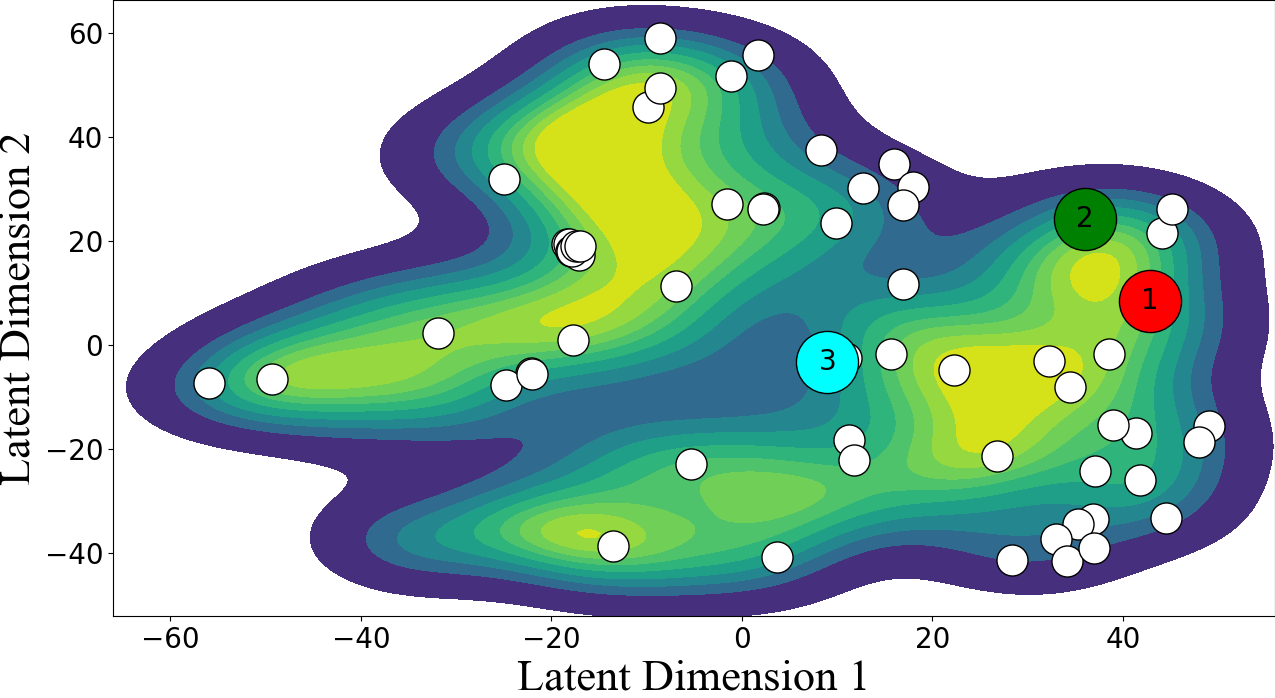
\includegraphics[width=\columnwidth]{chp_sogp/figures/TSNE_task4_kde_p30.png}
			\caption{Reservoir E}
		\end{subfigure}
		\hspace{0.05\columnwidth} % Reduced space between columns
		\begin{subfigure}[t]{0.4\columnwidth}
			\centering
			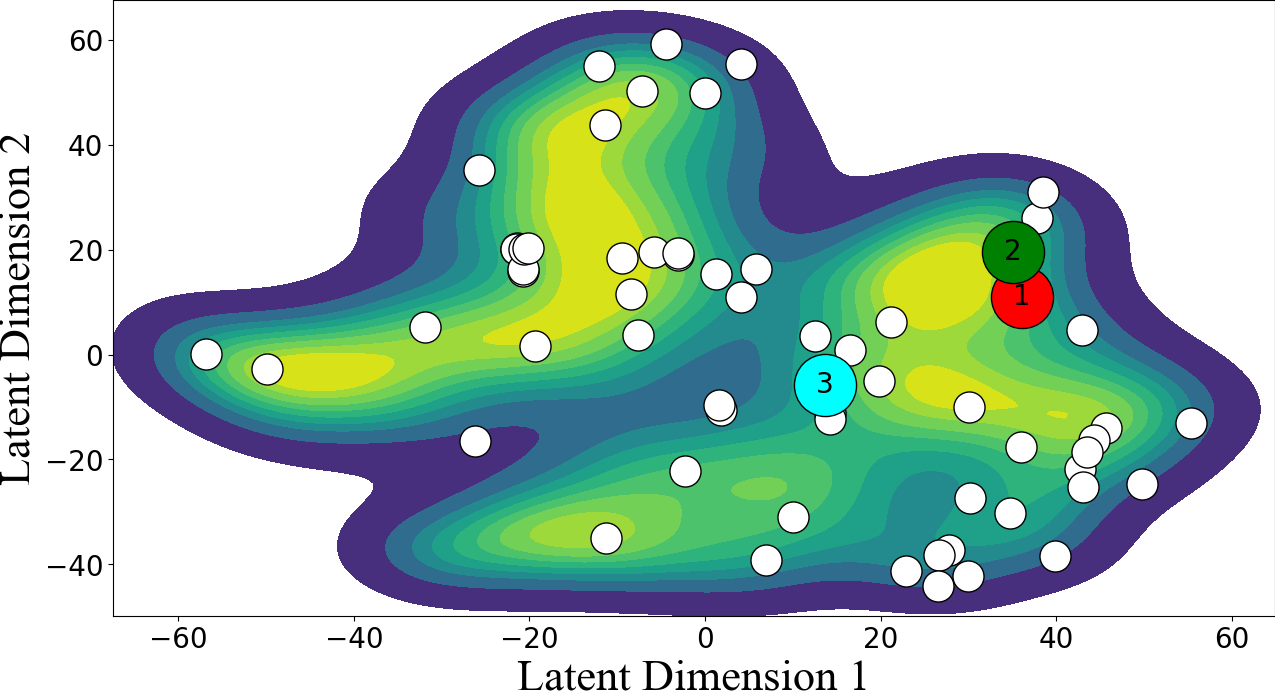
\includegraphics[width=\columnwidth]{chp_sogp/figures/TSNE_task8_kde_p30.png}
			\caption{Reservoir I}
		\end{subfigure}
		
%		\vspace{-0.2em} % Space between rows
		
		\begin{subfigure}[t]{0.4\columnwidth}
			\centering
			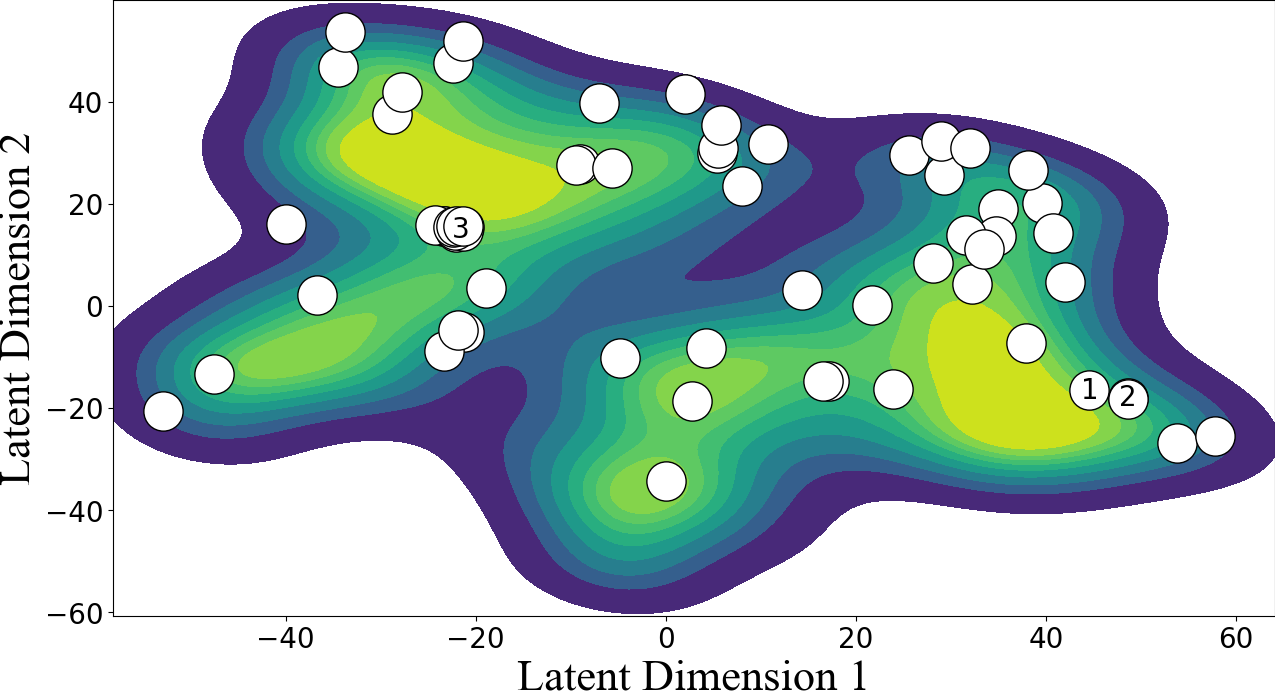
\includegraphics[width=\columnwidth]{chp_sogp/figures/TSNE_task11_kde_p30.png}
			\caption{Reservoir L}
		\end{subfigure}
		\hspace{0.05\columnwidth} % Reduced space between columns
		\begin{subfigure}[t]{0.4\columnwidth}
			\centering
			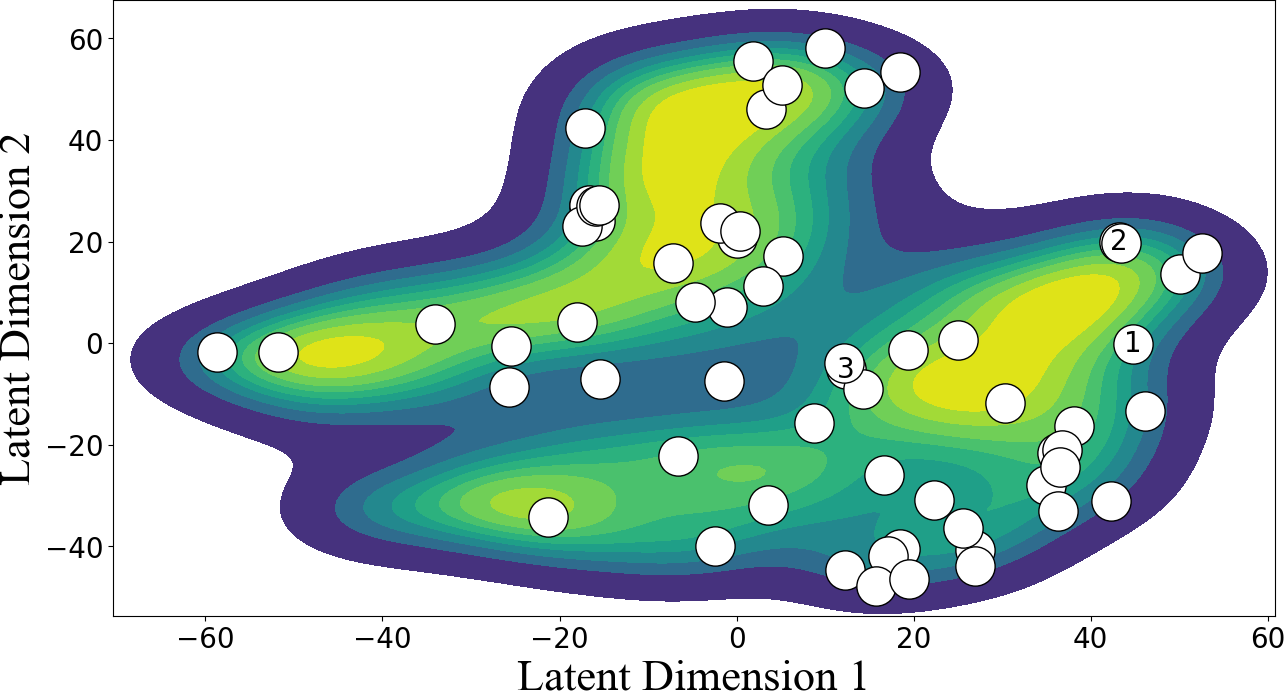
\includegraphics[width=\columnwidth]{chp_sogp/figures/TSNE_task20_kde_p30.png}
			\caption{Reservoir U}
		\end{subfigure}
		
		\vspace{-1.5em} % Space between the figures and the caption
	\end{figure}
	\begin{block}{}
	 The shared inducing points allow for the capturing of task-wise, and global information about the streamflow dynamics.
	\end{block}
\end{frame}


\subsubsection{Performance Analysis}


\begin{frame}{Models Forecasting}
	\centering
	\begin{figure}[htbp]
		\tiny
		\setlength\figurewidth{0.55\columnwidth} 
		\setlength\figureheight{0.5\columnwidth}
		
		\subfloat[$A$.]{% This file was created with tikzplotlib v0.10.1.
\begin{tikzpicture}

\definecolor{darkgray176}{RGB}{176,176,176}
\definecolor{goldenrod1911910}{RGB}{191,191,0}
\definecolor{green01270}{RGB}{0,127,0}
\definecolor{steelblue31119180}{RGB}{31,119,180}
\definecolor{lightgray204}{RGB}{204,204,204}
\definecolor{steelblue76114176}{RGB}{76,114,176}

\begin{axis}[
	width=\figurewidth,
	height=\figureheight,
	axis background/.style={fill=background_color},
	axis line style={white},
	tick align=inside,
	tick pos=left,
	ylabel={Contributions (kWh)},
	ylabel style={font=\tiny},
	x grid style={white},
	xmajorgrids,
	xmin=50, xmax=200,
	xtick style={color=black},
	y grid style={white},
	ymajorgrids,
	ymin=-3414130.1187411, ymax=12497779.277438,
	ytick style={color=black},
	ytick={-4000000,-2000000,0,2000000,4000000,6000000,8000000,10000000,12000000,14000000},
	yticklabels={\ensuremath{-}\tiny0.4,\ensuremath{-}\tiny0.2,\tiny0.0,\tiny0.2,\tiny0.4,\tiny0.6,\tiny0.8,\tiny1.0,\tiny1.2,\tiny1.4},
	tick label style={font=\tiny},  % For all tick labels
	legend columns=6, 
	legend style={
		nodes={scale=0.8, transform shape},
		font=\tiny,
		fill opacity=0.8,
		draw opacity=1,
		text opacity=1,
		at={(0.03,0.97)},
		anchor=north west,
		legend pos=north east,
		draw=lightgray204,
		fill=background_color
	},
]

\path [draw=blue, fill=blue, opacity=0.5]
(axis cs:0,8358734.9454699)
--(axis cs:0,2266980.59308182)
--(axis cs:1,2500001.54965498)
--(axis cs:2,2820173.30462753)
--(axis cs:3,2415130.35524611)
--(axis cs:4,2278827.62176907)
--(axis cs:5,2800080.67146894)
--(axis cs:6,2522735.91826576)
--(axis cs:7,2327115.22470213)
--(axis cs:8,1733100.31528789)
--(axis cs:9,2238909.43945783)
--(axis cs:10,1588035.67664878)
--(axis cs:11,1417358.47856748)
--(axis cs:12,1115298.76632328)
--(axis cs:13,3908825.52055853)
--(axis cs:14,3900131.47830728)
--(axis cs:15,2404535.30116041)
--(axis cs:16,155708.276391005)
--(axis cs:17,2546118.45607269)
--(axis cs:18,2497686.88060658)
--(axis cs:19,2224946.32585587)
--(axis cs:20,3528522.20106472)
--(axis cs:21,2993876.15193917)
--(axis cs:22,3512549.70941467)
--(axis cs:23,2491781.3003113)
--(axis cs:24,2328855.36877622)
--(axis cs:25,1586151.8126521)
--(axis cs:26,1631755.11754632)
--(axis cs:27,1304258.53410548)
--(axis cs:28,1440299.45566472)
--(axis cs:29,2524334.93887751)
--(axis cs:30,1469131.98383735)
--(axis cs:31,844807.886388455)
--(axis cs:32,1306990.45454863)
--(axis cs:33,1656600.4465597)
--(axis cs:34,1108728.6401974)
--(axis cs:35,1291186.74278974)
--(axis cs:36,1264438.19468078)
--(axis cs:37,3058834.81191941)
--(axis cs:38,3164334.38303838)
--(axis cs:39,2162251.43842642)
--(axis cs:40,2410788.57450276)
--(axis cs:41,1847879.46029119)
--(axis cs:42,3957465.21832349)
--(axis cs:43,2602714.55220306)
--(axis cs:44,1722471.05480101)
--(axis cs:45,3241330.05557888)
--(axis cs:46,3288785.66842647)
--(axis cs:47,2601220.79107986)
--(axis cs:48,2394130.4063376)
--(axis cs:49,1607416.13500269)
--(axis cs:50,3800571.8097075)
--(axis cs:51,1769959.66139186)
--(axis cs:52,3592891.04255399)
--(axis cs:53,2577387.46122187)
--(axis cs:54,2068056.39577527)
--(axis cs:55,2024187.16530619)
--(axis cs:56,2168232.03394953)
--(axis cs:57,4219749.91708765)
--(axis cs:58,2321099.19867304)
--(axis cs:59,1852980.63126997)
--(axis cs:60,1666742.29949185)
--(axis cs:61,1700757.83380629)
--(axis cs:62,1900526.36246136)
--(axis cs:63,1784170.84665271)
--(axis cs:64,2525056.64066475)
--(axis cs:65,1561832.5090252)
--(axis cs:66,1053349.26543152)
--(axis cs:67,414485.164985116)
--(axis cs:68,298119.463266004)
--(axis cs:69,81439.3687783941)
--(axis cs:70,-7820.22808993002)
--(axis cs:71,335716.133777275)
--(axis cs:72,4334340.95105938)
--(axis cs:73,1975368.907392)
--(axis cs:74,1288753.12099354)
--(axis cs:75,916344.071282642)
--(axis cs:76,614142.251991577)
--(axis cs:77,1010700.66828775)
--(axis cs:78,461598.17653731)
--(axis cs:79,494501.27675118)
--(axis cs:80,33830.2601246634)
--(axis cs:81,-125567.992846652)
--(axis cs:82,2292069.20046795)
--(axis cs:83,741536.54416309)
--(axis cs:84,919260.944394582)
--(axis cs:85,1658148.94372008)
--(axis cs:86,2302628.50777294)
--(axis cs:87,734480.659289974)
--(axis cs:88,1151364.96245121)
--(axis cs:89,1949088.1892057)
--(axis cs:90,1469898.3748664)
--(axis cs:91,1012199.53992729)
--(axis cs:92,506558.173343586)
--(axis cs:93,337040.472277472)
--(axis cs:94,276181.641666047)
--(axis cs:95,484026.183094725)
--(axis cs:96,53265.2106184359)
--(axis cs:97,979068.968634035)
--(axis cs:98,1723205.76503754)
--(axis cs:99,1479334.21275908)
--(axis cs:100,583871.637923067)
--(axis cs:101,634389.317676129)
--(axis cs:102,215739.931366092)
--(axis cs:103,461739.586981704)
--(axis cs:104,328907.277535586)
--(axis cs:105,-450025.291912541)
--(axis cs:106,-339424.825349538)
--(axis cs:107,859192.193391122)
--(axis cs:108,801036.768157851)
--(axis cs:109,879276.165044384)
--(axis cs:110,880185.232878993)
--(axis cs:111,83383.2972105495)
--(axis cs:112,485151.834711212)
--(axis cs:113,227653.60131191)
--(axis cs:114,810008.874069124)
--(axis cs:115,2435962.86066402)
--(axis cs:116,1538554.12054827)
--(axis cs:117,1131211.72805989)
--(axis cs:118,1356469.14897479)
--(axis cs:119,1207688.63023351)
--(axis cs:120,1552624.63758814)
--(axis cs:121,750359.686908945)
--(axis cs:122,834920.723187054)
--(axis cs:123,697240.26438279)
--(axis cs:124,2102986.1760763)
--(axis cs:125,1996251.22333412)
--(axis cs:126,1756514.14866896)
--(axis cs:127,2360006.57300085)
--(axis cs:128,1993913.19972267)
--(axis cs:129,2157217.91113449)
--(axis cs:130,2316694.30307414)
--(axis cs:131,2394260.09821298)
--(axis cs:132,1848239.17522981)
--(axis cs:133,1767530.89193186)
--(axis cs:134,1540891.21368726)
--(axis cs:135,1462010.18522907)
--(axis cs:136,861297.122579759)
--(axis cs:137,499864.711641925)
--(axis cs:138,-25725.608807263)
--(axis cs:139,-406884.282031849)
--(axis cs:140,-145638.354157871)
--(axis cs:141,134462.892064548)
--(axis cs:142,1348217.08221783)
--(axis cs:143,1479156.2743899)
--(axis cs:144,409275.546300376)
--(axis cs:145,1753441.01561209)
--(axis cs:146,997709.586344555)
--(axis cs:147,570250.159693988)
--(axis cs:148,2432273.85850153)
--(axis cs:149,1534298.14284645)
--(axis cs:150,1577962.02326722)
--(axis cs:151,-574621.177977669)
--(axis cs:152,-183460.994656229)
--(axis cs:153,-261513.429322622)
--(axis cs:154,267649.411942101)
--(axis cs:155,426525.009177709)
--(axis cs:156,570794.146962562)
--(axis cs:157,515871.19444223)
--(axis cs:158,1517382.94619805)
--(axis cs:159,666457.620843957)
--(axis cs:160,1079511.29250439)
--(axis cs:161,607435.347219682)
--(axis cs:162,358485.083181219)
--(axis cs:163,500307.141995887)
--(axis cs:164,487256.966723348)
--(axis cs:165,336996.194720265)
--(axis cs:166,746804.763099345)
--(axis cs:167,1639140.8386245)
--(axis cs:168,2086703.60388984)
--(axis cs:169,2082296.8180802)
--(axis cs:170,2421274.40362573)
--(axis cs:171,2743522.38725703)
--(axis cs:172,3276952.43104429)
--(axis cs:173,1893201.51116063)
--(axis cs:174,1888307.694171)
--(axis cs:175,2564733.61844642)
--(axis cs:176,3201720.08254982)
--(axis cs:177,3383492.24133263)
--(axis cs:178,3247965.71739236)
--(axis cs:179,1653295.63050552)
--(axis cs:180,1420123.69970278)
--(axis cs:181,1321184.89725323)
--(axis cs:182,840604.350411191)
--(axis cs:183,1069709.64984309)
--(axis cs:184,1605780.92757281)
--(axis cs:185,1461822.51297478)
--(axis cs:186,1760629.58786419)
--(axis cs:187,1684856.02697393)
--(axis cs:188,2869595.72832046)
--(axis cs:189,2112473.41992301)
--(axis cs:190,1601863.24076729)
--(axis cs:191,1992571.96940611)
--(axis cs:192,848324.710534492)
--(axis cs:193,-34180.7473299894)
--(axis cs:194,242736.46683395)
--(axis cs:195,320180.542585816)
--(axis cs:196,475112.983168926)
--(axis cs:197,1087350.75172669)
--(axis cs:198,3160250.31426845)
--(axis cs:199,2382899.974148)
--(axis cs:200,1682140.94545173)
--(axis cs:201,1192912.30192668)
--(axis cs:202,2443137.21793836)
--(axis cs:203,3056127.80714893)
--(axis cs:204,3464478.21770381)
--(axis cs:205,1593099.80141614)
--(axis cs:206,2065889.93122398)
--(axis cs:207,1682920.59535471)
--(axis cs:208,3106973.91932809)
--(axis cs:209,2797191.95707892)
--(axis cs:210,2775364.23799069)
--(axis cs:211,1089991.35094045)
--(axis cs:212,1367380.11977648)
--(axis cs:213,820132.807942717)
--(axis cs:214,1395607.06963896)
--(axis cs:215,1597109.15916967)
--(axis cs:216,2324573.18023901)
--(axis cs:217,944706.71099841)
--(axis cs:218,448713.343418519)
--(axis cs:219,-64693.0358876893)
--(axis cs:220,-29204.8480632002)
--(axis cs:221,240341.094173773)
--(axis cs:222,-281918.987639748)
--(axis cs:223,782429.004471717)
--(axis cs:224,521047.354232991)
--(axis cs:225,2345194.14055737)
--(axis cs:226,1368132.63085664)
--(axis cs:227,1230991.94258766)
--(axis cs:228,611057.273470148)
--(axis cs:229,77204.2095062481)
--(axis cs:230,-703629.858866641)
--(axis cs:231,-568034.528975812)
--(axis cs:232,-618345.175514996)
--(axis cs:233,-261129.287755128)
--(axis cs:234,-330004.860701131)
--(axis cs:235,-629314.936891818)
--(axis cs:236,-849909.293658883)
--(axis cs:237,-862056.450460804)
--(axis cs:238,-1491479.62577631)
--(axis cs:239,-1205160.6270297)
--(axis cs:240,-1236502.82817937)
--(axis cs:241,-421657.747989412)
--(axis cs:242,-1423787.05278457)
--(axis cs:243,-1727855.67463412)
--(axis cs:244,-1598521.89810558)
--(axis cs:245,-1384421.17327104)
--(axis cs:246,-1647104.77201385)
--(axis cs:247,-738046.085897258)
--(axis cs:248,-1504644.1046588)
--(axis cs:249,-1411386.36475813)
--(axis cs:250,-1403729.74361189)
--(axis cs:251,-1753899.81215703)
--(axis cs:252,-1549664.37286907)
--(axis cs:253,-1527701.31484671)
--(axis cs:254,-1362069.49284841)
--(axis cs:255,-1150810.85721608)
--(axis cs:256,-1263813.85555845)
--(axis cs:257,-668997.20244717)
--(axis cs:258,-1376281.03749657)
--(axis cs:259,-1087811.89019368)
--(axis cs:260,-1792309.2243679)
--(axis cs:261,-1917762.69837502)
--(axis cs:262,-1805955.64995552)
--(axis cs:263,-2260570.46921006)
--(axis cs:264,-1737120.45891163)
--(axis cs:265,-2032940.50447617)
--(axis cs:266,-1994001.01461112)
--(axis cs:267,-2028487.78775041)
--(axis cs:268,-1876425.76046569)
--(axis cs:269,-1291257.29209179)
--(axis cs:270,-648339.275730376)
--(axis cs:271,-1414311.32024024)
--(axis cs:272,-1754111.68023554)
--(axis cs:273,15785.7347802464)
--(axis cs:274,-346974.721788103)
--(axis cs:275,1295901.9458233)
--(axis cs:276,1280049.25219146)
--(axis cs:277,3091769.23677594)
--(axis cs:278,478672.307735468)
--(axis cs:279,395121.886578801)
--(axis cs:280,1636651.53361617)
--(axis cs:281,2575452.65146408)
--(axis cs:282,1469880.05512509)
--(axis cs:283,409829.911913471)
--(axis cs:284,631886.887580078)
--(axis cs:285,1893459.51588553)
--(axis cs:286,1368747.82714392)
--(axis cs:287,2407299.04277756)
--(axis cs:288,1390231.15819764)
--(axis cs:289,845028.71176875)
--(axis cs:290,1078146.57392484)
--(axis cs:291,972736.009060407)
--(axis cs:292,2992084.14802539)
--(axis cs:293,1966899.24784066)
--(axis cs:294,1582957.82595676)
--(axis cs:295,840697.009995176)
--(axis cs:296,570127.448758581)
--(axis cs:297,397552.276297163)
--(axis cs:298,1586229.90271889)
--(axis cs:299,938523.394328011)
--(axis cs:300,1637042.45551103)
--(axis cs:301,914360.994266017)
--(axis cs:302,102882.752574615)
--(axis cs:303,-393332.32100678)
--(axis cs:304,-424121.266243435)
--(axis cs:305,-289170.393837035)
--(axis cs:306,238565.073043851)
--(axis cs:307,791733.052337766)
--(axis cs:308,-38829.974295829)
--(axis cs:309,-545955.758686787)
--(axis cs:310,-586167.017135648)
--(axis cs:311,-442755.470135127)
--(axis cs:312,-531960.643466798)
--(axis cs:313,676124.109715074)
--(axis cs:314,-482649.734332843)
--(axis cs:315,1038283.73788468)
--(axis cs:316,205623.613565952)
--(axis cs:317,-381544.513242999)
--(axis cs:318,-406899.261562913)
--(axis cs:319,-284535.667012632)
--(axis cs:320,-286305.34626342)
--(axis cs:321,-346316.139303518)
--(axis cs:322,1040410.23285963)
--(axis cs:323,589404.961613129)
--(axis cs:324,707913.640332953)
--(axis cs:325,771388.936261653)
--(axis cs:326,595756.507183571)
--(axis cs:327,1054199.78227143)
--(axis cs:328,-305803.963151428)
--(axis cs:329,-593837.554806351)
--(axis cs:330,782481.948940561)
--(axis cs:331,1365746.26804607)
--(axis cs:332,958640.839148703)
--(axis cs:333,2339132.88508022)
--(axis cs:334,1050245.55835239)
--(axis cs:335,1221166.38615646)
--(axis cs:336,1195115.99955142)
--(axis cs:337,1096576.70209503)
--(axis cs:338,124977.524378125)
--(axis cs:339,965167.867562695)
--(axis cs:340,946780.992962114)
--(axis cs:341,739002.977938325)
--(axis cs:342,181450.554034516)
--(axis cs:343,139619.759726186)
--(axis cs:344,1085985.43091181)
--(axis cs:345,1146123.74095834)
--(axis cs:346,812329.486530669)
--(axis cs:347,641654.079815982)
--(axis cs:348,1217153.43036141)
--(axis cs:349,2473295.74536918)
--(axis cs:350,1314982.34765331)
--(axis cs:351,1772772.7666509)
--(axis cs:352,1215612.15422667)
--(axis cs:353,2146959.95908049)
--(axis cs:354,1837210.0040028)
--(axis cs:355,2033462.32888738)
--(axis cs:356,1980010.05607892)
--(axis cs:357,3039414.06621217)
--(axis cs:358,1863881.29906812)
--(axis cs:359,1531237.77681536)
--(axis cs:360,1207145.45452158)
--(axis cs:361,1224623.29228109)
--(axis cs:362,1742385.07182669)
--(axis cs:363,2904790.43576386)
--(axis cs:364,2547719.0813286)
--(axis cs:365,2854339.44720298)
--(axis cs:366,1257049.88256602)
--(axis cs:367,1870755.24321553)
--(axis cs:368,2614474.04894225)
--(axis cs:369,1588831.44143394)
--(axis cs:370,2360313.84061642)
--(axis cs:371,2401318.17182898)
--(axis cs:372,3064833.4140743)
--(axis cs:373,3192050.70963895)
--(axis cs:374,2663007.27200022)
--(axis cs:375,3709118.23830217)
--(axis cs:376,2335728.38327879)
--(axis cs:377,4025739.01063027)
--(axis cs:378,4055408.83132899)
--(axis cs:379,2960992.68942342)
--(axis cs:380,2657390.42843395)
--(axis cs:381,2722234.42908046)
--(axis cs:382,3103809.54765794)
--(axis cs:383,3272887.22177995)
--(axis cs:384,2741714.33565594)
--(axis cs:385,3707114.31719387)
--(axis cs:386,3515979.43874086)
--(axis cs:387,2687537.20342327)
--(axis cs:388,2840202.86134352)
--(axis cs:389,3053290.7891614)
--(axis cs:390,2624280.63959711)
--(axis cs:391,1996525.2894387)
--(axis cs:392,3987152.74982535)
--(axis cs:393,3488735.45628922)
--(axis cs:394,4859209.60018155)
--(axis cs:395,3785810.63864612)
--(axis cs:396,2651825.09161797)
--(axis cs:397,2342689.32647771)
--(axis cs:398,1724308.38006152)
--(axis cs:399,3116503.58527372)
--(axis cs:400,2713962.51998371)
--(axis cs:401,2924991.8355552)
--(axis cs:402,1759784.98522933)
--(axis cs:403,2663118.2481602)
--(axis cs:404,4544813.79217867)
--(axis cs:405,5064879.7229684)
--(axis cs:406,3647294.34128199)
--(axis cs:407,2477553.36206289)
--(axis cs:408,2357641.3363899)
--(axis cs:409,3691593.57461331)
--(axis cs:410,2712420.65312779)
--(axis cs:411,2180599.51772762)
--(axis cs:412,3085656.53750853)
--(axis cs:413,2915976.19105762)
--(axis cs:414,3075394.13093566)
--(axis cs:415,3303878.67127666)
--(axis cs:416,2288488.00111913)
--(axis cs:417,1884126.24464031)
--(axis cs:418,1562775.86596284)
--(axis cs:419,1670034.05930531)
--(axis cs:420,1330120.0918032)
--(axis cs:421,1245506.03135283)
--(axis cs:422,1139180.17608696)
--(axis cs:423,1716689.00137541)
--(axis cs:424,1127174.99347224)
--(axis cs:425,920644.833256553)
--(axis cs:426,833019.426799105)
--(axis cs:427,977829.022656063)
--(axis cs:428,573895.003956363)
--(axis cs:429,304425.050964801)
--(axis cs:430,385634.028432807)
--(axis cs:431,3170498.39166676)
--(axis cs:432,1269443.10069475)
--(axis cs:433,582683.241494185)
--(axis cs:434,338342.607890409)
--(axis cs:435,198134.636922647)
--(axis cs:436,3700128.99467785)
--(axis cs:437,3708934.5229381)
--(axis cs:438,2126149.2257448)
--(axis cs:439,3653330.29513892)
--(axis cs:440,2375245.67171627)
--(axis cs:440,8272115.97564292)
--(axis cs:440,8272115.97564292)
--(axis cs:439,10011577.5456571)
--(axis cs:438,7997611.41757856)
--(axis cs:437,9635565.99844665)
--(axis cs:436,9607828.31427181)
--(axis cs:435,6072861.77476716)
--(axis cs:434,6212873.20124285)
--(axis cs:433,6452280.79079365)
--(axis cs:432,7149477.70611468)
--(axis cs:431,9063394.31624093)
--(axis cs:430,6283774.64694488)
--(axis cs:429,6196312.25641046)
--(axis cs:428,6616585.42512907)
--(axis cs:427,6906795.03319433)
--(axis cs:426,6763781.61119613)
--(axis cs:425,7012796.19856471)
--(axis cs:424,7089689.32194692)
--(axis cs:423,7656594.18475407)
--(axis cs:422,7095689.9374345)
--(axis cs:421,7289410.08378023)
--(axis cs:420,7505021.90638861)
--(axis cs:419,7713792.59164026)
--(axis cs:418,7511894.8093766)
--(axis cs:417,7947574.99178663)
--(axis cs:416,8241270.69192941)
--(axis cs:415,9272062.72279752)
--(axis cs:414,9003539.46431187)
--(axis cs:413,8846613.44772675)
--(axis cs:412,9105367.22263592)
--(axis cs:411,8079776.77631247)
--(axis cs:410,8600197.55973165)
--(axis cs:409,9684244.9945811)
--(axis cs:408,8227475.4132527)
--(axis cs:407,8351959.65928155)
--(axis cs:406,9556521.83074564)
--(axis cs:405,11088718.651684)
--(axis cs:404,10562655.5164873)
--(axis cs:403,8677451.54084561)
--(axis cs:402,7724399.75366388)
--(axis cs:401,8900148.4912878)
--(axis cs:400,8619427.20856482)
--(axis cs:399,9023644.62626584)
--(axis cs:398,7654322.89644653)
--(axis cs:397,8325906.4041908)
--(axis cs:396,8854878.21402704)
--(axis cs:395,10134240.9070042)
--(axis cs:394,10942794.0012594)
--(axis cs:393,9412306.42744924)
--(axis cs:392,9890440.27644084)
--(axis cs:391,7862314.42334116)
--(axis cs:390,8539608.8276385)
--(axis cs:389,8943656.49523974)
--(axis cs:388,8749942.91793317)
--(axis cs:387,8705300.56734983)
--(axis cs:386,9451385.92980784)
--(axis cs:385,9661638.45024246)
--(axis cs:384,8800115.49330164)
--(axis cs:383,9329078.99326154)
--(axis cs:382,9119536.39494003)
--(axis cs:381,8711040.05201311)
--(axis cs:380,9049290.99227471)
--(axis cs:379,9504148.53201147)
--(axis cs:378,10410231.6107597)
--(axis cs:377,10326557.3212269)
--(axis cs:376,8728582.683576)
--(axis cs:375,9673920.17516636)
--(axis cs:374,8634933.11425413)
--(axis cs:373,9157477.21893432)
--(axis cs:372,9157929.60738453)
--(axis cs:371,8326286.22268122)
--(axis cs:370,8242256.81424885)
--(axis cs:369,7508145.32098696)
--(axis cs:368,8546925.55539232)
--(axis cs:367,7878369.78688992)
--(axis cs:366,7749147.7691826)
--(axis cs:365,8777805.04685025)
--(axis cs:364,8621207.45742553)
--(axis cs:363,8936822.6694143)
--(axis cs:362,8026606.42024076)
--(axis cs:361,7196783.10732654)
--(axis cs:360,7413401.58474042)
--(axis cs:359,7555906.77588987)
--(axis cs:358,8088401.43404874)
--(axis cs:357,9679920.01725985)
--(axis cs:356,8076758.88553188)
--(axis cs:355,8052209.41518265)
--(axis cs:354,7933664.42316086)
--(axis cs:353,8492570.42424654)
--(axis cs:352,7308779.19156219)
--(axis cs:351,7818817.95504795)
--(axis cs:350,7573739.38620749)
--(axis cs:349,8797907.06987265)
--(axis cs:348,7375941.65053311)
--(axis cs:347,6569846.35313213)
--(axis cs:346,6743196.52320619)
--(axis cs:345,7044621.54291345)
--(axis cs:344,7092701.77476335)
--(axis cs:343,6136173.89898583)
--(axis cs:342,6344575.61516148)
--(axis cs:341,6779463.28788147)
--(axis cs:340,6860105.47907654)
--(axis cs:339,6944443.82978215)
--(axis cs:338,6237386.42674522)
--(axis cs:337,7133470.37297508)
--(axis cs:336,7418021.26036287)
--(axis cs:335,7132481.80986207)
--(axis cs:334,6943400.89190936)
--(axis cs:333,8351541.70390249)
--(axis cs:332,6994699.02333084)
--(axis cs:331,7366236.27538514)
--(axis cs:330,6736401.87984606)
--(axis cs:329,5729913.61972009)
--(axis cs:328,6152138.0355138)
--(axis cs:327,7091179.723979)
--(axis cs:326,6587905.42111292)
--(axis cs:325,6741081.92349823)
--(axis cs:324,6927522.95220145)
--(axis cs:323,6732134.31011498)
--(axis cs:322,7414879.48424147)
--(axis cs:321,5646266.81566105)
--(axis cs:320,5639928.66468998)
--(axis cs:319,5611793.89013555)
--(axis cs:318,5520410.31099636)
--(axis cs:317,5557630.12102689)
--(axis cs:316,6317348.65003779)
--(axis cs:315,8133806.0487823)
--(axis cs:314,6271361.26806303)
--(axis cs:313,6926779.59231562)
--(axis cs:312,5351487.17626322)
--(axis cs:311,5487382.36968934)
--(axis cs:310,5293847.53066585)
--(axis cs:309,5313036.47539066)
--(axis cs:308,5836358.77445582)
--(axis cs:307,6806428.95975679)
--(axis cs:306,6145055.03764359)
--(axis cs:305,5597596.29577675)
--(axis cs:304,5615029.20658272)
--(axis cs:303,5746438.19449132)
--(axis cs:302,6044624.93079489)
--(axis cs:301,6883756.24313143)
--(axis cs:300,7717297.41396964)
--(axis cs:299,6999180.00143638)
--(axis cs:298,7722016.09685706)
--(axis cs:297,6500962.58968753)
--(axis cs:296,6439857.44289134)
--(axis cs:295,6708598.62648087)
--(axis cs:294,7544073.9674112)
--(axis cs:293,8101619.38663902)
--(axis cs:292,9116088.93195463)
--(axis cs:291,6989022.07507434)
--(axis cs:290,6970124.22981287)
--(axis cs:289,7056445.31115333)
--(axis cs:288,7295821.7252935)
--(axis cs:287,8376488.11238208)
--(axis cs:286,7578421.4232308)
--(axis cs:285,8046576.21229546)
--(axis cs:284,7212922.64090839)
--(axis cs:283,6521406.92841331)
--(axis cs:282,7554490.42794916)
--(axis cs:281,8681908.70211522)
--(axis cs:280,7858043.03039205)
--(axis cs:279,6922764.17147553)
--(axis cs:278,6880386.67496839)
--(axis cs:277,9146553.78321283)
--(axis cs:276,7379428.98116728)
--(axis cs:275,7513575.53765563)
--(axis cs:274,5741060.86128361)
--(axis cs:273,6170870.39527822)
--(axis cs:272,4412738.07280879)
--(axis cs:271,5125181.63389964)
--(axis cs:270,5279902.76289232)
--(axis cs:269,4601444.70584617)
--(axis cs:268,4004144.58825829)
--(axis cs:267,3867664.14440554)
--(axis cs:266,3918913.50021261)
--(axis cs:265,3901956.96393358)
--(axis cs:264,4429298.28023224)
--(axis cs:263,3685876.01529592)
--(axis cs:262,4107167.51973562)
--(axis cs:261,4092723.1457314)
--(axis cs:260,4970792.8097317)
--(axis cs:259,4907549.33909286)
--(axis cs:258,4562806.88204193)
--(axis cs:257,5564992.31940384)
--(axis cs:256,4742276.74049143)
--(axis cs:255,4977378.99761699)
--(axis cs:254,4934040.50236445)
--(axis cs:253,4875146.15793132)
--(axis cs:252,4849843.12505433)
--(axis cs:251,4591102.05855391)
--(axis cs:250,4680614.08481247)
--(axis cs:249,4806759.63655051)
--(axis cs:248,5398519.23058963)
--(axis cs:247,5924235.62056438)
--(axis cs:246,4577806.77403004)
--(axis cs:245,4562165.87791714)
--(axis cs:244,4419361.76158695)
--(axis cs:243,4519559.84972538)
--(axis cs:242,4903736.64106637)
--(axis cs:241,6474664.50268905)
--(axis cs:240,5034204.73774535)
--(axis cs:239,5203836.55271089)
--(axis cs:238,4889401.78115006)
--(axis cs:237,5028271.6617677)
--(axis cs:236,5030147.92350487)
--(axis cs:235,5249275.18224642)
--(axis cs:234,5540223.699851)
--(axis cs:233,5608686.81977924)
--(axis cs:232,5668616.25525784)
--(axis cs:231,5371440.13637239)
--(axis cs:230,5246016.17185683)
--(axis cs:229,6114481.1296214)
--(axis cs:228,6592394.04485644)
--(axis cs:227,7233892.55599388)
--(axis cs:226,7560745.16767292)
--(axis cs:225,8311358.80833407)
--(axis cs:224,7495803.994909)
--(axis cs:223,6878220.36672014)
--(axis cs:222,6160229.64507523)
--(axis cs:221,7318835.36975051)
--(axis cs:220,7246663.17516622)
--(axis cs:219,6615836.61209439)
--(axis cs:218,6749113.88839668)
--(axis cs:217,7107473.99710223)
--(axis cs:216,8555535.72940454)
--(axis cs:215,8367306.12768181)
--(axis cs:214,8095423.00720392)
--(axis cs:213,7694157.98714085)
--(axis cs:212,8323090.08105852)
--(axis cs:211,7995439.59566517)
--(axis cs:210,9045449.95771611)
--(axis cs:209,9564570.78842258)
--(axis cs:208,9821419.46295298)
--(axis cs:207,7837769.33742558)
--(axis cs:206,8255574.25607588)
--(axis cs:205,7849736.53431507)
--(axis cs:204,9576660.33798847)
--(axis cs:203,9368591.47472401)
--(axis cs:202,9165616.33649763)
--(axis cs:201,8390043.92014571)
--(axis cs:200,8607782.67335589)
--(axis cs:199,8799351.17919425)
--(axis cs:198,9357307.81325061)
--(axis cs:197,7483283.09942182)
--(axis cs:196,6683454.5725114)
--(axis cs:195,7053163.66442116)
--(axis cs:194,7565404.86683807)
--(axis cs:193,6200732.26408663)
--(axis cs:192,7171495.15083943)
--(axis cs:191,8203105.65223896)
--(axis cs:190,7498392.46651707)
--(axis cs:189,8076362.84351501)
--(axis cs:188,9058808.51068171)
--(axis cs:187,8821475.6751613)
--(axis cs:186,8751212.73423382)
--(axis cs:185,8118458.38378642)
--(axis cs:184,8124343.62316064)
--(axis cs:183,7007270.76272865)
--(axis cs:182,6940343.87525926)
--(axis cs:181,7304634.6108532)
--(axis cs:180,7564718.08769193)
--(axis cs:179,8328475.01770524)
--(axis cs:178,9485792.02733359)
--(axis cs:177,9689734.59750967)
--(axis cs:176,9450465.06717683)
--(axis cs:175,8948079.59175623)
--(axis cs:174,8405988.85831612)
--(axis cs:173,8741083.26570942)
--(axis cs:172,9968137.23215174)
--(axis cs:171,9126666.41570682)
--(axis cs:170,8496109.73289019)
--(axis cs:169,8829265.88352662)
--(axis cs:168,8360476.29898034)
--(axis cs:167,7651737.10059532)
--(axis cs:166,6754528.58466087)
--(axis cs:165,6221099.08431227)
--(axis cs:164,6336008.42282694)
--(axis cs:163,6390368.43425088)
--(axis cs:162,6606684.21313195)
--(axis cs:161,6463712.2109056)
--(axis cs:160,6971719.21072575)
--(axis cs:159,6527237.92416448)
--(axis cs:158,7448595.25540128)
--(axis cs:157,6552109.10429121)
--(axis cs:156,6876578.59679644)
--(axis cs:155,6361114.3912048)
--(axis cs:154,6338968.35592609)
--(axis cs:153,5743938.08214018)
--(axis cs:152,5713168.05937878)
--(axis cs:151,6009137.88882062)
--(axis cs:150,7517804.93430203)
--(axis cs:149,7453006.41713491)
--(axis cs:148,8823440.02242871)
--(axis cs:147,6479591.52044145)
--(axis cs:146,6995421.00812897)
--(axis cs:145,8233454.97190743)
--(axis cs:144,6713913.47421679)
--(axis cs:143,7439774.41928997)
--(axis cs:142,7368120.91903883)
--(axis cs:141,6110114.93413916)
--(axis cs:140,5835392.60034468)
--(axis cs:139,5645436.82020181)
--(axis cs:138,6216849.71122078)
--(axis cs:137,6512801.79719511)
--(axis cs:136,6822078.74304201)
--(axis cs:135,7626219.47830896)
--(axis cs:134,7767868.70129548)
--(axis cs:133,7887300.40473132)
--(axis cs:132,8530712.12434376)
--(axis cs:131,8585430.70651424)
--(axis cs:130,8687812.82110287)
--(axis cs:129,8496024.70025284)
--(axis cs:128,8534211.24710132)
--(axis cs:127,8780268.08636291)
--(axis cs:126,8507297.96736859)
--(axis cs:125,8257204.86348395)
--(axis cs:124,8315657.53908073)
--(axis cs:123,7344078.02207404)
--(axis cs:122,6861840.24356864)
--(axis cs:121,7104377.22877023)
--(axis cs:120,7926765.7469317)
--(axis cs:119,7186307.56303116)
--(axis cs:118,7331921.3006784)
--(axis cs:117,7054113.09715032)
--(axis cs:116,8036195.88384113)
--(axis cs:115,8400746.88129105)
--(axis cs:114,6767631.53735761)
--(axis cs:113,6489285.1899857)
--(axis cs:112,6572828.73970546)
--(axis cs:111,6589342.49793673)
--(axis cs:110,7050296.12744666)
--(axis cs:109,6941615.68986246)
--(axis cs:108,6727736.37519017)
--(axis cs:107,7032339.83230106)
--(axis cs:106,5942141.16199991)
--(axis cs:105,5580414.23217365)
--(axis cs:104,6196126.35290635)
--(axis cs:103,6369006.45094391)
--(axis cs:102,6243937.36821829)
--(axis cs:101,6552787.49936702)
--(axis cs:100,6543608.10188798)
--(axis cs:99,7382894.8860172)
--(axis cs:98,7622566.72894418)
--(axis cs:97,6838346.22382169)
--(axis cs:96,5920294.43025754)
--(axis cs:95,6441826.59383301)
--(axis cs:94,6149797.52850492)
--(axis cs:93,6206888.85275809)
--(axis cs:92,6388734.23595245)
--(axis cs:91,6884044.87736475)
--(axis cs:90,7411976.85666203)
--(axis cs:89,7850708.56649312)
--(axis cs:88,7005061.36887078)
--(axis cs:87,6580907.25089671)
--(axis cs:86,8170430.18127629)
--(axis cs:85,7688961.45795676)
--(axis cs:84,6789576.38948332)
--(axis cs:83,6587541.17027693)
--(axis cs:82,8163788.22862993)
--(axis cs:81,5728882.98666019)
--(axis cs:80,5881873.52566259)
--(axis cs:79,6346344.07212325)
--(axis cs:78,6322332.28316718)
--(axis cs:77,6868374.19837788)
--(axis cs:76,6467593.4559952)
--(axis cs:75,6790634.5611246)
--(axis cs:74,7189172.85758338)
--(axis cs:73,7845279.66202889)
--(axis cs:72,10309744.0530896)
--(axis cs:71,6181063.40738308)
--(axis cs:70,5873490.67430435)
--(axis cs:69,5942240.9806898)
--(axis cs:68,6151217.53147982)
--(axis cs:67,6281228.43259183)
--(axis cs:66,6921993.32150405)
--(axis cs:65,7430653.31981543)
--(axis cs:64,8406789.07029833)
--(axis cs:63,7678032.30836992)
--(axis cs:62,7779339.94755391)
--(axis cs:61,7691533.04200607)
--(axis cs:60,8118902.77594928)
--(axis cs:59,7888649.84230029)
--(axis cs:58,8231240.35421631)
--(axis cs:57,10225728.8837369)
--(axis cs:56,8284864.42376014)
--(axis cs:55,8056270.85700612)
--(axis cs:54,8188802.99412978)
--(axis cs:53,8587803.84291661)
--(axis cs:52,9757365.74140004)
--(axis cs:51,7774258.72978544)
--(axis cs:50,9773012.90077685)
--(axis cs:49,7543662.45878557)
--(axis cs:48,8366369.02485663)
--(axis cs:47,8527050.32973806)
--(axis cs:46,9288516.00961098)
--(axis cs:45,9215131.79049679)
--(axis cs:44,8465639.15914963)
--(axis cs:43,8848468.33443262)
--(axis cs:42,9975524.31028236)
--(axis cs:41,7716513.35888516)
--(axis cs:40,8585590.444903)
--(axis cs:39,8046697.65811915)
--(axis cs:38,9061277.56638082)
--(axis cs:37,8959598.76533762)
--(axis cs:36,7171564.90185334)
--(axis cs:35,7145907.04617949)
--(axis cs:34,6965455.88627264)
--(axis cs:33,7617839.5279707)
--(axis cs:32,7159094.12709909)
--(axis cs:31,6700804.58801861)
--(axis cs:30,7343517.78973181)
--(axis cs:29,8431175.26424769)
--(axis cs:28,7330522.14541852)
--(axis cs:27,7225547.45175696)
--(axis cs:26,7537979.7512287)
--(axis cs:25,7488757.26602932)
--(axis cs:24,8242394.44899235)
--(axis cs:23,8379204.91061556)
--(axis cs:22,9441647.08735033)
--(axis cs:21,9266193.03407906)
--(axis cs:20,9728685.25839887)
--(axis cs:19,8322686.81444134)
--(axis cs:18,8687097.44746864)
--(axis cs:17,8804705.0708452)
--(axis cs:16,7481962.56861928)
--(axis cs:15,8359167.58209611)
--(axis cs:14,9917343.03729903)
--(axis cs:13,9901265.5631022)
--(axis cs:12,7058300.0424605)
--(axis cs:11,7300393.23963672)
--(axis cs:10,7631033.41849808)
--(axis cs:9,8404156.88651083)
--(axis cs:8,8227013.51280867)
--(axis cs:7,8862452.77799191)
--(axis cs:6,9114397.94396872)
--(axis cs:5,9233470.8886454)
--(axis cs:4,9147653.1877756)
--(axis cs:3,8830004.51601952)
--(axis cs:2,9353245.08095938)
--(axis cs:1,9366401.36241324)
--(axis cs:0,8358734.9454699)
--cycle;

\path [draw=goldenrod1911910, fill=goldenrod1911910, opacity=0.5]
(axis cs:0,7649611.36140954)
--(axis cs:0,2031353.86694591)
--(axis cs:1,3519778.99023208)
--(axis cs:2,2939647.83093819)
--(axis cs:3,2404739.40901625)
--(axis cs:4,2599711.14663126)
--(axis cs:5,2663728.74643248)
--(axis cs:6,2426379.1016333)
--(axis cs:7,2232546.72630842)
--(axis cs:8,1668469.54697674)
--(axis cs:9,2057827.52360267)
--(axis cs:10,1490958.45797037)
--(axis cs:11,1185100.63458257)
--(axis cs:12,964716.243901049)
--(axis cs:13,3834280.95472574)
--(axis cs:14,4058426.74441934)
--(axis cs:15,2463915.32277849)
--(axis cs:16,1625007.40781802)
--(axis cs:17,2045788.16372025)
--(axis cs:18,2615535.96239301)
--(axis cs:19,2108399.57141996)
--(axis cs:20,4265001.05360169)
--(axis cs:21,3419640.3442961)
--(axis cs:22,3311831.70608119)
--(axis cs:23,2378382.24669818)
--(axis cs:24,2299225.49424298)
--(axis cs:25,1586672.89565133)
--(axis cs:26,1734188.38705589)
--(axis cs:27,1377097.6756055)
--(axis cs:28,1501859.3903355)
--(axis cs:29,2519230.24015983)
--(axis cs:30,1602768.89488034)
--(axis cs:31,994183.893438096)
--(axis cs:32,1383863.25026629)
--(axis cs:33,1846530.28765762)
--(axis cs:34,1239775.97277975)
--(axis cs:35,1394730.10840429)
--(axis cs:36,1388129.72336291)
--(axis cs:37,3212874.42384193)
--(axis cs:38,3250052.05093703)
--(axis cs:39,2212330.83063421)
--(axis cs:40,2988267.81816703)
--(axis cs:41,1940811.17360877)
--(axis cs:42,4501668.5981036)
--(axis cs:43,4362329.57020703)
--(axis cs:44,4774876.89487605)
--(axis cs:45,3761577.41166215)
--(axis cs:46,3833183.17858582)
--(axis cs:47,2941135.19156964)
--(axis cs:48,3050059.16855053)
--(axis cs:49,2065029.89060203)
--(axis cs:50,4500022.86644034)
--(axis cs:51,2272764.7465469)
--(axis cs:52,4794628.18392887)
--(axis cs:53,3185752.31783906)
--(axis cs:54,3393025.53630686)
--(axis cs:55,2763798.96680438)
--(axis cs:56,3090198.52648587)
--(axis cs:57,4515895.54251675)
--(axis cs:58,2597299.22762645)
--(axis cs:59,2047454.01280886)
--(axis cs:60,3077708.1641259)
--(axis cs:61,1923991.90230687)
--(axis cs:62,2023265.34145536)
--(axis cs:63,1945120.18593477)
--(axis cs:64,2671939.69385065)
--(axis cs:65,1712801.45250672)
--(axis cs:66,1257472.62148182)
--(axis cs:67,669374.331022673)
--(axis cs:68,525431.049548327)
--(axis cs:69,354030.832588086)
--(axis cs:70,223072.663671357)
--(axis cs:71,547211.055081147)
--(axis cs:72,4891812.83621656)
--(axis cs:73,1967492.40125675)
--(axis cs:74,1546038.27733403)
--(axis cs:75,995871.714654822)
--(axis cs:76,744308.887271639)
--(axis cs:77,1195718.70252183)
--(axis cs:78,664904.436480089)
--(axis cs:79,635419.536387467)
--(axis cs:80,269721.970536069)
--(axis cs:81,121292.406592703)
--(axis cs:82,2419182.85003434)
--(axis cs:83,818592.975010572)
--(axis cs:84,972004.782306544)
--(axis cs:85,1878727.1436674)
--(axis cs:86,2327387.28519245)
--(axis cs:87,909879.323522354)
--(axis cs:88,1265832.79529863)
--(axis cs:89,2068057.92654706)
--(axis cs:90,1703252.06764654)
--(axis cs:91,1113763.15278355)
--(axis cs:92,543285.504705829)
--(axis cs:93,464062.304703045)
--(axis cs:94,420561.625391634)
--(axis cs:95,970038.564103642)
--(axis cs:96,239762.295294122)
--(axis cs:97,1253147.13821133)
--(axis cs:98,1917151.5980573)
--(axis cs:99,1774552.46575942)
--(axis cs:100,776063.778164456)
--(axis cs:101,813515.709810239)
--(axis cs:102,786952.781699222)
--(axis cs:103,693673.769717739)
--(axis cs:104,561581.60775435)
--(axis cs:105,-9449.11910516536)
--(axis cs:106,140563.902805642)
--(axis cs:107,1390080.20385617)
--(axis cs:108,917707.095869979)
--(axis cs:109,1637776.6105716)
--(axis cs:110,1516861.73686869)
--(axis cs:111,522320.456940449)
--(axis cs:112,791543.269129801)
--(axis cs:113,485495.585377553)
--(axis cs:114,1006838.30867687)
--(axis cs:115,2629796.0113633)
--(axis cs:116,3068871.19888404)
--(axis cs:117,1353594.42178321)
--(axis cs:118,1607003.6062809)
--(axis cs:119,1418412.93529407)
--(axis cs:120,2019398.0635785)
--(axis cs:121,1276219.55230597)
--(axis cs:122,1022015.57819442)
--(axis cs:123,1444372.47035012)
--(axis cs:124,2383625.07692119)
--(axis cs:125,2458447.44376003)
--(axis cs:126,2747159.64731046)
--(axis cs:127,2986996.31238164)
--(axis cs:128,2553268.52467772)
--(axis cs:129,2492825.67459294)
--(axis cs:130,3042842.78513953)
--(axis cs:131,2546061.12872144)
--(axis cs:132,2597984.60251658)
--(axis cs:133,1932673.18498694)
--(axis cs:134,2094101.17897937)
--(axis cs:135,1346176.48957805)
--(axis cs:136,987586.951263016)
--(axis cs:137,728988.962961117)
--(axis cs:138,315617.909551716)
--(axis cs:139,-49323.9594325367)
--(axis cs:140,162905.198747895)
--(axis cs:141,311057.572960953)
--(axis cs:142,1387230.36566185)
--(axis cs:143,1348269.76838078)
--(axis cs:144,750080.14300655)
--(axis cs:145,2444127.25624494)
--(axis cs:146,1138002.5994334)
--(axis cs:147,679751.622814542)
--(axis cs:148,2974810.39345845)
--(axis cs:149,1418900.35584527)
--(axis cs:150,1478480.77640972)
--(axis cs:151,-519001.598609076)
--(axis cs:152,131269.34499085)
--(axis cs:153,128089.471677241)
--(axis cs:154,417721.873055306)
--(axis cs:155,363932.5014591)
--(axis cs:156,1267233.87220423)
--(axis cs:157,685848.911851416)
--(axis cs:158,1645838.61939955)
--(axis cs:159,775524.654280999)
--(axis cs:160,1294604.47446742)
--(axis cs:161,644049.660954553)
--(axis cs:162,792820.020044177)
--(axis cs:163,608584.097401883)
--(axis cs:164,577498.455183456)
--(axis cs:165,504896.293255964)
--(axis cs:166,1146833.98756396)
--(axis cs:167,1985793.60462994)
--(axis cs:168,2116297.44403296)
--(axis cs:169,2994417.42082804)
--(axis cs:170,2671225.79353657)
--(axis cs:171,2966003.82376621)
--(axis cs:172,3246303.12019177)
--(axis cs:173,2726520.99249482)
--(axis cs:174,2106448.68977005)
--(axis cs:175,2622418.68395817)
--(axis cs:176,2652163.34204217)
--(axis cs:177,2948967.62755043)
--(axis cs:178,2397655.79724452)
--(axis cs:179,1707984.7835188)
--(axis cs:180,1436666.45138223)
--(axis cs:181,1353787.23172246)
--(axis cs:182,1224416.35895755)
--(axis cs:183,1195041.31824965)
--(axis cs:184,2602578.08821537)
--(axis cs:185,2528445.76566443)
--(axis cs:186,2689870.39937288)
--(axis cs:187,2853066.33954884)
--(axis cs:188,3016441.35360949)
--(axis cs:189,2066114.2752357)
--(axis cs:190,1675601.58076407)
--(axis cs:191,2531910.75137634)
--(axis cs:192,1632952.49102099)
--(axis cs:193,1050371.95963481)
--(axis cs:194,486685.886614144)
--(axis cs:195,1005855.33288483)
--(axis cs:196,1336794.71128583)
--(axis cs:197,1630377.18719138)
--(axis cs:198,3069328.08431613)
--(axis cs:199,2594961.74965377)
--(axis cs:200,2034287.27493114)
--(axis cs:201,3404756.13163478)
--(axis cs:202,3681198.5215013)
--(axis cs:203,3660536.09196788)
--(axis cs:204,3296027.13161012)
--(axis cs:205,2310832.12801823)
--(axis cs:206,2245108.17031315)
--(axis cs:207,2048242.029531)
--(axis cs:208,4536810.82046764)
--(axis cs:209,3788991.03198628)
--(axis cs:210,2829736.14814732)
--(axis cs:211,2521146.1464594)
--(axis cs:212,1819778.67266812)
--(axis cs:213,823222.588577135)
--(axis cs:214,1757751.08771796)
--(axis cs:215,2696739.09848286)
--(axis cs:216,2283585.45672219)
--(axis cs:217,1237575.14099766)
--(axis cs:218,1216084.5468637)
--(axis cs:219,687929.104101934)
--(axis cs:220,-1103853.17621997)
--(axis cs:221,405527.283007161)
--(axis cs:222,428419.640239621)
--(axis cs:223,1170971.89245149)
--(axis cs:224,1391097.94025112)
--(axis cs:225,2404521.08926591)
--(axis cs:226,1858561.21517673)
--(axis cs:227,1285851.40216297)
--(axis cs:228,919789.056553011)
--(axis cs:229,445523.061744487)
--(axis cs:230,-222112.943561211)
--(axis cs:231,-96964.6740738093)
--(axis cs:232,-638340.964594566)
--(axis cs:233,-53394.4978559874)
--(axis cs:234,-48134.4453349062)
--(axis cs:235,-318226.109264188)
--(axis cs:236,-490356.827502209)
--(axis cs:237,-504480.498338715)
--(axis cs:238,-1051796.5072283)
--(axis cs:239,-1540617.49574576)
--(axis cs:240,-263531.531403273)
--(axis cs:241,721618.170105331)
--(axis cs:242,-903751.187150068)
--(axis cs:243,-1472918.26414089)
--(axis cs:244,-1315336.5295925)
--(axis cs:245,-909140.703871187)
--(axis cs:246,-813589.174859234)
--(axis cs:247,-374394.281331048)
--(axis cs:248,-1690884.02169173)
--(axis cs:249,-1673304.62056718)
--(axis cs:250,-1553404.46311012)
--(axis cs:251,-2690861.50982387)
--(axis cs:252,-2353979.50008445)
--(axis cs:253,-2160053.8165673)
--(axis cs:254,-1167804.73968098)
--(axis cs:255,-418807.021176817)
--(axis cs:256,-901711.751198376)
--(axis cs:257,-346343.151913724)
--(axis cs:258,-1072701.05972466)
--(axis cs:259,-912340.259743519)
--(axis cs:260,-1658669.00080064)
--(axis cs:261,-1483128.06107921)
--(axis cs:262,-1374970.61420163)
--(axis cs:263,-1863420.23016894)
--(axis cs:264,-1728542.41351479)
--(axis cs:265,-1549766.34234219)
--(axis cs:266,-1459011.57657993)
--(axis cs:267,-1546608.99159666)
--(axis cs:268,-1346372.85824612)
--(axis cs:269,-871519.289905112)
--(axis cs:270,-331807.04631662)
--(axis cs:271,-1222153.90679886)
--(axis cs:272,-1447417.06808965)
--(axis cs:273,528755.631981031)
--(axis cs:274,119184.420477991)
--(axis cs:275,2196172.99618713)
--(axis cs:276,1681557.83476222)
--(axis cs:277,3152206.05648543)
--(axis cs:278,1471085.65628154)
--(axis cs:279,1514402.87408013)
--(axis cs:280,2263816.60029238)
--(axis cs:281,2627231.64210196)
--(axis cs:282,1496542.22674091)
--(axis cs:283,743187.696741132)
--(axis cs:284,1595170.5355488)
--(axis cs:285,2212013.24443491)
--(axis cs:286,1700958.01909366)
--(axis cs:287,2320356.3344433)
--(axis cs:288,1342894.01449873)
--(axis cs:289,1776044.04115842)
--(axis cs:290,1197670.68930438)
--(axis cs:291,1256613.15478675)
--(axis cs:292,3406011.91312633)
--(axis cs:293,1771683.65814157)
--(axis cs:294,1300745.6153079)
--(axis cs:295,837171.433350722)
--(axis cs:296,596358.81902058)
--(axis cs:297,760410.039506467)
--(axis cs:298,1486630.28318009)
--(axis cs:299,924725.767345098)
--(axis cs:300,1926317.2368683)
--(axis cs:301,809449.782165503)
--(axis cs:302,305115.458394441)
--(axis cs:303,-56623.4822857459)
--(axis cs:304,-358682.509514596)
--(axis cs:305,-104332.118512499)
--(axis cs:306,388089.054827785)
--(axis cs:307,818601.376385469)
--(axis cs:308,-19031.4607226024)
--(axis cs:309,-329789.222528331)
--(axis cs:310,-390812.3464195)
--(axis cs:311,-479849.957252059)
--(axis cs:312,-387864.689787559)
--(axis cs:313,1421540.16558299)
--(axis cs:314,208940.650696716)
--(axis cs:315,2928048.05521112)
--(axis cs:316,745938.635024391)
--(axis cs:317,-41345.5941616572)
--(axis cs:318,-223090.079352433)
--(axis cs:319,-174280.786401586)
--(axis cs:320,-278849.208467659)
--(axis cs:321,-179402.687275967)
--(axis cs:322,855322.130776888)
--(axis cs:323,346526.44322961)
--(axis cs:324,1281771.03533363)
--(axis cs:325,884160.004215521)
--(axis cs:326,570128.609503467)
--(axis cs:327,1172124.38084148)
--(axis cs:328,463593.955936376)
--(axis cs:329,-22106.0969381565)
--(axis cs:330,555687.951919313)
--(axis cs:331,1431959.00861315)
--(axis cs:332,996213.676380462)
--(axis cs:333,2137290.8127571)
--(axis cs:334,1044886.06338198)
--(axis cs:335,1073767.96166798)
--(axis cs:336,1552461.41268103)
--(axis cs:337,897227.11835902)
--(axis cs:338,563149.190895946)
--(axis cs:339,962678.835774872)
--(axis cs:340,940403.764420273)
--(axis cs:341,938236.31168829)
--(axis cs:342,418763.411729882)
--(axis cs:343,368333.090746533)
--(axis cs:344,1169999.18541703)
--(axis cs:345,1140055.03526907)
--(axis cs:346,884248.493770103)
--(axis cs:347,753280.901991759)
--(axis cs:348,1347661.9153906)
--(axis cs:349,2927881.46754498)
--(axis cs:350,1738173.20401797)
--(axis cs:351,1602454.37914973)
--(axis cs:352,1298272.33431355)
--(axis cs:353,2022747.8231996)
--(axis cs:354,1411180.39829718)
--(axis cs:355,1824069.02354393)
--(axis cs:356,1939315.34846096)
--(axis cs:357,3190907.70436529)
--(axis cs:358,1822414.00394307)
--(axis cs:359,1527356.03813284)
--(axis cs:360,1435550.09110602)
--(axis cs:361,1217419.70867327)
--(axis cs:362,2066309.13508523)
--(axis cs:363,2963630.53709302)
--(axis cs:364,3005911.65952282)
--(axis cs:365,2892715.92258174)
--(axis cs:366,2059196.18110465)
--(axis cs:367,2027489.83608726)
--(axis cs:368,2722646.83121685)
--(axis cs:369,1884844.49844718)
--(axis cs:370,2508330.73660145)
--(axis cs:371,2839745.46665575)
--(axis cs:372,4120270.46395654)
--(axis cs:373,3572873.48425149)
--(axis cs:374,3028451.11784312)
--(axis cs:375,3895696.97193338)
--(axis cs:376,3740463.68595767)
--(axis cs:377,4526665.02428376)
--(axis cs:378,5649000.38285036)
--(axis cs:379,4217408.70398464)
--(axis cs:380,3046049.07238199)
--(axis cs:381,2996304.81578982)
--(axis cs:382,3650075.17792378)
--(axis cs:383,3935872.84701216)
--(axis cs:384,3139869.76321029)
--(axis cs:385,3830314.44514523)
--(axis cs:386,3538199.90254445)
--(axis cs:387,2939382.14898566)
--(axis cs:388,2882494.90208235)
--(axis cs:389,3029027.64632424)
--(axis cs:390,2602084.50273368)
--(axis cs:391,2114121.42397349)
--(axis cs:392,4022923.051613)
--(axis cs:393,3599187.92815582)
--(axis cs:394,5810612.48058968)
--(axis cs:395,6058913.88917672)
--(axis cs:396,4035051.72408752)
--(axis cs:397,2791400.80273773)
--(axis cs:398,2085692.55737206)
--(axis cs:399,3305471.87685301)
--(axis cs:400,2797350.5118047)
--(axis cs:401,3448685.45197759)
--(axis cs:402,2080221.24906168)
--(axis cs:403,3050516.99044821)
--(axis cs:404,5023186.53284811)
--(axis cs:405,5694470.44622978)
--(axis cs:406,3782944.8814687)
--(axis cs:407,2565355.04699017)
--(axis cs:408,2446191.9687718)
--(axis cs:409,4021910.46221915)
--(axis cs:410,2676332.24009433)
--(axis cs:411,2182974.80548556)
--(axis cs:412,3838579.17472834)
--(axis cs:413,3072837.80669794)
--(axis cs:414,3427104.737492)
--(axis cs:415,3743458.06204348)
--(axis cs:416,2705489.28579757)
--(axis cs:417,3011266.11750381)
--(axis cs:418,2274567.61490235)
--(axis cs:419,2480880.45967911)
--(axis cs:420,2485102.23851125)
--(axis cs:421,1972971.89646092)
--(axis cs:422,1622125.77098703)
--(axis cs:423,2137558.63674902)
--(axis cs:424,1765990.74948344)
--(axis cs:425,1699725.32142752)
--(axis cs:426,1147362.96311275)
--(axis cs:427,1279086.03583639)
--(axis cs:428,669441.632966289)
--(axis cs:429,551458.554713412)
--(axis cs:430,603684.879145666)
--(axis cs:431,3284033.01921128)
--(axis cs:432,1474578.35643865)
--(axis cs:433,834631.520043654)
--(axis cs:434,540248.626153088)
--(axis cs:435,450940.213671695)
--(axis cs:436,3920178.14471723)
--(axis cs:437,3938224.13058803)
--(axis cs:438,2315882.41261983)
--(axis cs:439,6152953.65215625)
--(axis cs:440,2611640.50747349)
--(axis cs:440,8215362.10697206)
--(axis cs:440,8215362.10697206)
--(axis cs:439,11774510.6685207)
--(axis cs:438,7916391.94269414)
--(axis cs:437,9543386.88917504)
--(axis cs:436,9524784.52013172)
--(axis cs:435,6051627.96452362)
--(axis cs:434,6140907.24554793)
--(axis cs:433,6435029.5797938)
--(axis cs:432,7075802.91202152)
--(axis cs:431,8886704.89090439)
--(axis cs:430,6206435.69155188)
--(axis cs:429,6153928.34660337)
--(axis cs:428,6283137.63116698)
--(axis cs:427,6885633.02444275)
--(axis cs:426,6754325.34967869)
--(axis cs:425,7317433.04640882)
--(axis cs:424,7373008.88488928)
--(axis cs:423,7743979.635645)
--(axis cs:422,7229538.68369062)
--(axis cs:421,7586375.87775626)
--(axis cs:420,8103231.17322815)
--(axis cs:419,8093226.46746222)
--(axis cs:418,7879268.67948254)
--(axis cs:417,8622185.25789672)
--(axis cs:416,8314656.9619511)
--(axis cs:415,9350058.93607895)
--(axis cs:414,9031274.74871754)
--(axis cs:413,8678411.98312924)
--(axis cs:412,9447002.14858133)
--(axis cs:411,7785907.26717023)
--(axis cs:410,8278732.60759385)
--(axis cs:409,9627019.72937806)
--(axis cs:408,8046589.12564814)
--(axis cs:407,8166277.38914063)
--(axis cs:406,9386247.92150942)
--(axis cs:405,11304426.1663764)
--(axis cs:404,10633218.0762275)
--(axis cs:403,8660038.84667052)
--(axis cs:402,7687073.88477504)
--(axis cs:401,9054168.52213201)
--(axis cs:400,8401783.34160577)
--(axis cs:399,8910139.49682246)
--(axis cs:398,7692497.58638956)
--(axis cs:397,8401721.86934713)
--(axis cs:396,9661646.86203327)
--(axis cs:395,11674756.7189083)
--(axis cs:394,11424961.6470679)
--(axis cs:393,9204275.64804482)
--(axis cs:392,9627260.61164804)
--(axis cs:391,7715121.0594129)
--(axis cs:390,8206648.94509746)
--(axis cs:389,8630824.90537268)
--(axis cs:388,8486862.67344043)
--(axis cs:387,8548093.92517251)
--(axis cs:386,9142559.11042587)
--(axis cs:385,9436509.38206192)
--(axis cs:384,8749586.0852203)
--(axis cs:383,9545908.87975806)
--(axis cs:382,9258352.83890459)
--(axis cs:381,8603825.63855306)
--(axis cs:380,8671042.17181576)
--(axis cs:379,9851919.22892326)
--(axis cs:378,11275706.2639873)
--(axis cs:377,10148658.8017337)
--(axis cs:376,9363436.27742959)
--(axis cs:375,9501900.61335003)
--(axis cs:374,8637053.78899663)
--(axis cs:373,9181633.57298054)
--(axis cs:372,9733825.92256973)
--(axis cs:371,8445720.26228097)
--(axis cs:370,8110670.34546258)
--(axis cs:369,7489894.15881006)
--(axis cs:368,8328694.40698562)
--(axis cs:367,7638071.02400437)
--(axis cs:366,7690793.40379349)
--(axis cs:365,8495653.7930885)
--(axis cs:364,8617900.80476547)
--(axis cs:363,8572708.22379996)
--(axis cs:362,7690743.39029276)
--(axis cs:361,6824754.08532041)
--(axis cs:360,7057238.26267804)
--(axis cs:359,7137924.29023829)
--(axis cs:358,7439177.40504207)
--(axis cs:357,8827252.26819348)
--(axis cs:356,7551948.46666267)
--(axis cs:355,7433414.37258324)
--(axis cs:354,7025338.15335046)
--(axis cs:353,7647447.08893669)
--(axis cs:352,6912042.26686087)
--(axis cs:351,7215487.74752199)
--(axis cs:350,7371730.36092419)
--(axis cs:349,8557678.2401691)
--(axis cs:348,6970890.51839945)
--(axis cs:347,6358230.46511488)
--(axis cs:346,6489723.28920471)
--(axis cs:345,6742204.60204605)
--(axis cs:344,6779120.68846891)
--(axis cs:343,5975823.79881201)
--(axis cs:342,6036795.11879127)
--(axis cs:341,6549142.08957838)
--(axis cs:340,6544845.08586383)
--(axis cs:339,6569040.78730437)
--(axis cs:338,6183029.38029106)
--(axis cs:337,6511071.9247639)
--(axis cs:336,7171649.07756293)
--(axis cs:335,6676789.81311557)
--(axis cs:334,6647535.72940979)
--(axis cs:333,7749299.84825867)
--(axis cs:332,6607102.563774)
--(axis cs:331,7045902.12835614)
--(axis cs:330,6161426.91474052)
--(axis cs:329,5610894.711644)
--(axis cs:328,6097990.36861359)
--(axis cs:327,6784533.88261951)
--(axis cs:326,6178038.7113862)
--(axis cs:325,6488687.54105174)
--(axis cs:324,6897047.35437392)
--(axis cs:323,5967349.45292846)
--(axis cs:322,6487023.29206134)
--(axis cs:321,5428995.52169101)
--(axis cs:320,5323795.65299158)
--(axis cs:319,5427744.62179464)
--(axis cs:318,5380704.18030132)
--(axis cs:317,5562203.42129364)
--(axis cs:316,6357412.1662584)
--(axis cs:315,8625486.07752419)
--(axis cs:314,5898357.280097)
--(axis cs:313,7037487.78548479)
--(axis cs:312,5212666.99888628)
--(axis cs:311,5124030.40395375)
--(axis cs:310,5210022.78801627)
--(axis cs:309,5269453.85359876)
--(axis cs:308,5581894.93049268)
--(axis cs:307,6429160.90119689)
--(axis cs:306,5990034.39882455)
--(axis cs:305,5497732.91204782)
--(axis cs:304,5255328.85247684)
--(axis cs:303,5562958.2499422)
--(axis cs:302,5912982.47019021)
--(axis cs:301,6417996.54973044)
--(axis cs:300,7544196.22131088)
--(axis cs:299,6538237.3572848)
--(axis cs:298,7104730.45999963)
--(axis cs:297,6374443.87836094)
--(axis cs:296,6196865.746576)
--(axis cs:295,6438156.88865756)
--(axis cs:294,6907049.08374117)
--(axis cs:293,7389978.17371921)
--(axis cs:292,9019795.76410656)
--(axis cs:291,6864844.92827713)
--(axis cs:290,6799173.65194891)
--(axis cs:289,7395252.06748522)
--(axis cs:288,6945489.97010647)
--(axis cs:287,7927441.18885443)
--(axis cs:286,7327736.50644468)
--(axis cs:285,7825908.50917606)
--(axis cs:284,7234712.13752493)
--(axis cs:283,6356574.54285225)
--(axis cs:282,7106855.52343732)
--(axis cs:281,8241101.87429239)
--(axis cs:280,7880530.27493576)
--(axis cs:279,7142580.95161667)
--(axis cs:278,7097393.31415109)
--(axis cs:277,8763138.75661301)
--(axis cs:276,7295283.33885064)
--(axis cs:275,7815305.60209869)
--(axis cs:274,5731387.78895212)
--(axis cs:273,6142133.6676441)
--(axis cs:272,4168039.36048506)
--(axis cs:271,4429793.72846204)
--(axis cs:270,5271820.5165687)
--(axis cs:269,4730552.0960712)
--(axis cs:268,4254546.45596538)
--(axis cs:267,4056183.34611187)
--(axis cs:266,4145740.03982106)
--(axis cs:265,4058566.15544388)
--(axis cs:264,3895161.30838317)
--(axis cs:263,3745465.08342227)
--(axis cs:262,4228436.46129917)
--(axis cs:261,4128128.95665316)
--(axis cs:260,4013761.49302349)
--(axis cs:259,4696074.83809009)
--(axis cs:258,4532260.4983265)
--(axis cs:257,5272910.58133462)
--(axis cs:256,4707985.81564744)
--(axis cs:255,5193358.92384505)
--(axis cs:254,4454379.96640245)
--(axis cs:253,3476735.55343542)
--(axis cs:252,3292821.93950031)
--(axis cs:251,2947031.16886183)
--(axis cs:250,4069639.21240797)
--(axis cs:249,3957473.98563324)
--(axis cs:248,3980016.02464343)
--(axis cs:247,5285215.49798303)
--(axis cs:246,4811083.47658847)
--(axis cs:245,4694882.65348099)
--(axis cs:244,4298623.61951018)
--(axis cs:243,4149157.00706022)
--(axis cs:242,4718218.06546502)
--(axis cs:241,6380972.33374586)
--(axis cs:240,5354432.84386003)
--(axis cs:239,4109765.27970342)
--(axis cs:238,4576928.79625005)
--(axis cs:237,5097448.89182551)
--(axis cs:236,5110554.4127805)
--(axis cs:235,5282440.87695302)
--(axis cs:234,5552213.39225923)
--(axis cs:233,5546608.58952681)
--(axis cs:232,4994184.21402678)
--(axis cs:231,5509389.32753815)
--(axis cs:230,5382604.5624466)
--(axis cs:229,6060138.71080292)
--(axis cs:228,6528840.58326738)
--(axis cs:227,6897409.28977859)
--(axis cs:226,7479494.00171764)
--(axis cs:225,8010010.65171957)
--(axis cs:224,7107671.7939549)
--(axis cs:223,6785096.0518525)
--(axis cs:222,6065326.26003984)
--(axis cs:221,6073053.36817856)
--(axis cs:220,4686941.04457647)
--(axis cs:219,6336203.36895975)
--(axis cs:218,6833756.03892138)
--(axis cs:217,6845759.94603769)
--(axis cs:216,7895415.40272976)
--(axis cs:215,8334885.54940372)
--(axis cs:214,7400398.11289299)
--(axis cs:213,6456985.65626221)
--(axis cs:212,7477001.19597166)
--(axis cs:211,8167700.38230207)
--(axis cs:210,8446784.80347562)
--(axis cs:209,9432898.48520423)
--(axis cs:208,10174099.7950679)
--(axis cs:207,7664277.43960111)
--(axis cs:206,7857836.93057747)
--(axis cs:205,7935597.71820503)
--(axis cs:204,8908780.36969516)
--(axis cs:203,9287237.41918026)
--(axis cs:202,9336817.30127621)
--(axis cs:201,9110265.99550327)
--(axis cs:200,7723093.91411934)
--(axis cs:199,8215825.55375281)
--(axis cs:198,8683416.10575403)
--(axis cs:197,7251701.50947037)
--(axis cs:196,6951390.77402426)
--(axis cs:195,6644748.08448564)
--(axis cs:194,6506107.41274967)
--(axis cs:193,6668980.04722423)
--(axis cs:192,7263160.67463683)
--(axis cs:191,8156040.9829957)
--(axis cs:190,7280043.12138918)
--(axis cs:189,7674049.62705065)
--(axis cs:188,8636697.21970401)
--(axis cs:187,8535533.92322804)
--(axis cs:186,8337244.09910096)
--(axis cs:185,8165143.90711537)
--(axis cs:184,8237678.46224956)
--(axis cs:183,6799659.46030251)
--(axis cs:182,6838188.58760761)
--(axis cs:181,6956986.40834551)
--(axis cs:180,7043455.96326219)
--(axis cs:179,7342361.1743901)
--(axis cs:178,8020882.38578243)
--(axis cs:177,8573423.51427901)
--(axis cs:176,8272440.71340492)
--(axis cs:175,8241431.17386462)
--(axis cs:174,7740176.30287816)
--(axis cs:173,8390273.47356159)
--(axis cs:172,8887715.7651917)
--(axis cs:171,8586254.68037389)
--(axis cs:170,8280212.30799315)
--(axis cs:169,8621607.91757055)
--(axis cs:168,7737076.84864028)
--(axis cs:167,7592430.77573302)
--(axis cs:166,6755387.28090729)
--(axis cs:165,6108420.79274409)
--(axis cs:164,6176200.38860047)
--(axis cs:163,6210943.64500423)
--(axis cs:162,6414664.73477121)
--(axis cs:161,6243674.70079735)
--(axis cs:160,6898942.99977476)
--(axis cs:159,6375173.41362847)
--(axis cs:158,7251533.57850464)
--(axis cs:157,6296577.92522799)
--(axis cs:156,6893975.46219303)
--(axis cs:155,5970499.31647422)
--(axis cs:154,6029353.84283994)
--(axis cs:153,5743591.25986118)
--(axis cs:152,5733377.87235821)
--(axis cs:151,5154065.90000727)
--(axis cs:150,7084962.97723003)
--(axis cs:149,7024588.07635354)
--(axis cs:148,8604182.18473076)
--(axis cs:147,6283592.27383495)
--(axis cs:146,6745913.53537491)
--(axis cs:145,8082030.96914079)
--(axis cs:144,6385603.45031377)
--(axis cs:143,6956461.64448588)
--(axis cs:142,7000263.30384213)
--(axis cs:141,5922316.93231527)
--(axis cs:140,5773320.80126973)
--(axis cs:139,5562730.25272623)
--(axis cs:138,5935143.49328439)
--(axis cs:137,6340558.05057012)
--(axis cs:136,6592393.70649792)
--(axis cs:135,6965748.36445573)
--(axis cs:134,7713791.38584304)
--(axis cs:133,7550412.04317563)
--(axis cs:132,8251918.04194635)
--(axis cs:131,8169048.05909364)
--(axis cs:130,8676465.67974988)
--(axis cs:129,8124114.27239348)
--(axis cs:128,8200866.28824746)
--(axis cs:127,8625039.81220312)
--(axis cs:126,8402692.78005266)
--(axis cs:125,8078247.62480649)
--(axis cs:124,7999915.99258019)
--(axis cs:123,7091356.89039838)
--(axis cs:122,6632440.43765245)
--(axis cs:121,6905113.69972342)
--(axis cs:120,7654138.84049873)
--(axis cs:119,7029023.43119197)
--(axis cs:118,7215174.32407618)
--(axis cs:117,6958363.2618838)
--(axis cs:116,8707387.16993107)
--(axis cs:115,8234163.62926886)
--(axis cs:114,6613515.66997892)
--(axis cs:113,6110136.88651243)
--(axis cs:112,6405472.783982)
--(axis cs:111,6159725.63567054)
--(axis cs:110,7131486.5983456)
--(axis cs:109,7246658.23032403)
--(axis cs:108,6522217.83315532)
--(axis cs:107,7018597.63730445)
--(axis cs:106,5774597.61346164)
--(axis cs:105,5599843.26572597)
--(axis cs:104,6161407.8146494)
--(axis cs:103,6296266.58014406)
--(axis cs:102,6395423.21666742)
--(axis cs:101,6417252.31922141)
--(axis cs:100,6382566.49317246)
--(axis cs:99,7377405.26803672)
--(axis cs:98,7519395.24725152)
--(axis cs:97,6851746.2171032)
--(axis cs:96,5839249.79454287)
--(axis cs:95,6577493.07026017)
--(axis cs:94,6020782.8743017)
--(axis cs:93,6064033.93598141)
--(axis cs:92,6144616.93241231)
--(axis cs:91,6714368.80201563)
--(axis cs:90,7311127.50215241)
--(axis cs:89,7671733.43067265)
--(axis cs:88,6865224.63676827)
--(axis cs:87,6508689.0596317)
--(axis cs:86,7928597.99661021)
--(axis cs:85,7491297.25573572)
--(axis cs:84,6573518.04125306)
--(axis cs:83,6417236.21614017)
--(axis cs:82,8021467.54007367)
--(axis cs:81,5720301.82241846)
--(axis cs:80,5868799.8879623)
--(axis cs:79,6234710.78448276)
--(axis cs:78,6264361.07912485)
--(axis cs:77,6795049.03186694)
--(axis cs:76,6343298.84706092)
--(axis cs:75,6596215.31039024)
--(axis cs:74,7148795.05486099)
--(axis cs:73,7568102.93847308)
--(axis cs:72,10501209.0259837)
--(axis cs:71,6145906.31321134)
--(axis cs:70,5823436.380738)
--(axis cs:69,5953592.28225969)
--(axis cs:68,6124508.02905329)
--(axis cs:67,6269142.76531944)
--(axis cs:66,6857436.91080604)
--(axis cs:65,7312884.50612714)
--(axis cs:64,8273896.67009627)
--(axis cs:63,7548277.36704715)
--(axis cs:62,7625091.26081724)
--(axis cs:61,7534228.52611839)
--(axis cs:60,8718040.14035022)
--(axis cs:59,7659539.56933578)
--(axis cs:58,8199994.46271242)
--(axis cs:57,10126523.9480239)
--(axis cs:56,8703658.40396911)
--(axis cs:55,8373552.60752058)
--(axis cs:54,9006006.81540732)
--(axis cs:53,8799342.51064315)
--(axis cs:52,10411526.7521314)
--(axis cs:51,7881271.85444835)
--(axis cs:50,10106453.3013381)
--(axis cs:49,7672638.61396811)
--(axis cs:48,8658985.82857605)
--(axis cs:47,8545511.32101492)
--(axis cs:46,9441881.05701337)
--(axis cs:45,9369520.38056365)
--(axis cs:44,10412419.0390385)
--(axis cs:43,9980558.47516602)
--(axis cs:42,10110745.1257776)
--(axis cs:41,7541342.9533703)
--(axis cs:40,8610455.56954533)
--(axis cs:39,7814191.48618401)
--(axis cs:38,8852343.27193253)
--(axis cs:37,8815106.78935511)
--(axis cs:36,6991309.66779389)
--(axis cs:35,6994152.47659952)
--(axis cs:34,6839581.45083251)
--(axis cs:33,7452681.77268673)
--(axis cs:32,6982654.09495936)
--(axis cs:31,6593278.84872505)
--(axis cs:30,7203835.75075286)
--(axis cs:29,8122000.58584587)
--(axis cs:28,7103607.57239449)
--(axis cs:27,6981062.43271768)
--(axis cs:26,7336947.01013192)
--(axis cs:25,7189094.94628371)
--(axis cs:24,7901583.67528637)
--(axis cs:23,7979707.7684415)
--(axis cs:22,8915432.49409765)
--(axis cs:21,9037028.43408167)
--(axis cs:20,9879902.1826502)
--(axis cs:19,7723134.7311353)
--(axis cs:18,8236131.92498261)
--(axis cs:17,7666910.34375402)
--(axis cs:16,7808703.34281346)
--(axis cs:15,8070229.67374519)
--(axis cs:14,9668594.62473682)
--(axis cs:13,9443143.71319919)
--(axis cs:12,6571145.33594672)
--(axis cs:11,6786700.71253635)
--(axis cs:10,7101733.02614736)
--(axis cs:9,7675697.77416413)
--(axis cs:8,7305271.04009254)
--(axis cs:7,7875450.13576479)
--(axis cs:6,8063611.07070784)
--(axis cs:5,8299339.98028501)
--(axis cs:4,8274169.00545025)
--(axis cs:3,8033350.35767941)
--(axis cs:2,8570515.96954294)
--(axis cs:1,9178885.30641766)
--(axis cs:0,7649611.36140954)
--cycle;

\addplot [only marks, red, mark=asterisk, mark size=1.2]
table {%
0 7149100
1 5658700
2 5278900
3 6046300
4 5661300
5 5928400
6 5221600
7 4428300
8 4796900
9 4144900
10 3767800
11 3453700
12 7709600
13 7709600
14 5534200
15 5959400
16 4790300
17 4820800
18 4843600
19 7379500
20 7029500
21 6528800
22 5612900
23 5680700
24 4828500
25 4393800
26 4046200
27 4235000
28 5846400
29 4380600
30 3798100
31 4207000
32 4958500
33 3948900
34 4204500
35 4362400
36 6925600
37 6458900
38 5364400
39 5995100
40 4883700
41 8473900
42 7491200
43 7058500
44 6415100
45 6576600
46 5782900
47 5479600
48 4524700
49 7920800
50 5019300
51 8852200
52 5798500
53 5956900
54 5249100
55 6044900
56 8281700
57 5647300
58 4850400
59 7208100
60 4797400
61 5228600
62 5174700
63 6327900
64 4725400
65 3995200
66 3364900
67 3007100
68 2773200
69 2709100
70 2954100
71 10084800
72 5496600
73 4964200
74 4087900
75 3579900
76 4194200
77 3393200
78 3388600
79 2876100
80 2652000
81 6194500
82 3557200
83 3872300
84 5395800
85 6194500
86 3897200
87 4466600
88 5014200
89 4057300
90 3780500
91 3121200
92 3035300
93 2766900
94 2847700
95 2480800
96 4124200
97 4759100
98 4759100
99 3726000
100 3217600
101 3130400
102 3074100
103 2881200
104 2418100
105 2747900
106 4268200
107 3733900
108 3835400
109 3862200
110 3172400
111 3248600
112 2834700
113 3209700
114 6202700
115 7724000
116 4160700
117 3946100
118 4168600
119 4587900
120 3794300
121 3508300
122 4960300
123 5194600
124 4757200
125 5037300
126 4577300
127 4343500
128 4838900
129 5547100
130 4331800
131 4591600
132 3884200
133 4230800
134 3919900
135 3447000
136 3375500
137 3653600
138 2934400
139 2704200
140 2984100
141 4224400
142 4231700
143 3532700
144 5728500
145 3739000
146 3302000
147 6888800
148 4376700
149 4427800
150 3371200
151 3079700
152 3038200
153 3045500
154 2783900
155 4552900
156 3226900
157 5103700
158 3608000
159 3633800
160 3034400
161 3512000
162 2962500
163 3088900
164 2882200
165 4026900
166 4617400
167 5124600
168 7773700
169 5641200
170 6349000
171 6525700
172 5305400
173 4846800
174 5394400
175 5407800
176 5351500
177 5015200
178 5513000
179 4517400
180 4271000
181 4220700
182 4023200
183 5952700
184 6192100
185 6109600
186 6124700
187 6094300
188 4790000
189 4472500
190 5605800
191 5186300
192 4291800
193 4173200
194 4022700
195 4806200
196 4205000
197 6726900
198 5977600
199 5216300
200 7415200
201 6250300
202 6979200
203 7303600
204 5190000
205 5815200
206 5235700
207 9781600
208 6692300
209 6353100
210 5431300
211 5204300
212 4729600
213 5068200
214 6122000
215 5059400
216 3967400
217 3688700
218 3742700
219 3118400
220 2941300
221 3205200
222 3930500
223 4250700
224 5111600
225 4421400
226 3775000
227 3451100
228 2984700
229 2712000
230 2500800
231 2312500
232 2314000
233 2447400
234 2275900
235 2090500
236 2015900
237 1912100
238 1875000
239 2692700
240 4866700
241 2094200
242 1805300
243 1607100
244 1474500
245 1870800
246 1663200
247 1451800
248 1333600
249 1245100
250 1207500
251 1180600
252 1154200
253 1123100
254 2155000
255 1463400
256 1873100
257 1340100
258 1340100
259 1230700
260 1160200
261 1104100
262 1055500
263 1022100
264 989200
265 959500
266 932600
267 905300
268 1649700
269 2359000
270 1346500
271 1139800
272 3925300
273 3750000
274 6550700
275 4871300
276 7055400
277 5808600
278 5128100
279 6022300
280 6574800
281 4805000
282 3766700
283 4804600
284 5674600
285 4063700
286 5243600
287 4373900
288 6620200
289 4486100
290 4234800
291 7840200
292 4896400
293 4088400
294 3589600
295 3241900
296 3224300
297 3727800
298 3196100
299 4726700
300 3278200
301 3079800
302 3213200
303 3031100
304 2591200
305 3070900
306 3489500
307 2517000
308 2212500
309 1990900
310 1849000
311 1947800
312 4983000
313 3274900
314 7221400
315 3673500
316 2890600
317 2486900
318 2228700
319 2038600
320 2631000
321 3451500
322 2727900
323 4411500
324 3607800
325 3217900
326 4213100
327 3042600
328 2697800
329 2699600
330 3654500
331 3325900
332 5257800
333 3309200
334 3438000
335 3834900
336 3367600
337 3426900
338 3866300
339 3354100
340 3635000
341 3162800
342 3024600
343 3957700
344 3484400
345 3246600
346 3211900
347 4457900
348 5736300
349 4331200
350 4098200
351 3952600
352 3992500
353 3673100
354 3894600
355 4672000
356 7140300
357 4707200
358 3695700
359 3964600
360 3656800
361 4355000
362 5632900
363 4689600
364 5576800
365 4433700
366 4036500
367 5008900
368 3930400
369 5319100
370 5797900
371 6756400
372 6488500
373 5668600
374 6442200
375 5849400
376 7113400
377 8568000
378 6312900
379 5103100
380 5300900
381 5946300
382 6725000
383 5804400
384 7214000
385 6788500
386 5741800
387 5898600
388 6116900
389 5599500
390 5021900
391 8005800
392 7747600
393 10203800
394 10338700
395 6655400
396 5403000
397 4469400
398 6673500
399 6047800
400 7027700
401 5099400
402 6563300
403 9234600
404 10016500
405 7341900
406 5782100
407 5582800
408 8059100
409 5688600
410 4980300
411 7363700
412 6216500
413 6770000
414 6974300
415 5061300
416 5165700
417 4762300
418 4461900
419 4335500
420 3995200
421 3494100
422 4353000
423 3605400
424 3149300
425 2922100
426 3169300
427 2875400
428 2509600
429 2772800
430 7051400
431 4182000
432 3320200
433 2970400
434 2779800
435 8009900
436 8343200
437 5654700
438 10685900
439 6363000
440 5326000
};
\addplot [goldenrod1911910]
table {%
0 4840482.61417772
1 6349332.14832487
2 5755081.90024056
3 5219044.88334783
4 5436940.07604076
5 5481534.36335874
6 5244995.08617057
7 5053998.4310366
8 4486870.29353464
9 4866762.6488834
10 4296345.74205886
11 3985900.67355946
12 3767930.78992388
13 6638712.33396246
14 6863510.68457808
15 5267072.49826184
16 4716855.37531574
17 4856349.25373714
18 5425833.94368781
19 4915767.15127763
20 7072451.61812594
21 6228334.38918889
22 6113632.10008942
23 5179045.00756984
24 5100404.58476468
25 4387883.92096752
26 4535567.6985939
27 4179080.05416159
28 4302733.48136499
29 5320615.41300285
30 4403302.3228166
31 3793731.37108157
32 4183258.67261283
33 4649606.03017217
34 4039678.71180613
35 4194441.29250191
36 4189719.6955784
37 6013990.60659852
38 6051197.66143478
39 5013261.15840911
40 5799361.69385618
41 4741077.06348953
42 7306206.86194061
43 7171444.02268653
44 7593647.96695727
45 6565548.8961129
46 6637532.11779959
47 5743323.25629228
48 5854522.49856329
49 4868834.25228507
50 7303238.08388924
51 5077018.30049763
52 7603077.46803014
53 5992547.41424111
54 6199516.17585709
55 5568675.78716248
56 5896928.46522749
57 7321209.74527031
58 5398646.84516943
59 4853496.79107232
60 5897874.15223806
61 4729110.21421263
62 4824178.3011363
63 4746698.77649096
64 5472918.18197346
65 4512842.97931693
66 4057454.76614393
67 3469258.54817106
68 3324969.53930081
69 3153811.55742389
70 3023254.52220468
71 3346558.68414625
72 7696510.93110014
73 4767797.66986492
74 4347416.66609751
75 3796043.51252253
76 3543803.86716628
77 3995383.86719438
78 3464632.75780247
79 3435065.16043511
80 3069260.92924918
81 2920797.11450558
82 5220325.19505401
83 3617914.59557537
84 3772761.4117798
85 4685012.19970156
86 5127992.64090133
87 3709284.19157703
88 4065528.71603345
89 4869895.67860986
90 4507189.78489947
91 3914065.97739959
92 3343951.21855907
93 3264048.12034223
94 3220672.24984667
95 3773765.81718191
96 3039506.0449185
97 4052446.67765727
98 4718273.42265441
99 4575978.86689807
100 3579315.13566846
101 3615384.01451583
102 3591187.99918332
103 3494970.1749309
104 3361494.71120188
105 2795197.0733104
106 2957580.75813364
107 4204338.92058031
108 3719962.46451265
109 4442217.42044781
110 4324174.16760714
111 3341023.0463055
112 3598508.0265559
113 3297816.23594499
114 3810176.9893279
115 5431979.82031608
116 5888129.18440755
117 4155978.84183351
118 4411088.96517854
119 4223718.18324302
120 4836768.45203861
121 4090666.62601469
122 3827228.00792344
123 4267864.68037425
124 5191770.53475069
125 5268347.53428326
126 5574926.21368156
127 5806018.06229238
128 5377067.40646259
129 5308469.97349321
130 5859654.23244471
131 5357554.59390754
132 5424951.32223146
133 4741542.61408128
134 4903946.28241121
135 4155962.42701689
136 3789990.32888047
137 3534773.50676562
138 3125380.70141805
139 2756703.14664685
140 2968113.00000881
141 3116687.25263811
142 4193746.83475199
143 4152365.70643333
144 3567841.79666016
145 5263079.11269287
146 3941958.06740415
147 3481671.94832474
148 5789496.2890946
149 4221744.21609941
150 4281721.87681987
151 2317532.15069909
152 2932323.60867453
153 2935840.36576921
154 3223537.85794762
155 3167215.90896666
156 4080604.66719863
157 3491213.4185397
158 4448686.09895209
159 3575349.03395473
160 4096773.73712109
161 3443862.18087595
162 3603742.37740769
163 3409763.87120306
164 3376849.42189196
165 3306658.54300002
166 3951110.63423563
167 4789112.19018148
168 4926687.14633662
169 5808012.6691993
170 5475719.05076486
171 5776129.25207005
172 6067009.44269173
173 5558397.2330282
174 4923312.49632411
175 5431924.92891139
176 5462302.02772355
177 5761195.57091472
178 5209269.09151347
179 4525172.97895445
180 4240061.20732221
181 4155386.82003398
182 4031302.47328258
183 3997350.38927608
184 5420128.27523247
185 5346794.8363899
186 5513557.24923692
187 5694300.13138844
188 5826569.28665675
189 4870081.95114318
190 4477822.35107663
191 5343975.86718602
192 4448056.58282891
193 3859676.00342952
194 3496396.64968191
195 3825301.70868524
196 4144092.74265504
197 4441039.34833087
198 5876372.09503508
199 5405393.65170329
200 4878690.59452524
201 6257511.06356902
202 6509007.91138875
203 6473886.75557407
204 6102403.75065264
205 5123214.92311163
206 5051472.55044531
207 4856259.73456606
208 7355455.30776776
209 6610944.75859526
210 5638260.47581147
211 5344423.26438074
212 4648389.93431989
213 3640104.12241967
214 4579074.60030548
215 5515812.32394329
216 5089500.42972598
217 4041667.54351768
218 4024920.29289254
219 3512066.23653084
220 1791543.93417825
221 3239290.32559286
222 3246872.95013973
223 3978033.972152
224 4249384.86710301
225 5207265.87049274
226 4669027.60844719
227 4091630.34597078
228 3724314.8199102
229 3252830.8862737
230 2580245.8094427
231 2706212.32673217
232 2177921.62471611
233 2746607.04583541
234 2752039.47346216
235 2482107.38384442
236 2310098.79263915
237 2296484.1967434
238 1762566.14451088
239 1284573.89197883
240 2545450.65622838
241 3551295.2519256
242 1907233.43915748
243 1338119.37145967
244 1491643.54495884
245 1892870.9748049
246 1998747.15086462
247 2455410.60832599
248 1144566.00147585
249 1142084.68253303
250 1258117.37464893
251 128084.82951898
252 469421.219707928
253 658340.868434062
254 1643287.61336073
255 2387275.95133412
256 1903137.03222453
257 2463283.71471045
258 1729779.71930092
259 1891867.28917329
260 1177546.24611143
261 1322500.44778698
262 1426732.92354877
263 941022.426626662
264 1083309.44743419
265 1254399.90655084
266 1343364.23162057
267 1254787.17725761
268 1454086.79885963
269 1929516.40308304
270 2470006.73512604
271 1603819.91083159
272 1360311.14619771
273 3335444.64981257
274 2925286.10471505
275 5005739.29914291
276 4488420.58680643
277 5957672.40654922
278 4284239.48521631
279 4328491.9128484
280 5072173.43761407
281 5434166.75819718
282 4301698.87508912
283 3549881.11979669
284 4414941.33653687
285 5018960.87680549
286 4514347.26276917
287 5123898.76164886
288 4144191.9923026
289 4585648.05432182
290 3998422.17062665
291 4060729.04153194
292 6212903.83861645
293 4580830.91593039
294 4103897.34952453
295 3637664.16100414
296 3396612.28279829
297 3567426.9589337
298 4295680.37158986
299 3731481.56231495
300 4735256.72908959
301 3613723.16594797
302 3109048.96429233
303 2753167.38382823
304 2448323.17148112
305 2696700.39676766
306 3189061.72682617
307 3623881.13879118
308 2781431.73488504
309 2469832.31553521
310 2409605.22079839
311 2322090.22335084
312 2412401.15454936
313 4229513.97553389
314 3053648.96539686
315 5776767.06636766
316 3551675.40064139
317 2760428.91356599
318 2578807.05047444
319 2626731.91769653
320 2522473.22226196
321 2624796.41720752
322 3671172.71141912
323 3156937.94807904
324 4089409.19485377
325 3686423.77263363
326 3374083.66044483
327 3978329.13173049
328 3280792.16227498
329 2794394.30735292
330 3358557.43332991
331 4238930.56848464
332 3801658.12007723
333 4943295.33050789
334 3846210.89639588
335 3875278.88739177
336 4362055.24512198
337 3704149.52156146
338 3373089.2855935
339 3765859.81153962
340 3742624.42514205
341 3743689.20063334
342 3227779.26526058
343 3172078.44477927
344 3974559.93694297
345 3941129.81865756
346 3686985.89148741
347 3555755.68355332
348 4159276.21689502
349 5742779.85385704
350 4554951.78247108
351 4408971.06333586
352 4105157.30058721
353 4835097.45606815
354 4218259.27582382
355 4628741.69806358
356 4745631.90756181
357 6009079.98627938
358 4630795.70449257
359 4332640.16418556
360 4246394.17689203
361 4021086.89699684
362 4878526.26268899
363 5768169.38044649
364 5811906.23214415
365 5694184.85783512
366 4874994.79244907
367 4832780.43004582
368 5525670.61910123
369 4687369.32862862
370 5309500.54103201
371 5642732.86446836
372 6927048.19326313
373 6377253.52861601
374 5832752.45341988
375 6698798.79264171
376 6551949.98169363
377 7337661.91300871
378 8462353.32341881
379 7034663.96645395
380 5858545.62209888
381 5800065.22717144
382 6454214.00841418
383 6740890.86338511
384 5944727.92421529
385 6633411.91360358
386 6340379.50648516
387 5743738.03707909
388 5684678.78776139
389 5829926.27584846
390 5404366.72391557
391 4914621.24169319
392 6825091.83163052
393 6401731.78810032
394 8617787.06382881
395 8866835.30404252
396 6848349.2930604
397 5596561.33604243
398 4889095.07188081
399 6107805.68683773
400 5599566.92670523
401 6251426.9870548
402 4883647.56691836
403 5855277.91855937
404 7828202.30453783
405 8499448.30630309
406 6584596.40148906
407 5365816.2180654
408 5246390.54720997
409 6824465.09579861
410 5477532.42384409
411 4984441.03632789
412 6642790.66165483
413 5875624.89491359
414 6229189.74310477
415 6546758.49906121
416 5510073.12387434
417 5816725.68770027
418 5076918.14719245
419 5287053.46357066
420 5294166.7058697
421 4779673.88710859
422 4425832.22733883
423 4940769.13619701
424 4569499.81718636
425 4508579.18391817
426 3950844.15639572
427 4082359.53013957
428 3476289.63206663
429 3352693.45065839
430 3405060.28534877
431 6085368.95505783
432 4275190.63423009
433 3634830.54991873
434 3340577.93585051
435 3251284.08909766
436 6722481.33242448
437 6740805.50988153
438 5116137.17765698
439 8963732.16033849
440 5413501.30722277
};

\addplot [green01270]
table {%
0 5311533.76628504
1 6447278.38254434
2 6792950.35298044
3 6034190.98105014
4 6382696.71281171
5 6081060.5862665
6 6315831.54222999
7 6037106.03582169
8 5422155.49843485
9 6127438.06019104
10 5280903.76526328
11 4308211.69380198
12 4493456.11103755
13 4708287.29982539
14 4447728.76615085
15 4846109.11973359
16 6012628.11300938
17 5666949.58665021
18 5924765.92339149
19 5362991.20646622
20 5575851.83046621
21 5854815.97247429
22 4774085.45750556
23 3920218.96358295
24 3987888.76445619
25 3904504.54345899
26 3925382.57249143
27 3986022.9305394
28 3752327.51017744
29 3650649.95102928
30 3587205.58826222
31 3196991.62025238
32 3217784.4587067
33 3874134.43015428
34 3165726.09533251
35 3283101.04741555
36 3745459.3794815
37 3451129.21002797
38 3927927.96425629
39 3671327.0774414
40 3519484.68761081
41 3373650.58274367
42 3973564.96488089
43 4859221.40293634
44 5675793.52687246
45 4652992.02227867
46 4622856.62923079
47 3865882.28946544
48 4204901.70980923
49 3766791.51545196
50 3957543.41797198
51 3935757.59391413
52 3812159.79607427
53 3814178.14625694
54 4307993.41798552
55 4014910.54931797
56 3896016.79017935
57 4143070.57760087
58 3911703.25657577
59 4391978.0704815
60 4409518.5155005
61 4113556.10331137
62 3554100.17995438
63 3428557.7496446
64 3200223.47179542
65 3137193.84400616
66 3030999.39954953
67 2792326.64954878
68 2680336.04066183
69 2603267.23141303
70 2836411.15295757
71 2732732.87177544
72 3278325.42167656
73 2994645.78631277
74 2943688.92727983
75 2943647.40643371
76 2767696.19225969
77 2669014.54426762
78 2678405.68553549
79 2656311.49635165
80 2429664.20319572
81 2578036.68863222
82 2718723.44692227
83 2821268.42753627
84 3029356.19385368
85 3603299.79665183
86 2970247.11732603
87 2572361.44456076
88 2794244.76695206
89 3161163.02718819
90 3722568.97344074
91 3028997.22064377
92 3072796.03149386
93 2884873.99316728
94 2846113.91910207
95 3509831.05446755
96 2595349.13321553
97 2691965.22837883
98 3283242.36397951
99 2983178.16567767
100 3087964.83492027
101 3122518.04599466
102 3381486.14915406
103 3331377.26234851
104 2675067.99225665
105 3284186.48974527
106 3676964.95275135
107 3642730.35953819
108 3528753.6701788
109 4040454.70196323
110 4106467.69360025
111 3567191.77557766
112 3707412.55342457
113 3893859.65474745
114 3505472.13048329
115 3528642.43801737
116 4261597.58747639
117 3798290.39481135
118 4002205.00650906
119 3956343.72047185
120 5278789.84429096
121 4758294.56982335
122 3927314.54838765
123 3912648.11077742
124 5144937.56295842
125 5478494.77030875
126 6532189.24128302
127 6281503.85490923
128 6288560.06775371
129 5599466.55674089
130 6137743.67988367
131 5581821.6540143
132 6743185.65213609
133 5051869.24198657
134 5455978.81674071
135 5075534.52171248
136 3789552.91549541
137 3944172.55823679
138 4190951.39752909
139 3687089.62896724
140 3651697.55111416
141 3558203.82357863
142 4553221.36262098
143 4343658.65929987
144 4145054.07212588
145 5865538.84024857
146 4550102.20011117
147 3963900.40519918
148 5624844.5349472
149 4211644.29457837
150 4239910.95817677
151 4171633.82387463
152 3419178.19050748
153 3454756.31088858
154 4302938.50992372
155 4234373.49775519
156 4415638.46968691
157 4495039.65783346
158 3700859.10703602
159 3349231.44470822
160 4135337.57496473
161 3411654.90456601
162 3997384.41806435
163 3680317.06906094
164 3193327.6605354
165 3495273.22664953
166 4747415.5253928
167 5000874.79566136
168 5732677.66879712
169 6102187.12120512
170 5722200.72098158
171 5934753.65365879
172 6626880.08037125
173 6755852.86100593
174 6457424.62046277
175 6482877.62756644
176 6376896.61482755
177 6646887.5920853
178 6530739.65384852
179 6231141.5452552
180 5504051.21530977
181 5132175.22036046
182 5242837.89060766
183 4537011.47861096
184 4538095.24553812
185 4902596.99253043
186 4965575.08347999
187 5333660.00664834
188 6091305.89146689
189 4921606.9841275
190 4274561.59755235
191 4802827.20699581
192 5232711.6118328
193 4557043.32008396
194 4255454.10481051
195 5068710.97129342
196 5132110.09819129
197 5298632.87517953
198 5851956.42451807
199 6633203.77807798
200 6641420.24361878
201 4597111.22795817
202 7156542.13785054
203 6397080.69940297
204 5347649.90941947
205 5112187.08504126
206 5787949.63639514
207 5638122.61016004
208 6012731.25953236
209 6020645.71555037
210 6383955.74141562
211 6593806.75966466
212 6479771.57690277
213 6259211.09409994
214 5993640.41155075
215 6486464.1545476
216 6280120.11807979
217 5835362.65479047
218 5628755.79865112
219 5016076.96145184
220 4172077.6962883
221 6117235.58702139
222 5361380.48901136
223 4856174.20989312
224 6044015.68736374
225 5816162.83279872
226 5588945.75708436
227 4839387.25896571
228 5236993.50372098
229 4951229.84967843
230 4352041.57244307
231 4388684.37473083
232 4109229.88609887
233 3719630.82725126
234 3464740.76319434
235 3362291.57190077
236 3368256.8791463
237 3516921.10315944
238 4269990.62587855
239 4142643.6413218
240 4372008.87449562
241 4387749.71863173
242 4313269.69771633
243 4305813.06365942
244 3969184.35171781
245 4007147.15269404
246 4214573.04394478
247 4423114.18876432
248 4354298.37611653
249 4056889.07170572
250 3752861.56295513
251 4044682.92633672
252 4156186.46656131
253 4272299.69482761
254 4154242.16188754
255 4376163.72716341
256 4267125.6874967
257 4474411.51873539
258 3942522.96051594
259 3933711.96380712
260 4157315.65146663
261 3915056.88438984
262 3221940.54971551
263 3467522.51419679
264 4105397.14778461
265 3499494.36698392
266 3225746.91865031
267 3187291.40363352
268 3116323.7185032
269 3278070.03205116
270 3250583.45045458
271 4142210.76829016
272 4335705.7418665
273 4749717.38282648
274 4394945.13557608
275 4917245.40135221
276 5493229.13456635
277 5124794.70785475
278 4829404.62774969
279 5598269.4451882
280 5454888.3482033
281 5610956.32182725
282 4529419.7196952
283 4512369.07497317
284 4765115.78924754
285 4910122.31809241
286 5267059.5496715
287 4959625.65613701
288 3963287.262494
289 4042337.92728705
290 3723512.88067572
291 4974693.06128659
292 5116501.90223198
293 5097578.7401938
294 4321173.33646128
295 3797667.80065041
296 4045144.75469524
297 4977778.4243708
298 5161359.85887592
299 4723789.50836173
300 4981467.07806468
301 4232022.87153822
302 3833423.07664159
303 4380787.54686152
304 4372244.01360309
305 3815638.76949527
306 4058942.09543708
307 4644560.01255603
308 3677938.21595298
309 3421905.89156639
310 3479297.6076239
311 3918967.8931412
312 3504904.31470179
313 4602974.9912397
314 4196481.06368658
315 4269777.77690953
316 5123561.46588158
317 4204771.31978372
318 3827319.05699043
319 3549038.60670413
320 4118821.78429988
321 4386943.99568636
322 5591371.88568202
323 4938162.72950128
324 4819658.88388728
325 4525049.83275069
326 4303186.46950297
327 4660820.95992241
328 4198701.481987
329 4724109.2188768
330 4671527.36504543
331 4690469.46641692
332 4884692.03818871
333 4741726.00397777
334 3964011.92873497
335 4379580.52858063
336 5158347.19369421
337 4680904.52034408
338 4529872.07838707
339 5166543.84577862
340 4354566.58621371
341 4516559.6209999
342 4830479.79913327
343 4470138.51376515
344 4651281.21773161
345 4531127.17343715
346 4357307.94544569
347 3930664.77076391
348 4643299.6727675
349 6491936.74775258
350 5759034.22778711
351 5200575.78812531
352 5237046.67954145
353 6370705.20107967
354 5589346.97957628
355 5743648.93321219
356 6103574.35452686
357 6616363.21426857
358 5045638.92976181
359 4920368.64310305
360 4938139.85661413
361 4792105.35903179
362 5977397.16517667
363 5635438.32388058
364 5873188.43697453
365 4676118.76934613
366 5457333.12475992
367 5123439.38002529
368 4921576.82688137
369 4648516.22075478
370 3947494.66298743
371 3966540.32973254
372 4828044.05518177
373 4601648.43662816
374 4929021.15037163
375 5311895.50755136
376 5820126.68957439
377 6579527.08509381
378 6904747.78066757
379 6938364.22317876
380 6342741.42112714
381 5198385.09000947
382 5350388.53701683
383 5436142.92452393
384 5295257.44892124
385 4504630.31769345
386 4441838.85202063
387 4596799.31170719
388 4102601.0830168
389 3994902.74622956
390 3848888.44453246
391 3506963.78509083
392 3538464.1577438
393 3299093.56615398
394 4043465.29110263
395 4411085.67248873
396 4343690.45552676
397 3799841.45336627
398 3700681.29583362
399 3434566.83588752
400 3510989.12185618
401 3947509.10422908
402 3711929.25662407
403 3865098.72918222
404 3952659.21886258
405 3998753.14911431
406 3647576.64355916
407 3264621.57568207
408 3264492.35115399
409 3785427.78301221
410 3847377.34068648
411 3791826.5096163
412 4303065.40345694
413 4087169.98803487
414 3735446.48175397
415 4048404.96060556
416 4258863.03912005
417 4392090.32245319
418 3786159.24191791
419 4034093.34412064
420 4452635.58319484
421 4508718.08141515
422 3967605.12090459
423 3887579.93635799
424 3841198.32855974
425 4029940.76781503
426 3505597.34861394
427 3594551.31795385
428 3851088.43020598
429 3259080.36381562
430 3053884.0873685
431 3306817.60902859
432 2886673.37551939
433 2740093.86219911
434 2851209.4738869
435 2856193.28660518
436 3280576.50712824
437 2984158.49470749
438 2920278.01736906
439 4173875.36681606
440 2754997.51495911
};
\addplot [blue]
table {%
0 5312857.76927586
1 5933201.45603411
2 6086709.19279345
3 5622567.43563282
4 5713240.40477233
5 6016775.78005717
6 5818566.93111724
7 5594784.00134702
8 4980056.91404828
9 5321533.16298433
10 4609534.54757343
11 4358875.8591021
12 4086799.40439189
13 6905045.54183037
14 6908737.25780316
15 5381851.44162826
16 3818835.42250514
17 5675411.76345894
18 5592392.16403761
19 5273816.5701486
20 6628603.7297318
21 6130034.59300911
22 6477098.3983825
23 5435493.10546343
24 5285624.90888428
25 4537454.53934071
26 4584867.43438751
27 4264902.99293122
28 4385410.80054162
29 5477755.1015626
30 4406324.88678458
31 3772806.23720353
32 4233042.29082386
33 4637219.9872652
34 4037092.26323502
35 4218546.89448461
36 4218001.54826706
37 6009216.78862852
38 6112805.9747096
39 5104474.54827278
40 5498189.50970288
41 4782196.40958818
42 6966494.76430293
43 5725591.44331784
44 5094055.10697532
45 6228230.92303784
46 6288650.83901872
47 5564135.56040896
48 5380249.71559711
49 4575539.29689413
50 6786792.35524218
51 4772109.19558865
52 6675128.39197701
53 5582595.65206924
54 5128429.69495253
55 5040229.01115616
56 5226548.22885483
57 7222739.40041228
58 5276169.77644468
59 4870815.23678513
60 4892822.53772056
61 4696145.43790618
62 4839933.15500764
63 4731101.57751132
64 5465922.85548154
65 4496242.91442031
66 3987671.29346779
67 3347856.79878847
68 3224668.49737291
69 3011840.1747341
70 2932835.22310721
71 3258389.77058018
72 7322042.50207448
73 4910324.28471045
74 4238962.98928846
75 3853489.31620362
76 3540867.85399339
77 3939537.43333282
78 3391965.22985224
79 3420422.67443722
80 2957851.89289363
81 2801657.49690677
82 5227928.71454894
83 3664538.85722001
84 3854418.66693895
85 4673555.20083842
86 5236529.34452461
87 3657693.95509334
88 4078213.16566099
89 4899898.37784941
90 4440937.61576422
91 3948122.20864602
92 3447646.20464802
93 3271964.66251778
94 3212989.58508548
95 3462926.38846387
96 2986779.82043799
97 3908707.59622786
98 4672886.24699086
99 4431114.54938814
100 3563739.86990552
101 3593588.40852157
102 3229838.64979219
103 3415373.01896281
104 3262516.81522097
105 2565194.47013055
106 2801358.16832519
107 3945766.01284609
108 3764386.57167401
109 3910445.92745342
110 3965240.68016283
111 3336362.89757364
112 3528990.28720834
113 3358469.3956488
114 3788820.20571337
115 5418354.87097754
116 4787375.0021947
117 4092662.4126051
118 4344195.2248266
119 4196998.09663234
120 4739695.19225992
121 3927368.45783959
122 3848380.48337785
123 4020659.14322842
124 5209321.85757852
125 5126728.04340904
126 5131906.05801878
127 5570137.32968188
128 5264062.223412
129 5326621.30569366
130 5502253.56208851
131 5489845.40236361
132 5189475.64978679
133 4827415.64833159
134 4654379.95749137
135 4544114.83176901
136 3841687.93281088
137 3506333.25441852
138 3095562.05120676
139 2619276.26908498
140 2844877.1230934
141 3122288.91310185
142 4358169.00062833
143 4459465.34683993
144 3561594.51025858
145 4993447.99375976
146 3996565.29723676
147 3524920.84006772
148 5627856.94046512
149 4493652.27999068
150 4547883.47878462
151 2717258.35542148
152 2764853.53236128
153 2741212.32640878
154 3303308.8839341
155 3393819.70019126
156 3723686.3718795
157 3533990.14936672
158 4482989.10079967
159 3596847.77250422
160 4025615.25161507
161 3535573.77906264
162 3482584.64815659
163 3445337.78812339
164 3411632.69477514
165 3279047.63951627
166 3750666.67388011
167 4645438.96960991
168 5223589.95143509
169 5455781.35080341
170 5458692.06825796
171 5935094.40148193
172 6622544.83159802
173 5317142.38843503
174 5147148.27624356
175 5756406.60510132
176 6326092.57486332
177 6536613.41942115
178 6366878.87236297
179 4990885.32410538
180 4492420.89369735
181 4312909.75405321
182 3890474.11283523
183 4038490.20628587
184 4865062.27536673
185 4790140.4483806
186 5255921.16104901
187 5253165.85106762
188 5964202.11950108
189 5094418.13171901
190 4550127.85364218
191 5097838.81082254
192 4009909.93068696
193 3083275.75837832
194 3904070.66683601
195 3686672.10350349
196 3579283.77784016
197 4285316.92557426
198 6258779.06375953
199 5591125.57667112
200 5144961.80940381
201 4791478.11103619
202 5804376.77721799
203 6212359.64093647
204 6520569.27784614
205 4721418.16786561
206 5160732.09364993
207 4760344.96639014
208 6464196.69114054
209 6180881.37275075
210 5910407.0978534
211 4542715.47330281
212 4845235.1004175
213 4257145.39754178
214 4745515.03842144
215 4982207.64342574
216 5440054.45482177
217 4026090.35405032
218 3598913.6159076
219 3275571.78810335
220 3608729.16355151
221 3779588.23196214
222 2939155.32871774
223 3830324.68559593
224 4008425.674571
225 5328276.47444572
226 4464438.89926478
227 4232442.24929077
228 3601725.65916329
229 3095842.66956383
230 2271193.1564951
231 2401702.80369829
232 2525135.53987142
233 2673778.76601206
234 2605109.41957494
235 2309980.1226773
236 2090119.31492299
237 2083107.60565345
238 1698961.07768687
239 1999337.96284059
240 1898850.95478299
241 3026503.37734982
242 1739974.7941409
243 1395852.08754563
244 1410419.93174068
245 1588872.35232305
246 1465351.00100809
247 2593094.76733356
248 1946937.56296541
249 1697686.63589619
250 1638442.17060029
251 1418601.12319844
252 1650089.37609263
253 1673722.4215423
254 1785985.50475802
255 1913284.07020045
256 1739231.44246649
257 2447997.55847833
258 1593262.92227268
259 1909868.72444959
260 1589241.7926819
261 1087480.22367819
262 1150605.93489005
263 712652.773042929
264 1346088.9106603
265 934508.229728702
266 962456.242800747
267 919588.17832756
268 1063859.4138963
269 1655093.70687719
270 2315781.74358097
271 1855435.1568297
272 1329313.19628662
273 3093328.06502924
274 2697043.06974776
275 4404738.74173947
276 4329739.11667937
277 6119161.50999438
278 3679529.49135193
279 3658943.02902717
280 4747347.28200411
281 5628680.67678965
282 4512185.24153712
283 3465618.42016339
284 3922404.76424424
285 4970017.8640905
286 4473584.62518736
287 5391893.57757982
288 4343026.44174557
289 3950737.01146104
290 4024135.40186885
291 3980879.04206737
292 6054086.53999001
293 5034259.31723984
294 4563515.89668398
295 3774647.81823803
296 3504992.44582496
297 3449257.43299235
298 4654122.99978797
299 3968851.6978822
300 4677169.93474034
301 3899058.61869872
302 3073753.84168475
303 2676552.93674227
304 2595453.97016964
305 2654212.95096986
306 3191810.05534372
307 3799081.00604728
308 2898764.40007999
309 2383540.35835194
310 2353840.2567651
311 2522313.44977711
312 2409763.26639821
313 3801451.85101535
314 2894355.76686509
315 4586044.89333349
316 3261486.13180187
317 2588042.80389194
318 2556755.52471673
319 2663629.11156146
320 2676811.65921328
321 2649975.33817877
322 4227644.85855055
323 3660769.63586405
324 3817718.2962672
325 3756235.42987994
326 3591830.96414825
327 4072689.75312522
328 2923167.03618119
329 2568038.03245687
330 3759441.91439331
331 4365991.27171561
332 3976669.93123977
333 5345337.29449135
334 3996823.22513088
335 4176824.09800927
336 4306568.62995714
337 4115023.53753505
338 3181181.97556167
339 3954805.84867242
340 3903443.23601933
341 3759233.1329099
342 3263013.084598
343 3137896.82935601
344 4089343.60283758
345 4095372.6419359
346 3777763.00486843
347 3605750.21647406
348 4296547.54044726
349 5635601.40762091
350 4444360.8669304
351 4795795.36084942
352 4262195.67289443
353 5319765.19166352
354 4885437.21358183
355 5042835.87203501
356 5028384.4708054
357 6359667.04173601
358 4976141.36655843
359 4543572.27635262
360 4310273.519631
361 4210703.19980382
362 4884495.74603372
363 5920806.55258908
364 5584463.26937707
365 5816072.24702662
366 4503098.82587431
367 4874562.51505272
368 5580699.80216728
369 4548488.38121045
370 5301285.32743263
371 5363802.1972551
372 6111381.51072941
373 6174763.96428664
374 5648970.19312717
375 6691519.20673427
376 5532155.5334274
377 7176148.16592856
378 7232820.22104435
379 6232570.61071744
380 5853340.71035433
381 5716637.24054678
382 6111672.97129899
383 6300983.10752075
384 5770914.91447879
385 6684376.38371816
386 6483682.68427435
387 5696418.88538655
388 5795072.88963834
389 5998473.64220057
390 5581944.73361781
391 4929419.85638993
392 6938796.51313309
393 6450520.94186923
394 7901001.80072049
395 6960025.77282516
396 5753351.6528225
397 5334297.86533425
398 4689315.63825402
399 6070074.10576978
400 5666694.86427427
401 5912570.1634215
402 4742092.3694466
403 5670284.8945029
404 7553734.65433299
405 8076799.18732619
406 6601908.08601381
407 5414756.51067222
408 5292558.3748213
409 6687919.28459721
410 5656309.10642972
411 5130188.14702005
412 6095511.88007223
413 5881294.81939219
414 6039466.79762376
415 6287970.69703709
416 5264879.34652427
417 4915850.61821347
418 4537335.33766972
419 4691913.32547279
420 4417570.99909591
421 4267458.05756653
422 4117435.05676073
423 4686641.59306474
424 4108432.15770958
425 3966720.51591063
426 3798400.51899762
427 3942312.02792519
428 3595240.21454271
429 3250368.65368763
430 3334704.33768884
431 6116946.35395384
432 4209460.40340471
433 3517482.01614392
434 3275607.90456663
435 3135498.2058449
436 6653978.65447483
437 6672250.26069238
438 5061880.32166168
439 6832453.92039803
440 5323680.8236796
};

\addlegendentry{Test data}

\addlegendentry{LAR}

\addlegendentry{LSTM}
\addlegendentry{SVGP}
\addlegendimage{line width=5pt,draw=goldenrod1911910,opacity=0.5}
\addlegendentry{$95\%$ LAR CI}
\addlegendimage{line width=5pt,draw=blue,opacity=0.5}
\addlegendentry{$95\%$ SVGP CI}


\end{axis}

\end{tikzpicture}
}
		\subfloat[$I$.]{% This file was created with tikzplotlib v0.10.1.
\begin{tikzpicture}

\definecolor{darkgray176}{RGB}{176,176,176}
\definecolor{goldenrod1911910}{RGB}{191,191,0}
\definecolor{green01270}{RGB}{0,127,0}


\begin{axis}[
	width=\figurewidth,
	height=\figureheight,
	axis background/.style={fill=background_color},
	axis line style={white},
	tick align=inside,
	tick pos=left,
	%	ylabel={Contributions (kWh)},
	ylabel style={font=\tiny},
	xlabel={Time (days)},
	xlabel style={font=\tiny},
	x grid style={white},
	xmajorgrids,
	xmin=150, xmax=300,
	xtick style={color=black},
	xticklabel style={font=\tiny},
	y grid style={white},
	ymajorgrids,
	ymin=-0.1e8, ymax=0.6e8, % Set the y-axis limits here
	ytick style={color=black},
	ytick={-1e7,0,1e7,2e7,3e7,4e7,5e7,6e7}, % Define tick marks for y-axis
	yticklabels={\tiny-0.1,\tiny0,\tiny0.1,\tiny0.2,\tiny0.3,\tiny0.4,\tiny0.5,\tiny0.6}, % Corresponding labels
	yticklabel style={font=\tiny},
	legend columns=2, 
	legend style={
		nodes={scale=0.8, transform shape},
		font=\tiny,
		fill opacity=0.8,
		draw opacity=1,
		text opacity=1,
		at={(0.03,0.97)},
		anchor=north west,
		legend pos=north east,
		draw=lightgray204,
		fill=background_color
	},
	]

\path [draw=blue, fill=blue, opacity=0.5]
(axis cs:0,20567813.5861097)
--(axis cs:0,-457851.163993286)
--(axis cs:1,4379547.55076812)
--(axis cs:2,5798994.60948945)
--(axis cs:3,1842958.24257836)
--(axis cs:4,648180.343430167)
--(axis cs:5,770243.110356908)
--(axis cs:6,449711.059269443)
--(axis cs:7,-1005650.70936927)
--(axis cs:8,-2461976.57896788)
--(axis cs:9,-2257891.2229201)
--(axis cs:10,-2108172.04659882)
--(axis cs:11,-1251596.87516947)
--(axis cs:12,-2602830.21175721)
--(axis cs:13,-3021153.03376156)
--(axis cs:14,-3505559.15703869)
--(axis cs:15,-3422748.09515213)
--(axis cs:16,-2698161.28483729)
--(axis cs:17,846823.001511512)
--(axis cs:18,-2540128.73622349)
--(axis cs:19,-2335553.57571424)
--(axis cs:20,-3171943.8347535)
--(axis cs:21,881363.932491079)
--(axis cs:22,-2076545.16415234)
--(axis cs:23,-3106389.41287656)
--(axis cs:24,190888.196209187)
--(axis cs:25,-2168342.48670729)
--(axis cs:26,-1587875.06201098)
--(axis cs:27,-680754.416065868)
--(axis cs:28,-3510154.27658349)
--(axis cs:29,-3835116.49530571)
--(axis cs:30,-3766905.59324834)
--(axis cs:31,-4592993.96524563)
--(axis cs:32,-4645861.21110778)
--(axis cs:33,-3136855.89473533)
--(axis cs:34,-3631946.25328285)
--(axis cs:35,-4323892.97510871)
--(axis cs:36,-3281956.58132615)
--(axis cs:37,-5165564.70775089)
--(axis cs:38,-4767641.72407158)
--(axis cs:39,-4656967.94574451)
--(axis cs:40,-4846653.60794884)
--(axis cs:41,-5446257.27289035)
--(axis cs:42,-4548045.89127652)
--(axis cs:43,-4840610.77120704)
--(axis cs:44,-5140232.84052945)
--(axis cs:45,-4159138.1469877)
--(axis cs:46,-5012942.06012804)
--(axis cs:47,-5674361.23928053)
--(axis cs:48,-5643428.31577908)
--(axis cs:49,-4856103.2554688)
--(axis cs:50,-5704705.56061951)
--(axis cs:51,-4520834.87187164)
--(axis cs:52,-4648669.18999553)
--(axis cs:53,-5674198.08292057)
--(axis cs:54,-6717557.10923175)
--(axis cs:55,-6381476.21140914)
--(axis cs:56,-5886877.24971247)
--(axis cs:57,-1685745.12594382)
--(axis cs:58,-3802408.04049428)
--(axis cs:59,-1258043.74578805)
--(axis cs:60,-1774735.72337276)
--(axis cs:61,-4120161.10289316)
--(axis cs:62,-4413628.68745106)
--(axis cs:63,-4706356.25198635)
--(axis cs:64,-5864780.73777867)
--(axis cs:65,-5751926.10136926)
--(axis cs:66,-5764132.42070409)
--(axis cs:67,-6043691.93486427)
--(axis cs:68,-6180519.98538256)
--(axis cs:69,-6252439.36438838)
--(axis cs:70,-6127105.62522247)
--(axis cs:71,-6092622.78926599)
--(axis cs:72,-5997998.50350158)
--(axis cs:73,-4430705.99348932)
--(axis cs:74,-5300908.19847347)
--(axis cs:75,-5308693.16332413)
--(axis cs:76,-6141981.00245738)
--(axis cs:77,-6521372.16493178)
--(axis cs:78,-6415053.14966976)
--(axis cs:79,-6498708.00245543)
--(axis cs:80,-6624851.75917559)
--(axis cs:81,-6419864.16650434)
--(axis cs:82,-4795660.15298983)
--(axis cs:83,-5154533.44076017)
--(axis cs:84,-5404213.59732283)
--(axis cs:85,-2073408.10373814)
--(axis cs:86,-4510935.54500436)
--(axis cs:87,-6243985.98327141)
--(axis cs:88,-6022629.21973124)
--(axis cs:89,-5308299.86310456)
--(axis cs:90,-4266185.04207257)
--(axis cs:91,-6165041.89093815)
--(axis cs:92,-6285318.3951759)
--(axis cs:93,-6662957.14722593)
--(axis cs:94,-6583907.35326646)
--(axis cs:95,-6927856.28687304)
--(axis cs:96,-6829937.10369222)
--(axis cs:97,-7065693.74867333)
--(axis cs:98,-5775906.280058)
--(axis cs:99,-5988300.89334308)
--(axis cs:100,-6725261.00620497)
--(axis cs:101,-5746326.14401152)
--(axis cs:102,-6453777.94737232)
--(axis cs:103,-5907391.51245219)
--(axis cs:104,-5544910.15669456)
--(axis cs:105,-4132204.5336014)
--(axis cs:106,756631.587565307)
--(axis cs:107,599182.88311285)
--(axis cs:108,-4216217.65254998)
--(axis cs:109,-5974783.86014221)
--(axis cs:110,-5161473.72490173)
--(axis cs:111,-5206028.00246126)
--(axis cs:112,-5148279.99423728)
--(axis cs:113,-4130283.71293343)
--(axis cs:114,-5912969.55530582)
--(axis cs:115,-1206567.90702783)
--(axis cs:116,-206630.45992321)
--(axis cs:117,-4544840.41136602)
--(axis cs:118,-4171808.20702549)
--(axis cs:119,-3255911.88245623)
--(axis cs:120,-2110692.65696449)
--(axis cs:121,-2770517.21632921)
--(axis cs:122,-3337506.54310994)
--(axis cs:123,-4276915.48188306)
--(axis cs:124,1448186.79868233)
--(axis cs:125,4652806.77698381)
--(axis cs:126,3861352.73509552)
--(axis cs:127,1976726.41673387)
--(axis cs:128,3191543.22563768)
--(axis cs:129,1445393.4411639)
--(axis cs:130,-902965.534040298)
--(axis cs:131,559963.253029941)
--(axis cs:132,890631.999782026)
--(axis cs:133,-1628673.95424007)
--(axis cs:134,239214.56711679)
--(axis cs:135,1203329.8279615)
--(axis cs:136,-3045424.76033118)
--(axis cs:137,3705234.5153756)
--(axis cs:138,1279639.10077686)
--(axis cs:139,-1088381.08050959)
--(axis cs:140,1093045.49587454)
--(axis cs:141,-2775138.74518299)
--(axis cs:142,-667391.761495819)
--(axis cs:143,-734881.062573425)
--(axis cs:144,2482408.08741663)
--(axis cs:145,2495177.11647915)
--(axis cs:146,1076994.07216818)
--(axis cs:147,-922032.918605417)
--(axis cs:148,7063760.74516851)
--(axis cs:149,448739.728201555)
--(axis cs:150,660008.080641745)
--(axis cs:151,1901175.5209676)
--(axis cs:152,-2414956.66947538)
--(axis cs:153,-2469949.13650539)
--(axis cs:154,-708432.95392473)
--(axis cs:155,-198358.076952763)
--(axis cs:156,809399.913601086)
--(axis cs:157,-261600.377892243)
--(axis cs:158,-3744083.87975491)
--(axis cs:159,-3666231.66945427)
--(axis cs:160,-3626244.9078111)
--(axis cs:161,-2584108.31700201)
--(axis cs:162,404887.206128825)
--(axis cs:163,3167444.27019527)
--(axis cs:164,-2602466.5175267)
--(axis cs:165,-1076266.51137068)
--(axis cs:166,1440541.44673666)
--(axis cs:167,880406.415013889)
--(axis cs:168,1594378.53861047)
--(axis cs:169,2228717.11473723)
--(axis cs:170,767148.616965733)
--(axis cs:171,5181158.6011894)
--(axis cs:172,7306794.81572697)
--(axis cs:173,2708418.70272985)
--(axis cs:174,6852793.19129355)
--(axis cs:175,3562220.330872)
--(axis cs:176,5000021.37367984)
--(axis cs:177,11368032.5645057)
--(axis cs:178,5415890.9526477)
--(axis cs:179,6095172.69386468)
--(axis cs:180,346790.970387992)
--(axis cs:181,-734265.861954018)
--(axis cs:182,-795266.067483995)
--(axis cs:183,2928370.04084115)
--(axis cs:184,310290.200829802)
--(axis cs:185,794145.72504483)
--(axis cs:186,5582632.39810256)
--(axis cs:187,1660194.49013201)
--(axis cs:188,2448160.61968907)
--(axis cs:189,2302203.69188063)
--(axis cs:190,-312525.432705095)
--(axis cs:191,3829869.67568848)
--(axis cs:192,2185845.0198232)
--(axis cs:193,3422506.65714097)
--(axis cs:194,-2875557.69581851)
--(axis cs:195,3330805.41862599)
--(axis cs:196,5017012.42054473)
--(axis cs:197,2145412.93721954)
--(axis cs:198,4962710.2700887)
--(axis cs:199,2912337.91210424)
--(axis cs:200,4593416.13075422)
--(axis cs:201,2007340.74531968)
--(axis cs:202,5791574.97070479)
--(axis cs:203,9958776.66973711)
--(axis cs:204,3832850.54200688)
--(axis cs:205,2782635.46979772)
--(axis cs:206,5279764.74609653)
--(axis cs:207,8570263.89891973)
--(axis cs:208,7688903.32257591)
--(axis cs:209,8981755.65423668)
--(axis cs:210,7918697.24573993)
--(axis cs:211,3636204.10706673)
--(axis cs:212,1544383.08848532)
--(axis cs:213,1842195.75270413)
--(axis cs:214,7753554.31275103)
--(axis cs:215,2352688.0337412)
--(axis cs:216,4636298.07425619)
--(axis cs:217,3372059.04822173)
--(axis cs:218,3157775.35160619)
--(axis cs:219,864587.874175165)
--(axis cs:220,-2485178.87993928)
--(axis cs:221,-238615.873827768)
--(axis cs:222,1363444.29950674)
--(axis cs:223,5376063.55334506)
--(axis cs:224,2004659.51536958)
--(axis cs:225,6763791.99062668)
--(axis cs:226,1694784.57232471)
--(axis cs:227,1067029.79819494)
--(axis cs:228,5414793.1191644)
--(axis cs:229,6564501.40076189)
--(axis cs:230,411701.055876773)
--(axis cs:231,-563873.269205032)
--(axis cs:232,-1653521.21716839)
--(axis cs:233,-1040614.98864784)
--(axis cs:234,-1785701.93215009)
--(axis cs:235,-2292809.05117698)
--(axis cs:236,-2410823.09581087)
--(axis cs:237,-2565785.10298668)
--(axis cs:238,-2170845.04218552)
--(axis cs:239,657505.213229347)
--(axis cs:240,-957268.530488774)
--(axis cs:241,913809.076981004)
--(axis cs:242,-1952191.68669192)
--(axis cs:243,-2897824.65334037)
--(axis cs:244,-3920401.47434827)
--(axis cs:245,-1880150.33620658)
--(axis cs:246,2726689.5116163)
--(axis cs:247,2936125.86847129)
--(axis cs:248,-1261844.04651939)
--(axis cs:249,-3721757.68209203)
--(axis cs:250,-3992856.64830083)
--(axis cs:251,-4727199.40703468)
--(axis cs:252,-4649697.42533202)
--(axis cs:253,-5342443.57122845)
--(axis cs:254,-2222361.65035468)
--(axis cs:255,1929084.52002756)
--(axis cs:256,-776997.7138004)
--(axis cs:257,2149588.57283299)
--(axis cs:258,-2243050.04728639)
--(axis cs:259,239965.923569988)
--(axis cs:260,-4295956.81890338)
--(axis cs:261,-3675893.97157736)
--(axis cs:262,-3803502.15789793)
--(axis cs:263,-4277013.89884523)
--(axis cs:264,-4681695.97351347)
--(axis cs:265,-4260818.7437979)
--(axis cs:266,-4050241.60226333)
--(axis cs:267,-3834070.14535276)
--(axis cs:268,-3726501.80190208)
--(axis cs:269,-3001535.37466138)
--(axis cs:270,-2565622.56696047)
--(axis cs:271,-725042.271519611)
--(axis cs:272,-2879599.05193483)
--(axis cs:273,1492025.27866454)
--(axis cs:274,2723967.6494226)
--(axis cs:275,3663002.69195927)
--(axis cs:276,6288762.96788061)
--(axis cs:277,3043593.41175102)
--(axis cs:278,3753274.7857041)
--(axis cs:279,170560.934292248)
--(axis cs:280,2056331.97399582)
--(axis cs:281,2644508.46500712)
--(axis cs:282,-44519.6313869376)
--(axis cs:283,-284856.886745505)
--(axis cs:284,1324652.82049185)
--(axis cs:285,3560451.86321047)
--(axis cs:286,5537488.9286017)
--(axis cs:287,5082262.78434371)
--(axis cs:288,-56957.872794833)
--(axis cs:289,928442.496084996)
--(axis cs:290,-231240.585890986)
--(axis cs:291,3677406.4819505)
--(axis cs:292,4868535.40588061)
--(axis cs:293,2503642.23652991)
--(axis cs:294,1221799.49041558)
--(axis cs:295,992522.598322365)
--(axis cs:296,2121840.71310183)
--(axis cs:297,945419.650760872)
--(axis cs:298,2658173.0676718)
--(axis cs:299,1360127.43227344)
--(axis cs:300,5055420.65560201)
--(axis cs:301,689807.561724951)
--(axis cs:302,4316912.03218145)
--(axis cs:303,5608853.66116197)
--(axis cs:304,2079512.71656168)
--(axis cs:305,-697597.207936317)
--(axis cs:306,2460496.31065578)
--(axis cs:307,6162597.77512236)
--(axis cs:308,542833.02257734)
--(axis cs:309,-1042365.56786553)
--(axis cs:310,-1313770.46599596)
--(axis cs:311,288105.605476536)
--(axis cs:312,-837669.712932564)
--(axis cs:313,384095.097007589)
--(axis cs:314,750956.19479719)
--(axis cs:315,4277037.25837336)
--(axis cs:316,3468360.78603218)
--(axis cs:317,2228662.36568047)
--(axis cs:318,-461727.814759752)
--(axis cs:319,-1039856.49340293)
--(axis cs:320,113583.158395682)
--(axis cs:321,317749.638408436)
--(axis cs:322,-702032.845606195)
--(axis cs:323,-1113549.22613245)
--(axis cs:324,1730789.75219064)
--(axis cs:325,4016594.02153596)
--(axis cs:326,389794.249960586)
--(axis cs:327,501545.915838685)
--(axis cs:328,321525.072389957)
--(axis cs:329,-1540930.04813397)
--(axis cs:330,-67762.567014128)
--(axis cs:331,-457492.899342567)
--(axis cs:332,-1322633.99091335)
--(axis cs:333,470983.56416201)
--(axis cs:334,-1682303.19921342)
--(axis cs:335,740188.368959615)
--(axis cs:336,1495379.75374007)
--(axis cs:337,-305351.172719695)
--(axis cs:338,3676605.79614777)
--(axis cs:339,2062521.60760278)
--(axis cs:340,-765405.811756965)
--(axis cs:341,-1305447.38559785)
--(axis cs:342,-1471197.69526924)
--(axis cs:343,-2523737.42156704)
--(axis cs:344,-1941033.84839337)
--(axis cs:345,-2289832.94877388)
--(axis cs:346,-2841859.64160595)
--(axis cs:347,-3462811.90541187)
--(axis cs:348,5012448.29392079)
--(axis cs:349,5227275.4752994)
--(axis cs:350,-1387994.82165509)
--(axis cs:351,2463880.20909783)
--(axis cs:352,4444244.20959021)
--(axis cs:353,3348931.54886066)
--(axis cs:354,1590015.65603757)
--(axis cs:355,2239902.84350292)
--(axis cs:356,3093117.40969291)
--(axis cs:357,6801563.59939758)
--(axis cs:358,-1047579.06461357)
--(axis cs:359,-833132.976984704)
--(axis cs:360,2712990.39465247)
--(axis cs:361,1294413.50693234)
--(axis cs:362,-471382.971580721)
--(axis cs:363,813393.797896964)
--(axis cs:364,-1184449.43068807)
--(axis cs:365,-2336477.92649151)
--(axis cs:366,-2278650.37880598)
--(axis cs:367,-1750572.71509925)
--(axis cs:368,-630539.338279866)
--(axis cs:369,-3092645.20703212)
--(axis cs:370,-3564482.47034445)
--(axis cs:371,-4214916.38796306)
--(axis cs:372,-4603885.48665718)
--(axis cs:373,-2868648.73759504)
--(axis cs:374,-2119663.56377276)
--(axis cs:375,-2209524.57616181)
--(axis cs:376,-2004813.78642532)
--(axis cs:377,3326460.3830375)
--(axis cs:378,6966439.82418853)
--(axis cs:379,3542662.0670127)
--(axis cs:380,3625728.32108727)
--(axis cs:381,457739.515311543)
--(axis cs:382,-2386079.94543634)
--(axis cs:383,-458840.431189843)
--(axis cs:384,24199.1491447911)
--(axis cs:385,-2906996.74127531)
--(axis cs:386,-2709830.05964686)
--(axis cs:387,-1918076.58828717)
--(axis cs:388,-45997.0821049325)
--(axis cs:389,-2646599.54926826)
--(axis cs:390,-2497719.02391191)
--(axis cs:391,-3823530.11131555)
--(axis cs:392,-4365608.7801052)
--(axis cs:393,-4513437.57799164)
--(axis cs:394,-5041255.09310351)
--(axis cs:395,-5791665.01094564)
--(axis cs:396,-5108816.89079137)
--(axis cs:397,-5304093.23032886)
--(axis cs:398,-4881334.66822381)
--(axis cs:399,-4480292.45569259)
--(axis cs:400,-3445643.47612115)
--(axis cs:401,-5586316.95515614)
--(axis cs:402,-5787995.530784)
--(axis cs:403,-6420723.10793686)
--(axis cs:404,-5634716.72495943)
--(axis cs:405,-5459455.29349363)
--(axis cs:406,-5396236.82165925)
--(axis cs:407,-5371975.40260226)
--(axis cs:408,-5561593.82205096)
--(axis cs:409,-3963148.21994973)
--(axis cs:410,-3927154.26375179)
--(axis cs:411,-4379127.51614937)
--(axis cs:412,-5563228.57431301)
--(axis cs:413,-5246023.28836136)
--(axis cs:414,-5925460.77555143)
--(axis cs:415,-5070236.60032986)
--(axis cs:416,-3992331.54497015)
--(axis cs:417,-5996487.36883271)
--(axis cs:418,-6232501.67796589)
--(axis cs:419,-6059200.85659184)
--(axis cs:420,-6358032.19379449)
--(axis cs:421,-3269061.1050918)
--(axis cs:422,-5232582.12986724)
--(axis cs:423,-5632818.48748321)
--(axis cs:424,-5842462.9006638)
--(axis cs:425,-5947663.82048385)
--(axis cs:426,-5197779.66593442)
--(axis cs:427,-4409394.44318021)
--(axis cs:428,-1355750.55734923)
--(axis cs:429,-4902936.01718779)
--(axis cs:430,-5549280.4755149)
--(axis cs:431,-5598182.24254013)
--(axis cs:432,-5661397.04616395)
--(axis cs:433,-5816722.65985516)
--(axis cs:434,-5855440.2521593)
--(axis cs:435,-5842334.02543801)
--(axis cs:436,-6061352.97697448)
--(axis cs:437,-6030359.28589319)
--(axis cs:438,-6444752.95989352)
--(axis cs:439,-6210768.04907734)
--(axis cs:440,-5788492.90924436)
--(axis cs:440,14745443.3003051)
--(axis cs:440,14745443.3003051)
--(axis cs:439,15329829.4461088)
--(axis cs:438,14001604.6847446)
--(axis cs:437,14557360.5158273)
--(axis cs:436,14474378.5555333)
--(axis cs:435,14609003.5607608)
--(axis cs:434,14593483.0772268)
--(axis cs:433,14621458.033704)
--(axis cs:432,14805370.5996932)
--(axis cs:431,14897507.1391359)
--(axis cs:430,14958490.4526154)
--(axis cs:429,15592117.6974863)
--(axis cs:428,19598793.4533385)
--(axis cs:427,16175208.8158732)
--(axis cs:426,15389845.9072242)
--(axis cs:425,15008941.5279417)
--(axis cs:424,14836154.9709689)
--(axis cs:423,14989832.6196037)
--(axis cs:422,15427770.2082004)
--(axis cs:421,17645253.8058495)
--(axis cs:420,14795652.0014587)
--(axis cs:419,14790932.5346887)
--(axis cs:418,14423736.9993941)
--(axis cs:417,14917589.6025204)
--(axis cs:416,16649570.0227177)
--(axis cs:415,15633968.3572645)
--(axis cs:414,14664495.8555486)
--(axis cs:413,15358243.2494484)
--(axis cs:412,15256297.0333104)
--(axis cs:411,16146631.6167766)
--(axis cs:410,16559529.4115829)
--(axis cs:409,16757216.0415833)
--(axis cs:408,14878480.0125308)
--(axis cs:407,15082645.7093772)
--(axis cs:406,15144349.4865658)
--(axis cs:405,15341310.6895639)
--(axis cs:404,15152715.939938)
--(axis cs:403,14381462.4456936)
--(axis cs:402,14899959.5675186)
--(axis cs:401,15120370.3460822)
--(axis cs:400,17104664.2719325)
--(axis cs:399,16054262.6813341)
--(axis cs:398,15712074.9624487)
--(axis cs:397,15419298.8948457)
--(axis cs:396,16097442.6497114)
--(axis cs:395,15768972.146662)
--(axis cs:394,15894850.6038076)
--(axis cs:393,16069188.0754446)
--(axis cs:392,16159633.8313386)
--(axis cs:391,16611278.797356)
--(axis cs:390,18077502.5781254)
--(axis cs:389,17850511.5474936)
--(axis cs:388,20548562.3886686)
--(axis cs:387,18928091.3930283)
--(axis cs:386,17912856.3244158)
--(axis cs:385,17752796.7996056)
--(axis cs:384,21012836.212902)
--(axis cs:383,20501276.9128934)
--(axis cs:382,18418150.4907527)
--(axis cs:381,21229088.3417466)
--(axis cs:380,25417753.8488478)
--(axis cs:379,25646099.5163965)
--(axis cs:378,28632632.9299319)
--(axis cs:377,24953023.9173427)
--(axis cs:376,19706679.8462528)
--(axis cs:375,18486654.5744325)
--(axis cs:374,18595549.3256686)
--(axis cs:373,17810177.2221866)
--(axis cs:372,16372851.1371476)
--(axis cs:371,16388482.2391857)
--(axis cs:370,16914757.6581229)
--(axis cs:369,17480629.4129563)
--(axis cs:368,19990090.0734573)
--(axis cs:367,19030222.9264378)
--(axis cs:366,19667984.7274958)
--(axis cs:365,18237974.9831669)
--(axis cs:364,19739660.0551635)
--(axis cs:363,21678100.3914496)
--(axis cs:362,21032302.9256613)
--(axis cs:361,22003532.0608905)
--(axis cs:360,24265431.4994737)
--(axis cs:359,19957486.682513)
--(axis cs:358,20301765.3154506)
--(axis cs:357,29333278.5066915)
--(axis cs:356,24102011.6187152)
--(axis cs:355,23055542.0529885)
--(axis cs:354,22575197.1861343)
--(axis cs:353,24967996.5706843)
--(axis cs:352,25442740.6585455)
--(axis cs:351,23343795.593486)
--(axis cs:350,20020468.2555524)
--(axis cs:349,26982620.0769321)
--(axis cs:348,26697892.6858636)
--(axis cs:347,17138124.9078266)
--(axis cs:346,17770456.2258951)
--(axis cs:345,18235899.2855318)
--(axis cs:344,18853034.1589005)
--(axis cs:343,18254013.4677841)
--(axis cs:342,19752633.9968855)
--(axis cs:341,19609634.5114517)
--(axis cs:340,19793436.2509245)
--(axis cs:339,22809515.4639679)
--(axis cs:338,25003155.8939402)
--(axis cs:337,20592635.0729267)
--(axis cs:336,22826510.6028891)
--(axis cs:335,21283225.3566988)
--(axis cs:334,18816824.7567203)
--(axis cs:333,21252258.9536903)
--(axis cs:332,19535043.0966921)
--(axis cs:331,20312609.518302)
--(axis cs:330,20569989.8213966)
--(axis cs:329,20061741.2321975)
--(axis cs:328,22155098.34201)
--(axis cs:327,21392412.855048)
--(axis cs:326,21130909.0188506)
--(axis cs:325,24851012.6389568)
--(axis cs:324,23220317.5485361)
--(axis cs:323,20005679.9464835)
--(axis cs:322,20952811.1621611)
--(axis cs:321,21074171.0511866)
--(axis cs:320,20692872.6006225)
--(axis cs:319,19461886.3399422)
--(axis cs:318,20117615.2861894)
--(axis cs:317,22856929.3402411)
--(axis cs:316,24540475.2287955)
--(axis cs:315,27525189.9746347)
--(axis cs:314,24100775.6356097)
--(axis cs:313,21892742.3485866)
--(axis cs:312,19636244.9094854)
--(axis cs:311,20879035.6173244)
--(axis cs:310,19152631.10482)
--(axis cs:309,19369855.9371832)
--(axis cs:308,20998312.673151)
--(axis cs:307,27335322.5101307)
--(axis cs:306,23051750.3490251)
--(axis cs:305,19796617.4299001)
--(axis cs:304,22961244.857102)
--(axis cs:303,26864724.2026166)
--(axis cs:302,25097078.9707909)
--(axis cs:301,21392507.2882368)
--(axis cs:300,26493811.6879362)
--(axis cs:299,22335020.932939)
--(axis cs:298,23804733.6760705)
--(axis cs:297,22036868.9969103)
--(axis cs:296,22589951.5186431)
--(axis cs:295,21441792.2230152)
--(axis cs:294,21898462.4632792)
--(axis cs:293,23608486.9272564)
--(axis cs:292,26043658.4739686)
--(axis cs:291,24667233.416042)
--(axis cs:290,20268191.5191987)
--(axis cs:289,22234032.1459713)
--(axis cs:288,20476713.1754046)
--(axis cs:287,25900978.8291508)
--(axis cs:286,27622454.7044241)
--(axis cs:285,24846329.7565306)
--(axis cs:284,24029467.3687784)
--(axis cs:283,20703491.2936753)
--(axis cs:282,20888424.5241203)
--(axis cs:281,23663505.2578577)
--(axis cs:280,23368263.9198422)
--(axis cs:279,22149241.371403)
--(axis cs:278,25567071.1004372)
--(axis cs:277,23952355.3366565)
--(axis cs:276,27536268.2836184)
--(axis cs:275,25326585.7378776)
--(axis cs:274,23758187.8463243)
--(axis cs:273,22645572.8996452)
--(axis cs:272,18341635.4029362)
--(axis cs:271,21298440.705493)
--(axis cs:270,18008324.2823228)
--(axis cs:269,17501053.0908919)
--(axis cs:268,16741867.6790792)
--(axis cs:267,16671499.1748016)
--(axis cs:266,16500633.1321812)
--(axis cs:265,16346900.4383558)
--(axis cs:264,16475593.4626487)
--(axis cs:263,16355306.7611344)
--(axis cs:262,16745337.9732892)
--(axis cs:261,17111797.4233793)
--(axis cs:260,18265945.1516499)
--(axis cs:259,21016371.0595821)
--(axis cs:258,18372001.6595159)
--(axis cs:257,23543726.7731218)
--(axis cs:256,20005646.3472692)
--(axis cs:255,23084087.3988612)
--(axis cs:254,19251641.4792702)
--(axis cs:253,16422316.2561897)
--(axis cs:252,17161357.3803281)
--(axis cs:251,16929167.0094113)
--(axis cs:250,17019165.1064012)
--(axis cs:249,17618896.4002477)
--(axis cs:248,22012110.081327)
--(axis cs:247,25893991.982007)
--(axis cs:246,24664648.8811072)
--(axis cs:245,18754985.5880779)
--(axis cs:244,16906383.1280238)
--(axis cs:243,18483306.2150475)
--(axis cs:242,19610875.4566176)
--(axis cs:241,23966922.0567467)
--(axis cs:240,20507495.9313444)
--(axis cs:239,22905237.2548259)
--(axis cs:238,19532986.3973005)
--(axis cs:237,17928794.7056189)
--(axis cs:236,18056155.3401788)
--(axis cs:235,18172057.1911632)
--(axis cs:234,18661560.9069527)
--(axis cs:233,19403720.3961766)
--(axis cs:232,20054727.9063606)
--(axis cs:231,20068929.4121016)
--(axis cs:230,21067099.627894)
--(axis cs:229,27835871.3861002)
--(axis cs:228,26292084.0514839)
--(axis cs:227,21861150.8962083)
--(axis cs:226,22965821.9886409)
--(axis cs:225,27532498.218986)
--(axis cs:224,25382677.2627534)
--(axis cs:223,26678416.7184528)
--(axis cs:222,23226558.0612882)
--(axis cs:221,22896357.0281449)
--(axis cs:220,21018089.1253756)
--(axis cs:219,23386123.0351814)
--(axis cs:218,24669938.9688988)
--(axis cs:217,24530870.4611541)
--(axis cs:216,25976937.2117181)
--(axis cs:215,25006448.1387917)
--(axis cs:214,30664338.6693458)
--(axis cs:213,24661570.9584487)
--(axis cs:212,24543362.6147041)
--(axis cs:211,26451255.4187172)
--(axis cs:210,29432225.5271943)
--(axis cs:209,31762461.6442146)
--(axis cs:208,30461088.0041135)
--(axis cs:207,30141142.5809737)
--(axis cs:206,26533648.0776952)
--(axis cs:205,24169760.2716729)
--(axis cs:204,24933370.0380436)
--(axis cs:203,32149532.8538786)
--(axis cs:202,28289713.571508)
--(axis cs:201,25393905.8615019)
--(axis cs:200,27875007.8172843)
--(axis cs:199,24706336.5519218)
--(axis cs:198,26258927.7082822)
--(axis cs:197,23886315.1637996)
--(axis cs:196,26408573.9896166)
--(axis cs:195,26088254.1003656)
--(axis cs:194,20628548.5469914)
--(axis cs:193,25040186.2273029)
--(axis cs:192,24450980.6674102)
--(axis cs:191,26004551.6361259)
--(axis cs:190,20217180.1794068)
--(axis cs:189,23023651.0102046)
--(axis cs:188,23730321.0228286)
--(axis cs:187,24952275.6855448)
--(axis cs:186,28711434.8413678)
--(axis cs:185,23376074.136161)
--(axis cs:184,22550706.9452235)
--(axis cs:183,23635881.9686943)
--(axis cs:182,20249364.6792889)
--(axis cs:181,19993400.3500406)
--(axis cs:180,21463709.2368113)
--(axis cs:179,28855223.6528093)
--(axis cs:178,26847277.4348443)
--(axis cs:177,33243096.8285464)
--(axis cs:176,26407485.8066734)
--(axis cs:175,25215972.408438)
--(axis cs:174,29103367.8109799)
--(axis cs:173,25412589.3002929)
--(axis cs:172,29803991.807395)
--(axis cs:171,26915663.7803368)
--(axis cs:170,21729642.3514278)
--(axis cs:169,24741173.6795462)
--(axis cs:168,23129428.7558878)
--(axis cs:167,21684118.3498707)
--(axis cs:166,22303471.9298606)
--(axis cs:165,19415989.8079185)
--(axis cs:164,17784370.3853035)
--(axis cs:163,23849788.810057)
--(axis cs:162,22168609.4273174)
--(axis cs:161,17825403.6935759)
--(axis cs:160,16880230.7494419)
--(axis cs:159,16754613.4813434)
--(axis cs:158,16872176.230218)
--(axis cs:157,20667288.0666119)
--(axis cs:156,22328392.7907636)
--(axis cs:155,20426583.9904946)
--(axis cs:154,20250307.0391024)
--(axis cs:153,18348008.9250843)
--(axis cs:152,18099981.3265525)
--(axis cs:151,24072849.330555)
--(axis cs:150,21284535.1348382)
--(axis cs:149,21021400.9410076)
--(axis cs:148,28897211.1686719)
--(axis cs:147,19633868.9615404)
--(axis cs:146,21847897.5712905)
--(axis cs:145,24523483.7690951)
--(axis cs:144,25019544.749624)
--(axis cs:143,19942774.8977432)
--(axis cs:142,20167736.9810622)
--(axis cs:141,17958211.9746924)
--(axis cs:140,21874686.4324527)
--(axis cs:139,19825829.1978133)
--(axis cs:138,22755627.9038919)
--(axis cs:137,24818997.951275)
--(axis cs:136,17630786.1874296)
--(axis cs:135,22437617.9190079)
--(axis cs:134,21586300.4972536)
--(axis cs:133,19454330.1811505)
--(axis cs:132,23280735.5434417)
--(axis cs:131,21847512.0218748)
--(axis cs:130,20809523.2572669)
--(axis cs:129,23108816.7963468)
--(axis cs:128,25290704.7013453)
--(axis cs:127,23784251.2354348)
--(axis cs:126,26528110.0654766)
--(axis cs:125,26521228.6552225)
--(axis cs:124,22735765.2990474)
--(axis cs:123,18142734.7145187)
--(axis cs:122,17528838.0508343)
--(axis cs:121,18881659.6699593)
--(axis cs:120,19608143.0609074)
--(axis cs:119,17505803.3930152)
--(axis cs:118,16541354.152016)
--(axis cs:117,16041223.4016841)
--(axis cs:116,21929939.9632995)
--(axis cs:115,19500869.1776342)
--(axis cs:114,14749583.9820734)
--(axis cs:113,17259821.8695882)
--(axis cs:112,15835138.9748872)
--(axis cs:111,16883184.6437067)
--(axis cs:110,16019829.6323104)
--(axis cs:109,14930333.4771453)
--(axis cs:108,16385248.9330607)
--(axis cs:107,22616182.4113571)
--(axis cs:106,23252283.5623378)
--(axis cs:105,16708842.0636667)
--(axis cs:104,14886771.8151099)
--(axis cs:103,14636661.9028565)
--(axis cs:102,14392840.2625883)
--(axis cs:101,14828507.2263242)
--(axis cs:100,13961834.2701822)
--(axis cs:99,14553268.7583165)
--(axis cs:98,14750461.2077919)
--(axis cs:97,13351495.2287373)
--(axis cs:96,13605980.3588847)
--(axis cs:95,13753259.4306712)
--(axis cs:94,13864368.6528539)
--(axis cs:93,13783470.9260065)
--(axis cs:92,14194141.3000629)
--(axis cs:91,14287627.868541)
--(axis cs:90,16367191.4526384)
--(axis cs:89,15211344.6997998)
--(axis cs:88,14379078.0201046)
--(axis cs:87,14134871.3244115)
--(axis cs:86,15946489.8106093)
--(axis cs:85,18854198.5816276)
--(axis cs:84,15049165.3535934)
--(axis cs:83,15225803.9744175)
--(axis cs:82,15677171.6667603)
--(axis cs:81,13981495.9760559)
--(axis cs:80,13758586.8407444)
--(axis cs:79,13894914.122287)
--(axis cs:78,14004294.2774831)
--(axis cs:77,13889755.7656876)
--(axis cs:76,14255040.3090596)
--(axis cs:75,15148360.1115497)
--(axis cs:74,15219325.6780488)
--(axis cs:73,16023531.0735337)
--(axis cs:72,14692537.3007586)
--(axis cs:71,14283810.9808516)
--(axis cs:70,14345602.8812539)
--(axis cs:69,14165596.0666614)
--(axis cs:68,14216510.5120339)
--(axis cs:67,14389988.0446991)
--(axis cs:66,14677000.1155772)
--(axis cs:65,14688862.0298404)
--(axis cs:64,14610646.8801393)
--(axis cs:63,15800901.6147541)
--(axis cs:62,16055473.9551502)
--(axis cs:61,16629407.09792)
--(axis cs:60,20049939.746391)
--(axis cs:59,19633150.417315)
--(axis cs:58,16743397.9763188)
--(axis cs:57,19193024.464239)
--(axis cs:56,15151689.8866474)
--(axis cs:55,14466658.8976274)
--(axis cs:54,14335293.4670583)
--(axis cs:53,15114640.2575339)
--(axis cs:52,16548670.2257674)
--(axis cs:51,16264154.2531195)
--(axis cs:50,14992690.0656409)
--(axis cs:49,15762930.6626073)
--(axis cs:48,15055572.519831)
--(axis cs:47,14921101.0546879)
--(axis cs:46,15761876.8959895)
--(axis cs:45,16541607.5678721)
--(axis cs:44,17301667.5206446)
--(axis cs:43,16472888.7176119)
--(axis cs:42,16265148.6037983)
--(axis cs:41,14995377.8298552)
--(axis cs:40,16285445.2365921)
--(axis cs:39,15822112.2007067)
--(axis cs:38,15744619.845116)
--(axis cs:37,15354116.8797189)
--(axis cs:36,17261387.0047658)
--(axis cs:35,16079238.2065388)
--(axis cs:34,16777793.2200205)
--(axis cs:33,17566741.7445091)
--(axis cs:32,15752923.5072787)
--(axis cs:31,15812907.0583281)
--(axis cs:30,16690950.3450855)
--(axis cs:29,16700992.9556087)
--(axis cs:28,16985452.0217668)
--(axis cs:27,19892941.8060927)
--(axis cs:26,18938683.968433)
--(axis cs:25,18361252.4294165)
--(axis cs:24,20759681.132355)
--(axis cs:23,17382383.1781399)
--(axis cs:22,18528348.7867409)
--(axis cs:21,22351616.5878632)
--(axis cs:20,18032425.2804925)
--(axis cs:19,18665953.4367719)
--(axis cs:18,18627011.6623077)
--(axis cs:17,22241551.4776493)
--(axis cs:16,20801293.0745797)
--(axis cs:15,17246000.9860322)
--(axis cs:14,17282984.4167113)
--(axis cs:13,17720494.1000185)
--(axis cs:12,18031941.1585183)
--(axis cs:11,19225432.9328421)
--(axis cs:10,18792719.3949508)
--(axis cs:9,18875710.6078602)
--(axis cs:8,19400837.0451375)
--(axis cs:7,20939622.3476151)
--(axis cs:6,22644485.4462647)
--(axis cs:5,22468883.9554915)
--(axis cs:4,23457906.7567972)
--(axis cs:3,23517055.4078285)
--(axis cs:2,27873280.9951064)
--(axis cs:1,27239165.744712)
--(axis cs:0,20567813.5861097)
--cycle;

\path [draw=goldenrod1911910, fill=goldenrod1911910, opacity=0.5]
(axis cs:0,20095184.5598595)
--(axis cs:0,-327982.067231344)
--(axis cs:1,8525981.06611937)
--(axis cs:2,6154474.93528846)
--(axis cs:3,2519791.9085786)
--(axis cs:4,2553153.65184665)
--(axis cs:5,993989.291548958)
--(axis cs:6,580024.971421062)
--(axis cs:7,78936.4630851764)
--(axis cs:8,-1313376.37149423)
--(axis cs:9,-1455949.76749097)
--(axis cs:10,-847362.439740345)
--(axis cs:11,-933064.144892262)
--(axis cs:12,-1492896.78051071)
--(axis cs:13,-1924765.9257097)
--(axis cs:14,-2719872.70812686)
--(axis cs:15,-2687779.86123491)
--(axis cs:16,-941276.113071991)
--(axis cs:17,957338.015581573)
--(axis cs:18,-213688.132339342)
--(axis cs:19,-788473.478375221)
--(axis cs:20,-1818534.7622713)
--(axis cs:21,2222479.24807901)
--(axis cs:22,-789366.524811707)
--(axis cs:23,-2271010.5216846)
--(axis cs:24,-542819.380169623)
--(axis cs:25,-2223186.66092153)
--(axis cs:26,-1644063.61464356)
--(axis cs:27,-1022788.68287746)
--(axis cs:28,-2796671.85904457)
--(axis cs:29,-3393871.75645888)
--(axis cs:30,-3152888.75109469)
--(axis cs:31,-4134669.52744208)
--(axis cs:32,-4019531.21947485)
--(axis cs:33,-3095044.80057744)
--(axis cs:34,-3373666.10713374)
--(axis cs:35,-3770846.28579746)
--(axis cs:36,-3417502.03193961)
--(axis cs:37,-4692495.64631009)
--(axis cs:38,-3441200.47682409)
--(axis cs:39,-4235123.75781293)
--(axis cs:40,-3433486.98245591)
--(axis cs:41,-4650610.04439952)
--(axis cs:42,-3856803.75597674)
--(axis cs:43,-1197202.26444195)
--(axis cs:44,-1565140.02897999)
--(axis cs:45,-2476572.03365216)
--(axis cs:46,-3163992.25769176)
--(axis cs:47,-4537121.85546144)
--(axis cs:48,-4413308.14753784)
--(axis cs:49,-4669885.79190248)
--(axis cs:50,-4857872.59283867)
--(axis cs:51,-4854267.72847487)
--(axis cs:52,-5127441.22899806)
--(axis cs:53,-5146729.08976134)
--(axis cs:54,-4685458.21281492)
--(axis cs:55,-5119016.28152834)
--(axis cs:56,-6374549.94505057)
--(axis cs:57,-2784883.86223149)
--(axis cs:58,-4058325.55771458)
--(axis cs:59,-2453299.36930479)
--(axis cs:60,-2352522.6349478)
--(axis cs:61,-4264205.61440473)
--(axis cs:62,-4370006.58329235)
--(axis cs:63,-4470061.17618822)
--(axis cs:64,-5014806.48431441)
--(axis cs:65,-4512402.52885564)
--(axis cs:66,-4592004.53695105)
--(axis cs:67,-4977276.12328488)
--(axis cs:68,-5128911.89994237)
--(axis cs:69,-5184105.32051442)
--(axis cs:70,-5203299.35628517)
--(axis cs:71,-4910190.47475148)
--(axis cs:72,-5546885.91761856)
--(axis cs:73,-4512855.30955732)
--(axis cs:74,-4529200.58763956)
--(axis cs:75,-5099216.94704768)
--(axis cs:76,-5102698.69244709)
--(axis cs:77,-5457010.11831894)
--(axis cs:78,-5159946.12737862)
--(axis cs:79,-5474446.75790032)
--(axis cs:80,-5488005.5414418)
--(axis cs:81,-5080681.98040372)
--(axis cs:82,-4523036.34201543)
--(axis cs:83,-4265953.59515314)
--(axis cs:84,-4528261.40140674)
--(axis cs:85,-2176245.46702133)
--(axis cs:86,-4429371.176625)
--(axis cs:87,-5117654.16563546)
--(axis cs:88,-4980392.37230774)
--(axis cs:89,-4264651.24782914)
--(axis cs:90,-2816905.9784693)
--(axis cs:91,-5010183.22634405)
--(axis cs:92,-5494857.89181997)
--(axis cs:93,-5851770.17317551)
--(axis cs:94,-5473110.37019144)
--(axis cs:95,-4781801.16376131)
--(axis cs:96,-5897075.45371105)
--(axis cs:97,-5816985.21376749)
--(axis cs:98,-5178944.01112027)
--(axis cs:99,-5368783.02053176)
--(axis cs:100,-7224586.34279377)
--(axis cs:101,-5118846.83966859)
--(axis cs:102,-6071367.77489944)
--(axis cs:103,-5401805.75544043)
--(axis cs:104,-4838171.77766267)
--(axis cs:105,-4186596.53768772)
--(axis cs:106,3360594.30262651)
--(axis cs:107,1457983.87513238)
--(axis cs:108,-4858377.06072852)
--(axis cs:109,-4753374.37447578)
--(axis cs:110,-5268903.71088376)
--(axis cs:111,-6537081.99893873)
--(axis cs:112,-6118406.40488253)
--(axis cs:113,-5188997.60445258)
--(axis cs:114,-5746448.27304974)
--(axis cs:115,-2472594.54236302)
--(axis cs:116,-564776.020626375)
--(axis cs:117,-4296133.7529762)
--(axis cs:118,-4407629.42501508)
--(axis cs:119,-3932644.37637787)
--(axis cs:120,-2020088.05327648)
--(axis cs:121,-2362246.58057457)
--(axis cs:122,-3250263.99679521)
--(axis cs:123,-6187629.89456107)
--(axis cs:124,1224531.01793912)
--(axis cs:125,5015436.5249786)
--(axis cs:126,7278349.36013981)
--(axis cs:127,4416351.6664131)
--(axis cs:128,6402507.01677439)
--(axis cs:129,3646350.59765421)
--(axis cs:130,938991.373206792)
--(axis cs:131,1934087.55029659)
--(axis cs:132,3266259.53233226)
--(axis cs:133,-65317.9161400776)
--(axis cs:134,1898189.91549616)
--(axis cs:135,588998.30376399)
--(axis cs:136,-2445495.04632213)
--(axis cs:137,1752191.04065494)
--(axis cs:138,691727.142898425)
--(axis cs:139,-2119614.88912989)
--(axis cs:140,-284804.046198091)
--(axis cs:141,-2963599.49298154)
--(axis cs:142,-704421.89374535)
--(axis cs:143,-1193004.73606347)
--(axis cs:144,6286959.77695577)
--(axis cs:145,3208481.69782204)
--(axis cs:146,491439.607521647)
--(axis cs:147,-1088612.3339346)
--(axis cs:148,6155263.56225797)
--(axis cs:149,-500041.476540953)
--(axis cs:150,188238.921633292)
--(axis cs:151,2623143.09062183)
--(axis cs:152,-2816571.75872411)
--(axis cs:153,-2712721.67136062)
--(axis cs:154,-1142045.9913144)
--(axis cs:155,-822942.538391845)
--(axis cs:156,647430.96189945)
--(axis cs:157,143932.278291093)
--(axis cs:158,-3311814.44329534)
--(axis cs:159,-3196902.09019082)
--(axis cs:160,-2089000.37266744)
--(axis cs:161,-2150004.95864659)
--(axis cs:162,3554967.04933067)
--(axis cs:163,1075126.59002237)
--(axis cs:164,-2472598.27244449)
--(axis cs:165,-1607171.78287048)
--(axis cs:166,824530.414844149)
--(axis cs:167,-230670.408547187)
--(axis cs:168,-92865.5886136293)
--(axis cs:169,671706.498136519)
--(axis cs:170,-407230.897963146)
--(axis cs:171,2129091.23544932)
--(axis cs:172,5391417.65607099)
--(axis cs:173,4513106.96572887)
--(axis cs:174,7337526.58704013)
--(axis cs:175,1722827.40494839)
--(axis cs:176,3520563.94521682)
--(axis cs:177,10589034.4999929)
--(axis cs:178,3327656.53372983)
--(axis cs:179,9177360.57939566)
--(axis cs:180,-344402.131816098)
--(axis cs:181,-1764201.87202547)
--(axis cs:182,-1072957.05170617)
--(axis cs:183,190736.636576589)
--(axis cs:184,2799188.01625326)
--(axis cs:185,1644408.26198969)
--(axis cs:186,11713686.2271488)
--(axis cs:187,5663618.18479691)
--(axis cs:188,2694819.61167085)
--(axis cs:189,1479975.40568081)
--(axis cs:190,-674561.973448306)
--(axis cs:191,7149027.00276058)
--(axis cs:192,5993173.79886327)
--(axis cs:193,4053634.00922102)
--(axis cs:194,27024722.6153965)
--(axis cs:195,7214028.39109296)
--(axis cs:196,4082547.67548249)
--(axis cs:197,3489649.01097382)
--(axis cs:198,2842378.94997196)
--(axis cs:199,1860608.15360076)
--(axis cs:200,12358066.8885473)
--(axis cs:201,13774927.2752539)
--(axis cs:202,10606649.6028822)
--(axis cs:203,10541434.9135545)
--(axis cs:204,1282502.12256871)
--(axis cs:205,2099951.026733)
--(axis cs:206,2634530.0222056)
--(axis cs:207,6263602.88669217)
--(axis cs:208,8360015.05598752)
--(axis cs:209,10927859.3067516)
--(axis cs:210,4055564.32269401)
--(axis cs:211,5889696.24095503)
--(axis cs:212,1795049.63046847)
--(axis cs:213,2237000.66346705)
--(axis cs:214,10040593.4898287)
--(axis cs:215,2363306.92207092)
--(axis cs:216,2490209.91988005)
--(axis cs:217,1467357.23635095)
--(axis cs:218,3489073.11119061)
--(axis cs:219,2836542.72003203)
--(axis cs:220,14493198.6036556)
--(axis cs:221,4586014.52352919)
--(axis cs:222,3800624.6565014)
--(axis cs:223,3625378.87934075)
--(axis cs:224,13364939.8241376)
--(axis cs:225,4912887.01395863)
--(axis cs:226,1866886.4274517)
--(axis cs:227,186615.888642257)
--(axis cs:228,4040268.64319032)
--(axis cs:229,5128655.01259346)
--(axis cs:230,-1247776.86322491)
--(axis cs:231,-1855985.14889759)
--(axis cs:232,-2483608.32837332)
--(axis cs:233,-1791423.17355327)
--(axis cs:234,-2264981.63776623)
--(axis cs:235,-2696237.3298425)
--(axis cs:236,-2703719.38903414)
--(axis cs:237,-2886793.1165264)
--(axis cs:238,-1224332.90299625)
--(axis cs:239,2659373.24187304)
--(axis cs:240,290883.90652868)
--(axis cs:241,4794522.27852834)
--(axis cs:242,-2411620.33328918)
--(axis cs:243,-2443538.60939043)
--(axis cs:244,-3835853.27667829)
--(axis cs:245,-1845998.20272431)
--(axis cs:246,4925938.49096104)
--(axis cs:247,10376679.5995322)
--(axis cs:248,5328463.23255601)
--(axis cs:249,-4213304.16613094)
--(axis cs:250,-5022408.28386499)
--(axis cs:251,-4914272.82100287)
--(axis cs:252,-5119602.03208105)
--(axis cs:253,-5497721.1271031)
--(axis cs:254,-2442975.38900373)
--(axis cs:255,1367776.87972946)
--(axis cs:256,-1661741.0191723)
--(axis cs:257,2398302.46172855)
--(axis cs:258,-2660052.39979639)
--(axis cs:259,-750373.208225159)
--(axis cs:260,-3028575.4429051)
--(axis cs:261,-4060563.8900129)
--(axis cs:262,-3963661.26425197)
--(axis cs:263,-4618477.17480335)
--(axis cs:264,-3862680.36005594)
--(axis cs:265,-3714634.06429792)
--(axis cs:266,-3662900.45513532)
--(axis cs:267,-3414510.4479601)
--(axis cs:268,-3108107.56735536)
--(axis cs:269,-3159011.97174962)
--(axis cs:270,-2146377.20028982)
--(axis cs:271,2183800.28552202)
--(axis cs:272,-1448706.47628226)
--(axis cs:273,522233.857812161)
--(axis cs:274,1591988.7889979)
--(axis cs:275,4815200.14648377)
--(axis cs:276,6470572.0082662)
--(axis cs:277,1618243.21691924)
--(axis cs:278,4546130.4942696)
--(axis cs:279,3131053.6330414)
--(axis cs:280,1787749.31547417)
--(axis cs:281,2588101.21016824)
--(axis cs:282,37103.9973795917)
--(axis cs:283,472405.48232968)
--(axis cs:284,8429328.89815577)
--(axis cs:285,4236779.26455399)
--(axis cs:286,7985316.67420399)
--(axis cs:287,3090801.74342229)
--(axis cs:288,-500641.26850551)
--(axis cs:289,-265787.108497286)
--(axis cs:290,-1305136.95552179)
--(axis cs:291,4506046.70509366)
--(axis cs:292,4075544.05402425)
--(axis cs:293,2659751.41534236)
--(axis cs:294,1197717.92233407)
--(axis cs:295,-134458.467444593)
--(axis cs:296,475366.556840254)
--(axis cs:297,3122538.83036122)
--(axis cs:298,2425781.90589592)
--(axis cs:299,1770789.27865894)
--(axis cs:300,5935303.07636428)
--(axis cs:301,430458.204777172)
--(axis cs:302,1934305.38471511)
--(axis cs:303,3777520.31348578)
--(axis cs:304,881370.25967041)
--(axis cs:305,-1229968.7964968)
--(axis cs:306,1087535.79577412)
--(axis cs:307,6088952.75678041)
--(axis cs:308,-130700.082635375)
--(axis cs:309,-1346452.14191096)
--(axis cs:310,-1135875.46141217)
--(axis cs:311,348474.76598726)
--(axis cs:312,-769490.197306531)
--(axis cs:313,3199852.21889307)
--(axis cs:314,11281294.0817896)
--(axis cs:315,12013050.8091445)
--(axis cs:316,3999398.49085605)
--(axis cs:317,1145144.98025232)
--(axis cs:318,-300770.962807514)
--(axis cs:319,-710310.096239293)
--(axis cs:320,204418.804410061)
--(axis cs:321,-467592.804261165)
--(axis cs:322,1274807.15355361)
--(axis cs:323,52739.4263860378)
--(axis cs:324,5894570.86159637)
--(axis cs:325,4542016.72808082)
--(axis cs:326,189448.919695729)
--(axis cs:327,662013.514965464)
--(axis cs:328,2760278.89556879)
--(axis cs:329,-406377.970876075)
--(axis cs:330,5005.34222960658)
--(axis cs:331,-632621.608866561)
--(axis cs:332,-660084.678761361)
--(axis cs:333,-540716.841857316)
--(axis cs:334,-1816262.78943646)
--(axis cs:335,-584.704716838896)
--(axis cs:336,2964311.28800744)
--(axis cs:337,-546661.516043665)
--(axis cs:338,3317780.89741051)
--(axis cs:339,688134.703477241)
--(axis cs:340,-486312.68669443)
--(axis cs:341,-275662.901845707)
--(axis cs:342,-277829.726799175)
--(axis cs:343,-2871818.25615153)
--(axis cs:344,-1677841.09251557)
--(axis cs:345,-1899433.10012714)
--(axis cs:346,-2436066.53572523)
--(axis cs:347,-3231636.91244571)
--(axis cs:348,4404954.32840096)
--(axis cs:349,5893492.1840755)
--(axis cs:350,-1645839.74027259)
--(axis cs:351,1075851.22105771)
--(axis cs:352,1901371.97020188)
--(axis cs:353,3862587.89178053)
--(axis cs:354,1209494.89465564)
--(axis cs:355,1654814.59243163)
--(axis cs:356,1656615.25219765)
--(axis cs:357,5512720.57682372)
--(axis cs:358,-1186934.10070688)
--(axis cs:359,-623056.532365343)
--(axis cs:360,3228808.0194847)
--(axis cs:361,546392.594264129)
--(axis cs:362,559758.191995264)
--(axis cs:363,1624303.51768999)
--(axis cs:364,7029.48937240988)
--(axis cs:365,-1727835.10299643)
--(axis cs:366,-3682894.93987112)
--(axis cs:367,-2190229.28352336)
--(axis cs:368,-1160751.06238406)
--(axis cs:369,-2370432.36275715)
--(axis cs:370,-2993548.09166752)
--(axis cs:371,-3192407.25685937)
--(axis cs:372,-2545242.5834131)
--(axis cs:373,-2873973.08569343)
--(axis cs:374,-1696456.18532576)
--(axis cs:375,-798848.883589353)
--(axis cs:376,986477.390315386)
--(axis cs:377,3348734.81300253)
--(axis cs:378,6626973.75186199)
--(axis cs:379,6371413.6612922)
--(axis cs:380,5795861.72877041)
--(axis cs:381,1233606.05986622)
--(axis cs:382,-943230.577345783)
--(axis cs:383,416917.761796283)
--(axis cs:384,1464552.83460537)
--(axis cs:385,-1877253.7968436)
--(axis cs:386,-1749839.28798172)
--(axis cs:387,-472953.423410408)
--(axis cs:388,-338111.773606827)
--(axis cs:389,-2035780.27819325)
--(axis cs:390,-2061481.09374961)
--(axis cs:391,-3158215.29913902)
--(axis cs:392,-3790071.36710928)
--(axis cs:393,-4543273.07540943)
--(axis cs:394,-4494690.39555643)
--(axis cs:395,-5077100.00496529)
--(axis cs:396,-5252485.54321641)
--(axis cs:397,-4818107.41185138)
--(axis cs:398,-4165937.63725661)
--(axis cs:399,-4171319.10070349)
--(axis cs:400,-3530634.85577306)
--(axis cs:401,-4692728.74109564)
--(axis cs:402,-5567470.36109978)
--(axis cs:403,-6260195.15455036)
--(axis cs:404,-5029231.41575883)
--(axis cs:405,-4486990.52348399)
--(axis cs:406,-4732619.47952825)
--(axis cs:407,-4816519.95932954)
--(axis cs:408,-4629872.73124915)
--(axis cs:409,-3431358.32832649)
--(axis cs:410,-3192557.67247197)
--(axis cs:411,-3786167.03564412)
--(axis cs:412,-3864635.41515271)
--(axis cs:413,-4237017.77484227)
--(axis cs:414,-4858452.62632265)
--(axis cs:415,-4563870.39261836)
--(axis cs:416,-3283594.54294286)
--(axis cs:417,-3848300.78644175)
--(axis cs:418,-4610091.62493011)
--(axis cs:419,-4527954.50175085)
--(axis cs:420,-5073830.19582114)
--(axis cs:421,-1404890.62381924)
--(axis cs:422,-3649822.26863315)
--(axis cs:423,-4317226.19752032)
--(axis cs:424,-4271162.62123753)
--(axis cs:425,-4733137.62389572)
--(axis cs:426,-4255460.18344971)
--(axis cs:427,-3409688.64856674)
--(axis cs:428,-2455926.27291062)
--(axis cs:429,-4376722.45194877)
--(axis cs:430,-4720339.42860565)
--(axis cs:431,-5164586.04975661)
--(axis cs:432,-4599185.12145516)
--(axis cs:433,-4719945.29499572)
--(axis cs:434,-4976550.82178102)
--(axis cs:435,-4895789.57661173)
--(axis cs:436,-5241464.09638324)
--(axis cs:437,-6005144.77906773)
--(axis cs:438,-5624977.89577927)
--(axis cs:439,-4349296.64044097)
--(axis cs:440,-5539845.80092224)
--(axis cs:440,14830480.7765201)
--(axis cs:440,14830480.7765201)
--(axis cs:439,16085864.2189607)
--(axis cs:438,14733672.3515671)
--(axis cs:437,14370420.6170347)
--(axis cs:436,15132078.7675993)
--(axis cs:435,15463508.5286588)
--(axis cs:434,15382641.3864916)
--(axis cs:433,15638299.7418372)
--(axis cs:432,15762064.3455102)
--(axis cs:431,15201924.6175205)
--(axis cs:430,15646458.1994131)
--(axis cs:429,15989053.6264464)
--(axis cs:428,17950658.6652244)
--(axis cs:427,16970908.620917)
--(axis cs:426,16126647.1168137)
--(axis cs:425,15688030.5127814)
--(axis cs:424,16111147.3340035)
--(axis cs:423,16062913.0814119)
--(axis cs:422,16733922.7583433)
--(axis cs:421,19000632.7912507)
--(axis cs:420,15348869.0982698)
--(axis cs:419,15873723.0288347)
--(axis cs:418,15763795.4476635)
--(axis cs:417,16548189.8778434)
--(axis cs:416,17106529.2992382)
--(axis cs:415,15816922.7580792)
--(axis cs:414,15513503.9916486)
--(axis cs:413,16140043.1837536)
--(axis cs:412,16522781.3280414)
--(axis cs:411,16581290.913388)
--(axis cs:410,17172966.0383705)
--(axis cs:409,16944012.618812)
--(axis cs:408,15728369.0235088)
--(axis cs:407,15543630.9187418)
--(axis cs:406,15636185.5746376)
--(axis cs:405,15905997.9709129)
--(axis cs:404,15364032.7068946)
--(axis cs:403,14131216.1826535)
--(axis cs:402,14814237.9791744)
--(axis cs:401,15684001.0332006)
--(axis cs:400,16842277.1451734)
--(axis cs:399,16202446.395964)
--(axis cs:398,16215597.6458939)
--(axis cs:397,15576209.1690017)
--(axis cs:396,15200989.6060951)
--(axis cs:395,15337288.9717207)
--(axis cs:394,15914268.9023479)
--(axis cs:393,15832019.5443323)
--(axis cs:392,16582494.3146612)
--(axis cs:391,17202216.5510524)
--(axis cs:390,18311909.3376179)
--(axis cs:389,18327551.0474831)
--(axis cs:388,20034563.7306281)
--(axis cs:387,19915513.1574234)
--(axis cs:386,18622805.0867952)
--(axis cs:385,18502063.7145788)
--(axis cs:384,21856671.08266)
--(axis cs:383,20810198.2039366)
--(axis cs:382,19443657.9328501)
--(axis cs:381,21617743.3552873)
--(axis cs:380,26243513.239791)
--(axis cs:379,26853662.370312)
--(axis cs:378,27080851.4684549)
--(axis cs:377,23785483.3611907)
--(axis cs:376,21426784.0669604)
--(axis cs:375,19580500.2699308)
--(axis cs:374,18691613.7831637)
--(axis cs:373,17514669.1181161)
--(axis cs:372,17860831.4732936)
--(axis cs:371,17186110.0095971)
--(axis cs:370,17371754.752866)
--(axis cs:369,18004721.9051835)
--(axis cs:368,19218030.7702658)
--(axis cs:367,18205032.8753521)
--(axis cs:366,16788763.500308)
--(axis cs:365,18639642.5078748)
--(axis cs:364,20407409.7737684)
--(axis cs:363,22014100.2354087)
--(axis cs:362,21005378.2246149)
--(axis cs:361,20929852.1314835)
--(axis cs:360,23664445.6467561)
--(axis cs:359,19772158.6029913)
--(axis cs:358,19230801.2840865)
--(axis cs:357,26001636.2785684)
--(axis cs:356,22059336.4700697)
--(axis cs:355,22045584.300872)
--(axis cs:354,21617758.3847529)
--(axis cs:353,24309171.2754407)
--(axis cs:352,22308225.670223)
--(axis cs:351,21480027.4053377)
--(axis cs:350,18832943.3400889)
--(axis cs:349,26358605.7316947)
--(axis cs:348,24846191.6434658)
--(axis cs:347,17143153.4877639)
--(axis cs:346,17940633.1587854)
--(axis cs:345,18465178.9143484)
--(axis cs:344,18712114.9038611)
--(axis cs:343,17512209.5680517)
--(axis cs:342,20144516.1309085)
--(axis cs:341,20120779.1878375)
--(axis cs:340,19886630.1825826)
--(axis cs:339,21068059.3368177)
--(axis cs:338,23746846.2518208)
--(axis cs:337,19860464.3611196)
--(axis cs:336,23390859.2171234)
--(axis cs:335,20367198.188842)
--(axis cs:334,18550167.1570829)
--(axis cs:333,19859735.7464643)
--(axis cs:332,19736296.0115599)
--(axis cs:331,19774861.651291)
--(axis cs:330,20382665.3228359)
--(axis cs:329,20070382.7040445)
--(axis cs:328,23242112.7902567)
--(axis cs:327,21063921.8552708)
--(axis cs:326,20575001.3001907)
--(axis cs:325,24915273.0025963)
--(axis cs:324,26306900.4911884)
--(axis cs:323,20485232.0669579)
--(axis cs:322,21746843.4253397)
--(axis cs:321,19919733.9150432)
--(axis cs:320,20570831.285638)
--(axis cs:319,19653850.5841018)
--(axis cs:318,20069819.7446534)
--(axis cs:317,21514844.1901031)
--(axis cs:316,24397904.4448526)
--(axis cs:315,32724049.9386586)
--(axis cs:314,31963134.3049702)
--(axis cs:313,23614622.1227809)
--(axis cs:312,19589240.5997069)
--(axis cs:311,20719378.4648599)
--(axis cs:310,19223958.4041887)
--(axis cs:309,19007594.3648602)
--(axis cs:308,20229465.5143636)
--(axis cs:307,26484136.1671795)
--(axis cs:306,21451405.4313406)
--(axis cs:305,19134335.9167842)
--(axis cs:304,21289101.590126)
--(axis cs:303,24205500.7335616)
--(axis cs:302,22319701.1266034)
--(axis cs:301,20818324.9557556)
--(axis cs:300,26357093.7655887)
--(axis cs:299,22176703.866486)
--(axis cs:298,22848376.6609318)
--(axis cs:297,23530351.867417)
--(axis cs:296,20834007.3436596)
--(axis cs:295,20225921.8359442)
--(axis cs:294,21577429.9612855)
--(axis cs:293,23083052.6194583)
--(axis cs:292,24482448.3495324)
--(axis cs:291,24892768.4077226)
--(axis cs:290,19057124.5607873)
--(axis cs:289,20160834.8373726)
--(axis cs:288,19865593.4329828)
--(axis cs:287,23473354.2317554)
--(axis cs:286,28439458.3247321)
--(axis cs:285,24644088.5649602)
--(axis cs:284,28929866.2891649)
--(axis cs:283,20877866.6085631)
--(axis cs:282,20431392.3334917)
--(axis cs:281,22995319.5136853)
--(axis cs:280,22205303.937515)
--(axis cs:279,23590282.9933437)
--(axis cs:278,24998560.6125365)
--(axis cs:277,22014783.1727723)
--(axis cs:276,26877264.2045079)
--(axis cs:275,25241547.9283964)
--(axis cs:274,21993147.8053683)
--(axis cs:273,20927662.9568114)
--(axis cs:272,18964277.877134)
--(axis cs:271,22729435.375454)
--(axis cs:270,18223607.5406626)
--(axis cs:269,17205315.8443742)
--(axis cs:268,17252032.3037264)
--(axis cs:267,16952438.1304502)
--(axis cs:266,16711170.3805308)
--(axis cs:265,16672453.7854996)
--(axis cs:264,16580284.0798781)
--(axis cs:263,15770620.2392254)
--(axis cs:262,16405521.973637)
--(axis cs:261,16337155.0065507)
--(axis cs:260,17591517.756832)
--(axis cs:259,19637014.9045162)
--(axis cs:258,17714781.603686)
--(axis cs:257,22825090.5587717)
--(axis cs:256,18730309.0511878)
--(axis cs:255,21768799.8565179)
--(axis cs:254,17994467.2119758)
--(axis cs:253,14992811.5084735)
--(axis cs:252,15407325.903205)
--(axis cs:251,15580270.4988643)
--(axis cs:250,15418156.7934177)
--(axis cs:249,16255378.4864552)
--(axis cs:248,25942993.0375729)
--(axis cs:247,30950167.6749981)
--(axis cs:246,25372425.1278865)
--(axis cs:245,18525425.3075182)
--(axis cs:244,16571691.8876285)
--(axis cs:243,17993506.1801967)
--(axis cs:242,18025039.0636296)
--(axis cs:241,25367081.1545941)
--(axis cs:240,20712985.0035551)
--(axis cs:239,23199319.8433877)
--(axis cs:238,19236885.7015874)
--(axis cs:237,17477018.5245853)
--(axis cs:236,17656391.1321659)
--(axis cs:235,17662985.2930218)
--(axis cs:234,18093080.8343726)
--(axis cs:233,18565386.0824384)
--(axis cs:232,17991423.3638597)
--(axis cs:231,18523910.5853597)
--(axis cs:230,19126169.9763011)
--(axis cs:229,25538583.012652)
--(axis cs:228,24429970.2656081)
--(axis cs:227,20585428.4901072)
--(axis cs:226,22299778.1224883)
--(axis cs:225,25289640.3886879)
--(axis cs:224,34145500.4277255)
--(axis cs:223,24033520.2444544)
--(axis cs:222,24291583.5118007)
--(axis cs:221,25188279.4989065)
--(axis cs:220,35543560.8184638)
--(axis cs:219,23368824.5850719)
--(axis cs:218,23910109.5360271)
--(axis cs:217,21853908.2019696)
--(axis cs:216,22890011.4923697)
--(axis cs:215,22858772.740177)
--(axis cs:214,30552419.5367069)
--(axis cs:213,22716532.2588531)
--(axis cs:212,22359859.690138)
--(axis cs:211,26415725.5554107)
--(axis cs:210,24474336.6472612)
--(axis cs:209,31444267.1891842)
--(axis cs:208,28852363.8254727)
--(axis cs:207,26678691.9203525)
--(axis cs:206,23037598.9126048)
--(axis cs:205,22546775.5092194)
--(axis cs:204,21685659.9933345)
--(axis cs:203,30995296.0759828)
--(axis cs:202,31165629.8262823)
--(axis cs:201,34515268.6991069)
--(axis cs:200,33037689.7103797)
--(axis cs:199,22293249.0876308)
--(axis cs:198,23250388.9484399)
--(axis cs:197,23923963.9942145)
--(axis cs:196,24492404.4764767)
--(axis cs:195,27712207.1185229)
--(axis cs:194,48906177.6658471)
--(axis cs:193,24478075.0922857)
--(axis cs:192,26459782.8840658)
--(axis cs:191,27593541.866312)
--(axis cs:190,19698381.6925849)
--(axis cs:189,21865619.5732777)
--(axis cs:188,23125250.6044197)
--(axis cs:187,26320197.6365015)
--(axis cs:186,32242694.4096063)
--(axis cs:185,22134609.26878)
--(axis cs:184,23283580.9107924)
--(axis cs:183,20564322.2739664)
--(axis cs:182,19333904.9949756)
--(axis cs:181,18604225.6238161)
--(axis cs:180,20037076.7443282)
--(axis cs:179,29659121.6919659)
--(axis cs:178,23768886.5259058)
--(axis cs:177,31034733.1662741)
--(axis cs:176,23951073.1126803)
--(axis cs:175,22148738.5480652)
--(axis cs:174,27816929.2999865)
--(axis cs:173,25101654.3524251)
--(axis cs:172,25898756.5551063)
--(axis cs:171,22559504.0179996)
--(axis cs:170,19982234.3956329)
--(axis cs:169,21127345.8615164)
--(axis cs:168,20339468.5412365)
--(axis cs:167,20150254.6871637)
--(axis cs:166,21212420.887957)
--(axis cs:165,18762438.307946)
--(axis cs:164,17879481.1034595)
--(axis cs:163,21440501.9147216)
--(axis cs:162,23991173.7332789)
--(axis cs:161,18205430.0406632)
--(axis cs:160,18283568.8180054)
--(axis cs:159,17158619.1328986)
--(axis cs:158,17065685.5775321)
--(axis cs:157,20539731.8037777)
--(axis cs:156,21101438.4852577)
--(axis cs:155,19557726.8029131)
--(axis cs:154,19257035.9093921)
--(axis cs:153,17700427.5706992)
--(axis cs:152,17547891.0716491)
--(axis cs:151,23245551.8935555)
--(axis cs:150,20568600.6782821)
--(axis cs:149,19877432.2309555)
--(axis cs:148,26618832.242101)
--(axis cs:147,19282147.0127552)
--(axis cs:146,20876995.0199392)
--(axis cs:145,23703065.1286156)
--(axis cs:144,26772890.0942129)
--(axis cs:143,19193571.9338843)
--(axis cs:142,19699752.7267255)
--(axis cs:141,17434127.9157116)
--(axis cs:140,20109856.1861686)
--(axis cs:139,18281001.9227786)
--(axis cs:138,21119503.4551924)
--(axis cs:137,22151044.3556919)
--(axis cs:136,17928776.2268629)
--(axis cs:135,21016942.8909668)
--(axis cs:134,22326564.6563311)
--(axis cs:133,20355963.3941826)
--(axis cs:132,23819113.3034069)
--(axis cs:131,22374446.3508875)
--(axis cs:130,21418013.4194908)
--(axis cs:129,24116887.1423835)
--(axis cs:128,26932329.7032267)
--(axis cs:127,24911443.2426018)
--(axis cs:126,27837018.2443708)
--(axis cs:125,25444211.0376399)
--(axis cs:124,21640548.8508261)
--(axis cs:123,14339963.2007857)
--(axis cs:122,17144429.8858538)
--(axis cs:121,18099585.795789)
--(axis cs:120,18462997.6545087)
--(axis cs:119,16462724.3211843)
--(axis cs:118,15978870.3314613)
--(axis cs:117,16077999.6932925)
--(axis cs:116,19932033.0557971)
--(axis cs:115,17900080.4040502)
--(axis cs:114,14634622.9197617)
--(axis cs:113,15257375.0696182)
--(axis cs:112,14289027.3995582)
--(axis cs:111,13955689.1891182)
--(axis cs:110,15141057.7776288)
--(axis cs:109,15635709.6119226)
--(axis cs:108,15514818.1450255)
--(axis cs:107,21918446.842534)
--(axis cs:106,23841109.7237801)
--(axis cs:105,16203980.6383082)
--(axis cs:104,15517994.4925496)
--(axis cs:103,14964417.5128652)
--(axis cs:102,14316221.496212)
--(axis cs:101,15251534.3009451)
--(axis cs:100,13155849.9858507)
--(axis cs:99,14998385.3552026)
--(axis cs:98,15186010.0063492)
--(axis cs:97,14534720.2712802)
--(axis cs:96,14457859.565939)
--(axis cs:95,15602095.0613439)
--(axis cs:94,14884491.9340412)
--(axis cs:93,14504924.7353939)
--(axis cs:92,14866780.0705446)
--(axis cs:91,15348816.4278384)
--(axis cs:90,17568520.3811705)
--(axis cs:89,16105507.7663636)
--(axis cs:88,15374194.9176835)
--(axis cs:87,15234817.0884177)
--(axis cs:86,15931827.9648273)
--(axis cs:85,18226246.7145771)
--(axis cs:84,15834037.5434274)
--(axis cs:83,16085912.4259221)
--(axis cs:82,15842066.8647745)
--(axis cs:81,15272515.1378741)
--(axis cs:80,14865440.5899156)
--(axis cs:79,14879774.86084)
--(axis cs:78,15194876.7241187)
--(axis cs:77,14897353.5663338)
--(axis cs:76,15250427.7003655)
--(axis cs:75,15258830.1053302)
--(axis cs:74,15837618.7244432)
--(axis cs:73,15846162.1131444)
--(axis cs:72,14844068.6041126)
--(axis cs:71,15441864.6355337)
--(axis cs:70,15154820.8399991)
--(axis cs:69,15171098.5194611)
--(axis cs:68,15224530.8219376)
--(axis cs:67,15378680.1352996)
--(axis cs:66,15764663.6825687)
--(axis cs:65,15844697.4158055)
--(axis cs:64,15349105.4361343)
--(axis cs:63,15898213.6599874)
--(axis cs:62,15993428.9267076)
--(axis cs:61,16129804.0048445)
--(axis cs:60,18150887.8790865)
--(axis cs:59,17947431.3838487)
--(axis cs:58,16308270.038825)
--(axis cs:57,17610549.9393124)
--(axis cs:56,14031176.6606279)
--(axis cs:55,15273237.6253415)
--(axis cs:54,15718528.6195391)
--(axis cs:53,15259471.2306792)
--(axis cs:52,15290785.5074787)
--(axis cs:51,15533454.853975)
--(axis cs:50,15522300.9873048)
--(axis cs:49,15714571.0347363)
--(axis cs:48,15975939.5666717)
--(axis cs:47,15835584.0316116)
--(axis cs:46,17224423.8028064)
--(axis cs:45,17909099.8231398)
--(axis cs:44,18928129.0479419)
--(axis cs:43,19225860.4357253)
--(axis cs:42,16532988.7484921)
--(axis cs:41,15708121.0837306)
--(axis cs:40,17003966.6886045)
--(axis cs:39,16128438.0231802)
--(axis cs:38,16923926.4709223)
--(axis cs:37,15672417.3533708)
--(axis cs:36,16950855.552143)
--(axis cs:35,16583851.9731915)
--(axis cs:34,16982424.8107828)
--(axis cs:33,17284114.7570414)
--(axis cs:32,16332871.361588)
--(axis cs:31,16218838.5389671)
--(axis cs:30,17207787.4549504)
--(axis cs:29,16972996.8778157)
--(axis cs:28,17566481.0647813)
--(axis cs:27,19348421.8071417)
--(axis cs:26,18722762.4062731)
--(axis cs:25,18142415.8711989)
--(axis cs:24,19822550.976893)
--(axis cs:23,18090605.9716623)
--(axis cs:22,19580520.8856769)
--(axis cs:21,22642485.4652698)
--(axis cs:20,18592430.9982338)
--(axis cs:19,19621888.9599521)
--(axis cs:18,20217979.1596348)
--(axis cs:17,21390918.1829544)
--(axis cs:16,21537339.8236532)
--(axis cs:15,17691971.7372764)
--(axis cs:14,17673887.0187252)
--(axis cs:13,18464249.4972517)
--(axis cs:12,18887271.918174)
--(axis cs:11,19429550.3994055)
--(axis cs:10,19548602.6839376)
--(axis cs:9,18965809.172831)
--(axis cs:8,19177200.333326)
--(axis cs:7,20591694.5033624)
--(axis cs:6,21072166.5176967)
--(axis cs:5,21480239.2343283)
--(axis cs:4,23180616.6122515)
--(axis cs:3,22980594.8171128)
--(axis cs:2,26623483.0509232)
--(axis cs:1,29097638.9813667)
--(axis cs:0,20095184.5598595)
--cycle;

\addplot [only marks, red, mark=asterisk, mark size=1.2]
table {%
0 29755500
1 20228000
2 8513700
3 9502900
4 8909200
5 7004800
6 6305500
7 6348400
8 7321100
9 6421300
10 6164800
11 5360500
12 5074700
13 5074700
14 6804600
15 9612000
16 9154100
17 5291400
18 5456200
19 5819200
20 12820200
21 5305900
22 5067000
23 11001200
24 7051300
25 7450000
26 9014400
27 5198200
28 4916300
29 5534800
30 4719000
31 4596600
32 6568000
33 6431200
34 5034500
35 6933000
36 4533400
37 4446000
38 5301600
39 4517400
40 4370200
41 6208600
42 7137600
43 4905200
44 5415600
45 4461400
46 4170200
47 4549000
48 5623500
49 4354800
50 6282500
51 6528100
52 4165200
53 3940800
54 3894500
55 4728400
56 12964300
57 7101500
58 9158000
59 10692100
60 4636300
61 5787600
62 5199600
63 4093600
64 3925700
65 3818200
66 3756600
67 3702000
68 3632400
69 3676500
70 3599700
71 4028000
72 6895400
73 4511900
74 5519200
75 3725000
76 3495900
77 3418000
78 3308300
79 3208300
80 3241700
81 7029700
82 5106300
83 4259800
84 11266900
85 7029700
86 3754100
87 3833100
88 5472000
89 6634600
90 3756400
91 3932500
92 3587100
93 3677400
94 3490000
95 3271000
96 3169400
97 3754100
98 3754100
99 3289100
100 3907600
101 3268800
102 3747400
103 4939300
104 5061200
105 34188900
106 27994500
107 6776800
108 5061200
109 4065600
110 3948300
111 5492400
112 6815200
113 4162700
114 10287200
115 19116000
116 5162800
117 5390800
118 9111000
119 8332200
120 6176400
121 6007000
122 5449500
123 9217100
124 26947100
125 23633100
126 7943900
127 9619000
128 7515000
129 7323100
130 6271200
131 10975700
132 5934800
133 13255700
134 8424800
135 5537500
136 20382400
137 15957800
138 9571500
139 11587400
140 5961900
141 7573700
142 7627900
143 34868400
144 19389200
145 7959700
146 5842300
147 22768500
148 7232800
149 7546600
150 16027800
151 5833200
152 5336600
153 7476600
154 7512800
155 6573700
156 4891900
157 5083800
158 4998000
159 5007000
160 5165000
161 24100400
162 19050500
163 6097300
164 8512800
165 14923900
166 9695700
167 9673100
168 13014100
169 9045600
170 15720800
171 25333000
172 21901700
173 29845600
174 12422700
175 11126900
176 29179700
177 12285000
178 31793800
179 7835600
180 7106400
181 9212600
182 14449900
183 22425400
184 24443600
185 36209300
186 23874700
187 11655200
188 11354900
189 8605400
190 31960800
191 32662900
192 23240300
193 113027800
194 30163900
195 17425200
196 9767900
197 13793000
198 9176500
199 48431100
200 56194500
201 19000900
202 34642700
203 14820100
204 11009500
205 16849500
206 26134400
207 33843500
208 32130100
209 16087400
210 17438700
211 14080400
212 15384500
213 40475900
214 18610300
215 11987000
216 10382000
217 12513000
218 23102600
219 67402600
220 16682500
221 15589900
222 22150000
223 64014200
224 18127200
225 11294600
226 10635400
227 18295300
228 23097100
229 8678100
230 8156300
231 14513900
232 7707800
233 7069100
234 6833500
235 6511900
236 6344300
237 7089500
238 23791600
239 10674900
240 33965900
241 8903700
242 8915100
243 6704400
244 6631900
245 30353300
246 41741700
247 41295500
248 7716900
249 7114400
250 6434900
251 6253700
252 6063400
253 6285400
254 14942200
255 8441700
256 15918400
257 6738400
258 6738400
259 9590000
260 6439400
261 6058900
262 5855000
263 5691900
264 5549300
265 5404300
266 5284200
267 5207200
268 5669300
269 5574200
270 7710100
271 5907100
272 10505100
273 12550400
274 26328400
275 21633000
276 8083800
277 18942200
278 7873100
279 8684000
280 8011300
281 6641000
282 6031700
283 34190200
284 19821000
285 31746200
286 18552600
287 7839200
288 12471100
289 8468800
290 22822100
291 17691900
292 8228700
293 7429200
294 9578700
295 11988600
296 19771200
297 13257000
298 12799500
299 26049800
300 8720300
301 18244600
302 16595700
303 8638700
304 7465400
305 14095100
306 23268300
307 8117800
308 7275200
309 6851600
310 8199300
311 6978500
312 21503900
313 50912700
314 44235500
315 13080400
316 10482400
317 7288800
318 7094000
319 7544700
320 9150600
321 8079300
322 7254800
323 23109800
324 19705500
325 9900300
326 8115500
327 12027200
328 11605900
329 8681700
330 8289900
331 9282000
332 9334100
333 6591200
334 9687400
335 12131300
336 7669300
337 22799500
338 11479000
339 6181200
340 10036200
341 8566200
342 6348800
343 8690800
344 6029400
345 5472200
346 5182300
347 25941000
348 22471100
349 6924100
350 10926400
351 11340900
352 11861800
353 10104200
354 10158500
355 11315900
356 29934200
357 8493800
358 7152900
359 22946700
360 11884500
361 9943400
362 10604700
363 7551500
364 6679500
365 10824400
366 8539100
367 10095100
368 6169900
369 6054300
370 5782500
371 5451900
372 7485800
373 8675000
374 5766700
375 7368000
376 17732700
377 15408800
378 14600200
379 16423500
380 10514100
381 6847100
382 11556000
383 14274000
384 6534500
385 6545900
386 7393000
387 12083800
388 6767800
389 6280800
390 5789300
391 5710100
392 5662500
393 5395200
394 5094000
395 4915100
396 4906000
397 5605900
398 6364700
399 8364600
400 5513000
401 4910500
402 4724800
403 4636500
404 4645500
405 4625100
406 4575300
407 4518700
408 6396400
409 5037400
410 4656800
411 5141600
412 4847100
413 4466600
414 4971700
415 7485800
416 4645500
417 4308000
418 4185700
419 4208400
420 9963700
421 4541300
422 4280900
423 4249100
424 4262700
425 4792700
426 4940000
427 12004500
428 4865200
429 4317100
430 4405400
431 4178900
432 4077000
433 3970500
434 3990900
435 4215200
436 3959200
437 3877700
438 4516400
439 4643300
440 3959200
};
\addplot [blue]
table {%
0 10054981.2110582
1 15809356.6477401
2 16836137.8022979
3 12680006.8252034
4 12053043.5501137
5 11619563.5329242
6 11547098.2527671
7 9966985.81912289
8 8469430.23308482
9 8308909.69247002
10 8342273.67417598
11 8986918.02883629
12 7714555.47338053
13 7349670.53312849
14 6888712.62983631
15 6911626.44544006
16 9051565.89487119
17 11544187.2395804
18 8043441.4630421
19 8165199.93052885
20 7430240.72286949
21 11616490.2601771
22 8225901.8112943
23 7137996.88263169
24 10475284.6642821
25 8096454.97135461
26 8675404.45321103
27 9606093.69501342
28 6737648.87259164
29 6432938.2301515
30 6462022.37591857
31 5609956.54654122
32 5553531.14808547
33 7214942.9248869
34 6572923.48336882
35 5877672.61571505
36 6989715.21171984
37 5094276.08598399
38 5488489.0605222
39 5582572.12748109
40 5719395.81432162
41 4774560.27848241
42 5858551.3562609
43 5816138.97320243
44 6080717.34005757
45 6191234.71044222
46 5374467.41793073
47 4623369.90770369
48 4706072.10202598
49 5453413.70356927
50 4643992.25251068
51 5871659.69062393
52 5950000.51788593
53 4720221.08730664
54 3808868.17891326
55 4042591.34310914
56 4632406.31846748
57 8753639.6691476
58 6470494.96791224
59 9187553.33576345
60 9137602.01150911
61 6254622.99751343
62 5820922.63384958
63 5547272.68138386
64 4372933.0711803
65 4468467.96423559
66 4456433.84743655
67 4173148.05491739
68 4017995.26332568
69 3956578.35113653
70 4109248.62801572
71 4095594.09579281
72 4347269.39862851
73 5796412.54002218
74 4959208.73978765
75 4919833.47411277
76 4056529.65330111
77 3684191.80037791
78 3794620.56390667
79 3698103.05991581
80 3566867.54078443
81 3780815.90477579
82 5440755.75688525
83 5035635.26682866
84 4822475.87813528
85 8390395.23894475
86 5717777.13280245
87 3945442.67057006
88 4178224.4001867
89 4951522.4183476
90 6050503.20528291
91 4061292.9888014
92 3954411.45244352
93 3560256.88939027
94 3640230.64979373
95 3412701.57189907
96 3388021.62759624
97 3142900.74003201
98 4487277.46386696
99 4282483.93248674
100 3618286.63198859
101 4541090.54115636
102 3969531.15760798
103 4364635.19520216
104 4670930.82920766
105 6288318.76503266
106 12004457.5749516
107 11607682.647235
108 6084515.64025539
109 4477774.80850155
110 5429177.95370432
111 5838578.32062274
112 5343429.49032497
113 6564769.07832737
114 4418307.2133838
115 9147150.63530318
116 10861654.7516882
117 5748191.49515906
118 6184772.97249525
119 7124945.7552795
120 8748725.20197144
121 8055571.22681504
122 7095665.75386219
123 6932909.6163178
124 12091976.0488649
125 15587017.7161032
126 15194731.4002861
127 12880488.8260844
128 14241123.9634915
129 12277105.1187554
130 9953278.86161329
131 11203737.6374524
132 12085683.7716119
133 8912828.11345523
134 10912757.5321852
135 11820473.8734847
136 7292680.7135492
137 14262116.2333253
138 12017633.5023344
139 9368724.05865186
140 11483865.9641636
141 7591536.61475472
142 9750172.60978321
143 9603946.91758487
144 13750976.4185203
145 13509330.4427871
146 11462445.8217293
147 9355918.02146749
148 17980485.9569202
149 10735070.3346046
150 10972271.60774
151 12987012.4257613
152 7842512.32853856
153 7939029.89428947
154 9770937.04258884
155 10114112.9567709
156 11568896.3521824
157 10202843.8443598
158 6564046.17523155
159 6544190.90594455
160 6626992.92081541
161 7620647.68828695
162 11286748.3167231
163 13508616.5401261
164 7590951.9338884
165 9169861.64827389
166 11872006.6882986
167 11282262.3824423
168 12361903.6472492
169 13484945.3971417
170 11248395.4841968
171 16048411.1907631
172 18555393.311561
173 14060504.0015114
174 17978080.5011367
175 14389096.369655
176 15703753.5901766
177 22305564.696526
178 16131584.193746
179 17475198.173337
180 10905250.1035996
181 9629567.24404327
182 9727049.30590247
183 13282126.0047677
184 11430498.5730266
185 12085109.9306029
186 17147033.6197352
187 13306235.0878384
188 13089240.8212588
189 12662927.3510426
190 9952327.37335085
191 14917210.6559072
192 13318412.8436167
193 14231346.4422219
194 8876495.42558645
195 14709529.7594958
196 15712793.2050807
197 13015864.0505096
198 15610818.9891855
199 13809337.232013
200 16234211.9740193
201 13700623.3034108
202 17040644.2711064
203 21054154.7618079
204 14383110.2900253
205 13476197.8707353
206 15906706.4118959
207 19355703.2399467
208 19074995.6633447
209 20372108.6492256
210 18675461.3864671
211 15043729.7628919
212 13043872.8515947
213 13251883.3555764
214 19208946.4910484
215 13679568.0862665
216 15306617.6429872
217 13951464.7546879
218 13913857.1602525
219 12125355.4546783
220 9266455.12271815
221 11328870.5771586
222 12295001.1803975
223 16027240.1358989
224 13693668.3890615
225 17148145.1048064
226 12330303.2804828
227 11464090.3472016
228 15853438.5853242
229 17200186.393431
230 10739400.3418854
231 9752528.07144827
232 9200603.34459613
233 9181552.70376439
234 8437929.4874013
235 7939624.06999314
236 7822666.12218395
237 7681504.80131611
238 8681070.67755751
239 11781371.2340276
240 9775113.70042782
241 12440365.5668639
242 8829341.88496283
243 7792740.78085354
244 6492990.82683774
245 8437417.62593567
246 13695669.1963617
247 14415058.9252391
248 10375133.0174038
249 6948569.35907781
250 6513154.22905017
251 6100983.80118833
252 6255829.97749803
253 5539936.34248061
254 8514639.91445777
255 12506585.9594444
256 9614324.31673441
257 12846657.6729774
258 8064475.80611475
259 10628168.491576
260 6984994.16637328
261 6717951.72590096
262 6470917.90769565
263 6039146.4311446
264 5896948.74456761
265 6043040.84727893
266 6225195.76495892
267 6418714.51472441
268 6507682.93858858
269 7249758.85811528
270 7721350.85768119
271 10286699.2169867
272 7731018.17550069
273 12068799.0891548
274 13241077.7478735
275 14494794.2149184
276 16912515.6257495
277 13497974.3742038
278 14660172.9430707
279 11159901.1528476
280 12712297.946919
281 13154006.8614324
282 10421952.4463667
283 10209317.2034649
284 12677060.0946351
285 14203390.8098705
286 16579971.8165129
287 15491620.8067473
288 10209877.6513049
289 11581237.3210281
290 10018475.4666538
291 14172319.9489963
292 15456096.9399246
293 13056064.5818932
294 11560130.9768474
295 11217157.4106688
296 12355896.1158725
297 11491144.3238356
298 13231453.3718711
299 11847574.1826062
300 15774616.1717691
301 11041157.4249809
302 14706995.5014862
303 16236788.9318893
304 12520378.7868318
305 9549510.11098187
306 12756123.3298404
307 16748960.1426266
308 10770572.8478642
309 9163745.18465884
310 8919430.31941202
311 10583570.6114004
312 9399287.59827643
313 11138418.7227971
314 12425865.9152035
315 15901113.616504
316 14004418.0074138
317 12542795.8529608
318 9827943.73571483
319 9211014.92326966
320 10403227.8795091
321 10695960.3447975
322 10125389.1582775
323 9446065.36017555
324 12475553.6503634
325 14433803.3302464
326 10760351.6344056
327 10946979.3854433
328 11238311.7072
329 9260405.59203176
330 10251113.6271912
331 9927558.3094797
332 9106204.55288936
333 10861621.2589261
334 8567260.77875342
335 11011706.8628292
336 12160945.1783146
337 10143641.9501035
338 14339880.845044
339 12436018.5357853
340 9514015.21958375
341 9152093.56292691
342 9140718.15080811
343 7865138.02310852
344 8456000.15525358
345 7973033.16837898
346 7464298.29214458
347 6837656.50120735
348 15855170.4898922
349 16104947.7761158
350 9316236.71694867
351 12903837.9012919
352 14943492.4340679
353 14158464.0597725
354 12082606.4210859
355 12647722.4482457
356 13597564.5142041
357 18067421.0530445
358 9627093.12541854
359 9562176.85276415
360 13489210.9470631
361 11648972.7839114
362 10280459.9770403
363 11245747.0946733
364 9277605.31223772
365 7950748.52833768
366 8694667.17434491
367 8639825.10566929
368 9679775.36758871
369 7193992.1029621
370 6675137.59388923
371 6086782.9256113
372 5884482.8252452
373 7470764.2422958
374 8237942.8809479
375 8138564.99913537
376 8850933.02991374
377 14139742.1501901
378 17799536.3770602
379 14594380.7917046
380 14521741.0849676
381 10843413.9285291
382 8016035.27265818
383 10021218.2408518
384 10518517.6810234
385 7422900.02916514
386 7601513.13238449
387 8505007.40237058
388 10251282.6532818
389 7601955.99911267
390 7789891.77710672
391 6393874.34302022
392 5897012.52561669
393 5777875.24872646
394 5426797.75535204
395 4988653.56785819
396 5494312.87946
397 5057602.83225843
398 5415370.14711242
399 5786985.11282077
400 6829510.39790567
401 4767026.69546303
402 4555982.0183673
403 3980369.66887837
404 4758999.60748926
405 4940927.69803512
406 4874056.33245328
407 4855335.15338745
408 4658443.0952399
409 6397033.91081679
410 6316187.57391557
411 5883752.05031363
412 4846534.22949867
413 5056109.98054353
414 4369517.53999858
415 5281865.8784673
416 6328619.23887379
417 4460551.11684384
418 4095617.66071411
419 4365865.83904842
420 4218809.90383208
421 7188096.35037887
422 5097594.03916658
423 4678507.06606024
424 4496846.03515255
425 4530638.85372892
426 5096033.12064491
427 5882907.18634648
428 9121521.44799462
429 5344590.84014927
430 4704604.98855027
431 4649662.44829788
432 4571986.7767646
433 4402367.68692441
434 4369021.41253375
435 4383334.76766141
436 4206512.78927942
437 4263500.61496703
438 3778425.86242553
439 4559530.69851574
440 4478475.19553038
};
\addplot [green01270]
table {%
0 12720887.6649943
1 15639773.5477111
2 16528156.8737364
3 14578130.5441398
4 15473797.0238421
5 14698586.7334707
6 15301952.2900671
7 14585622.5486763
8 13005187.7696172
9 14817777.3365178
10 12642167.9485143
11 10142330.9143853
12 10618412.6891114
13 11170532.8181873
14 10500892.4769025
15 11524737.6352854
16 14522713.9239559
17 13634313.1243527
18 14296906.2052619
19 12853134.3590212
20 13400190.4788114
21 14117133.4595784
22 11339635.6563661
23 9145182.15871798
24 9319094.91123744
25 9104795.83178669
26 9158452.76906919
27 9314299.66222099
28 8713697.94720265
29 8452384.64631421
30 8289331.41042146
31 7286473.99525564
32 7339911.94076293
33 9026744.06362321
34 7206120.91528108
35 7507776.85915609
36 8696046.72127687
37 7939612.41439815
38 9164994.4917942
39 8505525.2289693
40 8115287.39804909
41 7740491.00950869
42 9282282.47703274
43 11558436.6783473
44 13657042.5048416
45 11028423.12152
46 10950974.6078311
47 9005535.92450411
48 9876822.29065448
49 8750870.69594417
50 9241106.77081961
51 9185116.77285908
52 8867468.08482107
53 8872655.29323189
54 10141770.0957428
55 9388541.35833064
56 9082982.1499864
57 9717915.18116166
58 9123296.65843239
59 10357612.0505169
60 10402691.3852322
61 9642062.37956736
62 8204249.85546023
63 7881603.46412393
64 7294779.97729527
65 7132792.62965344
66 6859870.63248652
67 6246477.32237259
68 5958658.7880314
69 5760590.79026581
70 6359775.16929709
71 6093320.1641069
72 7495503.54286166
73 6766441.07569122
74 6635481.60190171
75 6635374.26420899
76 6183176.37422493
77 5929562.78462918
78 5953697.95606263
79 5896915.48454084
80 5314427.52521525
81 5695747.59085111
82 6057315.44083942
83 6320858.18304895
84 6855647.85116456
85 8330693.86549823
86 6703736.30937946
87 5681162.14576882
88 6251406.53548614
89 7194394.0643331
90 8637217.96897359
91 6854725.07983726
92 6967289.03649064
93 6484325.58434131
94 6384711.21305022
95 8090477.41367927
96 5740241.14466965
97 5988546.51092679
98 7508140.05995354
99 6736969.3903645
100 7006273.00478734
101 7095075.39174394
102 7760628.47594483
103 7631847.58288363
104 5945120.09347188
105 7510566.59907278
106 8520014.77739201
107 8432031.15237055
108 8139108.87715576
109 9454190.31850645
110 9623845.03052001
111 8237895.54170399
112 8598265.61953211
113 9077438.29336984
114 8079274.87407719
115 8138823.05934609
116 10022531.7523847
117 8831823.44206927
118 9355887.92168815
119 9238023.54240057
120 12636735.3299427
121 11299052.6476742
122 9163417.96943243
123 9125724.9657113
124 12292732.5861034
125 13149980.4925649
126 15857996.0694532
127 15213729.4434437
128 15231864.5210618
129 13460880.3751781
130 14844263.1202142
131 13415532.6962311
132 16400261.1006026
133 12053545.0992012
134 13092114.2431767
135 12114365.2153269
136 8809367.91830992
137 9206743.4197699
138 9840969.73312774
139 8546035.32707726
140 8455077.03343984
141 8214796.30381652
142 10772010.6391811
143 10233430.3487679
144 9723012.73347644
145 14144691.3720893
146 10763994.2192892
147 9257444.30611764
148 13526102.5848179
149 9894150.98345516
150 9966796.7594514
151 9791323.1379837
152 7857497.83135786
153 7948934.25617107
154 10128778.6986048
155 9952565.36234005
156 10418419.8935343
157 10622482.3686081
158 8581423.06663041
159 7677733.19840693
160 9698041.17051588
161 7838162.90139168
162 9343498.89494494
163 8528629.77133577
164 7277057.60894524
165 8053063.46715732
166 11271093.2589096
167 11922488.2726206
168 13803235.6102454
169 14752882.132407
170 13776309.6588014
171 14322574.4751359
172 16101353.0848686
173 16432816.8724258
174 15665849.5344024
175 15731263.9533989
176 15458891.229832
177 16152772.8321303
178 15854270.8690633
179 15084297.6596063
180 13215661.1756053
181 12259933.0162649
182 12544338.3783928
183 10730350.7172427
184 10733136.0887649
185 11669912.6967587
186 11831767.5364349
187 12777752.9279922
188 14724917.335154
189 11718768.8205222
190 10055849.6010243
191 11413502.5026263
192 12518313.5643225
193 10781833.0781585
194 10006743.0226444
195 12096828.81577
196 12259765.7691623
197 12687732.3830346
198 14109784.5719655
199 16117606.0085261
200 16138722.4113613
201 10884808.408948
202 17462595.558613
203 15510764.0420059
204 12813706.8946763
205 12208563.1935115
206 13945285.3975029
207 13560227.2343125
208 14522978.5238496
209 14543319.0166192
210 15477032.9640512
211 16016354.1133647
212 15723281.4405689
213 15156436.9098627
214 14473914.7973392
215 15740481.2657327
216 15210173.5703443
217 14067138.2249518
218 13536154.4685144
219 11961558.360694
220 9792463.91299698
221 14791556.5687527
222 12848994.785213
223 11550605.1871548
224 14603380.2802197
225 14017794.0891202
226 13433841.6775529
227 11507462.5073217
228 12529318.1740512
229 11794899.95125
230 10254974.6462425
231 10349147.3501448
232 9630943.93155885
233 8629666.78309291
234 7974594.41331246
235 7711298.06935298
236 7726629.05375831
237 8108698.9231023
238 10044102.0522073
239 9716817.8820743
240 10306290.904159
241 10346745.1492234
242 10155330.0082183
243 10136166.4857304
244 9271024.18839646
245 9368589.34064073
246 9901677.83113807
247 10437632.6124647
248 10260774.5219779
249 9496426.97252437
250 8715070.45514168
251 9465056.95977652
252 9751623.16903132
253 10050036.4120868
254 9746626.34981286
255 10316968.9243964
256 10036739.1233265
257 10569467.6373175
258 9202503.86693346
259 9179859.46211793
260 9754525.23909155
261 9131915.55272836
262 7350593.28930086
263 7981743.60289241
264 9621093.72207372
265 8063911.95878846
266 7360375.78867169
267 7261544.19206604
268 7079156.13021651
269 7494847.24359709
270 7424206.14462547
271 9715705.44962039
272 10212991.1510851
273 11277008.8970984
274 10365237.603113
275 11707559.1042721
276 13187848.6481024
277 12240964.6153968
278 11481806.7185748
279 13457803.7773578
280 13089311.8141142
281 13490409.4736893
282 10710840.0114038
283 10667019.1903338
284 11316583.4307238
285 11689252.6191757
286 12606588.415642
287 11816477.3237113
288 9255868.56382632
289 9459030.29156152
290 8639643.78002709
291 11855200.85249
292 12219652.2588667
293 12171019.5472775
294 10175642.6264709
295 8830223.30957548
296 9466243.86295523
297 11863130.1125112
298 12334938.3493319
299 11210373.8238755
300 11872610.3605884
301 9946524.28882423
302 8922115.0875076
303 10328852.3094796
304 10306895.1987275
305 8876409.09620457
306 9501703.31698428
307 11006752.5566433
308 8522516.09926422
309 7864508.06438988
310 8012005.863609
311 9141966.96838263
312 8077815.5182957
313 10899878.329779
314 9855181.0564264
315 10043554.9628045
316 12237795.6572362
317 9876487.27640231
318 8906427.66291531
319 8191241.60880075
320 9655595.30160562
321 10344674.4262347
322 13440076.8325945
323 11761316.9826697
324 11456760.0088284
325 10699609.0772376
326 10129416.06816
327 11048543.5304158
328 9860887.63573701
329 11211195.7060924
330 11076059.2151135
331 11124740.6030982
332 11623896.4454388
333 11256470.7864837
334 9257730.95600245
335 10325750.2293582
336 12327195.4741414
337 11100158.8153348
338 10712002.4203706
339 12348261.1203933
340 10261463.8962292
341 10677789.1548738
342 11484570.0401058
343 10558486.0136644
344 11024026.0204568
345 10715227.9596405
346 10268509.2844358
347 9172028.12693946
348 11003513.4961525
349 15754546.2478165
350 13870972.7669878
351 12435723.8663787
352 12529454.6343738
353 15442978.6249056
354 13434873.0346857
355 13831431.7243866
356 14756447.1583329
357 16074325.6202578
358 12037533.0612959
359 11715586.1331219
360 11761258.3213725
361 11385947.0863409
362 14432169.5876993
363 13553328.4993489
364 14164350.811359
365 11087859.2886735
366 13095594.8134762
367 12237481.5488719
368 11718691.0214969
369 11016920.098784
370 9215281.26474702
371 9264228.99478274
372 11478310.3388477
373 10896468.9019038
374 11737823.3411671
375 12721817.5089602
376 14027981.1850266
377 15979655.4394327
378 16815478.243183
379 16901873.4367673
380 15371111.4632192
381 12430093.629962
382 12820745.418263
383 13041135.9117754
384 12679057.5836903
385 10647130.5143637
386 10485755.2619947
387 10884006.7045532
388 9613907.76517364
389 9337120.98701259
390 8961861.39264418
391 8083108.45225366
392 8164065.09873097
393 7548877.83462095
394 9461927.57718971
395 10406719.0449344
396 10233511.9961408
397 8835809.70603344
398 8580966.15337063
399 7897046.98669159
400 8093453.64243611
401 9215318.37009768
402 8609873.69175424
403 9003522.14665768
404 9228554.26731426
405 9347016.5445927
406 8444486.17307309
407 7460284.29852382
408 7459952.09252524
409 8798766.24096639
410 8957977.83795478
411 8815211.11395713
412 10129104.8720587
413 9574249.55599222
414 8670313.34152339
415 9474622.65156938
416 10015503.9417654
417 10357900.5725708
418 8800646.1587251
419 9437841.55019407
420 10513503.0956557
421 10657636.2950476
422 9266965.50789299
423 9061299.25999676
424 8942097.6839588
425 9427169.35448265
426 8079596.67913655
427 8308210.05118421
428 8967515.39520705
429 7446043.33254839
430 6918684.61545611
431 7568728.85919106
432 6488950.2579546
433 6112237.80839171
434 6397807.24363669
435 6410615.7922632
436 7501288.96129153
437 6739488.91388034
438 6575314.66475881
439 9797084.01019702
440 6150540.30715094
};
\addplot [goldenrod1911910]
table {%
0 9883601.24631407
1 18811810.023743
2 16388978.9931058
3 12750193.3628457
4 12866885.1320491
5 11237114.2629386
6 10826095.7445589
7 10335315.4832238
8 8931911.98091591
9 8754929.70267
10 9350620.12209862
11 9248243.12725661
12 8697187.56883162
13 8269741.78577102
14 7477007.15529915
15 7502095.93802076
16 10298031.8552906
17 11174128.099268
18 10002145.5136478
19 9416707.74078847
20 8386948.11798123
21 12432482.3566744
22 9395577.18043257
23 7909797.72498885
24 9639865.79836171
25 7959614.60513868
26 8539349.39581477
27 9162816.56213214
28 7384904.60286837
29 6789562.56067839
30 7027449.35192787
31 6042084.5057625
32 6156670.07105656
33 7094534.97823199
34 6804379.35182453
35 6406502.84369703
36 6766676.76010171
37 5489960.85353035
38 6741362.9970491
39 5946657.13268363
40 6785239.85307427
41 5528755.51966556
42 6338092.4962577
43 9014329.0856417
44 8681494.50948096
45 7716263.89474382
46 7030215.77255734
47 5649231.08807507
48 5781315.70956694
49 5522342.62141692
50 5332214.19723308
51 5339593.56275009
52 5081672.13924033
53 5056371.07045892
54 5516535.20336208
55 5077110.67190656
56 3828313.35778867
57 7412833.03854046
58 6124972.24055523
59 7747066.00727195
60 7899182.62206936
61 5932799.19521987
62 5811711.17170761
63 5714076.24189959
64 5167149.47590995
65 5666147.44347491
66 5586329.57280885
67 5200702.00600738
68 5047809.46099761
69 4993496.59947334
70 4975760.74185699
71 5265837.08039109
72 4648591.34324701
73 5666653.40179355
74 5654209.06840183
75 5079806.57914127
76 5073864.50395922
77 4720171.72400742
78 5017465.29837006
79 4702664.05146985
80 4688717.52423691
81 5095916.57873519
82 5659515.26137955
83 5909979.41538448
84 5652888.07101034
85 8025000.6237779
86 5751228.39410115
87 5058581.46139111
88 5196901.27268788
89 5920428.25926722
90 7375807.20135061
91 5169316.60074717
92 4685961.08936232
93 4326577.28110919
94 4705690.78192487
95 5410146.94879127
96 4280392.05611399
97 4358867.52875636
98 5003532.99761446
99 4814801.16733541
100 2965631.82152845
101 5066343.73063825
102 4122426.86065628
103 4781305.8787124
104 5339911.35744345
105 6008692.05031023
106 13600852.0132033
107 11688215.3588332
108 5328220.54214851
109 5441167.6187234
110 4936077.03337252
111 3709303.59508975
112 4085310.49733785
113 5034188.73258281
114 4444087.32335599
115 7713742.93084358
116 9683628.51758535
117 5890932.97015814
118 5785620.45322312
119 6265039.97240321
120 8221454.80061613
121 7868669.60760719
122 6947082.94452928
123 4076166.6531123
124 11432539.9343826
125 15229823.7813093
126 17557683.8022553
127 14663897.4545074
128 16667418.3600006
129 13881618.8700189
130 11178502.3963488
131 12154266.950592
132 13542686.4178696
133 10145322.7390213
134 12112377.2859136
135 10802970.5973654
136 7741640.59027038
137 11951617.6981734
138 10905615.2990454
139 8080693.51682435
140 9912526.06998526
141 7235264.21136502
142 9497665.41649008
143 9000283.59891043
144 16529924.9355843
145 13455773.4132188
146 10684217.3137304
147 9096767.33941028
148 16387047.9021795
149 9688695.37720726
150 10378419.7999577
151 12934347.4920887
152 7365659.65646248
153 7493852.94966929
154 9057494.95903883
155 9367392.13226064
156 10874434.7235786
157 10341832.0410344
158 6876935.56711837
159 6980858.52135391
160 8097284.22266896
161 8027712.54100832
162 13773070.3913048
163 11257814.252372
164 7703441.41550751
165 8577633.26253775
166 11018475.6514006
167 9959792.13930823
168 10123301.4763114
169 10899526.1798265
170 9787501.7488349
171 12344297.6267245
172 15645087.1055887
173 14807380.659077
174 17577227.9435133
175 11935782.9765068
176 13735818.5289486
177 20811883.8331335
178 13548271.5298178
179 19418241.1356808
180 9846337.30625603
181 8420011.8758953
182 9130473.97163472
183 10377529.4552715
184 13041384.4635228
185 11889508.7653848
186 21978190.3183775
187 15991907.9106492
188 12910035.1080453
189 11672797.4894793
190 9511909.85956828
191 17371284.4345363
192 16226478.3414645
193 14265854.5507533
194 37965450.1406218
195 17463117.7548079
196 14287476.0759796
197 13706806.5025942
198 13046383.9492059
199 12076928.6206158
200 22697878.2994635
201 24145097.9871804
202 20886139.7145823
203 20768365.4947687
204 11484081.0579516
205 12323363.2679762
206 12836064.4674052
207 16471147.4035223
208 18606189.4407301
209 21186063.2479679
210 14264950.4849776
211 16152710.8981828
212 12077454.6603032
213 12476766.4611601
214 20296506.5132678
215 12611039.831124
216 12690110.7061249
217 11660632.7191603
218 13699591.3236088
219 13102683.652552
220 25018379.7110597
221 14887147.0112179
222 14046104.0841511
223 13829449.5618976
224 23755220.1259316
225 15101263.7013232
226 12083332.27497
227 10386022.1893748
228 14235119.4543992
229 15333619.0126227
230 8939196.55653809
231 8333962.71823106
232 7753907.51774318
233 8386981.45444258
234 7914049.59830319
235 7483373.98158964
236 7476335.87156586
237 7295112.70402944
238 9006276.39929558
239 12929346.5426304
240 10501934.4550419
241 15080801.7165612
242 7806709.36517019
243 7774983.78540315
244 6367919.30547511
245 8339713.55239693
246 15149181.8094238
247 20663423.6372651
248 15635728.1350645
249 6021037.16016211
250 5197874.25477637
251 5332998.83893073
252 5143861.93556199
253 4747545.19068519
254 7775745.91148603
255 11568288.3681237
256 8534284.01600774
257 12611696.5102501
258 7527364.60194482
259 9443320.84814551
260 7281471.15696344
261 6138295.55826891
262 6220930.35469251
263 5576071.53221101
264 6358801.85991107
265 6478909.86060084
266 6524134.96269775
267 6768963.84124506
268 7071962.36818552
269 7023151.93631229
270 8038615.17018639
271 12456617.830488
272 8757785.70042587
273 10724948.4073118
274 11792568.2971831
275 15028374.0374401
276 16673918.106387
277 11816513.1948458
278 14772345.5534031
279 13360668.3131925
280 11996526.6264946
281 12791710.3619268
282 10234248.1654357
283 10675136.0454464
284 18679597.5936604
285 14440433.9147571
286 18212387.499468
287 13282077.9875889
288 9682476.08223865
289 9947523.86443764
290 8875993.80263277
291 14699407.5564081
292 14278996.2017783
293 12871402.0174003
294 11387573.9418098
295 10045731.6842498
296 10654686.9502499
297 13326445.3488891
298 12637079.2834139
299 11973746.5725725
300 16146198.4209765
301 10624391.5802664
302 12127003.2556593
303 13991510.5235237
304 11085235.9248982
305 8952183.56014371
306 11269470.6135573
307 16286544.46198
308 10049382.7158641
309 8830571.1114746
310 9044041.47138826
311 10533926.6154236
312 9409875.20120019
313 13407237.170837
314 21622214.1933799
315 22368550.3739015
316 14198651.4678543
317 11329994.5851777
318 9884524.39092296
319 9471770.24393127
320 10387625.045024
321 9726070.55539101
322 11510825.2894466
323 10268985.746672
324 16100735.6763924
325 14728644.8653386
326 10382225.1099432
327 10862967.6851181
328 13001195.8429127
329 9832002.36658422
330 10193835.3325327
331 9571120.02121222
332 9538105.66639925
333 9659509.45230348
334 8366952.1838232
335 10183306.7420626
336 13177585.2525654
337 9656901.42253798
338 13532313.5746157
339 10878097.0201475
340 9700158.74794406
341 9922558.14299589
342 9933343.20205465
343 7320195.65595006
344 8517136.90567275
345 8282872.90711061
346 7752283.31153006
347 6955758.28765911
348 14625572.9859334
349 16126048.9578851
350 8593551.79990815
351 11277939.3131977
352 12104798.8202124
353 14085879.5836106
354 11413626.6397043
355 11850199.4466518
356 11857975.8611337
357 15757178.4276961
358 9021933.59168979
359 9574551.03531297
360 13446626.8331204
361 10738122.3628738
362 10782568.2083051
363 11819201.8765493
364 10207219.6315704
365 8455903.70243916
366 6552934.28021844
367 8007401.79591436
368 9028639.85394085
369 7817144.77121316
370 7189103.33059923
371 6996851.37636884
372 7657794.44494027
373 7320348.01621132
374 8497578.79891898
375 9390825.69317072
376 11206630.7286379
377 13567109.0870966
378 16853912.6101585
379 16612538.0158021
380 16019687.4842807
381 11425674.7075768
382 9250213.67775214
383 10613557.9828664
384 11660611.9586327
385 8312404.95886759
386 8436482.89940676
387 9721279.86700648
388 9848225.97851065
389 8145885.38464492
390 8125214.12193413
391 7022000.6259567
392 6396211.47377594
393 5644373.23446144
394 5709789.25339572
395 5130094.48337769
396 4974252.03143936
397 5379050.87857515
398 6024830.00431863
399 6015563.64763024
400 6655821.14470017
401 5495636.1460525
402 4623383.80903732
403 3935510.51405155
404 5167400.64556787
405 5709503.72371445
406 5451783.04755469
407 5363555.47970613
408 5549248.14612983
409 6756327.14524276
410 6990204.18294928
411 6397561.93887193
412 6329072.95644436
413 5951512.70445569
414 5327525.68266296
415 5626526.18273041
416 6911467.37814767
417 6349944.54570083
418 5576851.91136668
419 5672884.26354192
420 5137519.45122432
421 8797871.08371573
422 6542050.24485506
423 5872843.44194578
424 5919992.35638299
425 5477446.44444285
426 5935593.46668201
427 6780609.98617514
428 7747366.19615689
429 5806165.58724879
430 5463059.38540374
431 5018669.28388196
432 5581439.6120275
433 5459177.22342072
434 5203045.28235531
435 5283859.47602355
436 4945307.33560802
437 4182637.9189835
438 4554347.22789393
439 5868283.78925986
440 4645317.48779893
};
\addlegendentry{Test data}

\addlegendentry{LAR}

\addlegendentry{LSTM}
\addlegendentry{SVGP}
\addlegendimage{line width=5pt,draw=goldenrod1911910,opacity=0.5}
\addlegendentry{$95\%$ LAR CI}
\addlegendimage{line width=5pt,draw=blue,opacity=0.5}
\addlegendentry{$95\%$ SVGP CI}

\end{axis}


\end{tikzpicture}
}
	\end{figure}
	\vspace{-1.5em}
	\begin{block}{}
	One-day-ahead model predictions for two reservoirs. The SVGP adapts better to time-series data and captures its stochastic nature through the predictive distribution.
	\end{block}
\end{frame}


\begin{frame}{MSE Scores}
	\begin{figure}[htbp]
		%\centering
		\setlength\figurewidth{0.37\columnwidth} 
		\setlength\figureheight{0.37\columnwidth}
		\subfloat[LAR.]{% This file was created with tikzplotlib v0.10.1.
\begin{tikzpicture}
\definecolor{darkgray176}{RGB}{176,176,176}
\definecolor{darkslategray38}{RGB}{38,38,38}

\begin{axis}[
width=\figurewidth,
height=\figureheight,
axis line style={draw=none},
% colorbar,
% colorbar style={ylabel={MSLL}},
colormap/viridis,
point meta max=0,
point meta min=-0.8,
tick align=outside,
tick pos=left,
x grid style={darkgray176},
xmin=0, xmax=10,
xtick style={color=black},
xtick={0.5,1.5,2.5,3.5,4.5,5.5,6.5,7.5,8.5,9.5},
xticklabels={},%0,1,2,3,4,5,6,7,8,9},
y dir=reverse,
y grid style={darkgray176},
ylabel={Reservoir},
ymin=0, ymax=23,
ytick style={color=black},
ytick={0.5,2.5,4.5,6.5,8.5,10.5,12.5,14.5,16.5,18.5,20.5,22.5},
xtick style={draw=none},
ytick style={draw=none},
yticklabels={A,C,E,G,I,K,M,O,Q,S,U,W},
yticklabel style={rotate=0.0, font=\tiny},
%   AMANI,
%   MIRAFLORES,
%   PENOL,
%   PLAYAS,
%   PORCE II,
%   PORCE III,
%   PUNCHINA,
%   RIOGRANDE2,
%   SAN LORENZO,
%   TRONERAS,
%   BETANIA,
%   EL QUIMBO,
%   AGREGADO BOGOTA,
%   CHUZA,
%   ESMERALDA,
%   GUAVIO,
%   MUNA,
%   ALTOANCHICAYA,
%   CALIMA1,
%   SALVAJINA,
%   URRA1,
%   TOPOCORO,
%   PRADO
% }
]
\addplot graphics [includegraphics cmd=\pgfimage,xmin=0, xmax=10, ymin=23, ymax=0] {chp_sogp/figures/mse_lar-000.png};
% \draw (axis cs:0.5,0.5) node[
%   scale=0.5,
%   text=white,
%   rotate=0.0
% ]{0.58};
% \draw (axis cs:1.5,0.5) node[
%   scale=0.5,
%   text=white,
%   rotate=0.0
% ]{0.58};
% \draw (axis cs:2.5,0.5) node[
%   scale=0.5,
%   text=white,
%   rotate=0.0
% ]{0.64};
% \draw (axis cs:3.5,0.5) node[
%   scale=0.5,
%   text=white,
%   rotate=0.0
% ]{0.60};
% \draw (axis cs:4.5,0.5) node[
%   scale=0.5,
%   text=white,
%   rotate=0.0
% ]{0.70};
% \draw (axis cs:5.5,0.5) node[
%   scale=0.5,
%   text=white,
%   rotate=0.0
% ]{0.61};
% \draw (axis cs:6.5,0.5) node[
%   scale=0.5,
%   text=white,
%   rotate=0.0
% ]{0.65};
% \draw (axis cs:7.5,0.5) node[
%   scale=0.5,
%   text=white,
%   rotate=0.0
% ]{0.67};
% \draw (axis cs:8.5,0.5) node[
%   scale=0.5,
%   text=white,
%   rotate=0.0
% ]{0.66};
% \draw (axis cs:9.5,0.5) node[
%   scale=0.5,
%   text=white,
%   rotate=0.0
% ]{0.58};
% \draw (axis cs:0.5,1.5) node[
%   scale=0.5,
%   text=white,
%   rotate=0.0
% ]{1.01};
% \draw (axis cs:1.5,1.5) node[
%   scale=0.5,
%   text=white,
%   rotate=0.0
% ]{1.10};
% \draw (axis cs:2.5,1.5) node[
%   scale=0.5,
%   text=white,
%   rotate=0.0
% ]{1.07};
% \draw (axis cs:3.5,1.5) node[
%   scale=0.5,
%   text=white,
%   rotate=0.0
% ]{1.11};
% \draw (axis cs:4.5,1.5) node[
%   scale=0.5,
%   text=white,
%   rotate=0.0
% ]{1.06};
% \draw (axis cs:5.5,1.5) node[
%   scale=0.5,
%   text=white,
%   rotate=0.0
% ]{1.14};
% \draw (axis cs:6.5,1.5) node[
%   scale=0.5,
%   text=white,
%   rotate=0.0
% ]{1.16};
% \draw (axis cs:7.5,1.5) node[
%   scale=0.5,
%   text=white,
%   rotate=0.0
% ]{1.11};
% \draw (axis cs:8.5,1.5) node[
%   scale=0.5,
%   text=white,
%   rotate=0.0
% ]{1.08};
% \draw (axis cs:9.5,1.5) node[
%   scale=0.5,
%   text=white,
%   rotate=0.0
% ]{1.04};
% \draw (axis cs:0.5,2.5) node[
%   scale=0.5,
%   text=white,
%   rotate=0.0
% ]{0.44};
% \draw (axis cs:1.5,2.5) node[
%   scale=0.5,
%   text=white,
%   rotate=0.0
% ]{0.54};
% \draw (axis cs:2.5,2.5) node[
%   scale=0.5,
%   text=white,
%   rotate=0.0
% ]{0.57};
% \draw (axis cs:3.5,2.5) node[
%   scale=0.5,
%   text=white,
%   rotate=0.0
% ]{0.62};
% \draw (axis cs:4.5,2.5) node[
%   scale=0.5,
%   text=white,
%   rotate=0.0
% ]{0.66};
% \draw (axis cs:5.5,2.5) node[
%   scale=0.5,
%   text=white,
%   rotate=0.0
% ]{0.76};
% \draw (axis cs:6.5,2.5) node[
%   scale=0.5,
%   text=white,
%   rotate=0.0
% ]{0.81};
% \draw (axis cs:7.5,2.5) node[
%   scale=0.5,
%   text=white,
%   rotate=0.0
% ]{0.99};
% \draw (axis cs:8.5,2.5) node[
%   scale=0.5,
%   text=white,
%   rotate=0.0
% ]{1.03};
% \draw (axis cs:9.5,2.5) node[
%   scale=0.5,
%   text=white,
%   rotate=0.0
% ]{1.06};
% \draw (axis cs:0.5,3.5) node[
%   scale=0.5,
%   text=white,
%   rotate=0.0
% ]{0.94};
% \draw (axis cs:1.5,3.5) node[
%   scale=0.5,
%   text=white,
%   rotate=0.0
% ]{0.95};
% \draw (axis cs:2.5,3.5) node[
%   scale=0.5,
%   text=white,
%   rotate=0.0
% ]{0.92};
% \draw (axis cs:3.5,3.5) node[
%   scale=0.5,
%   text=white,
%   rotate=0.0
% ]{0.95};
% \draw (axis cs:4.5,3.5) node[
%   scale=0.5,
%   text=white,
%   rotate=0.0
% ]{0.93};
% \draw (axis cs:5.5,3.5) node[
%   scale=0.5,
%   text=white,
%   rotate=0.0
% ]{0.97};
% \draw (axis cs:6.5,3.5) node[
%   scale=0.5,
%   text=white,
%   rotate=0.0
% ]{1.00};
% \draw (axis cs:7.5,3.5) node[
%   scale=0.5,
%   text=white,
%   rotate=0.0
% ]{0.92};
% \draw (axis cs:8.5,3.5) node[
%   scale=0.5,
%   text=white,
%   rotate=0.0
% ]{0.93};
% \draw (axis cs:9.5,3.5) node[
%   scale=0.5,
%   text=white,
%   rotate=0.0
% ]{0.90};
% \draw (axis cs:0.5,4.5) node[
%   scale=0.5,
%   text=darkslategray38,
%   rotate=0.0
% ]{1.58};
% \draw (axis cs:1.5,4.5) node[
%   scale=0.5,
%   text=darkslategray38,
%   rotate=0.0
% ]{1.64};
% \draw (axis cs:2.5,4.5) node[
%   scale=0.5,
%   text=darkslategray38,
%   rotate=0.0
% ]{1.53};
% \draw (axis cs:3.5,4.5) node[
%   scale=0.5,
%   text=darkslategray38,
%   rotate=0.0
% ]{1.53};
% \draw (axis cs:4.5,4.5) node[
%   scale=0.5,
%   text=darkslategray38,
%   rotate=0.0
% ]{1.47};
% \draw (axis cs:5.5,4.5) node[
%   scale=0.5,
%   text=darkslategray38,
%   rotate=0.0
% ]{1.44};
% \draw (axis cs:6.5,4.5) node[
%   scale=0.5,
%   text=darkslategray38,
%   rotate=0.0
% ]{1.61};
% \draw (axis cs:7.5,4.5) node[
%   scale=0.5,
%   text=white,
%   rotate=0.0
% ]{1.24};
% \draw (axis cs:8.5,4.5) node[
%   scale=0.5,
%   text=white,
%   rotate=0.0
% ]{1.02};
% \draw (axis cs:9.5,4.5) node[
%   scale=0.5,
%   text=white,
%   rotate=0.0
% ]{1.10};
% \draw (axis cs:0.5,5.5) node[
%   scale=0.5,
%   text=white,
%   rotate=0.0
% ]{0.45};
% \draw (axis cs:1.5,5.5) node[
%   scale=0.5,
%   text=white,
%   rotate=0.0
% ]{0.47};
% \draw (axis cs:2.5,5.5) node[
%   scale=0.5,
%   text=white,
%   rotate=0.0
% ]{0.46};
% \draw (axis cs:3.5,5.5) node[
%   scale=0.5,
%   text=white,
%   rotate=0.0
% ]{0.48};
% \draw (axis cs:4.5,5.5) node[
%   scale=0.5,
%   text=white,
%   rotate=0.0
% ]{0.48};
% \draw (axis cs:5.5,5.5) node[
%   scale=0.5,
%   text=white,
%   rotate=0.0
% ]{0.51};
% \draw (axis cs:6.5,5.5) node[
%   scale=0.5,
%   text=white,
%   rotate=0.0
% ]{0.51};
% \draw (axis cs:7.5,5.5) node[
%   scale=0.5,
%   text=white,
%   rotate=0.0
% ]{0.55};
% \draw (axis cs:8.5,5.5) node[
%   scale=0.5,
%   text=white,
%   rotate=0.0
% ]{0.53};
% \draw (axis cs:9.5,5.5) node[
%   scale=0.5,
%   text=white,
%   rotate=0.0
% ]{0.56};
% \draw (axis cs:0.5,6.5) node[
%   scale=0.5,
%   text=white,
%   rotate=0.0
% ]{0.62};
% \draw (axis cs:1.5,6.5) node[
%   scale=0.5,
%   text=white,
%   rotate=0.0
% ]{0.65};
% \draw (axis cs:2.5,6.5) node[
%   scale=0.5,
%   text=white,
%   rotate=0.0
% ]{0.64};
% \draw (axis cs:3.5,6.5) node[
%   scale=0.5,
%   text=white,
%   rotate=0.0
% ]{0.66};
% \draw (axis cs:4.5,6.5) node[
%   scale=0.5,
%   text=white,
%   rotate=0.0
% ]{0.69};
% \draw (axis cs:5.5,6.5) node[
%   scale=0.5,
%   text=white,
%   rotate=0.0
% ]{0.69};
% \draw (axis cs:6.5,6.5) node[
%   scale=0.5,
%   text=white,
%   rotate=0.0
% ]{0.69};
% \draw (axis cs:7.5,6.5) node[
%   scale=0.5,
%   text=white,
%   rotate=0.0
% ]{0.74};
% \draw (axis cs:8.5,6.5) node[
%   scale=0.5,
%   text=white,
%   rotate=0.0
% ]{0.78};
% \draw (axis cs:9.5,6.5) node[
%   scale=0.5,
%   text=white,
%   rotate=0.0
% ]{0.75};
% \draw (axis cs:0.5,7.5) node[
%   scale=0.5,
%   text=white,
%   rotate=0.0
% ]{1.08};
% \draw (axis cs:1.5,7.5) node[
%   scale=0.5,
%   text=white,
%   rotate=0.0
% ]{1.27};
% \draw (axis cs:2.5,7.5) node[
%   scale=0.5,
%   text=white,
%   rotate=0.0
% ]{1.31};
% \draw (axis cs:3.5,7.5) node[
%   scale=0.5,
%   text=white,
%   rotate=0.0
% ]{1.37};
% \draw (axis cs:4.5,7.5) node[
%   scale=0.5,
%   text=white,
%   rotate=0.0
% ]{1.39};
% \draw (axis cs:5.5,7.5) node[
%   scale=0.5,
%   text=darkslategray38,
%   rotate=0.0
% ]{1.51};
% \draw (axis cs:6.5,7.5) node[
%   scale=0.5,
%   text=darkslategray38,
%   rotate=0.0
% ]{1.54};
% \draw (axis cs:7.5,7.5) node[
%   scale=0.5,
%   text=darkslategray38,
%   rotate=0.0
% ]{1.85};
% \draw (axis cs:8.5,7.5) node[
%   scale=0.5,
%   text=darkslategray38,
%   rotate=0.0
% ]{1.95};
% \draw (axis cs:9.5,7.5) node[
%   scale=0.5,
%   text=darkslategray38,
%   rotate=0.0
% ]{1.94};
% \draw (axis cs:0.5,8.5) node[
%   scale=0.5,
%   text=darkslategray38,
%   rotate=0.0
% ]{2.00};
% \draw (axis cs:1.5,8.5) node[
%   scale=0.5,
%   text=darkslategray38,
%   rotate=0.0
% ]{2.08};
% \draw (axis cs:2.5,8.5) node[
%   scale=0.5,
%   text=darkslategray38,
%   rotate=0.0
% ]{2.05};
% \draw (axis cs:3.5,8.5) node[
%   scale=0.5,
%   text=darkslategray38,
%   rotate=0.0
% ]{2.06};
% \draw (axis cs:4.5,8.5) node[
%   scale=0.5,
%   text=darkslategray38,
%   rotate=0.0
% ]{2.03};
% \draw (axis cs:5.5,8.5) node[
%   scale=0.5,
%   text=darkslategray38,
%   rotate=0.0
% ]{2.11};
% \draw (axis cs:6.5,8.5) node[
%   scale=0.5,
%   text=darkslategray38,
%   rotate=0.0
% ]{2.19};
% \draw (axis cs:7.5,8.5) node[
%   scale=0.5,
%   text=darkslategray38,
%   rotate=0.0
% ]{2.16};
% \draw (axis cs:8.5,8.5) node[
%   scale=0.5,
%   text=darkslategray38,
%   rotate=0.0
% ]{2.18};
% \draw (axis cs:9.5,8.5) node[
%   scale=0.5,
%   text=darkslategray38,
%   rotate=0.0
% ]{2.20};
% \draw (axis cs:0.5,9.5) node[
%   scale=0.5,
%   text=white,
%   rotate=0.0
% ]{1.00};
% \draw (axis cs:1.5,9.5) node[
%   scale=0.5,
%   text=white,
%   rotate=0.0
% ]{1.13};
% \draw (axis cs:2.5,9.5) node[
%   scale=0.5,
%   text=white,
%   rotate=0.0
% ]{1.08};
% \draw (axis cs:3.5,9.5) node[
%   scale=0.5,
%   text=white,
%   rotate=0.0
% ]{1.10};
% \draw (axis cs:4.5,9.5) node[
%   scale=0.5,
%   text=white,
%   rotate=0.0
% ]{1.10};
% \draw (axis cs:5.5,9.5) node[
%   scale=0.5,
%   text=white,
%   rotate=0.0
% ]{1.17};
% \draw (axis cs:6.5,9.5) node[
%   scale=0.5,
%   text=white,
%   rotate=0.0
% ]{1.20};
% \draw (axis cs:7.5,9.5) node[
%   scale=0.5,
%   text=white,
%   rotate=0.0
% ]{1.17};
% \draw (axis cs:8.5,9.5) node[
%   scale=0.5,
%   text=white,
%   rotate=0.0
% ]{1.17};
% \draw (axis cs:9.5,9.5) node[
%   scale=0.5,
%   text=white,
%   rotate=0.0
% ]{1.18};
% \draw (axis cs:0.5,10.5) node[
%   scale=0.5,
%   text=white,
%   rotate=0.0
% ]{1.09};
% \draw (axis cs:1.5,10.5) node[
%   scale=0.5,
%   text=white,
%   rotate=0.0
% ]{1.20};
% \draw (axis cs:2.5,10.5) node[
%   scale=0.5,
%   text=white,
%   rotate=0.0
% ]{1.06};
% \draw (axis cs:3.5,10.5) node[
%   scale=0.5,
%   text=white,
%   rotate=0.0
% ]{1.04};
% \draw (axis cs:4.5,10.5) node[
%   scale=0.5,
%   text=white,
%   rotate=0.0
% ]{1.04};
% \draw (axis cs:5.5,10.5) node[
%   scale=0.5,
%   text=white,
%   rotate=0.0
% ]{1.13};
% \draw (axis cs:6.5,10.5) node[
%   scale=0.5,
%   text=white,
%   rotate=0.0
% ]{1.14};
% \draw (axis cs:7.5,10.5) node[
%   scale=0.5,
%   text=white,
%   rotate=0.0
% ]{0.91};
% \draw (axis cs:8.5,10.5) node[
%   scale=0.5,
%   text=white,
%   rotate=0.0
% ]{0.65};
% \draw (axis cs:9.5,10.5) node[
%   scale=0.5,
%   text=white,
%   rotate=0.0
% ]{0.71};
% \draw (axis cs:0.5,11.5) node[
%   scale=0.5,
%   text=darkslategray38,
%   rotate=0.0
% ]{2.08};
% \draw (axis cs:1.5,11.5) node[
%   scale=0.5,
%   text=darkslategray38,
%   rotate=0.0
% ]{2.16};
% \draw (axis cs:2.5,11.5) node[
%   scale=0.5,
%   text=darkslategray38,
%   rotate=0.0
% ]{2.19};
% \draw (axis cs:3.5,11.5) node[
%   scale=0.5,
%   text=darkslategray38,
%   rotate=0.0
% ]{2.16};
% \draw (axis cs:4.5,11.5) node[
%   scale=0.5,
%   text=darkslategray38,
%   rotate=0.0
% ]{2.37};
% \draw (axis cs:5.5,11.5) node[
%   scale=0.5,
%   text=darkslategray38,
%   rotate=0.0
% ]{2.23};
% \draw (axis cs:6.5,11.5) node[
%   scale=0.5,
%   text=darkslategray38,
%   rotate=0.0
% ]{2.22};
% \draw (axis cs:7.5,11.5) node[
%   scale=0.5,
%   text=darkslategray38,
%   rotate=0.0
% ]{2.31};
% \draw (axis cs:8.5,11.5) node[
%   scale=0.5,
%   text=darkslategray38,
%   rotate=0.0
% ]{2.08};
% \draw (axis cs:9.5,11.5) node[
%   scale=0.5,
%   text=darkslategray38,
%   rotate=0.0
% ]{2.12};
% \draw (axis cs:0.5,12.5) node[
%   scale=0.5,
%   text=white,
%   rotate=0.0
% ]{0.56};
% \draw (axis cs:1.5,12.5) node[
%   scale=0.5,
%   text=white,
%   rotate=0.0
% ]{0.69};
% \draw (axis cs:2.5,12.5) node[
%   scale=0.5,
%   text=white,
%   rotate=0.0
% ]{0.64};
% \draw (axis cs:3.5,12.5) node[
%   scale=0.5,
%   text=white,
%   rotate=0.0
% ]{0.73};
% \draw (axis cs:4.5,12.5) node[
%   scale=0.5,
%   text=white,
%   rotate=0.0
% ]{0.76};
% \draw (axis cs:5.5,12.5) node[
%   scale=0.5,
%   text=white,
%   rotate=0.0
% ]{0.85};
% \draw (axis cs:6.5,12.5) node[
%   scale=0.5,
%   text=white,
%   rotate=0.0
% ]{0.95};
% \draw (axis cs:7.5,12.5) node[
%   scale=0.5,
%   text=white,
%   rotate=0.0
% ]{0.92};
% \draw (axis cs:8.5,12.5) node[
%   scale=0.5,
%   text=white,
%   rotate=0.0
% ]{0.92};
% \draw (axis cs:9.5,12.5) node[
%   scale=0.5,
%   text=white,
%   rotate=0.0
% ]{0.89};
% \draw (axis cs:0.5,13.5) node[
%   scale=0.5,
%   text=white,
%   rotate=0.0
% ]{1.36};
% \draw (axis cs:1.5,13.5) node[
%   scale=0.5,
%   text=white,
%   rotate=0.0
% ]{1.41};
% \draw (axis cs:2.5,13.5) node[
%   scale=0.5,
%   text=white,
%   rotate=0.0
% ]{1.38};
% \draw (axis cs:3.5,13.5) node[
%   scale=0.5,
%   text=white,
%   rotate=0.0
% ]{1.40};
% \draw (axis cs:4.5,13.5) node[
%   scale=0.5,
%   text=white,
%   rotate=0.0
% ]{1.39};
% \draw (axis cs:5.5,13.5) node[
%   scale=0.5,
%   text=white,
%   rotate=0.0
% ]{1.41};
% \draw (axis cs:6.5,13.5) node[
%   scale=0.5,
%   text=darkslategray38,
%   rotate=0.0
% ]{1.43};
% \draw (axis cs:7.5,13.5) node[
%   scale=0.5,
%   text=white,
%   rotate=0.0
% ]{1.41};
% \draw (axis cs:8.5,13.5) node[
%   scale=0.5,
%   text=white,
%   rotate=0.0
% ]{1.42};
% \draw (axis cs:9.5,13.5) node[
%   scale=0.5,
%   text=darkslategray38,
%   rotate=0.0
% ]{1.42};
% \draw (axis cs:0.5,14.5) node[
%   scale=0.5,
%   text=white,
%   rotate=0.0
% ]{0.67};
% \draw (axis cs:1.5,14.5) node[
%   scale=0.5,
%   text=white,
%   rotate=0.0
% ]{0.73};
% \draw (axis cs:2.5,14.5) node[
%   scale=0.5,
%   text=white,
%   rotate=0.0
% ]{0.67};
% \draw (axis cs:3.5,14.5) node[
%   scale=0.5,
%   text=white,
%   rotate=0.0
% ]{0.72};
% \draw (axis cs:4.5,14.5) node[
%   scale=0.5,
%   text=white,
%   rotate=0.0
% ]{0.69};
% \draw (axis cs:5.5,14.5) node[
%   scale=0.5,
%   text=white,
%   rotate=0.0
% ]{0.72};
% \draw (axis cs:6.5,14.5) node[
%   scale=0.5,
%   text=white,
%   rotate=0.0
% ]{0.78};
% \draw (axis cs:7.5,14.5) node[
%   scale=0.5,
%   text=white,
%   rotate=0.0
% ]{0.71};
% \draw (axis cs:8.5,14.5) node[
%   scale=0.5,
%   text=white,
%   rotate=0.0
% ]{0.61};
% \draw (axis cs:9.5,14.5) node[
%   scale=0.5,
%   text=white,
%   rotate=0.0
% ]{0.53};
% \draw (axis cs:0.5,15.5) node[
%   scale=0.5,
%   text=white,
%   rotate=0.0
% ]{1.04};
% \draw (axis cs:1.5,15.5) node[
%   scale=0.5,
%   text=white,
%   rotate=0.0
% ]{1.11};
% \draw (axis cs:2.5,15.5) node[
%   scale=0.5,
%   text=white,
%   rotate=0.0
% ]{1.06};
% \draw (axis cs:3.5,15.5) node[
%   scale=0.5,
%   text=white,
%   rotate=0.0
% ]{1.09};
% \draw (axis cs:4.5,15.5) node[
%   scale=0.5,
%   text=white,
%   rotate=0.0
% ]{1.08};
% \draw (axis cs:5.5,15.5) node[
%   scale=0.5,
%   text=white,
%   rotate=0.0
% ]{1.10};
% \draw (axis cs:6.5,15.5) node[
%   scale=0.5,
%   text=white,
%   rotate=0.0
% ]{1.13};
% \draw (axis cs:7.5,15.5) node[
%   scale=0.5,
%   text=white,
%   rotate=0.0
% ]{1.11};
% \draw (axis cs:8.5,15.5) node[
%   scale=0.5,
%   text=white,
%   rotate=0.0
% ]{1.06};
% \draw (axis cs:9.5,15.5) node[
%   scale=0.5,
%   text=white,
%   rotate=0.0
% ]{0.98};
% \draw (axis cs:0.5,16.5) node[
%   scale=0.5,
%   text=white,
%   rotate=0.0
% ]{0.00};
% \draw (axis cs:1.5,16.5) node[
%   scale=0.5,
%   text=white,
%   rotate=0.0
% ]{0.00};
% \draw (axis cs:2.5,16.5) node[
%   scale=0.5,
%   text=white,
%   rotate=0.0
% ]{0.00};
% \draw (axis cs:3.5,16.5) node[
%   scale=0.5,
%   text=white,
%   rotate=0.0
% ]{0.00};
% \draw (axis cs:4.5,16.5) node[
%   scale=0.5,
%   text=white,
%   rotate=0.0
% ]{0.00};
% \draw (axis cs:5.5,16.5) node[
%   scale=0.5,
%   text=white,
%   rotate=0.0
% ]{0.00};
% \draw (axis cs:6.5,16.5) node[
%   scale=0.5,
%   text=white,
%   rotate=0.0
% ]{0.00};
% \draw (axis cs:7.5,16.5) node[
%   scale=0.5,
%   text=white,
%   rotate=0.0
% ]{0.00};
% \draw (axis cs:8.5,16.5) node[
%   scale=0.5,
%   text=white,
%   rotate=0.0
% ]{0.00};
% \draw (axis cs:9.5,16.5) node[
%   scale=0.5,
%   text=white,
%   rotate=0.0
% ]{0.00};
% \draw (axis cs:0.5,17.5) node[
%   scale=0.5,
%   text=white,
%   rotate=0.0
% ]{0.82};
% \draw (axis cs:1.5,17.5) node[
%   scale=0.5,
%   text=white,
%   rotate=0.0
% ]{0.84};
% \draw (axis cs:2.5,17.5) node[
%   scale=0.5,
%   text=white,
%   rotate=0.0
% ]{0.88};
% \draw (axis cs:3.5,17.5) node[
%   scale=0.5,
%   text=white,
%   rotate=0.0
% ]{0.88};
% \draw (axis cs:4.5,17.5) node[
%   scale=0.5,
%   text=white,
%   rotate=0.0
% ]{0.95};
% \draw (axis cs:5.5,17.5) node[
%   scale=0.5,
%   text=white,
%   rotate=0.0
% ]{0.88};
% \draw (axis cs:6.5,17.5) node[
%   scale=0.5,
%   text=white,
%   rotate=0.0
% ]{0.92};
% \draw (axis cs:7.5,17.5) node[
%   scale=0.5,
%   text=white,
%   rotate=0.0
% ]{0.99};
% \draw (axis cs:8.5,17.5) node[
%   scale=0.5,
%   text=white,
%   rotate=0.0
% ]{0.97};
% \draw (axis cs:9.5,17.5) node[
%   scale=0.5,
%   text=white,
%   rotate=0.0
% ]{0.95};
% \draw (axis cs:0.5,18.5) node[
%   scale=0.5,
%   text=white,
%   rotate=0.0
% ]{0.91};
% \draw (axis cs:1.5,18.5) node[
%   scale=0.5,
%   text=white,
%   rotate=0.0
% ]{0.81};
% \draw (axis cs:2.5,18.5) node[
%   scale=0.5,
%   text=white,
%   rotate=0.0
% ]{0.95};
% \draw (axis cs:3.5,18.5) node[
%   scale=0.5,
%   text=white,
%   rotate=0.0
% ]{0.91};
% \draw (axis cs:4.5,18.5) node[
%   scale=0.5,
%   text=white,
%   rotate=0.0
% ]{1.01};
% \draw (axis cs:5.5,18.5) node[
%   scale=0.5,
%   text=white,
%   rotate=0.0
% ]{0.98};
% \draw (axis cs:6.5,18.5) node[
%   scale=0.5,
%   text=white,
%   rotate=0.0
% ]{1.06};
% \draw (axis cs:7.5,18.5) node[
%   scale=0.5,
%   text=white,
%   rotate=0.0
% ]{1.22};
% \draw (axis cs:8.5,18.5) node[
%   scale=0.5,
%   text=white,
%   rotate=0.0
% ]{1.32};
% \draw (axis cs:9.5,18.5) node[
%   scale=0.5,
%   text=white,
%   rotate=0.0
% ]{1.21};
% \draw (axis cs:0.5,19.5) node[
%   scale=0.5,
%   text=white,
%   rotate=0.0
% ]{0.88};
% \draw (axis cs:1.5,19.5) node[
%   scale=0.5,
%   text=white,
%   rotate=0.0
% ]{0.78};
% \draw (axis cs:2.5,19.5) node[
%   scale=0.5,
%   text=white,
%   rotate=0.0
% ]{0.95};
% \draw (axis cs:3.5,19.5) node[
%   scale=0.5,
%   text=white,
%   rotate=0.0
% ]{0.89};
% \draw (axis cs:4.5,19.5) node[
%   scale=0.5,
%   text=white,
%   rotate=0.0
% ]{1.06};
% \draw (axis cs:5.5,19.5) node[
%   scale=0.5,
%   text=white,
%   rotate=0.0
% ]{0.95};
% \draw (axis cs:6.5,19.5) node[
%   scale=0.5,
%   text=white,
%   rotate=0.0
% ]{1.03};
% \draw (axis cs:7.5,19.5) node[
%   scale=0.5,
%   text=white,
%   rotate=0.0
% ]{1.17};
% \draw (axis cs:8.5,19.5) node[
%   scale=0.5,
%   text=white,
%   rotate=0.0
% ]{1.16};
% \draw (axis cs:9.5,19.5) node[
%   scale=0.5,
%   text=white,
%   rotate=0.0
% ]{0.99};
% \draw (axis cs:0.5,20.5) node[
%   scale=0.5,
%   text=white,
%   rotate=0.0
% ]{0.70};
% \draw (axis cs:1.5,20.5) node[
%   scale=0.5,
%   text=white,
%   rotate=0.0
% ]{0.80};
% \draw (axis cs:2.5,20.5) node[
%   scale=0.5,
%   text=white,
%   rotate=0.0
% ]{0.75};
% \draw (axis cs:3.5,20.5) node[
%   scale=0.5,
%   text=white,
%   rotate=0.0
% ]{0.78};
% \draw (axis cs:4.5,20.5) node[
%   scale=0.5,
%   text=white,
%   rotate=0.0
% ]{0.72};
% \draw (axis cs:5.5,20.5) node[
%   scale=0.5,
%   text=white,
%   rotate=0.0
% ]{0.78};
% \draw (axis cs:6.5,20.5) node[
%   scale=0.5,
%   text=white,
%   rotate=0.0
% ]{0.78};
% \draw (axis cs:7.5,20.5) node[
%   scale=0.5,
%   text=white,
%   rotate=0.0
% ]{0.67};
% \draw (axis cs:8.5,20.5) node[
%   scale=0.5,
%   text=white,
%   rotate=0.0
% ]{0.62};
% \draw (axis cs:9.5,20.5) node[
%   scale=0.5,
%   text=white,
%   rotate=0.0
% ]{0.56};
% \draw (axis cs:0.5,21.5) node[
%   scale=0.5,
%   text=darkslategray38,
%   rotate=0.0
% ]{1.52};
% \draw (axis cs:1.5,21.5) node[
%   scale=0.5,
%   text=darkslategray38,
%   rotate=0.0
% ]{1.61};
% \draw (axis cs:2.5,21.5) node[
%   scale=0.5,
%   text=darkslategray38,
%   rotate=0.0
% ]{1.73};
% \draw (axis cs:3.5,21.5) node[
%   scale=0.5,
%   text=darkslategray38,
%   rotate=0.0
% ]{1.69};
% \draw (axis cs:4.5,21.5) node[
%   scale=0.5,
%   text=darkslategray38,
%   rotate=0.0
% ]{1.82};
% \draw (axis cs:5.5,21.5) node[
%   scale=0.5,
%   text=darkslategray38,
%   rotate=0.0
% ]{1.89};
% \draw (axis cs:6.5,21.5) node[
%   scale=0.5,
%   text=darkslategray38,
%   rotate=0.0
% ]{1.82};
% \draw (axis cs:7.5,21.5) node[
%   scale=0.5,
%   text=darkslategray38,
%   rotate=0.0
% ]{1.92};
% \draw (axis cs:8.5,21.5) node[
%   scale=0.5,
%   text=darkslategray38,
%   rotate=0.0
% ]{1.71};
% \draw (axis cs:9.5,21.5) node[
%   scale=0.5,
%   text=darkslategray38,
%   rotate=0.0
% ]{1.67};
% \draw (axis cs:0.5,22.5) node[
%   scale=0.5,
%   text=white,
%   rotate=0.0
% ]{0.74};
% \draw (axis cs:1.5,22.5) node[
%   scale=0.5,
%   text=white,
%   rotate=0.0
% ]{0.73};
% \draw (axis cs:2.5,22.5) node[
%   scale=0.5,
%   text=white,
%   rotate=0.0
% ]{0.80};
% \draw (axis cs:3.5,22.5) node[
%   scale=0.5,
%   text=white,
%   rotate=0.0
% ]{0.83};
% \draw (axis cs:4.5,22.5) node[
%   scale=0.5,
%   text=white,
%   rotate=0.0
% ]{0.90};
% \draw (axis cs:5.5,22.5) node[
%   scale=0.5,
%   text=white,
%   rotate=0.0
% ]{0.86};
% \draw (axis cs:6.5,22.5) node[
%   scale=0.5,
%   text=white,
%   rotate=0.0
% ]{0.92};
% \draw (axis cs:7.5,22.5) node[
%   scale=0.5,
%   text=white,
%   rotate=0.0
% ]{0.96};
% \draw (axis cs:8.5,22.5) node[
%   scale=0.5,
%   text=white,
%   rotate=0.0
% ]{0.98};
% \draw (axis cs:9.5,22.5) node[
%   scale=0.5,
%   text=white,
%   rotate=0.0
% ]{0.92};]{0.02};]{-0.00};
\end{axis}


\begin{axis}[
width=1\figurewidth,
height=0.5\figureheight,
title={Mean Profile},
title style={yshift=-5pt, font=\scriptsize},
axis line style={draw=none},
at={(0, -3.0em)},
tick align=outside,
tick pos=left,
x grid style={darkgray176},
xmin=0, xmax=10.5,
xtick style={color=black},
xtick={0.5,1.5,2.5,3.5,4.5,5.5,6.5,7.5,8.5,9.5, 10.2},
xticklabels={1, 2, 3, 4, 5, 6, 7, 14, 21, 30, H},
xticklabel style={rotate=0.0, font=\tiny},
y dir=reverse,
xtick style={draw=none},
ytick style={draw=none},
% point meta max=1,
% point meta min=0.1,
%xlabel={Horizon},
y grid style={darkgray176},
% ymin=1, ymax=0,
ytick style={color=black},
ytick={0.5},
yticklabel style={rotate=90.0},
yticklabels={}
]
\addplot graphics [includegraphics cmd=\pgfimage,xmin=0, xmax=10, ymin=1, ymax=0] {chp_sogp/figures/mse_lar_profile-000.png};
% \draw (axis cs:0.5,0.5) node[
%   scale=0.5,
%   text=white,
%   rotate=0.0
% ]{0.96};
% \draw (axis cs:1.5,0.5) node[
%   scale=0.5,
%   text=white,
%   rotate=0.0
% ]{1.01};
% \draw (axis cs:2.5,0.5) node[
%   scale=0.5,
%   text=white,
%   rotate=0.0
% ]{1.02};
% \draw (axis cs:3.5,0.5) node[
%   scale=0.5,
%   text=white,
%   rotate=0.0
% ]{1.03};
% \draw (axis cs:4.5,0.5) node[
%   scale=0.5,
%   text=white,
%   rotate=0.0
% ]{1.06};
% \draw (axis cs:5.5,0.5) node[
%   scale=0.5,
%   text=white,
%   rotate=0.0
% ]{1.07};
% \draw (axis cs:6.5,0.5) node[
%   scale=0.5,
%   text=white,
%   rotate=0.0
% ]{1.11};
% \draw (axis cs:7.5,0.5) node[
%   scale=0.5,
%   text=white,
%   rotate=0.0
% ]{1.12};
% \draw (axis cs:8.5,0.5) node[
%   scale=0.5,
%   text=white,
%   rotate=0.0
% ]{1.08};
% \draw (axis cs:9.5,0.5) node[
%   scale=0.5,
%   text=white,
%   rotate=0.0
% ]{1.06};
\end{axis}

\end{tikzpicture}
}\hspace{-1.5em}
		\subfloat[LSTM.]{% This file was created with tikzplotlib v0.10.1.
\begin{tikzpicture}
\definecolor{darkgray176}{RGB}{176,176,176}
\definecolor{darkslategray38}{RGB}{38,38,38}

\begin{axis}[
width=\figurewidth,
height=\figureheight,
axis line style={draw=none},
% colorbar,
% colorbar style={ylabel={MSLL}},
colormap/viridis,
point meta max=0,
point meta min=-0.8,
tick align=outside,
tick pos=left,
x grid style={darkgray176},
xmin=0, xmax=10,
xtick style={color=black},
xtick={0.5,1.5,2.5,3.5,4.5,5.5,6.5,7.5,8.5,9.5},
xticklabels={},%0,1,2,3,4,5,6,7,8,9},
y dir=reverse,
y grid style={darkgray176},
% ylabel={Reservoir},
ymin=0, ymax=23,
ytick style={color=black},
ytick={0.5,2.5,4.5,6.5,8.5,10.5,12.5,14.5,16.5,18.5,20.5,22.5},
xtick style={draw=none},
ytick style={draw=none},
yticklabels={},
%   AMANI,
%   MIRAFLORES,
%   PENOL,
%   PLAYAS,
%   PORCE II,
%   PORCE III,
%   PUNCHINA,
%   RIOGRANDE2,
%   SAN LORENZO,
%   TRONERAS,
%   BETANIA,
%   EL QUIMBO,
%   AGREGADO BOGOTA,
%   CHUZA,
%   ESMERALDA,
%   GUAVIO,
%   MUNA,
%   ALTOANCHICAYA,
%   CALIMA1,
%   SALVAJINA,
%   URRA1,
%   TOPOCORO,
%   PRADO
% }
]
\addplot graphics [includegraphics cmd=\pgfimage,xmin=0, xmax=10, ymin=23, ymax=0] {chp_sogp/figures/mse_lstm-000.png};
% \draw (axis cs:0.5,0.5) node[
%   scale=0.5,
%   text=white,
%   rotate=0.0
% ]{0.26};
% \draw (axis cs:1.5,0.5) node[
%   scale=0.5,
%   text=white,
%   rotate=0.0
% ]{0.34};
% \draw (axis cs:2.5,0.5) node[
%   scale=0.5,
%   text=white,
%   rotate=0.0
% ]{0.38};
% \draw (axis cs:3.5,0.5) node[
%   scale=0.5,
%   text=white,
%   rotate=0.0
% ]{0.42};
% \draw (axis cs:4.5,0.5) node[
%   scale=0.5,
%   text=white,
%   rotate=0.0
% ]{0.43};
% \draw (axis cs:5.5,0.5) node[
%   scale=0.5,
%   text=white,
%   rotate=0.0
% ]{0.43};
% \draw (axis cs:6.5,0.5) node[
%   scale=0.5,
%   text=white,
%   rotate=0.0
% ]{0.44};
% \draw (axis cs:7.5,0.5) node[
%   scale=0.5,
%   text=white,
%   rotate=0.0
% ]{0.52};
% \draw (axis cs:8.5,0.5) node[
%   scale=0.5,
%   text=white,
%   rotate=0.0
% ]{0.63};
% \draw (axis cs:9.5,0.5) node[
%   scale=0.5,
%   text=white,
%   rotate=0.0
% ]{0.71};
% \draw (axis cs:0.5,1.5) node[
%   scale=0.5,
%   text=white,
%   rotate=0.0
% ]{0.75};
% \draw (axis cs:1.5,1.5) node[
%   scale=0.5,
%   text=white,
%   rotate=0.0
% ]{0.90};
% \draw (axis cs:2.5,1.5) node[
%   scale=0.5,
%   text=white,
%   rotate=0.0
% ]{0.93};
% \draw (axis cs:3.5,1.5) node[
%   scale=0.5,
%   text=white,
%   rotate=0.0
% ]{0.95};
% \draw (axis cs:4.5,1.5) node[
%   scale=0.5,
%   text=white,
%   rotate=0.0
% ]{0.96};
% \draw (axis cs:5.5,1.5) node[
%   scale=0.5,
%   text=white,
%   rotate=0.0
% ]{0.98};
% \draw (axis cs:6.5,1.5) node[
%   scale=0.5,
%   text=white,
%   rotate=0.0
% ]{0.97};
% \draw (axis cs:7.5,1.5) node[
%   scale=0.5,
%   text=white,
%   rotate=0.0
% ]{1.01};
% \draw (axis cs:8.5,1.5) node[
%   scale=0.5,
%   text=white,
%   rotate=0.0
% ]{0.98};
% \draw (axis cs:9.5,1.5) node[
%   scale=0.5,
%   text=white,
%   rotate=0.0
% ]{1.06};
% \draw (axis cs:0.5,2.5) node[
%   scale=0.5,
%   text=white,
%   rotate=0.0
% ]{0.32};
% \draw (axis cs:1.5,2.5) node[
%   scale=0.5,
%   text=white,
%   rotate=0.0
% ]{0.50};
% \draw (axis cs:2.5,2.5) node[
%   scale=0.5,
%   text=white,
%   rotate=0.0
% ]{0.58};
% \draw (axis cs:3.5,2.5) node[
%   scale=0.5,
%   text=white,
%   rotate=0.0
% ]{0.64};
% \draw (axis cs:4.5,2.5) node[
%   scale=0.5,
%   text=white,
%   rotate=0.0
% ]{0.67};
% \draw (axis cs:5.5,2.5) node[
%   scale=0.5,
%   text=white,
%   rotate=0.0
% ]{0.71};
% \draw (axis cs:6.5,2.5) node[
%   scale=0.5,
%   text=white,
%   rotate=0.0
% ]{0.74};
% \draw (axis cs:7.5,2.5) node[
%   scale=0.5,
%   text=white,
%   rotate=0.0
% ]{0.90};
% \draw (axis cs:8.5,2.5) node[
%   scale=0.5,
%   text=white,
%   rotate=0.0
% ]{1.00};
% \draw (axis cs:9.5,2.5) node[
%   scale=0.5,
%   text=white,
%   rotate=0.0
% ]{1.04};
% \draw (axis cs:0.5,3.5) node[
%   scale=0.5,
%   text=white,
%   rotate=0.0
% ]{0.88};
% \draw (axis cs:1.5,3.5) node[
%   scale=0.5,
%   text=white,
%   rotate=0.0
% ]{0.91};
% \draw (axis cs:2.5,3.5) node[
%   scale=0.5,
%   text=white,
%   rotate=0.0
% ]{0.92};
% \draw (axis cs:3.5,3.5) node[
%   scale=0.5,
%   text=white,
%   rotate=0.0
% ]{0.99};
% \draw (axis cs:4.5,3.5) node[
%   scale=0.5,
%   text=white,
%   rotate=0.0
% ]{0.95};
% \draw (axis cs:5.5,3.5) node[
%   scale=0.5,
%   text=white,
%   rotate=0.0
% ]{0.95};
% \draw (axis cs:6.5,3.5) node[
%   scale=0.5,
%   text=white,
%   rotate=0.0
% ]{0.98};
% \draw (axis cs:7.5,3.5) node[
%   scale=0.5,
%   text=white,
%   rotate=0.0
% ]{0.92};
% \draw (axis cs:8.5,3.5) node[
%   scale=0.5,
%   text=white,
%   rotate=0.0
% ]{1.00};
% \draw (axis cs:9.5,3.5) node[
%   scale=0.5,
%   text=white,
%   rotate=0.0
% ]{0.96};
% \draw (axis cs:0.5,4.5) node[
%   scale=0.5,
%   text=white,
%   rotate=0.0
% ]{0.44};
% \draw (axis cs:1.5,4.5) node[
%   scale=0.5,
%   text=white,
%   rotate=0.0
% ]{0.49};
% \draw (axis cs:2.5,4.5) node[
%   scale=0.5,
%   text=white,
%   rotate=0.0
% ]{0.47};
% \draw (axis cs:3.5,4.5) node[
%   scale=0.5,
%   text=white,
%   rotate=0.0
% ]{0.52};
% \draw (axis cs:4.5,4.5) node[
%   scale=0.5,
%   text=white,
%   rotate=0.0
% ]{0.48};
% \draw (axis cs:5.5,4.5) node[
%   scale=0.5,
%   text=white,
%   rotate=0.0
% ]{0.48};
% \draw (axis cs:6.5,4.5) node[
%   scale=0.5,
%   text=white,
%   rotate=0.0
% ]{0.48};
% \draw (axis cs:7.5,4.5) node[
%   scale=0.5,
%   text=white,
%   rotate=0.0
% ]{0.52};
% \draw (axis cs:8.5,4.5) node[
%   scale=0.5,
%   text=white,
%   rotate=0.0
% ]{0.56};
% \draw (axis cs:9.5,4.5) node[
%   scale=0.5,
%   text=white,
%   rotate=0.0
% ]{0.57};
% \draw (axis cs:0.5,5.5) node[
%   scale=0.5,
%   text=white,
%   rotate=0.0
% ]{0.42};
% \draw (axis cs:1.5,5.5) node[
%   scale=0.5,
%   text=white,
%   rotate=0.0
% ]{0.50};
% \draw (axis cs:2.5,5.5) node[
%   scale=0.5,
%   text=white,
%   rotate=0.0
% ]{0.51};
% \draw (axis cs:3.5,5.5) node[
%   scale=0.5,
%   text=white,
%   rotate=0.0
% ]{0.52};
% \draw (axis cs:4.5,5.5) node[
%   scale=0.5,
%   text=white,
%   rotate=0.0
% ]{0.52};
% \draw (axis cs:5.5,5.5) node[
%   scale=0.5,
%   text=white,
%   rotate=0.0
% ]{0.59};
% \draw (axis cs:6.5,5.5) node[
%   scale=0.5,
%   text=white,
%   rotate=0.0
% ]{0.56};
% \draw (axis cs:7.5,5.5) node[
%   scale=0.5,
%   text=white,
%   rotate=0.0
% ]{0.57};
% \draw (axis cs:8.5,5.5) node[
%   scale=0.5,
%   text=white,
%   rotate=0.0
% ]{0.57};
% \draw (axis cs:9.5,5.5) node[
%   scale=0.5,
%   text=white,
%   rotate=0.0
% ]{0.53};
% \draw (axis cs:0.5,6.5) node[
%   scale=0.5,
%   text=white,
%   rotate=0.0
% ]{0.59};
% \draw (axis cs:1.5,6.5) node[
%   scale=0.5,
%   text=white,
%   rotate=0.0
% ]{0.62};
% \draw (axis cs:2.5,6.5) node[
%   scale=0.5,
%   text=white,
%   rotate=0.0
% ]{0.66};
% \draw (axis cs:3.5,6.5) node[
%   scale=0.5,
%   text=white,
%   rotate=0.0
% ]{0.70};
% \draw (axis cs:4.5,6.5) node[
%   scale=0.5,
%   text=white,
%   rotate=0.0
% ]{0.70};
% \draw (axis cs:5.5,6.5) node[
%   scale=0.5,
%   text=white,
%   rotate=0.0
% ]{0.69};
% \draw (axis cs:6.5,6.5) node[
%   scale=0.5,
%   text=white,
%   rotate=0.0
% ]{0.72};
% \draw (axis cs:7.5,6.5) node[
%   scale=0.5,
%   text=white,
%   rotate=0.0
% ]{0.70};
% \draw (axis cs:8.5,6.5) node[
%   scale=0.5,
%   text=white,
%   rotate=0.0
% ]{0.77};
% \draw (axis cs:9.5,6.5) node[
%   scale=0.5,
%   text=white,
%   rotate=0.0
% ]{0.78};
% \draw (axis cs:0.5,7.5) node[
%   scale=0.5,
%   text=white,
%   rotate=0.0
% ]{0.76};
% \draw (axis cs:1.5,7.5) node[
%   scale=0.5,
%   text=white,
%   rotate=0.0
% ]{1.10};
% \draw (axis cs:2.5,7.5) node[
%   scale=0.5,
%   text=white,
%   rotate=0.0
% ]{1.21};
% \draw (axis cs:3.5,7.5) node[
%   scale=0.5,
%   text=white,
%   rotate=0.0
% ]{1.33};
% \draw (axis cs:4.5,7.5) node[
%   scale=0.5,
%   text=white,
%   rotate=0.0
% ]{1.39};
% \draw (axis cs:5.5,7.5) node[
%   scale=0.5,
%   text=darkslategray38,
%   rotate=0.0
% ]{1.43};
% \draw (axis cs:6.5,7.5) node[
%   scale=0.5,
%   text=darkslategray38,
%   rotate=0.0
% ]{1.48};
% \draw (axis cs:7.5,7.5) node[
%   scale=0.5,
%   text=darkslategray38,
%   rotate=0.0
% ]{1.45};
% \draw (axis cs:8.5,7.5) node[
%   scale=0.5,
%   text=darkslategray38,
%   rotate=0.0
% ]{1.60};
% \draw (axis cs:9.5,7.5) node[
%   scale=0.5,
%   text=darkslategray38,
%   rotate=0.0
% ]{1.67};
% \draw (axis cs:0.5,8.5) node[
%   scale=0.5,
%   text=darkslategray38,
%   rotate=0.0
% ]{1.73};
% \draw (axis cs:1.5,8.5) node[
%   scale=0.5,
%   text=darkslategray38,
%   rotate=0.0
% ]{1.98};
% \draw (axis cs:2.5,8.5) node[
%   scale=0.5,
%   text=darkslategray38,
%   rotate=0.0
% ]{2.05};
% \draw (axis cs:3.5,8.5) node[
%   scale=0.5,
%   text=darkslategray38,
%   rotate=0.0
% ]{2.08};
% \draw (axis cs:4.5,8.5) node[
%   scale=0.5,
%   text=darkslategray38,
%   rotate=0.0
% ]{2.05};
% \draw (axis cs:5.5,8.5) node[
%   scale=0.5,
%   text=darkslategray38,
%   rotate=0.0
% ]{2.01};
% \draw (axis cs:6.5,8.5) node[
%   scale=0.5,
%   text=darkslategray38,
%   rotate=0.0
% ]{2.00};
% \draw (axis cs:7.5,8.5) node[
%   scale=0.5,
%   text=darkslategray38,
%   rotate=0.0
% ]{2.13};
% \draw (axis cs:8.5,8.5) node[
%   scale=0.5,
%   text=darkslategray38,
%   rotate=0.0
% ]{2.12};
% \draw (axis cs:9.5,8.5) node[
%   scale=0.5,
%   text=darkslategray38,
%   rotate=0.0
% ]{2.22};
% \draw (axis cs:0.5,9.5) node[
%   scale=0.5,
%   text=white,
%   rotate=0.0
% ]{0.66};
% \draw (axis cs:1.5,9.5) node[
%   scale=0.5,
%   text=white,
%   rotate=0.0
% ]{0.93};
% \draw (axis cs:2.5,9.5) node[
%   scale=0.5,
%   text=white,
%   rotate=0.0
% ]{0.99};
% \draw (axis cs:3.5,9.5) node[
%   scale=0.5,
%   text=white,
%   rotate=0.0
% ]{1.02};
% \draw (axis cs:4.5,9.5) node[
%   scale=0.5,
%   text=white,
%   rotate=0.0
% ]{1.01};
% \draw (axis cs:5.5,9.5) node[
%   scale=0.5,
%   text=white,
%   rotate=0.0
% ]{1.03};
% \draw (axis cs:6.5,9.5) node[
%   scale=0.5,
%   text=white,
%   rotate=0.0
% ]{1.01};
% \draw (axis cs:7.5,9.5) node[
%   scale=0.5,
%   text=white,
%   rotate=0.0
% ]{1.07};
% \draw (axis cs:8.5,9.5) node[
%   scale=0.5,
%   text=white,
%   rotate=0.0
% ]{1.06};
% \draw (axis cs:9.5,9.5) node[
%   scale=0.5,
%   text=white,
%   rotate=0.0
% ]{1.17};
% \draw (axis cs:0.5,10.5) node[
%   scale=0.5,
%   text=white,
%   rotate=0.0
% ]{0.07};
% \draw (axis cs:1.5,10.5) node[
%   scale=0.5,
%   text=white,
%   rotate=0.0
% ]{0.11};
% \draw (axis cs:2.5,10.5) node[
%   scale=0.5,
%   text=white,
%   rotate=0.0
% ]{0.12};
% \draw (axis cs:3.5,10.5) node[
%   scale=0.5,
%   text=white,
%   rotate=0.0
% ]{0.13};
% \draw (axis cs:4.5,10.5) node[
%   scale=0.5,
%   text=white,
%   rotate=0.0
% ]{0.13};
% \draw (axis cs:5.5,10.5) node[
%   scale=0.5,
%   text=white,
%   rotate=0.0
% ]{0.13};
% \draw (axis cs:6.5,10.5) node[
%   scale=0.5,
%   text=white,
%   rotate=0.0
% ]{0.12};
% \draw (axis cs:7.5,10.5) node[
%   scale=0.5,
%   text=white,
%   rotate=0.0
% ]{0.15};
% \draw (axis cs:8.5,10.5) node[
%   scale=0.5,
%   text=white,
%   rotate=0.0
% ]{0.14};
% \draw (axis cs:9.5,10.5) node[
%   scale=0.5,
%   text=white,
%   rotate=0.0
% ]{0.15};
% \draw (axis cs:0.5,11.5) node[
%   scale=0.5,
%   text=white,
%   rotate=0.0
% ]{0.52};
% \draw (axis cs:1.5,11.5) node[
%   scale=0.5,
%   text=white,
%   rotate=0.0
% ]{0.70};
% \draw (axis cs:2.5,11.5) node[
%   scale=0.5,
%   text=white,
%   rotate=0.0
% ]{0.81};
% \draw (axis cs:3.5,11.5) node[
%   scale=0.5,
%   text=white,
%   rotate=0.0
% ]{0.87};
% \draw (axis cs:4.5,11.5) node[
%   scale=0.5,
%   text=white,
%   rotate=0.0
% ]{0.86};
% \draw (axis cs:5.5,11.5) node[
%   scale=0.5,
%   text=white,
%   rotate=0.0
% ]{0.87};
% \draw (axis cs:6.5,11.5) node[
%   scale=0.5,
%   text=white,
%   rotate=0.0
% ]{0.87};
% \draw (axis cs:7.5,11.5) node[
%   scale=0.5,
%   text=white,
%   rotate=0.0
% ]{1.03};
% \draw (axis cs:8.5,11.5) node[
%   scale=0.5,
%   text=white,
%   rotate=0.0
% ]{1.01};
% \draw (axis cs:9.5,11.5) node[
%   scale=0.5,
%   text=white,
%   rotate=0.0
% ]{1.00};
% \draw (axis cs:0.5,12.5) node[
%   scale=0.5,
%   text=white,
%   rotate=0.0
% ]{0.19};
% \draw (axis cs:1.5,12.5) node[
%   scale=0.5,
%   text=white,
%   rotate=0.0
% ]{0.31};
% \draw (axis cs:2.5,12.5) node[
%   scale=0.5,
%   text=white,
%   rotate=0.0
% ]{0.41};
% \draw (axis cs:3.5,12.5) node[
%   scale=0.5,
%   text=white,
%   rotate=0.0
% ]{0.51};
% \draw (axis cs:4.5,12.5) node[
%   scale=0.5,
%   text=white,
%   rotate=0.0
% ]{0.61};
% \draw (axis cs:5.5,12.5) node[
%   scale=0.5,
%   text=white,
%   rotate=0.0
% ]{0.70};
% \draw (axis cs:6.5,12.5) node[
%   scale=0.5,
%   text=white,
%   rotate=0.0
% ]{0.78};
% \draw (axis cs:7.5,12.5) node[
%   scale=0.5,
%   text=white,
%   rotate=0.0
% ]{0.96};
% \draw (axis cs:8.5,12.5) node[
%   scale=0.5,
%   text=white,
%   rotate=0.0
% ]{1.05};
% \draw (axis cs:9.5,12.5) node[
%   scale=0.5,
%   text=white,
%   rotate=0.0
% ]{1.02};
% \draw (axis cs:0.5,13.5) node[
%   scale=0.5,
%   text=white,
%   rotate=0.0
% ]{1.12};
% \draw (axis cs:1.5,13.5) node[
%   scale=0.5,
%   text=white,
%   rotate=0.0
% ]{1.26};
% \draw (axis cs:2.5,13.5) node[
%   scale=0.5,
%   text=white,
%   rotate=0.0
% ]{1.28};
% \draw (axis cs:3.5,13.5) node[
%   scale=0.5,
%   text=white,
%   rotate=0.0
% ]{1.31};
% \draw (axis cs:4.5,13.5) node[
%   scale=0.5,
%   text=white,
%   rotate=0.0
% ]{1.31};
% \draw (axis cs:5.5,13.5) node[
%   scale=0.5,
%   text=white,
%   rotate=0.0
% ]{1.34};
% \draw (axis cs:6.5,13.5) node[
%   scale=0.5,
%   text=white,
%   rotate=0.0
% ]{1.28};
% \draw (axis cs:7.5,13.5) node[
%   scale=0.5,
%   text=white,
%   rotate=0.0
% ]{1.33};
% \draw (axis cs:8.5,13.5) node[
%   scale=0.5,
%   text=white,
%   rotate=0.0
% ]{1.38};
% \draw (axis cs:9.5,13.5) node[
%   scale=0.5,
%   text=white,
%   rotate=0.0
% ]{1.38};
% \draw (axis cs:0.5,14.5) node[
%   scale=0.5,
%   text=white,
%   rotate=0.0
% ]{0.22};
% \draw (axis cs:1.5,14.5) node[
%   scale=0.5,
%   text=white,
%   rotate=0.0
% ]{0.29};
% \draw (axis cs:2.5,14.5) node[
%   scale=0.5,
%   text=white,
%   rotate=0.0
% ]{0.35};
% \draw (axis cs:3.5,14.5) node[
%   scale=0.5,
%   text=white,
%   rotate=0.0
% ]{0.40};
% \draw (axis cs:4.5,14.5) node[
%   scale=0.5,
%   text=white,
%   rotate=0.0
% ]{0.41};
% \draw (axis cs:5.5,14.5) node[
%   scale=0.5,
%   text=white,
%   rotate=0.0
% ]{0.44};
% \draw (axis cs:6.5,14.5) node[
%   scale=0.5,
%   text=white,
%   rotate=0.0
% ]{0.42};
% \draw (axis cs:7.5,14.5) node[
%   scale=0.5,
%   text=white,
%   rotate=0.0
% ]{0.46};
% \draw (axis cs:8.5,14.5) node[
%   scale=0.5,
%   text=white,
%   rotate=0.0
% ]{0.47};
% \draw (axis cs:9.5,14.5) node[
%   scale=0.5,
%   text=white,
%   rotate=0.0
% ]{0.55};
% \draw (axis cs:0.5,15.5) node[
%   scale=0.5,
%   text=white,
%   rotate=0.0
% ]{0.58};
% \draw (axis cs:1.5,15.5) node[
%   scale=0.5,
%   text=white,
%   rotate=0.0
% ]{0.72};
% \draw (axis cs:2.5,15.5) node[
%   scale=0.5,
%   text=white,
%   rotate=0.0
% ]{0.76};
% \draw (axis cs:3.5,15.5) node[
%   scale=0.5,
%   text=white,
%   rotate=0.0
% ]{0.83};
% \draw (axis cs:4.5,15.5) node[
%   scale=0.5,
%   text=white,
%   rotate=0.0
% ]{0.83};
% \draw (axis cs:5.5,15.5) node[
%   scale=0.5,
%   text=white,
%   rotate=0.0
% ]{0.87};
% \draw (axis cs:6.5,15.5) node[
%   scale=0.5,
%   text=white,
%   rotate=0.0
% ]{0.82};
% \draw (axis cs:7.5,15.5) node[
%   scale=0.5,
%   text=white,
%   rotate=0.0
% ]{0.90};
% \draw (axis cs:8.5,15.5) node[
%   scale=0.5,
%   text=white,
%   rotate=0.0
% ]{0.96};
% \draw (axis cs:9.5,15.5) node[
%   scale=0.5,
%   text=white,
%   rotate=0.0
% ]{0.94};
% \draw (axis cs:0.5,16.5) node[
%   scale=0.5,
%   text=white,
%   rotate=0.0
% ]{0.00};
% \draw (axis cs:1.5,16.5) node[
%   scale=0.5,
%   text=white,
%   rotate=0.0
% ]{0.00};
% \draw (axis cs:2.5,16.5) node[
%   scale=0.5,
%   text=white,
%   rotate=0.0
% ]{0.00};
% \draw (axis cs:3.5,16.5) node[
%   scale=0.5,
%   text=white,
%   rotate=0.0
% ]{0.00};
% \draw (axis cs:4.5,16.5) node[
%   scale=0.5,
%   text=white,
%   rotate=0.0
% ]{0.00};
% \draw (axis cs:5.5,16.5) node[
%   scale=0.5,
%   text=white,
%   rotate=0.0
% ]{0.00};
% \draw (axis cs:6.5,16.5) node[
%   scale=0.5,
%   text=white,
%   rotate=0.0
% ]{0.00};
% \draw (axis cs:7.5,16.5) node[
%   scale=0.5,
%   text=white,
%   rotate=0.0
% ]{0.00};
% \draw (axis cs:8.5,16.5) node[
%   scale=0.5,
%   text=white,
%   rotate=0.0
% ]{0.00};
% \draw (axis cs:9.5,16.5) node[
%   scale=0.5,
%   text=white,
%   rotate=0.0
% ]{0.00};
% \draw (axis cs:0.5,17.5) node[
%   scale=0.5,
%   text=white,
%   rotate=0.0
% ]{0.51};
% \draw (axis cs:1.5,17.5) node[
%   scale=0.5,
%   text=white,
%   rotate=0.0
% ]{0.63};
% \draw (axis cs:2.5,17.5) node[
%   scale=0.5,
%   text=white,
%   rotate=0.0
% ]{0.70};
% \draw (axis cs:3.5,17.5) node[
%   scale=0.5,
%   text=white,
%   rotate=0.0
% ]{0.72};
% \draw (axis cs:4.5,17.5) node[
%   scale=0.5,
%   text=white,
%   rotate=0.0
% ]{0.77};
% \draw (axis cs:5.5,17.5) node[
%   scale=0.5,
%   text=white,
%   rotate=0.0
% ]{0.76};
% \draw (axis cs:6.5,17.5) node[
%   scale=0.5,
%   text=white,
%   rotate=0.0
% ]{0.78};
% \draw (axis cs:7.5,17.5) node[
%   scale=0.5,
%   text=white,
%   rotate=0.0
% ]{0.83};
% \draw (axis cs:8.5,17.5) node[
%   scale=0.5,
%   text=white,
%   rotate=0.0
% ]{0.90};
% \draw (axis cs:9.5,17.5) node[
%   scale=0.5,
%   text=white,
%   rotate=0.0
% ]{0.89};
% \draw (axis cs:0.5,18.5) node[
%   scale=0.5,
%   text=white,
%   rotate=0.0
% ]{0.57};
% \draw (axis cs:1.5,18.5) node[
%   scale=0.5,
%   text=white,
%   rotate=0.0
% ]{0.60};
% \draw (axis cs:2.5,18.5) node[
%   scale=0.5,
%   text=white,
%   rotate=0.0
% ]{0.63};
% \draw (axis cs:3.5,18.5) node[
%   scale=0.5,
%   text=white,
%   rotate=0.0
% ]{0.69};
% \draw (axis cs:4.5,18.5) node[
%   scale=0.5,
%   text=white,
%   rotate=0.0
% ]{0.74};
% \draw (axis cs:5.5,18.5) node[
%   scale=0.5,
%   text=white,
%   rotate=0.0
% ]{0.76};
% \draw (axis cs:6.5,18.5) node[
%   scale=0.5,
%   text=white,
%   rotate=0.0
% ]{0.75};
% \draw (axis cs:7.5,18.5) node[
%   scale=0.5,
%   text=white,
%   rotate=0.0
% ]{0.86};
% \draw (axis cs:8.5,18.5) node[
%   scale=0.5,
%   text=white,
%   rotate=0.0
% ]{1.08};
% \draw (axis cs:9.5,18.5) node[
%   scale=0.5,
%   text=white,
%   rotate=0.0
% ]{1.09};
% \draw (axis cs:0.5,19.5) node[
%   scale=0.5,
%   text=white,
%   rotate=0.0
% ]{0.16};
% \draw (axis cs:1.5,19.5) node[
%   scale=0.5,
%   text=white,
%   rotate=0.0
% ]{0.24};
% \draw (axis cs:2.5,19.5) node[
%   scale=0.5,
%   text=white,
%   rotate=0.0
% ]{0.31};
% \draw (axis cs:3.5,19.5) node[
%   scale=0.5,
%   text=white,
%   rotate=0.0
% ]{0.34};
% \draw (axis cs:4.5,19.5) node[
%   scale=0.5,
%   text=white,
%   rotate=0.0
% ]{0.38};
% \draw (axis cs:5.5,19.5) node[
%   scale=0.5,
%   text=white,
%   rotate=0.0
% ]{0.41};
% \draw (axis cs:6.5,19.5) node[
%   scale=0.5,
%   text=white,
%   rotate=0.0
% ]{0.43};
% \draw (axis cs:7.5,19.5) node[
%   scale=0.5,
%   text=white,
%   rotate=0.0
% ]{0.66};
% \draw (axis cs:8.5,19.5) node[
%   scale=0.5,
%   text=white,
%   rotate=0.0
% ]{0.80};
% \draw (axis cs:9.5,19.5) node[
%   scale=0.5,
%   text=white,
%   rotate=0.0
% ]{0.90};
% \draw (axis cs:0.5,20.5) node[
%   scale=0.5,
%   text=white,
%   rotate=0.0
% ]{0.21};
% \draw (axis cs:1.5,20.5) node[
%   scale=0.5,
%   text=white,
%   rotate=0.0
% ]{0.29};
% \draw (axis cs:2.5,20.5) node[
%   scale=0.5,
%   text=white,
%   rotate=0.0
% ]{0.34};
% \draw (axis cs:3.5,20.5) node[
%   scale=0.5,
%   text=white,
%   rotate=0.0
% ]{0.37};
% \draw (axis cs:4.5,20.5) node[
%   scale=0.5,
%   text=white,
%   rotate=0.0
% ]{0.43};
% \draw (axis cs:5.5,20.5) node[
%   scale=0.5,
%   text=white,
%   rotate=0.0
% ]{0.43};
% \draw (axis cs:6.5,20.5) node[
%   scale=0.5,
%   text=white,
%   rotate=0.0
% ]{0.44};
% \draw (axis cs:7.5,20.5) node[
%   scale=0.5,
%   text=white,
%   rotate=0.0
% ]{0.52};
% \draw (axis cs:8.5,20.5) node[
%   scale=0.5,
%   text=white,
%   rotate=0.0
% ]{0.44};
% \draw (axis cs:9.5,20.5) node[
%   scale=0.5,
%   text=white,
%   rotate=0.0
% ]{0.49};
% \draw (axis cs:0.5,21.5) node[
%   scale=0.5,
%   text=white,
%   rotate=0.0
% ]{0.29};
% \draw (axis cs:1.5,21.5) node[
%   scale=0.5,
%   text=white,
%   rotate=0.0
% ]{0.40};
% \draw (axis cs:2.5,21.5) node[
%   scale=0.5,
%   text=white,
%   rotate=0.0
% ]{0.47};
% \draw (axis cs:3.5,21.5) node[
%   scale=0.5,
%   text=white,
%   rotate=0.0
% ]{0.54};
% \draw (axis cs:4.5,21.5) node[
%   scale=0.5,
%   text=white,
%   rotate=0.0
% ]{0.58};
% \draw (axis cs:5.5,21.5) node[
%   scale=0.5,
%   text=white,
%   rotate=0.0
% ]{0.61};
% \draw (axis cs:6.5,21.5) node[
%   scale=0.5,
%   text=white,
%   rotate=0.0
% ]{0.63};
% \draw (axis cs:7.5,21.5) node[
%   scale=0.5,
%   text=white,
%   rotate=0.0
% ]{0.70};
% \draw (axis cs:8.5,21.5) node[
%   scale=0.5,
%   text=white,
%   rotate=0.0
% ]{0.78};
% \draw (axis cs:9.5,21.5) node[
%   scale=0.5,
%   text=white,
%   rotate=0.0
% ]{0.84};
% \draw (axis cs:0.5,22.5) node[
%   scale=0.5,
%   text=white,
%   rotate=0.0
% ]{0.58};
% \draw (axis cs:1.5,22.5) node[
%   scale=0.5,
%   text=white,
%   rotate=0.0
% ]{0.70};
% \draw (axis cs:2.5,22.5) node[
%   scale=0.5,
%   text=white,
%   rotate=0.0
% ]{0.75};
% \draw (axis cs:3.5,22.5) node[
%   scale=0.5,
%   text=white,
%   rotate=0.0
% ]{0.80};
% \draw (axis cs:4.5,22.5) node[
%   scale=0.5,
%   text=white,
%   rotate=0.0
% ]{0.83};
% \draw (axis cs:5.5,22.5) node[
%   scale=0.5,
%   text=white,
%   rotate=0.0
% ]{0.86};
% \draw (axis cs:6.5,22.5) node[
%   scale=0.5,
%   text=white,
%   rotate=0.0
% ]{0.86};
% \draw (axis cs:7.5,22.5) node[
%   scale=0.5,
%   text=white,
%   rotate=0.0
% ]{0.89};
% \draw (axis cs:8.5,22.5) node[
%   scale=0.5,
%   text=white,
%   rotate=0.0
% ]{0.91};
% \draw (axis cs:9.5,22.5) node[
%   scale=0.5,
%   text=white,
%   rotate=0.0
% ]{0.95};
\end{axis}


\begin{axis}[
width=1\figurewidth,
height=0.5\figureheight,
title={Mean Profile},
title style={yshift=-5pt, font=\scriptsize},
axis line style={draw=none},
at={(0, -3.0em)},
tick align=outside,
tick pos=left,
x grid style={darkgray176},
xmin=0, xmax=10.5,
xtick style={color=black},
xtick={0.5,1.5,2.5,3.5,4.5,5.5,6.5,7.5,8.5,9.5, 10.2},
xticklabels={1, 2, 3, 4, 5, 6, 7, 14, 21, 30, H},
xticklabel style={rotate=0.0, font=\tiny},
y dir=reverse,
xtick style={draw=none},
ytick style={draw=none},
% point meta max=1,
% point meta min=0.1,
%xlabel={Horizon},
y grid style={darkgray176},
% ymin=1, ymax=0,
ytick style={color=black},
ytick={0.5},
yticklabel style={rotate=90.0},
yticklabels={}
]
\addplot graphics [includegraphics cmd=\pgfimage,xmin=0, xmax=10, ymin=1, ymax=0] {chp_sogp/figures/mse_lstm_profile-000.png};
% \draw (axis cs:0.5,0.5) node[
%   scale=0.5,
%   text=white,
%   rotate=0.0
% ]{0.51};
% \draw (axis cs:1.5,0.5) node[
%   scale=0.5,
%   text=white,
%   rotate=0.0
% ]{0.63};
% \draw (axis cs:2.5,0.5) node[
%   scale=0.5,
%   text=white,
%   rotate=0.0
% ]{0.68};
% \draw (axis cs:3.5,0.5) node[
%   scale=0.5,
%   text=white,
%   rotate=0.0
% ]{0.72};
% \draw (axis cs:4.5,0.5) node[
%   scale=0.5,
%   text=white,
%   rotate=0.0
% ]{0.74};
% \draw (axis cs:5.5,0.5) node[
%   scale=0.5,
%   text=white,
%   rotate=0.0
% ]{0.76};
% \draw (axis cs:6.5,0.5) node[
%   scale=0.5,
%   text=white,
%   rotate=0.0
% ]{0.76};
% \draw (axis cs:7.5,0.5) node[
%   scale=0.5,
%   text=white,
%   rotate=0.0
% ]{0.83};
% \draw (axis cs:8.5,0.5) node[
%   scale=0.5,
%   text=white,
%   rotate=0.0
% ]{0.88};
% \draw (axis cs:9.5,0.5) node[
%   scale=0.5,
%   text=white,
%   rotate=0.0
% ]{0.91};
\end{axis}

\end{tikzpicture}
}\hspace{-1.5em}
		\subfloat[SVGP.]{% This file was created with tikzplotlib v0.10.1.
\begin{tikzpicture}
\definecolor{darkgray176}{RGB}{176,176,176}
\definecolor{darkslategray38}{RGB}{38,38,38}

\begin{axis}[
width=\figurewidth,
height=\figureheight,
axis line style={draw=none},
colorbar,
colorbar style={ylabel={MSE}, at={(1.03, 1)}},
colormap/viridis,
point meta max=2,
point meta min=0,
tick align=outside,
tick pos=left,
x grid style={darkgray176},
xmin=0, xmax=10,
xtick style={color=black},
xtick={0.5,1.5,2.5,3.5,4.5,5.5,6.5,7.5,8.5,9.5},
xticklabels={},%0,1,2,3,4,5,6,7,8,9},
y dir=reverse,
y grid style={darkgray176},
% ylabel={Reservoir},
ymin=0, ymax=23,
ytick style={color=black},
ytick={0.5,2.5,4.5,6.5,8.5,10.5,12.5,14.5,16.5,18.5,20.5,22.5},
xtick style={draw=none},
ytick style={draw=none},
yticklabels={},
%   AMANI,
%   MIRAFLORES,
%   PENOL,
%   PLAYAS,
%   PORCE II,
%   PORCE III,
%   PUNCHINA,
%   RIOGRANDE2,
%   SAN LORENZO,
%   TRONERAS,
%   BETANIA,
%   EL QUIMBO,
%   AGREGADO BOGOTA,
%   CHUZA,
%   ESMERALDA,
%   GUAVIO,
%   MUNA,
%   ALTOANCHICAYA,
%   CALIMA1,
%   SALVAJINA,
%   URRA1,
%   TOPOCORO,
%   PRADO
% }
]
\addplot graphics [includegraphics cmd=\pgfimage,xmin=0, xmax=10, ymin=23, ymax=0] {chp_sogp/figures/mse_igp-000.png};
% \draw (axis cs:0.5,0.5) node[
%   scale=0.5,
%   text=white,
%   rotate=0.0
% ]{0.26};
% \draw (axis cs:1.5,0.5) node[
%   scale=0.5,
%   text=white,
%   rotate=0.0
% ]{0.33};
% \draw (axis cs:2.5,0.5) node[
%   scale=0.5,
%   text=white,
%   rotate=0.0
% ]{0.38};
% \draw (axis cs:3.5,0.5) node[
%   scale=0.5,
%   text=white,
%   rotate=0.0
% ]{0.42};
% \draw (axis cs:4.5,0.5) node[
%   scale=0.5,
%   text=white,
%   rotate=0.0
% ]{0.44};
% \draw (axis cs:5.5,0.5) node[
%   scale=0.5,
%   text=white,
%   rotate=0.0
% ]{0.46};
% \draw (axis cs:6.5,0.5) node[
%   scale=0.5,
%   text=white,
%   rotate=0.0
% ]{0.48};
% \draw (axis cs:7.5,0.5) node[
%   scale=0.5,
%   text=white,
%   rotate=0.0
% ]{0.58};
% \draw (axis cs:8.5,0.5) node[
%   scale=0.5,
%   text=white,
%   rotate=0.0
% ]{0.69};
% \draw (axis cs:9.5,0.5) node[
%   scale=0.5,
%   text=white,
%   rotate=0.0
% ]{0.71};
% \draw (axis cs:0.5,1.5) node[
%   scale=0.5,
%   text=white,
%   rotate=0.0
% ]{0.75};
% \draw (axis cs:1.5,1.5) node[
%   scale=0.5,
%   text=white,
%   rotate=0.0
% ]{0.87};
% \draw (axis cs:2.5,1.5) node[
%   scale=0.5,
%   text=white,
%   rotate=0.0
% ]{0.88};
% \draw (axis cs:3.5,1.5) node[
%   scale=0.5,
%   text=white,
%   rotate=0.0
% ]{0.92};
% \draw (axis cs:4.5,1.5) node[
%   scale=0.5,
%   text=white,
%   rotate=0.0
% ]{0.92};
% \draw (axis cs:5.5,1.5) node[
%   scale=0.5,
%   text=white,
%   rotate=0.0
% ]{0.95};
% \draw (axis cs:6.5,1.5) node[
%   scale=0.5,
%   text=white,
%   rotate=0.0
% ]{0.97};
% \draw (axis cs:7.5,1.5) node[
%   scale=0.5,
%   text=white,
%   rotate=0.0
% ]{0.97};
% \draw (axis cs:8.5,1.5) node[
%   scale=0.5,
%   text=white,
%   rotate=0.0
% ]{0.96};
% \draw (axis cs:9.5,1.5) node[
%   scale=0.5,
%   text=white,
%   rotate=0.0
% ]{1.07};
% \draw (axis cs:0.5,2.5) node[
%   scale=0.5,
%   text=white,
%   rotate=0.0
% ]{0.35};
% \draw (axis cs:1.5,2.5) node[
%   scale=0.5,
%   text=white,
%   rotate=0.0
% ]{0.52};
% \draw (axis cs:2.5,2.5) node[
%   scale=0.5,
%   text=white,
%   rotate=0.0
% ]{0.58};
% \draw (axis cs:3.5,2.5) node[
%   scale=0.5,
%   text=white,
%   rotate=0.0
% ]{0.62};
% \draw (axis cs:4.5,2.5) node[
%   scale=0.5,
%   text=white,
%   rotate=0.0
% ]{0.66};
% \draw (axis cs:5.5,2.5) node[
%   scale=0.5,
%   text=white,
%   rotate=0.0
% ]{0.69};
% \draw (axis cs:6.5,2.5) node[
%   scale=0.5,
%   text=white,
%   rotate=0.0
% ]{0.72};
% \draw (axis cs:7.5,2.5) node[
%   scale=0.5,
%   text=white,
%   rotate=0.0
% ]{0.86};
% \draw (axis cs:8.5,2.5) node[
%   scale=0.5,
%   text=white,
%   rotate=0.0
% ]{0.95};
% \draw (axis cs:9.5,2.5) node[
%   scale=0.5,
%   text=white,
%   rotate=0.0
% ]{1.10};
% \draw (axis cs:0.5,3.5) node[
%   scale=0.5,
%   text=white,
%   rotate=0.0
% ]{0.86};
% \draw (axis cs:1.5,3.5) node[
%   scale=0.5,
%   text=white,
%   rotate=0.0
% ]{0.90};
% \draw (axis cs:2.5,3.5) node[
%   scale=0.5,
%   text=white,
%   rotate=0.0
% ]{0.92};
% \draw (axis cs:3.5,3.5) node[
%   scale=0.5,
%   text=white,
%   rotate=0.0
% ]{0.96};
% \draw (axis cs:4.5,3.5) node[
%   scale=0.5,
%   text=white,
%   rotate=0.0
% ]{0.95};
% \draw (axis cs:5.5,3.5) node[
%   scale=0.5,
%   text=white,
%   rotate=0.0
% ]{0.94};
% \draw (axis cs:6.5,3.5) node[
%   scale=0.5,
%   text=white,
%   rotate=0.0
% ]{0.96};
% \draw (axis cs:7.5,3.5) node[
%   scale=0.5,
%   text=white,
%   rotate=0.0
% ]{0.92};
% \draw (axis cs:8.5,3.5) node[
%   scale=0.5,
%   text=white,
%   rotate=0.0
% ]{0.93};
% \draw (axis cs:9.5,3.5) node[
%   scale=0.5,
%   text=white,
%   rotate=0.0
% ]{0.94};
% \draw (axis cs:0.5,4.5) node[
%   scale=0.5,
%   text=white,
%   rotate=0.0
% ]{0.39};
% \draw (axis cs:1.5,4.5) node[
%   scale=0.5,
%   text=white,
%   rotate=0.0
% ]{0.43};
% \draw (axis cs:2.5,4.5) node[
%   scale=0.5,
%   text=white,
%   rotate=0.0
% ]{0.42};
% \draw (axis cs:3.5,4.5) node[
%   scale=0.5,
%   text=white,
%   rotate=0.0
% ]{0.42};
% \draw (axis cs:4.5,4.5) node[
%   scale=0.5,
%   text=white,
%   rotate=0.0
% ]{0.40};
% \draw (axis cs:5.5,4.5) node[
%   scale=0.5,
%   text=white,
%   rotate=0.0
% ]{0.42};
% \draw (axis cs:6.5,4.5) node[
%   scale=0.5,
%   text=white,
%   rotate=0.0
% ]{0.41};
% \draw (axis cs:7.5,4.5) node[
%   scale=0.5,
%   text=white,
%   rotate=0.0
% ]{0.49};
% \draw (axis cs:8.5,4.5) node[
%   scale=0.5,
%   text=white,
%   rotate=0.0
% ]{0.48};
% \draw (axis cs:9.5,4.5) node[
%   scale=0.5,
%   text=white,
%   rotate=0.0
% ]{0.52};
% \draw (axis cs:0.5,5.5) node[
%   scale=0.5,
%   text=white,
%   rotate=0.0
% ]{0.39};
% \draw (axis cs:1.5,5.5) node[
%   scale=0.5,
%   text=white,
%   rotate=0.0
% ]{0.46};
% \draw (axis cs:2.5,5.5) node[
%   scale=0.5,
%   text=white,
%   rotate=0.0
% ]{0.46};
% \draw (axis cs:3.5,5.5) node[
%   scale=0.5,
%   text=white,
%   rotate=0.0
% ]{0.47};
% \draw (axis cs:4.5,5.5) node[
%   scale=0.5,
%   text=white,
%   rotate=0.0
% ]{0.49};
% \draw (axis cs:5.5,5.5) node[
%   scale=0.5,
%   text=white,
%   rotate=0.0
% ]{0.51};
% \draw (axis cs:6.5,5.5) node[
%   scale=0.5,
%   text=white,
%   rotate=0.0
% ]{0.50};
% \draw (axis cs:7.5,5.5) node[
%   scale=0.5,
%   text=white,
%   rotate=0.0
% ]{0.55};
% \draw (axis cs:8.5,5.5) node[
%   scale=0.5,
%   text=white,
%   rotate=0.0
% ]{0.56};
% \draw (axis cs:9.5,5.5) node[
%   scale=0.5,
%   text=white,
%   rotate=0.0
% ]{0.52};
% \draw (axis cs:0.5,6.5) node[
%   scale=0.5,
%   text=white,
%   rotate=0.0
% ]{0.57};
% \draw (axis cs:1.5,6.5) node[
%   scale=0.5,
%   text=white,
%   rotate=0.0
% ]{0.59};
% \draw (axis cs:2.5,6.5) node[
%   scale=0.5,
%   text=white,
%   rotate=0.0
% ]{0.62};
% \draw (axis cs:3.5,6.5) node[
%   scale=0.5,
%   text=white,
%   rotate=0.0
% ]{0.67};
% \draw (axis cs:4.5,6.5) node[
%   scale=0.5,
%   text=white,
%   rotate=0.0
% ]{0.66};
% \draw (axis cs:5.5,6.5) node[
%   scale=0.5,
%   text=white,
%   rotate=0.0
% ]{0.66};
% \draw (axis cs:6.5,6.5) node[
%   scale=0.5,
%   text=white,
%   rotate=0.0
% ]{0.70};
% \draw (axis cs:7.5,6.5) node[
%   scale=0.5,
%   text=white,
%   rotate=0.0
% ]{0.68};
% \draw (axis cs:8.5,6.5) node[
%   scale=0.5,
%   text=white,
%   rotate=0.0
% ]{0.72};
% \draw (axis cs:9.5,6.5) node[
%   scale=0.5,
%   text=white,
%   rotate=0.0
% ]{0.76};
% \draw (axis cs:0.5,7.5) node[
%   scale=0.5,
%   text=white,
%   rotate=0.0
% ]{0.82};
% \draw (axis cs:1.5,7.5) node[
%   scale=0.5,
%   text=white,
%   rotate=0.0
% ]{1.06};
% \draw (axis cs:2.5,7.5) node[
%   scale=0.5,
%   text=white,
%   rotate=0.0
% ]{1.17};
% \draw (axis cs:3.5,7.5) node[
%   scale=0.5,
%   text=white,
%   rotate=0.0
% ]{1.24};
% \draw (axis cs:4.5,7.5) node[
%   scale=0.5,
%   text=white,
%   rotate=0.0
% ]{1.32};
% \draw (axis cs:5.5,7.5) node[
%   scale=0.5,
%   text=white,
%   rotate=0.0
% ]{1.34};
% \draw (axis cs:6.5,7.5) node[
%   scale=0.5,
%   text=darkslategray38,
%   rotate=0.0
% ]{1.43};
% \draw (axis cs:7.5,7.5) node[
%   scale=0.5,
%   text=darkslategray38,
%   rotate=0.0
% ]{1.49};
% \draw (axis cs:8.5,7.5) node[
%   scale=0.5,
%   text=darkslategray38,
%   rotate=0.0
% ]{1.52};
% \draw (axis cs:9.5,7.5) node[
%   scale=0.5,
%   text=darkslategray38,
%   rotate=0.0
% ]{1.70};
% \draw (axis cs:0.5,8.5) node[
%   scale=0.5,
%   text=darkslategray38,
%   rotate=0.0
% ]{1.79};
% \draw (axis cs:1.5,8.5) node[
%   scale=0.5,
%   text=darkslategray38,
%   rotate=0.0
% ]{1.96};
% \draw (axis cs:2.5,8.5) node[
%   scale=0.5,
%   text=darkslategray38,
%   rotate=0.0
% ]{1.98};
% \draw (axis cs:3.5,8.5) node[
%   scale=0.5,
%   text=darkslategray38,
%   rotate=0.0
% ]{2.05};
% \draw (axis cs:4.5,8.5) node[
%   scale=0.5,
%   text=darkslategray38,
%   rotate=0.0
% ]{2.05};
% \draw (axis cs:5.5,8.5) node[
%   scale=0.5,
%   text=darkslategray38,
%   rotate=0.0
% ]{2.03};
% \draw (axis cs:6.5,8.5) node[
%   scale=0.5,
%   text=darkslategray38,
%   rotate=0.0
% ]{2.06};
% \draw (axis cs:7.5,8.5) node[
%   scale=0.5,
%   text=darkslategray38,
%   rotate=0.0
% ]{2.08};
% \draw (axis cs:8.5,8.5) node[
%   scale=0.5,
%   text=darkslategray38,
%   rotate=0.0
% ]{2.12};
% \draw (axis cs:9.5,8.5) node[
%   scale=0.5,
%   text=darkslategray38,
%   rotate=0.0
% ]{2.26};
% \draw (axis cs:0.5,9.5) node[
%   scale=0.5,
%   text=white,
%   rotate=0.0
% ]{0.71};
% \draw (axis cs:1.5,9.5) node[
%   scale=0.5,
%   text=white,
%   rotate=0.0
% ]{0.89};
% \draw (axis cs:2.5,9.5) node[
%   scale=0.5,
%   text=white,
%   rotate=0.0
% ]{0.90};
% \draw (axis cs:3.5,9.5) node[
%   scale=0.5,
%   text=white,
%   rotate=0.0
% ]{0.91};
% \draw (axis cs:4.5,9.5) node[
%   scale=0.5,
%   text=white,
%   rotate=0.0
% ]{0.94};
% \draw (axis cs:5.5,9.5) node[
%   scale=0.5,
%   text=white,
%   rotate=0.0
% ]{0.98};
% \draw (axis cs:6.5,9.5) node[
%   scale=0.5,
%   text=white,
%   rotate=0.0
% ]{1.03};
% \draw (axis cs:7.5,9.5) node[
%   scale=0.5,
%   text=white,
%   rotate=0.0
% ]{1.03};
% \draw (axis cs:8.5,9.5) node[
%   scale=0.5,
%   text=white,
%   rotate=0.0
% ]{1.04};
% \draw (axis cs:9.5,9.5) node[
%   scale=0.5,
%   text=white,
%   rotate=0.0
% ]{1.13};
% \draw (axis cs:0.5,10.5) node[
%   scale=0.5,
%   text=white,
%   rotate=0.0
% ]{0.07};
% \draw (axis cs:1.5,10.5) node[
%   scale=0.5,
%   text=white,
%   rotate=0.0
% ]{0.08};
% \draw (axis cs:2.5,10.5) node[
%   scale=0.5,
%   text=white,
%   rotate=0.0
% ]{0.09};
% \draw (axis cs:3.5,10.5) node[
%   scale=0.5,
%   text=white,
%   rotate=0.0
% ]{0.09};
% \draw (axis cs:4.5,10.5) node[
%   scale=0.5,
%   text=white,
%   rotate=0.0
% ]{0.10};
% \draw (axis cs:5.5,10.5) node[
%   scale=0.5,
%   text=white,
%   rotate=0.0
% ]{0.09};
% \draw (axis cs:6.5,10.5) node[
%   scale=0.5,
%   text=white,
%   rotate=0.0
% ]{0.10};
% \draw (axis cs:7.5,10.5) node[
%   scale=0.5,
%   text=white,
%   rotate=0.0
% ]{0.10};
% \draw (axis cs:8.5,10.5) node[
%   scale=0.5,
%   text=white,
%   rotate=0.0
% ]{0.12};
% \draw (axis cs:9.5,10.5) node[
%   scale=0.5,
%   text=white,
%   rotate=0.0
% ]{0.11};
% \draw (axis cs:0.5,11.5) node[
%   scale=0.5,
%   text=white,
%   rotate=0.0
% ]{0.58};
% \draw (axis cs:1.5,11.5) node[
%   scale=0.5,
%   text=white,
%   rotate=0.0
% ]{0.75};
% \draw (axis cs:2.5,11.5) node[
%   scale=0.5,
%   text=white,
%   rotate=0.0
% ]{0.77};
% \draw (axis cs:3.5,11.5) node[
%   scale=0.5,
%   text=white,
%   rotate=0.0
% ]{0.82};
% \draw (axis cs:4.5,11.5) node[
%   scale=0.5,
%   text=white,
%   rotate=0.0
% ]{0.83};
% \draw (axis cs:5.5,11.5) node[
%   scale=0.5,
%   text=white,
%   rotate=0.0
% ]{0.82};
% \draw (axis cs:6.5,11.5) node[
%   scale=0.5,
%   text=white,
%   rotate=0.0
% ]{0.82};
% \draw (axis cs:7.5,11.5) node[
%   scale=0.5,
%   text=white,
%   rotate=0.0
% ]{0.86};
% \draw (axis cs:8.5,11.5) node[
%   scale=0.5,
%   text=white,
%   rotate=0.0
% ]{0.99};
% \draw (axis cs:9.5,11.5) node[
%   scale=0.5,
%   text=white,
%   rotate=0.0
% ]{0.96};
% \draw (axis cs:0.5,12.5) node[
%   scale=0.5,
%   text=white,
%   rotate=0.0
% ]{0.20};
% \draw (axis cs:1.5,12.5) node[
%   scale=0.5,
%   text=white,
%   rotate=0.0
% ]{0.31};
% \draw (axis cs:2.5,12.5) node[
%   scale=0.5,
%   text=white,
%   rotate=0.0
% ]{0.41};
% \draw (axis cs:3.5,12.5) node[
%   scale=0.5,
%   text=white,
%   rotate=0.0
% ]{0.50};
% \draw (axis cs:4.5,12.5) node[
%   scale=0.5,
%   text=white,
%   rotate=0.0
% ]{0.59};
% \draw (axis cs:5.5,12.5) node[
%   scale=0.5,
%   text=white,
%   rotate=0.0
% ]{0.66};
% \draw (axis cs:6.5,12.5) node[
%   scale=0.5,
%   text=white,
%   rotate=0.0
% ]{0.71};
% \draw (axis cs:7.5,12.5) node[
%   scale=0.5,
%   text=white,
%   rotate=0.0
% ]{0.88};
% \draw (axis cs:8.5,12.5) node[
%   scale=0.5,
%   text=white,
%   rotate=0.0
% ]{0.94};
% \draw (axis cs:9.5,12.5) node[
%   scale=0.5,
%   text=white,
%   rotate=0.0
% ]{0.95};
% \draw (axis cs:0.5,13.5) node[
%   scale=0.5,
%   text=white,
%   rotate=0.0
% ]{1.04};
% \draw (axis cs:1.5,13.5) node[
%   scale=0.5,
%   text=white,
%   rotate=0.0
% ]{1.18};
% \draw (axis cs:2.5,13.5) node[
%   scale=0.5,
%   text=white,
%   rotate=0.0
% ]{1.18};
% \draw (axis cs:3.5,13.5) node[
%   scale=0.5,
%   text=white,
%   rotate=0.0
% ]{1.23};
% \draw (axis cs:4.5,13.5) node[
%   scale=0.5,
%   text=white,
%   rotate=0.0
% ]{1.26};
% \draw (axis cs:5.5,13.5) node[
%   scale=0.5,
%   text=white,
%   rotate=0.0
% ]{1.26};
% \draw (axis cs:6.5,13.5) node[
%   scale=0.5,
%   text=white,
%   rotate=0.0
% ]{1.24};
% \draw (axis cs:7.5,13.5) node[
%   scale=0.5,
%   text=white,
%   rotate=0.0
% ]{1.24};
% \draw (axis cs:8.5,13.5) node[
%   scale=0.5,
%   text=white,
%   rotate=0.0
% ]{1.32};
% \draw (axis cs:9.5,13.5) node[
%   scale=0.5,
%   text=white,
%   rotate=0.0
% ]{1.31};
% \draw (axis cs:0.5,14.5) node[
%   scale=0.5,
%   text=white,
%   rotate=0.0
% ]{0.22};
% \draw (axis cs:1.5,14.5) node[
%   scale=0.5,
%   text=white,
%   rotate=0.0
% ]{0.28};
% \draw (axis cs:2.5,14.5) node[
%   scale=0.5,
%   text=white,
%   rotate=0.0
% ]{0.31};
% \draw (axis cs:3.5,14.5) node[
%   scale=0.5,
%   text=white,
%   rotate=0.0
% ]{0.36};
% \draw (axis cs:4.5,14.5) node[
%   scale=0.5,
%   text=white,
%   rotate=0.0
% ]{0.36};
% \draw (axis cs:5.5,14.5) node[
%   scale=0.5,
%   text=white,
%   rotate=0.0
% ]{0.37};
% \draw (axis cs:6.5,14.5) node[
%   scale=0.5,
%   text=white,
%   rotate=0.0
% ]{0.39};
% \draw (axis cs:7.5,14.5) node[
%   scale=0.5,
%   text=white,
%   rotate=0.0
% ]{0.41};
% \draw (axis cs:8.5,14.5) node[
%   scale=0.5,
%   text=white,
%   rotate=0.0
% ]{0.46};
% \draw (axis cs:9.5,14.5) node[
%   scale=0.5,
%   text=white,
%   rotate=0.0
% ]{0.47};
% \draw (axis cs:0.5,15.5) node[
%   scale=0.5,
%   text=white,
%   rotate=0.0
% ]{0.55};
% \draw (axis cs:1.5,15.5) node[
%   scale=0.5,
%   text=white,
%   rotate=0.0
% ]{0.67};
% \draw (axis cs:2.5,15.5) node[
%   scale=0.5,
%   text=white,
%   rotate=0.0
% ]{0.69};
% \draw (axis cs:3.5,15.5) node[
%   scale=0.5,
%   text=white,
%   rotate=0.0
% ]{0.74};
% \draw (axis cs:4.5,15.5) node[
%   scale=0.5,
%   text=white,
%   rotate=0.0
% ]{0.75};
% \draw (axis cs:5.5,15.5) node[
%   scale=0.5,
%   text=white,
%   rotate=0.0
% ]{0.76};
% \draw (axis cs:6.5,15.5) node[
%   scale=0.5,
%   text=white,
%   rotate=0.0
% ]{0.76};
% \draw (axis cs:7.5,15.5) node[
%   scale=0.5,
%   text=white,
%   rotate=0.0
% ]{0.78};
% \draw (axis cs:8.5,15.5) node[
%   scale=0.5,
%   text=white,
%   rotate=0.0
% ]{0.92};
% \draw (axis cs:9.5,15.5) node[
%   scale=0.5,
%   text=white,
%   rotate=0.0
% ]{0.85};
% \draw (axis cs:0.5,16.5) node[
%   scale=0.5,
%   text=white,
%   rotate=0.0
% ]{0.00};
% \draw (axis cs:1.5,16.5) node[
%   scale=0.5,
%   text=white,
%   rotate=0.0
% ]{0.00};
% \draw (axis cs:2.5,16.5) node[
%   scale=0.5,
%   text=white,
%   rotate=0.0
% ]{0.00};
% \draw (axis cs:3.5,16.5) node[
%   scale=0.5,
%   text=white,
%   rotate=0.0
% ]{0.00};
% \draw (axis cs:4.5,16.5) node[
%   scale=0.5,
%   text=white,
%   rotate=0.0
% ]{0.00};
% \draw (axis cs:5.5,16.5) node[
%   scale=0.5,
%   text=white,
%   rotate=0.0
% ]{0.00};
% \draw (axis cs:6.5,16.5) node[
%   scale=0.5,
%   text=white,
%   rotate=0.0
% ]{0.00};
% \draw (axis cs:7.5,16.5) node[
%   scale=0.5,
%   text=white,
%   rotate=0.0
% ]{0.00};
% \draw (axis cs:8.5,16.5) node[
%   scale=0.5,
%   text=white,
%   rotate=0.0
% ]{0.00};
% \draw (axis cs:9.5,16.5) node[
%   scale=0.5,
%   text=white,
%   rotate=0.0
% ]{0.00};
% \draw (axis cs:0.5,17.5) node[
%   scale=0.5,
%   text=white,
%   rotate=0.0
% ]{0.53};
% \draw (axis cs:1.5,17.5) node[
%   scale=0.5,
%   text=white,
%   rotate=0.0
% ]{0.66};
% \draw (axis cs:2.5,17.5) node[
%   scale=0.5,
%   text=white,
%   rotate=0.0
% ]{0.70};
% \draw (axis cs:3.5,17.5) node[
%   scale=0.5,
%   text=white,
%   rotate=0.0
% ]{0.73};
% \draw (axis cs:4.5,17.5) node[
%   scale=0.5,
%   text=white,
%   rotate=0.0
% ]{0.74};
% \draw (axis cs:5.5,17.5) node[
%   scale=0.5,
%   text=white,
%   rotate=0.0
% ]{0.74};
% \draw (axis cs:6.5,17.5) node[
%   scale=0.5,
%   text=white,
%   rotate=0.0
% ]{0.77};
% \draw (axis cs:7.5,17.5) node[
%   scale=0.5,
%   text=white,
%   rotate=0.0
% ]{0.84};
% \draw (axis cs:8.5,17.5) node[
%   scale=0.5,
%   text=white,
%   rotate=0.0
% ]{0.85};
% \draw (axis cs:9.5,17.5) node[
%   scale=0.5,
%   text=white,
%   rotate=0.0
% ]{0.87};
% \draw (axis cs:0.5,18.5) node[
%   scale=0.5,
%   text=white,
%   rotate=0.0
% ]{0.58};
% \draw (axis cs:1.5,18.5) node[
%   scale=0.5,
%   text=white,
%   rotate=0.0
% ]{0.59};
% \draw (axis cs:2.5,18.5) node[
%   scale=0.5,
%   text=white,
%   rotate=0.0
% ]{0.62};
% \draw (axis cs:3.5,18.5) node[
%   scale=0.5,
%   text=white,
%   rotate=0.0
% ]{0.68};
% \draw (axis cs:4.5,18.5) node[
%   scale=0.5,
%   text=white,
%   rotate=0.0
% ]{0.72};
% \draw (axis cs:5.5,18.5) node[
%   scale=0.5,
%   text=white,
%   rotate=0.0
% ]{0.72};
% \draw (axis cs:6.5,18.5) node[
%   scale=0.5,
%   text=white,
%   rotate=0.0
% ]{0.72};
% \draw (axis cs:7.5,18.5) node[
%   scale=0.5,
%   text=white,
%   rotate=0.0
% ]{0.82};
% \draw (axis cs:8.5,18.5) node[
%   scale=0.5,
%   text=white,
%   rotate=0.0
% ]{0.92};
% \draw (axis cs:9.5,18.5) node[
%   scale=0.5,
%   text=white,
%   rotate=0.0
% ]{0.98};
% \draw (axis cs:0.5,19.5) node[
%   scale=0.5,
%   text=white,
%   rotate=0.0
% ]{0.17};
% \draw (axis cs:1.5,19.5) node[
%   scale=0.5,
%   text=white,
%   rotate=0.0
% ]{0.24};
% \draw (axis cs:2.5,19.5) node[
%   scale=0.5,
%   text=white,
%   rotate=0.0
% ]{0.30};
% \draw (axis cs:3.5,19.5) node[
%   scale=0.5,
%   text=white,
%   rotate=0.0
% ]{0.34};
% \draw (axis cs:4.5,19.5) node[
%   scale=0.5,
%   text=white,
%   rotate=0.0
% ]{0.37};
% \draw (axis cs:5.5,19.5) node[
%   scale=0.5,
%   text=white,
%   rotate=0.0
% ]{0.39};
% \draw (axis cs:6.5,19.5) node[
%   scale=0.5,
%   text=white,
%   rotate=0.0
% ]{0.43};
% \draw (axis cs:7.5,19.5) node[
%   scale=0.5,
%   text=white,
%   rotate=0.0
% ]{0.62};
% \draw (axis cs:8.5,19.5) node[
%   scale=0.5,
%   text=white,
%   rotate=0.0
% ]{0.74};
% \draw (axis cs:9.5,19.5) node[
%   scale=0.5,
%   text=white,
%   rotate=0.0
% ]{0.85};
% \draw (axis cs:0.5,20.5) node[
%   scale=0.5,
%   text=white,
%   rotate=0.0
% ]{0.22};
% \draw (axis cs:1.5,20.5) node[
%   scale=0.5,
%   text=white,
%   rotate=0.0
% ]{0.29};
% \draw (axis cs:2.5,20.5) node[
%   scale=0.5,
%   text=white,
%   rotate=0.0
% ]{0.34};
% \draw (axis cs:3.5,20.5) node[
%   scale=0.5,
%   text=white,
%   rotate=0.0
% ]{0.36};
% \draw (axis cs:4.5,20.5) node[
%   scale=0.5,
%   text=white,
%   rotate=0.0
% ]{0.39};
% \draw (axis cs:5.5,20.5) node[
%   scale=0.5,
%   text=white,
%   rotate=0.0
% ]{0.38};
% \draw (axis cs:6.5,20.5) node[
%   scale=0.5,
%   text=white,
%   rotate=0.0
% ]{0.40};
% \draw (axis cs:7.5,20.5) node[
%   scale=0.5,
%   text=white,
%   rotate=0.0
% ]{0.42};
% \draw (axis cs:8.5,20.5) node[
%   scale=0.5,
%   text=white,
%   rotate=0.0
% ]{0.38};
% \draw (axis cs:9.5,20.5) node[
%   scale=0.5,
%   text=white,
%   rotate=0.0
% ]{0.44};
% \draw (axis cs:0.5,21.5) node[
%   scale=0.5,
%   text=white,
%   rotate=0.0
% ]{0.32};
% \draw (axis cs:1.5,21.5) node[
%   scale=0.5,
%   text=white,
%   rotate=0.0
% ]{0.40};
% \draw (axis cs:2.5,21.5) node[
%   scale=0.5,
%   text=white,
%   rotate=0.0
% ]{0.46};
% \draw (axis cs:3.5,21.5) node[
%   scale=0.5,
%   text=white,
%   rotate=0.0
% ]{0.52};
% \draw (axis cs:4.5,21.5) node[
%   scale=0.5,
%   text=white,
%   rotate=0.0
% ]{0.56};
% \draw (axis cs:5.5,21.5) node[
%   scale=0.5,
%   text=white,
%   rotate=0.0
% ]{0.53};
% \draw (axis cs:6.5,21.5) node[
%   scale=0.5,
%   text=white,
%   rotate=0.0
% ]{0.57};
% \draw (axis cs:7.5,21.5) node[
%   scale=0.5,
%   text=white,
%   rotate=0.0
% ]{0.64};
% \draw (axis cs:8.5,21.5) node[
%   scale=0.5,
%   text=white,
%   rotate=0.0
% ]{0.64};
% \draw (axis cs:9.5,21.5) node[
%   scale=0.5,
%   text=white,
%   rotate=0.0
% ]{0.71};
% \draw (axis cs:0.5,22.5) node[
%   scale=0.5,
%   text=white,
%   rotate=0.0
% ]{0.57};
% \draw (axis cs:1.5,22.5) node[
%   scale=0.5,
%   text=white,
%   rotate=0.0
% ]{0.68};
% \draw (axis cs:2.5,22.5) node[
%   scale=0.5,
%   text=white,
%   rotate=0.0
% ]{0.73};
% \draw (axis cs:3.5,22.5) node[
%   scale=0.5,
%   text=white,
%   rotate=0.0
% ]{0.76};
% \draw (axis cs:4.5,22.5) node[
%   scale=0.5,
%   text=white,
%   rotate=0.0
% ]{0.81};
% \draw (axis cs:5.5,22.5) node[
%   scale=0.5,
%   text=white,
%   rotate=0.0
% ]{0.82};
% \draw (axis cs:6.5,22.5) node[
%   scale=0.5,
%   text=white,
%   rotate=0.0
% ]{0.83};
% \draw (axis cs:7.5,22.5) node[
%   scale=0.5,
%   text=white,
%   rotate=0.0
% ]{0.83};
% \draw (axis cs:8.5,22.5) node[
%   scale=0.5,
%   text=white,
%   rotate=0.0
% ]{0.89};
% \draw (axis cs:9.5,22.5) node[
%   scale=0.5,
%   text=white,
%   rotate=0.0
% ]{0.91};
\end{axis}


\begin{axis}[
width=1\figurewidth,
height=0.4\figureheight,
title={Mean Profile},
title style={yshift=-5pt},
axis line style={draw=none},
at={(0, -0.15\figureheight)},
tick align=outside,
tick pos=left,
x grid style={darkgray176},
xmin=0, xmax=10,
xtick style={color=black},
xtick={0.5,1.5,2.5,3.5,4.5,5.5,6.5,7.5,8.5,9.5},
xticklabels={1, 2, 3, 4, 5, 6, 7, 14, 21, 30},
xticklabel style={rotate=0.0, font=\tiny},
y dir=reverse,
xtick style={draw=none},
ytick style={draw=none},
% point meta max=1,
% point meta min=0.1,
xlabel={Horizon},
y grid style={darkgray176},
% ymin=1, ymax=0,
ytick style={color=black},
ytick={0.5},
yticklabel style={rotate=90.0},
yticklabels={}
]
\addplot graphics [includegraphics cmd=\pgfimage,xmin=0, xmax=10, ymin=1, ymax=0] {chp_sogp/figures/mse_igp_profile-000.png};
% \draw (axis cs:0.5,0.5) node[
%   scale=0.5,
%   text=white,
%   rotate=0.0
% ]{0.52};
% \draw (axis cs:1.5,0.5) node[
%   scale=0.5,
%   text=white,
%   rotate=0.0
% ]{0.61};
% \draw (axis cs:2.5,0.5) node[
%   scale=0.5,
%   text=white,
%   rotate=0.0
% ]{0.65};
% \draw (axis cs:3.5,0.5) node[
%   scale=0.5,
%   text=white,
%   rotate=0.0
% ]{0.69};
% \draw (axis cs:4.5,0.5) node[
%   scale=0.5,
%   text=white,
%   rotate=0.0
% ]{0.71};
% \draw (axis cs:5.5,0.5) node[
%   scale=0.5,
%   text=white,
%   rotate=0.0
% ]{0.72};
% \draw (axis cs:6.5,0.5) node[
%   scale=0.5,
%   text=white,
%   rotate=0.0
% ]{0.74};
% \draw (axis cs:7.5,0.5) node[
%   scale=0.5,
%   text=white,
%   rotate=0.0
% ]{0.79};
% \draw (axis cs:8.5,0.5) node[
%   scale=0.5,
%   text=white,
%   rotate=0.0
% ]{0.83};
% \draw (axis cs:9.5,0.5) node[
%   scale=0.5,
%   text=white,
%   rotate=0.0
% ]{0.88};
\end{axis}

\end{tikzpicture}
}
	\end{figure}
	\vspace{-1.5em}
	\begin{block}{}
	MSE achieved by LAR, LSTM, and SVGP forecasting models for each horizon and reservoir. The LAR and SVGP models significantly outperform the LSTM models across all scenarios.
	\end{block}
\end{frame}

\begin{frame}{MSLL Score}
	\begin{figure}[htbp]
		%\centering
		\setlength\figurewidth{0.5\columnwidth} 
		\setlength\figureheight{0.42\columnwidth}
		\subfloat[LAR.]{% This file was created with tikzplotlib v0.10.1.
\begin{tikzpicture}
\definecolor{darkgray176}{RGB}{176,176,176}
\definecolor{darkslategray38}{RGB}{38,38,38}

\begin{axis}[
width=\figurewidth,
height=\figureheight,
axis line style={draw=none},
% colorbar,
% colorbar style={ylabel={MSLL}},
yticklabel style={rotate=0.0, font=\tiny},
colormap/viridis,
point meta max=0,
point meta min=-0.8,
tick align=outside,
tick pos=left,
x grid style={darkgray176},
xmin=0, xmax=10,
xtick style={color=black},
xtick={0.5,1.5,2.5,3.5,4.5,5.5,6.5,7.5,8.5,9.5},
xticklabels={},%0,1,2,3,4,5,6,7,8,9},
y dir=reverse,
y grid style={darkgray176},
ylabel={Reservoir},
%ylabel style={font=\scriptsize},
ymin=0, ymax=23,
ytick style={color=black},
ytick={0.5,2.5,4.5,6.5,8.5,10.5,12.5,14.5,16.5,18.5,20.5,22.5},
xtick style={draw=none},
ytick style={draw=none},
yticklabels={A,C,E,G,I,K,M,O,Q,S,U,W},
%   AMANI,
%   MIRAFLORES,
%   PENOL,
%   PLAYAS,
%   PORCE II,
%   PORCE III,
%   PUNCHINA,
%   RIOGRANDE2,
%   SAN LORENZO,
%   TRONERAS,
%   BETANIA,
%   EL QUIMBO,
%   AGREGADO BOGOTA,
%   CHUZA,
%   ESMERALDA,
%   GUAVIO,
%   MUNA,
%   ALTOANCHICAYA,
%   CALIMA1,
%   SALVAJINA,
%   URRA1,
%   TOPOCORO,
%   PRADO
% }
]
\addplot graphics [includegraphics cmd=\pgfimage,xmin=0, xmax=10, ymin=23, ymax=0] {chp_sogp/figures/msll_lar-000.png};
%\draw (axis cs:0.5,0.5) node[
%  scale=0.5,
%  text=white,
%  rotate=0.0
%]{$-0.46$};
%\draw (axis cs:1.5,0.5) node[
%  scale=0.5,
%  text=white,
%  rotate=0.0
%]{$-0.34$};
%\draw (axis cs:2.5,0.5) node[
%  scale=0.5,
%  text=white,
%  rotate=0.0
%]{$-0.27$};
%\draw (axis cs:3.5,0.5) node[
%  scale=0.5,
%  text=darkslategray38,
%  rotate=0.0
%]{$-0.23$};
%\draw (axis cs:4.5,0.5) node[
%  scale=0.5,
%  text=darkslategray38,
%  rotate=0.0
%]{$-0.21$};
%\draw (axis cs:5.5,0.5) node[
%  scale=0.5,
%  text=darkslategray38,
%  rotate=0.0
%]{$-0.20$};
%\draw (axis cs:6.5,0.5) node[
%  scale=0.5,
%  text=darkslategray38,
%  rotate=0.0
%]{$-0.20$};
%\draw (axis cs:7.5,0.5) node[
%  scale=0.5,
%  text=darkslategray38,
%  rotate=0.0
%]{$-0.12$};
%\draw (axis cs:8.5,0.5) node[
%  scale=0.5,
%  text=darkslategray38,
%  rotate=0.0
%]{$-0.03$};
%\draw (axis cs:9.5,0.5) node[
%  scale=0.5,
%  text=darkslategray38,
%  rotate=0.0
%]{$0.03$};
%\draw (axis cs:0.5,1.5) node[
%  scale=0.5,
%  text=white,
%  rotate=0.0
%]{$-0.25$};
%\draw (axis cs:1.5,1.5) node[
%  scale=0.5,
%  text=darkslategray38,
%  rotate=0.0
%]{$-0.15$};
%\draw (axis cs:2.5,1.5) node[
%  scale=0.5,
%  text=darkslategray38,
%  rotate=0.0
%]{$-0.14$};
%\draw (axis cs:3.5,1.5) node[
%  scale=0.5,
%  text=darkslategray38,
%  rotate=0.0
%]{$-0.12$};
%\draw (axis cs:4.5,1.5) node[
%  scale=0.5,
%  text=darkslategray38,
%  rotate=0.0
%]{$-0.12$};
%\draw (axis cs:5.5,1.5) node[
%  scale=0.5,
%  text=darkslategray38,
%  rotate=0.0
%]{$-0.11$};
%\draw (axis cs:6.5,1.5) node[
%  scale=0.5,
%  text=darkslategray38,
%  rotate=0.0
%]{$-0.11$};
%\draw (axis cs:7.5,1.5) node[
%  scale=0.5,
%  text=darkslategray38,
%  rotate=0.0
%]{$-0.10$};
%\draw (axis cs:8.5,1.5) node[
%  scale=0.5,
%  text=darkslategray38,
%  rotate=0.0
%]{$-0.11$};
%\draw (axis cs:9.5,1.5) node[
%  scale=0.5,
%  text=darkslategray38,
%  rotate=0.0
%]{$-0.06$};
%\draw (axis cs:0.5,2.5) node[
%  scale=0.5,
%  text=white,
%  rotate=0.0
%]{$-0.59$};
%\draw (axis cs:1.5,2.5) node[
%  scale=0.5,
%  text=white,
%  rotate=0.0
%]{$-0.36$};
%\draw (axis cs:2.5,2.5) node[
%  scale=0.5,
%  text=white,
%  rotate=0.0
%]{$-0.29$};
%\draw (axis cs:3.5,2.5) node[
%  scale=0.5,
%  text=white,
%  rotate=0.0
%]{$-0.24$};
%\draw (axis cs:4.5,2.5) node[
%  scale=0.5,
%  text=darkslategray38,
%  rotate=0.0
%]{$-0.21$};
%\draw (axis cs:5.5,2.5) node[
%  scale=0.5,
%  text=darkslategray38,
%  rotate=0.0
%]{$-0.18$};
%\draw (axis cs:6.5,2.5) node[
%  scale=0.5,
%  text=darkslategray38,
%  rotate=0.0
%]{$-0.16$};
%\draw (axis cs:7.5,2.5) node[
%  scale=0.5,
%  text=darkslategray38,
%  rotate=0.0
%]{$-0.06$};
%\draw (axis cs:8.5,2.5) node[
%  scale=0.5,
%  text=darkslategray38,
%  rotate=0.0
%]{$0.00$};
%\draw (axis cs:9.5,2.5) node[
%  scale=0.5,
%  text=darkslategray38,
%  rotate=0.0
%]{$0.02$};
%\draw (axis cs:0.5,3.5) node[
%  scale=0.5,
%  text=darkslategray38,
%  rotate=0.0
%]{$-0.07$};
%\draw (axis cs:1.5,3.5) node[
%  scale=0.5,
%  text=darkslategray38,
%  rotate=0.0
%]{$-0.06$};
%\draw (axis cs:2.5,3.5) node[
%  scale=0.5,
%  text=darkslategray38,
%  rotate=0.0
%]{$-0.05$};
%\draw (axis cs:3.5,3.5) node[
%  scale=0.5,
%  text=darkslategray38,
%  rotate=0.0
%]{$-0.01$};
%\draw (axis cs:4.5,3.5) node[
%  scale=0.5,
%  text=darkslategray38,
%  rotate=0.0
%]{$-0.04$};
%\draw (axis cs:5.5,3.5) node[
%  scale=0.5,
%  text=darkslategray38,
%  rotate=0.0
%]{$-0.04$};
%\draw (axis cs:6.5,3.5) node[
%  scale=0.5,
%  text=darkslategray38,
%  rotate=0.0
%]{$-0.02$};
%\draw (axis cs:7.5,3.5) node[
%  scale=0.5,
%  text=darkslategray38,
%  rotate=0.0
%]{$-0.03$};
%\draw (axis cs:8.5,3.5) node[
%  scale=0.5,
%  text=darkslategray38,
%  rotate=0.0
%]{$0.02$};
%\draw (axis cs:9.5,3.5) node[
%  scale=0.5,
%  text=darkslategray38,
%  rotate=0.0
%]{$-0.01$};
%\draw (axis cs:0.5,4.5) node[
%  scale=0.5,
%  text=white,
%  rotate=0.0
%]{$-0.33$};
%\draw (axis cs:1.5,4.5) node[
%  scale=0.5,
%  text=white,
%  rotate=0.0
%]{$-0.28$};
%\draw (axis cs:2.5,4.5) node[
%  scale=0.5,
%  text=white,
%  rotate=0.0
%]{$-0.28$};
%\draw (axis cs:3.5,4.5) node[
%  scale=0.5,
%  text=white,
%  rotate=0.0
%]{$-0.24$};
%\draw (axis cs:4.5,4.5) node[
%  scale=0.5,
%  text=white,
%  rotate=0.0
%]{$-0.27$};
%\draw (axis cs:5.5,4.5) node[
%  scale=0.5,
%  text=white,
%  rotate=0.0
%]{$-0.26$};
%\draw (axis cs:6.5,4.5) node[
%  scale=0.5,
%  text=white,
%  rotate=0.0
%]{$-0.26$};
%\draw (axis cs:7.5,4.5) node[
%  scale=0.5,
%  text=darkslategray38,
%  rotate=0.0
%]{$-0.22$};
%\draw (axis cs:8.5,4.5) node[
%  scale=0.5,
%  text=darkslategray38,
%  rotate=0.0
%]{$-0.20$};
%\draw (axis cs:9.5,4.5) node[
%  scale=0.5,
%  text=darkslategray38,
%  rotate=0.0
%]{$-0.18$};
%\draw (axis cs:0.5,5.5) node[
%  scale=0.5,
%  text=darkslategray38,
%  rotate=0.0
%]{$-0.14$};
%\draw (axis cs:1.5,5.5) node[
%  scale=0.5,
%  text=darkslategray38,
%  rotate=0.0
%]{$-0.08$};
%\draw (axis cs:2.5,5.5) node[
%  scale=0.5,
%  text=darkslategray38,
%  rotate=0.0
%]{$-0.07$};
%\draw (axis cs:3.5,5.5) node[
%  scale=0.5,
%  text=darkslategray38,
%  rotate=0.0
%]{$-0.06$};
%\draw (axis cs:4.5,5.5) node[
%  scale=0.5,
%  text=darkslategray38,
%  rotate=0.0
%]{$-0.06$};
%\draw (axis cs:5.5,5.5) node[
%  scale=0.5,
%  text=darkslategray38,
%  rotate=0.0
%]{$-0.01$};
%\draw (axis cs:6.5,5.5) node[
%  scale=0.5,
%  text=darkslategray38,
%  rotate=0.0
%]{$-0.02$};
%\draw (axis cs:7.5,5.5) node[
%  scale=0.5,
%  text=darkslategray38,
%  rotate=0.0
%]{$-0.01$};
%\draw (axis cs:8.5,5.5) node[
%  scale=0.5,
%  text=darkslategray38,
%  rotate=0.0
%]{$0.01$};
%\draw (axis cs:9.5,5.5) node[
%  scale=0.5,
%  text=darkslategray38,
%  rotate=0.0
%]{$0.00$};
%\draw (axis cs:0.5,6.5) node[
%  scale=0.5,
%  text=darkslategray38,
%  rotate=0.0
%]{$-0.17$};
%\draw (axis cs:1.5,6.5) node[
%  scale=0.5,
%  text=darkslategray38,
%  rotate=0.0
%]{$-0.13$};
%\draw (axis cs:2.5,6.5) node[
%  scale=0.5,
%  text=darkslategray38,
%  rotate=0.0
%]{$-0.11$};
%\draw (axis cs:3.5,6.5) node[
%  scale=0.5,
%  text=darkslategray38,
%  rotate=0.0
%]{$-0.08$};
%\draw (axis cs:4.5,6.5) node[
%  scale=0.5,
%  text=darkslategray38,
%  rotate=0.0
%]{$-0.08$};
%\draw (axis cs:5.5,6.5) node[
%  scale=0.5,
%  text=darkslategray38,
%  rotate=0.0
%]{$-0.08$};
%\draw (axis cs:6.5,6.5) node[
%  scale=0.5,
%  text=darkslategray38,
%  rotate=0.0
%]{$-0.06$};
%\draw (axis cs:7.5,6.5) node[
%  scale=0.5,
%  text=darkslategray38,
%  rotate=0.0
%]{$-0.05$};
%\draw (axis cs:8.5,6.5) node[
%  scale=0.5,
%  text=darkslategray38,
%  rotate=0.0
%]{$-0.01$};
%\draw (axis cs:9.5,6.5) node[
%  scale=0.5,
%  text=darkslategray38,
%  rotate=0.0
%]{$-0.01$};
%\draw (axis cs:0.5,7.5) node[
%  scale=0.5,
%  text=white,
%  rotate=0.0
%]{$-0.29$};
%\draw (axis cs:1.5,7.5) node[
%  scale=0.5,
%  text=darkslategray38,
%  rotate=0.0
%]{$-0.11$};
%\draw (axis cs:2.5,7.5) node[
%  scale=0.5,
%  text=darkslategray38,
%  rotate=0.0
%]{$-0.08$};
%\draw (axis cs:3.5,7.5) node[
%  scale=0.5,
%  text=darkslategray38,
%  rotate=0.0
%]{$-0.02$};
%\draw (axis cs:4.5,7.5) node[
%  scale=0.5,
%  text=darkslategray38,
%  rotate=0.0
%]{$-0.01$};
%\draw (axis cs:5.5,7.5) node[
%  scale=0.5,
%  text=darkslategray38,
%  rotate=0.0
%]{$-0.01$};
%\draw (axis cs:6.5,7.5) node[
%  scale=0.5,
%  text=darkslategray38,
%  rotate=0.0
%]{$0.01$};
%\draw (axis cs:7.5,7.5) node[
%  scale=0.5,
%  text=darkslategray38,
%  rotate=0.0
%]{$-0.07$};
%\draw (axis cs:8.5,7.5) node[
%  scale=0.5,
%  text=darkslategray38,
%  rotate=0.0
%]{$0.01$};
%\draw (axis cs:9.5,7.5) node[
%  scale=0.5,
%  text=darkslategray38,
%  rotate=0.0
%]{$0.03$};
%\draw (axis cs:0.5,8.5) node[
%  scale=0.5,
%  text=darkslategray38,
%  rotate=0.0
%]{$0.10$};
%\draw (axis cs:1.5,8.5) node[
%  scale=0.5,
%  text=darkslategray38,
%  rotate=0.0
%]{$0.15$};
%\draw (axis cs:2.5,8.5) node[
%  scale=0.5,
%  text=darkslategray38,
%  rotate=0.0
%]{$0.14$};
%\draw (axis cs:3.5,8.5) node[
%  scale=0.5,
%  text=darkslategray38,
%  rotate=0.0
%]{$0.14$};
%\draw (axis cs:4.5,8.5) node[
%  scale=0.5,
%  text=darkslategray38,
%  rotate=0.0
%]{$0.11$};
%\draw (axis cs:5.5,8.5) node[
%  scale=0.5,
%  text=darkslategray38,
%  rotate=0.0
%]{$0.06$};
%\draw (axis cs:6.5,8.5) node[
%  scale=0.5,
%  text=darkslategray38,
%  rotate=0.0
%]{$0.04$};
%\draw (axis cs:7.5,8.5) node[
%  scale=0.5,
%  text=darkslategray38,
%  rotate=0.0
%]{$0.12$};
%\draw (axis cs:8.5,8.5) node[
%  scale=0.5,
%  text=darkslategray38,
%  rotate=0.0
%]{$0.10$};
%\draw (axis cs:9.5,8.5) node[
%  scale=0.5,
%  text=darkslategray38,
%  rotate=0.0
%]{$0.13$};
%\draw (axis cs:0.5,9.5) node[
%  scale=0.5,
%  text=white,
%  rotate=0.0
%]{$-0.35$};
%\draw (axis cs:1.5,9.5) node[
%  scale=0.5,
%  text=darkslategray38,
%  rotate=0.0
%]{$-0.16$};
%\draw (axis cs:2.5,9.5) node[
%  scale=0.5,
%  text=darkslategray38,
%  rotate=0.0
%]{$-0.13$};
%\draw (axis cs:3.5,9.5) node[
%  scale=0.5,
%  text=darkslategray38,
%  rotate=0.0
%]{$-0.11$};
%\draw (axis cs:4.5,9.5) node[
%  scale=0.5,
%  text=darkslategray38,
%  rotate=0.0
%]{$-0.12$};
%\draw (axis cs:5.5,9.5) node[
%  scale=0.5,
%  text=darkslategray38,
%  rotate=0.0
%]{$-0.11$};
%\draw (axis cs:6.5,9.5) node[
%  scale=0.5,
%  text=darkslategray38,
%  rotate=0.0
%]{$-0.13$};
%\draw (axis cs:7.5,9.5) node[
%  scale=0.5,
%  text=darkslategray38,
%  rotate=0.0
%]{$-0.10$};
%\draw (axis cs:8.5,9.5) node[
%  scale=0.5,
%  text=darkslategray38,
%  rotate=0.0
%]{$-0.10$};
%\draw (axis cs:9.5,9.5) node[
%  scale=0.5,
%  text=darkslategray38,
%  rotate=0.0
%]{$-0.05$};
%\draw (axis cs:0.5,10.5) node[
%  scale=0.5,
%  text=white,
%  rotate=0.0
%]{$-0.71$};
%\draw (axis cs:1.5,10.5) node[
%  scale=0.5,
%  text=white,
%  rotate=0.0
%]{$-0.45$};
%\draw (axis cs:2.5,10.5) node[
%  scale=0.5,
%  text=white,
%  rotate=0.0
%]{$-0.38$};
%\draw (axis cs:3.5,10.5) node[
%  scale=0.5,
%  text=white,
%  rotate=0.0
%]{$-0.35$};
%\draw (axis cs:4.5,10.5) node[
%  scale=0.5,
%  text=white,
%  rotate=0.0
%]{$-0.32$};
%\draw (axis cs:5.5,10.5) node[
%  scale=0.5,
%  text=white,
%  rotate=0.0
%]{$-0.32$};
%\draw (axis cs:6.5,10.5) node[
%  scale=0.5,
%  text=white,
%  rotate=0.0
%]{$-0.32$};
%\draw (axis cs:7.5,10.5) node[
%  scale=0.5,
%  text=white,
%  rotate=0.0
%]{$-0.28$};
%\draw (axis cs:8.5,10.5) node[
%  scale=0.5,
%  text=white,
%  rotate=0.0
%]{$-0.28$};
%\draw (axis cs:9.5,10.5) node[
%  scale=0.5,
%  text=white,
%  rotate=0.0
%]{$-0.26$};
%\draw (axis cs:0.5,11.5) node[
%  scale=0.5,
%  text=white,
%  rotate=0.0
%]{$-0.34$};
%\draw (axis cs:1.5,11.5) node[
%  scale=0.5,
%  text=white,
%  rotate=0.0
%]{$-0.30$};
%\draw (axis cs:2.5,11.5) node[
%  scale=0.5,
%  text=darkslategray38,
%  rotate=0.0
%]{$-0.19$};
%\draw (axis cs:3.5,11.5) node[
%  scale=0.5,
%  text=darkslategray38,
%  rotate=0.0
%]{$-0.14$};
%\draw (axis cs:4.5,11.5) node[
%  scale=0.5,
%  text=darkslategray38,
%  rotate=0.0
%]{$-0.16$};
%\draw (axis cs:5.5,11.5) node[
%  scale=0.5,
%  text=darkslategray38,
%  rotate=0.0
%]{$-0.14$};
%\draw (axis cs:6.5,11.5) node[
%  scale=0.5,
%  text=darkslategray38,
%  rotate=0.0
%]{$-0.14$};
%\draw (axis cs:7.5,11.5) node[
%  scale=0.5,
%  text=darkslategray38,
%  rotate=0.0
%]{$0.03$};
%\draw (axis cs:8.5,11.5) node[
%  scale=0.5,
%  text=darkslategray38,
%  rotate=0.0
%]{$-0.00$};
%\draw (axis cs:9.5,11.5) node[
%  scale=0.5,
%  text=darkslategray38,
%  rotate=0.0
%]{$-0.06$};
%\draw (axis cs:0.5,12.5) node[
%  scale=0.5,
%  text=white,
%  rotate=0.0
%]{$-0.80$};
%\draw (axis cs:1.5,12.5) node[
%  scale=0.5,
%  text=white,
%  rotate=0.0
%]{$-0.57$};
%\draw (axis cs:2.5,12.5) node[
%  scale=0.5,
%  text=white,
%  rotate=0.0
%]{$-0.43$};
%\draw (axis cs:3.5,12.5) node[
%  scale=0.5,
%  text=white,
%  rotate=0.0
%]{$-0.32$};
%\draw (axis cs:4.5,12.5) node[
%  scale=0.5,
%  text=darkslategray38,
%  rotate=0.0
%]{$-0.22$};
%\draw (axis cs:5.5,12.5) node[
%  scale=0.5,
%  text=darkslategray38,
%  rotate=0.0
%]{$-0.15$};
%\draw (axis cs:6.5,12.5) node[
%  scale=0.5,
%  text=darkslategray38,
%  rotate=0.0
%]{$-0.09$};
%\draw (axis cs:7.5,12.5) node[
%  scale=0.5,
%  text=darkslategray38,
%  rotate=0.0
%]{$-0.00$};
%\draw (axis cs:8.5,12.5) node[
%  scale=0.5,
%  text=darkslategray38,
%  rotate=0.0
%]{$0.06$};
%\draw (axis cs:9.5,12.5) node[
%  scale=0.5,
%  text=darkslategray38,
%  rotate=0.0
%]{$0.03$};
%\draw (axis cs:0.5,13.5) node[
%  scale=0.5,
%  text=darkslategray38,
%  rotate=0.0
%]{$-0.05$};
%\draw (axis cs:1.5,13.5) node[
%  scale=0.5,
%  text=darkslategray38,
%  rotate=0.0
%]{$-0.00$};
%\draw (axis cs:2.5,13.5) node[
%  scale=0.5,
%  text=darkslategray38,
%  rotate=0.0
%]{$-0.01$};
%\draw (axis cs:3.5,13.5) node[
%  scale=0.5,
%  text=darkslategray38,
%  rotate=0.0
%]{$-0.00$};
%\draw (axis cs:4.5,13.5) node[
%  scale=0.5,
%  text=darkslategray38,
%  rotate=0.0
%]{$-0.01$};
%\draw (axis cs:5.5,13.5) node[
%  scale=0.5,
%  text=darkslategray38,
%  rotate=0.0
%]{$0.00$};
%\draw (axis cs:6.5,13.5) node[
%  scale=0.5,
%  text=darkslategray38,
%  rotate=0.0
%]{$-0.03$};
%\draw (axis cs:7.5,13.5) node[
%  scale=0.5,
%  text=darkslategray38,
%  rotate=0.0
%]{$-0.02$};
%\draw (axis cs:8.5,13.5) node[
%  scale=0.5,
%  text=darkslategray38,
%  rotate=0.0
%]{$0.00$};
%\draw (axis cs:9.5,13.5) node[
%  scale=0.5,
%  text=darkslategray38,
%  rotate=0.0
%]{$-0.01$};
%\draw (axis cs:0.5,14.5) node[
%  scale=0.5,
%  text=white,
%  rotate=0.0
%]{$-0.55$};
%\draw (axis cs:1.5,14.5) node[
%  scale=0.5,
%  text=white,
%  rotate=0.0
%]{$-0.42$};
%\draw (axis cs:2.5,14.5) node[
%  scale=0.5,
%  text=white,
%  rotate=0.0
%]{$-0.35$};
%\draw (axis cs:3.5,14.5) node[
%  scale=0.5,
%  text=white,
%  rotate=0.0
%]{$-0.31$};
%\draw (axis cs:4.5,14.5) node[
%  scale=0.5,
%  text=white,
%  rotate=0.0
%]{$-0.28$};
%\draw (axis cs:5.5,14.5) node[
%  scale=0.5,
%  text=white,
%  rotate=0.0
%]{$-0.26$};
%\draw (axis cs:6.5,14.5) node[
%  scale=0.5,
%  text=white,
%  rotate=0.0
%]{$-0.27$};
%\draw (axis cs:7.5,14.5) node[
%  scale=0.5,
%  text=darkslategray38,
%  rotate=0.0
%]{$-0.23$};
%\draw (axis cs:8.5,14.5) node[
%  scale=0.5,
%  text=darkslategray38,
%  rotate=0.0
%]{$-0.22$};
%\draw (axis cs:9.5,14.5) node[
%  scale=0.5,
%  text=darkslategray38,
%  rotate=0.0
%]{$-0.16$};
%\draw (axis cs:0.5,15.5) node[
%  scale=0.5,
%  text=white,
%  rotate=0.0
%]{$-0.34$};
%\draw (axis cs:1.5,15.5) node[
%  scale=0.5,
%  text=darkslategray38,
%  rotate=0.0
%]{$-0.22$};
%\draw (axis cs:2.5,15.5) node[
%  scale=0.5,
%  text=darkslategray38,
%  rotate=0.0
%]{$-0.20$};
%\draw (axis cs:3.5,15.5) node[
%  scale=0.5,
%  text=darkslategray38,
%  rotate=0.0
%]{$-0.15$};
%\draw (axis cs:4.5,15.5) node[
%  scale=0.5,
%  text=darkslategray38,
%  rotate=0.0
%]{$-0.15$};
%\draw (axis cs:5.5,15.5) node[
%  scale=0.5,
%  text=darkslategray38,
%  rotate=0.0
%]{$-0.12$};
%\draw (axis cs:6.5,15.5) node[
%  scale=0.5,
%  text=darkslategray38,
%  rotate=0.0
%]{$-0.17$};
%\draw (axis cs:7.5,15.5) node[
%  scale=0.5,
%  text=darkslategray38,
%  rotate=0.0
%]{$-0.12$};
%\draw (axis cs:8.5,15.5) node[
%  scale=0.5,
%  text=darkslategray38,
%  rotate=0.0
%]{$-0.08$};
%\draw (axis cs:9.5,15.5) node[
%  scale=0.5,
%  text=darkslategray38,
%  rotate=0.0
%]{$-0.11$};
%\draw (axis cs:0.5,17.5) node[
%  scale=0.5,
%  text=white,
%  rotate=0.0
%]{$-0.29$};
%\draw (axis cs:1.5,17.5) node[
%  scale=0.5,
%  text=darkslategray38,
%  rotate=0.0
%]{$-0.19$};
%\draw (axis cs:2.5,17.5) node[
%  scale=0.5,
%  text=darkslategray38,
%  rotate=0.0
%]{$-0.13$};
%\draw (axis cs:3.5,17.5) node[
%  scale=0.5,
%  text=darkslategray38,
%  rotate=0.0
%]{$-0.12$};
%\draw (axis cs:4.5,17.5) node[
%  scale=0.5,
%  text=darkslategray38,
%  rotate=0.0
%]{$-0.09$};
%\draw (axis cs:5.5,17.5) node[
%  scale=0.5,
%  text=darkslategray38,
%  rotate=0.0
%]{$-0.09$};
%\draw (axis cs:6.5,17.5) node[
%  scale=0.5,
%  text=darkslategray38,
%  rotate=0.0
%]{$-0.08$};
%\draw (axis cs:7.5,17.5) node[
%  scale=0.5,
%  text=darkslategray38,
%  rotate=0.0
%]{$-0.05$};
%\draw (axis cs:8.5,17.5) node[
%  scale=0.5,
%  text=darkslategray38,
%  rotate=0.0
%]{$-0.00$};
%\draw (axis cs:9.5,17.5) node[
%  scale=0.5,
%  text=darkslategray38,
%  rotate=0.0
%]{$-0.01$};
%\draw (axis cs:0.5,18.5) node[
%  scale=0.5,
%  text=white,
%  rotate=0.0
%]{$-0.36$};
%\draw (axis cs:1.5,18.5) node[
%  scale=0.5,
%  text=white,
%  rotate=0.0
%]{$-0.32$};
%\draw (axis cs:2.5,18.5) node[
%  scale=0.5,
%  text=white,
%  rotate=0.0
%]{$-0.31$};
%\draw (axis cs:3.5,18.5) node[
%  scale=0.5,
%  text=white,
%  rotate=0.0
%]{$-0.26$};
%\draw (axis cs:4.5,18.5) node[
%  scale=0.5,
%  text=darkslategray38,
%  rotate=0.0
%]{$-0.22$};
%\draw (axis cs:5.5,18.5) node[
%  scale=0.5,
%  text=darkslategray38,
%  rotate=0.0
%]{$-0.20$};
%\draw (axis cs:6.5,18.5) node[
%  scale=0.5,
%  text=darkslategray38,
%  rotate=0.0
%]{$-0.22$};
%\draw (axis cs:7.5,18.5) node[
%  scale=0.5,
%  text=darkslategray38,
%  rotate=0.0
%]{$-0.15$};
%\draw (axis cs:8.5,18.5) node[
%  scale=0.5,
%  text=darkslategray38,
%  rotate=0.0
%]{$-0.01$};
%\draw (axis cs:9.5,18.5) node[
%  scale=0.5,
%  text=darkslategray38,
%  rotate=0.0
%]{$-0.02$};
%\draw (axis cs:0.5,19.5) node[
%  scale=0.5,
%  text=white,
%  rotate=0.0
%]{$-0.92$};
%\draw (axis cs:1.5,19.5) node[
%  scale=0.5,
%  text=white,
%  rotate=0.0
%]{$-0.71$};
%\draw (axis cs:2.5,19.5) node[
%  scale=0.5,
%  text=white,
%  rotate=0.0
%]{$-0.58$};
%\draw (axis cs:3.5,19.5) node[
%  scale=0.5,
%  text=white,
%  rotate=0.0
%]{$-0.53$};
%\draw (axis cs:4.5,19.5) node[
%  scale=0.5,
%  text=white,
%  rotate=0.0
%]{$-0.48$};
%\draw (axis cs:5.5,19.5) node[
%  scale=0.5,
%  text=white,
%  rotate=0.0
%]{$-0.44$};
%\draw (axis cs:6.5,19.5) node[
%  scale=0.5,
%  text=white,
%  rotate=0.0
%]{$-0.42$};
%\draw (axis cs:7.5,19.5) node[
%  scale=0.5,
%  text=darkslategray38,
%  rotate=0.0
%]{$-0.20$};
%\draw (axis cs:8.5,19.5) node[
%  scale=0.5,
%  text=darkslategray38,
%  rotate=0.0
%]{$-0.10$};
%\draw (axis cs:9.5,19.5) node[
%  scale=0.5,
%  text=darkslategray38,
%  rotate=0.0
%]{$-0.04$};
%\draw (axis cs:0.5,20.5) node[
%  scale=0.5,
%  text=white,
%  rotate=0.0
%]{$-0.67$};
%\draw (axis cs:1.5,20.5) node[
%  scale=0.5,
%  text=white,
%  rotate=0.0
%]{$-0.53$};
%\draw (axis cs:2.5,20.5) node[
%  scale=0.5,
%  text=white,
%  rotate=0.0
%]{$-0.44$};
%\draw (axis cs:3.5,20.5) node[
%  scale=0.5,
%  text=white,
%  rotate=0.0
%]{$-0.39$};
%\draw (axis cs:4.5,20.5) node[
%  scale=0.5,
%  text=white,
%  rotate=0.0
%]{$-0.33$};
%\draw (axis cs:5.5,20.5) node[
%  scale=0.5,
%  text=white,
%  rotate=0.0
%]{$-0.33$};
%\draw (axis cs:6.5,20.5) node[
%  scale=0.5,
%  text=white,
%  rotate=0.0
%]{$-0.32$};
%\draw (axis cs:7.5,20.5) node[
%  scale=0.5,
%  text=white,
%  rotate=0.0
%]{$-0.24$};
%\draw (axis cs:8.5,20.5) node[
%  scale=0.5,
%  text=white,
%  rotate=0.0
%]{$-0.29$};
%\draw (axis cs:9.5,20.5) node[
%  scale=0.5,
%  text=white,
%  rotate=0.0
%]{$-0.25$};
%\draw (axis cs:0.5,21.5) node[
%  scale=0.5,
%  text=white,
%  rotate=0.0
%]{$-0.79$};
%\draw (axis cs:1.5,21.5) node[
%  scale=0.5,
%  text=white,
%  rotate=0.0
%]{$-0.61$};
%\draw (axis cs:2.5,21.5) node[
%  scale=0.5,
%  text=white,
%  rotate=0.0
%]{$-0.53$};
%\draw (axis cs:3.5,21.5) node[
%  scale=0.5,
%  text=white,
%  rotate=0.0
%]{$-0.44$};
%\draw (axis cs:4.5,21.5) node[
%  scale=0.5,
%  text=white,
%  rotate=0.0
%]{$-0.41$};
%\draw (axis cs:5.5,21.5) node[
%  scale=0.5,
%  text=white,
%  rotate=0.0
%]{$-0.39$};
%\draw (axis cs:6.5,21.5) node[
%  scale=0.5,
%  text=white,
%  rotate=0.0
%]{$-0.38$};
%\draw (axis cs:7.5,21.5) node[
%  scale=0.5,
%  text=white,
%  rotate=0.0
%]{$-0.31$};
%\draw (axis cs:8.5,21.5) node[
%  scale=0.5,
%  text=white,
%  rotate=0.0
%]{$-0.25$};
%\draw (axis cs:9.5,21.5) node[
%  scale=0.5,
%  text=darkslategray38,
%  rotate=0.0
%]{$-0.20$};
%\draw (axis cs:0.5,22.5) node[
%  scale=0.5,
%  text=white,
%  rotate=0.0
%]{$-0.23$};
%\draw (axis cs:1.5,22.5) node[
%  scale=0.5,
%  text=darkslategray38,
%  rotate=0.0
%]{$-0.14$};
%\draw (axis cs:2.5,22.5) node[
%  scale=0.5,
%  text=darkslategray38,
%  rotate=0.0
%]{$-0.10$};
%\draw (axis cs:3.5,22.5) node[
%  scale=0.5,
%  text=darkslategray38,
%  rotate=0.0
%]{$-0.07$};
%\draw (axis cs:4.5,22.5) node[
%  scale=0.5,
%  text=darkslategray38,
%  rotate=0.0
%]{$-0.05$};
%\draw (axis cs:5.5,22.5) node[
%  scale=0.5,
%  text=darkslategray38,
%  rotate=0.0
%]{$-0.03$};
%\draw (axis cs:6.5,22.5) node[
%  scale=0.5,
%  text=darkslategray38,
%  rotate=0.0
%]{$-0.03$};
%\draw (axis cs:7.5,22.5) node[
%  scale=0.5,
%  text=darkslategray38,
%  rotate=0.0
%]{$-0.02$};
%\draw (axis cs:8.5,22.5) node[
%  scale=0.5,
%  text=darkslategray38,
%  rotate=0.0
%]{$-0.01$};
%\draw (axis cs:9.5,22.5) node[
%  scale=0.5,
%  text=darkslategray38,
%  rotate=0.0
%]{$0.02$};
\end{axis}¨



\begin{axis}[
width=1\figurewidth,
height=0.5\figureheight,
title={Mean Profile},
title style={yshift=-5pt, font=\scriptsize},
axis line style={draw=none},
at={(0, -3.0em)},
tick align=outside,
tick pos=left,
x grid style={darkgray176},
xmin=0, xmax=10.5,
xtick style={color=black},
xtick={0.5,1.5,2.5,3.5,4.5,5.5,6.5,7.5,8.5,9.5, 10.2},
xticklabels={1, 2, 3, 4, 5, 6, 7, 14, 21, 30, H},
xticklabel style={rotate=0.0, font=\tiny, yshift=1em},
%xlabel={Horizon},
%xlabel style={font=\scriptsize},
y dir=reverse,
xtick style={draw=none},
ytick style={draw=none},
% point meta max=1,
% point meta min=0.1,
y grid style={darkgray176},
% ymin=1, ymax=0,
ytick style={color=black},
ytick={0.5},
yticklabel style={rotate=90.0},
yticklabels={}
]
\addplot graphics [includegraphics cmd=\pgfimage,xmin=0, xmax=10, ymin=1, ymax=0] {chp_sogp/figures/msll_lar_profile-000.png};
%\draw (axis cs:0.5,0.5) node[
%  scale=0.5,
%  text=white,
%  rotate=0.0
%]{$-0.39$};
%\draw (axis cs:1.5,0.5) node[
%  scale=0.5,
%  text=white,
%  rotate=0.0
%]{$-0.27$};
%\draw (axis cs:2.5,0.5) node[
%  scale=0.5,
%  text=darkslategray38,
%  rotate=0.0
%]{$-0.22$};
%\draw (axis cs:3.5,0.5) node[
%  scale=0.5,
%  text=darkslategray38,
%  rotate=0.0
%]{$-0.18$};
%\draw (axis cs:4.5,0.5) node[
%  scale=0.5,
%  text=darkslategray38,
%  rotate=0.0
%]{$-0.17$};
%\draw (axis cs:5.5,0.5) node[
%  scale=0.5,
%  text=darkslategray38,
%  rotate=0.0
%]{$-0.16$};
%\draw (axis cs:6.5,0.5) node[
%  scale=0.5,
%  text=darkslategray38,
%  rotate=0.0
%]{$-0.15$};
%\draw (axis cs:7.5,0.5) node[
%  scale=0.5,
%  text=darkslategray38,
%  rotate=0.0
%]{$-0.10$};
%\draw (axis cs:8.5,0.5) node[
%  scale=0.5,
%  text=darkslategray38,
%  rotate=0.0
%]{$-0.07$};
%\draw (axis cs:9.5,0.5) node[
%  scale=0.5,
%  text=darkslategray38,
%  rotate=0.0
%]{$-0.05$};
\end{axis}

\end{tikzpicture}
}\hspace{-1.5em}
		\subfloat[SVGP.]{% This file was created with tikzplotlib v0.10.1.
\begin{tikzpicture}
\definecolor{darkgray176}{RGB}{176,176,176}
\definecolor{darkslategray38}{RGB}{38,38,38}

\begin{axis}[
width=\figurewidth,
height=\figureheight,
axis line style={draw=none},
colorbar,
% colorbar style={ylabel={MSLL}},
colorbar style={ylabel={MSLL}, at={(1.03, 1)}, font=\scriptsize},
colormap/viridis,
point meta max=0,
point meta min=-0.8,
tick align=outside,
tick pos=left,
x grid style={darkgray176},
xmin=0, xmax=10,
xtick style={color=black},
xtick={0.5,1.5,2.5,3.5,4.5,5.5,6.5,7.5,8.5,9.5},
xticklabels={},%0,1,2,3,4,5,6,7,8,9},
y dir=reverse,
y grid style={darkgray176},
% ylabel={Reservoir},
ymin=0, ymax=23,
ytick style={color=black},
ytick={0.5,1.5,2.5,3.5,4.5,5.5,6.5,7.5,8.5,9.5,10.5,11.5,12.5,13.5,14.5,15.5,16.5,17.5,18.5,19.5,20.5,21.5,22.5},
xtick style={draw=none},
ytick style={draw=none},
yticklabels={}
%   AMANI,
%   MIRAFLORES,
%   PENOL,
%   PLAYAS,
%   PORCE II,
%   PORCE III,
%   PUNCHINA,
%   RIOGRANDE2,
%   SAN LORENZO,
%   TRONERAS,
%   BETANIA,
%   EL QUIMBO,
%   AGREGADO BOGOTA,
%   CHUZA,
%   ESMERALDA,
%   GUAVIO,
%   MUNA,
%   ALTOANCHICAYA,
%   CALIMA1,
%   SALVAJINA,
%   URRA1,
%   TOPOCORO,
%   PRADO
% }
]
\addplot graphics [includegraphics cmd=\pgfimage,xmin=0, xmax=10, ymin=23, ymax=0] {chp_sogp/figures/msll_igp-000.png};
%\draw (axis cs:0.5,0.5) node[
%  scale=0.5,
%  text=white,
%  rotate=0.0
%]{$-0.43$};
%\draw (axis cs:1.5,0.5) node[
%  scale=0.5,
%  text=white,
%  rotate=0.0
%]{$-0.32$};
%\draw (axis cs:2.5,0.5) node[
%  scale=0.5,
%  text=white,
%  rotate=0.0
%]{$-0.26$};
%\draw (axis cs:3.5,0.5) node[
%  scale=0.5,
%  text=darkslategray38,
%  rotate=0.0
%]{$-0.21$};
%\draw (axis cs:4.5,0.5) node[
%  scale=0.5,
%  text=darkslategray38,
%  rotate=0.0
%]{$-0.19$};
%\draw (axis cs:5.5,0.5) node[
%  scale=0.5,
%  text=darkslategray38,
%  rotate=0.0
%]{$-0.17$};
%\draw (axis cs:6.5,0.5) node[
%  scale=0.5,
%  text=darkslategray38,
%  rotate=0.0
%]{$-0.15$};
%\draw (axis cs:7.5,0.5) node[
%  scale=0.5,
%  text=darkslategray38,
%  rotate=0.0
%]{$-0.06$};
%\draw (axis cs:8.5,0.5) node[
%  scale=0.5,
%  text=darkslategray38,
%  rotate=0.0
%]{$0.01$};
%\draw (axis cs:9.5,0.5) node[
%  scale=0.5,
%  text=darkslategray38,
%  rotate=0.0
%]{$0.03$};
%\draw (axis cs:0.5,1.5) node[
%  scale=0.5,
%  text=white,
%  rotate=0.0
%]{$-0.26$};
%\draw (axis cs:1.5,1.5) node[
%  scale=0.5,
%  text=darkslategray38,
%  rotate=0.0
%]{$-0.18$};
%\draw (axis cs:2.5,1.5) node[
%  scale=0.5,
%  text=darkslategray38,
%  rotate=0.0
%]{$-0.17$};
%\draw (axis cs:3.5,1.5) node[
%  scale=0.5,
%  text=darkslategray38,
%  rotate=0.0
%]{$-0.15$};
%\draw (axis cs:4.5,1.5) node[
%  scale=0.5,
%  text=darkslategray38,
%  rotate=0.0
%]{$-0.15$};
%\draw (axis cs:5.5,1.5) node[
%  scale=0.5,
%  text=darkslategray38,
%  rotate=0.0
%]{$-0.14$};
%\draw (axis cs:6.5,1.5) node[
%  scale=0.5,
%  text=darkslategray38,
%  rotate=0.0
%]{$-0.12$};
%\draw (axis cs:7.5,1.5) node[
%  scale=0.5,
%  text=darkslategray38,
%  rotate=0.0
%]{$-0.13$};
%\draw (axis cs:8.5,1.5) node[
%  scale=0.5,
%  text=darkslategray38,
%  rotate=0.0
%]{$-0.14$};
%\draw (axis cs:9.5,1.5) node[
%  scale=0.5,
%  text=darkslategray38,
%  rotate=0.0
%]{$-0.07$};
%\draw (axis cs:0.5,2.5) node[
%  scale=0.5,
%  text=white,
%  rotate=0.0
%]{$-0.59$};
%\draw (axis cs:1.5,2.5) node[
%  scale=0.5,
%  text=white,
%  rotate=0.0
%]{$-0.37$};
%\draw (axis cs:2.5,2.5) node[
%  scale=0.5,
%  text=white,
%  rotate=0.0
%]{$-0.31$};
%\draw (axis cs:3.5,2.5) node[
%  scale=0.5,
%  text=white,
%  rotate=0.0
%]{$-0.26$};
%\draw (axis cs:4.5,2.5) node[
%  scale=0.5,
%  text=white,
%  rotate=0.0
%]{$-0.23$};
%\draw (axis cs:5.5,2.5) node[
%  scale=0.5,
%  text=darkslategray38,
%  rotate=0.0
%]{$-0.21$};
%\draw (axis cs:6.5,2.5) node[
%  scale=0.5,
%  text=darkslategray38,
%  rotate=0.0
%]{$-0.19$};
%\draw (axis cs:7.5,2.5) node[
%  scale=0.5,
%  text=darkslategray38,
%  rotate=0.0
%]{$-0.08$};
%\draw (axis cs:8.5,2.5) node[
%  scale=0.5,
%  text=darkslategray38,
%  rotate=0.0
%]{$-0.03$};
%\draw (axis cs:9.5,2.5) node[
%  scale=0.5,
%  text=darkslategray38,
%  rotate=0.0
%]{$0.07$};
%\draw (axis cs:0.5,3.5) node[
%  scale=0.5,
%  text=darkslategray38,
%  rotate=0.0
%]{$-0.09$};
%\draw (axis cs:1.5,3.5) node[
%  scale=0.5,
%  text=darkslategray38,
%  rotate=0.0
%]{$-0.07$};
%\draw (axis cs:2.5,3.5) node[
%  scale=0.5,
%  text=darkslategray38,
%  rotate=0.0
%]{$-0.06$};
%\draw (axis cs:3.5,3.5) node[
%  scale=0.5,
%  text=darkslategray38,
%  rotate=0.0
%]{$-0.03$};
%\draw (axis cs:4.5,3.5) node[
%  scale=0.5,
%  text=darkslategray38,
%  rotate=0.0
%]{$-0.04$};
%\draw (axis cs:5.5,3.5) node[
%  scale=0.5,
%  text=darkslategray38,
%  rotate=0.0
%]{$-0.05$};
%\draw (axis cs:6.5,3.5) node[
%  scale=0.5,
%  text=darkslategray38,
%  rotate=0.0
%]{$-0.04$};
%\draw (axis cs:7.5,3.5) node[
%  scale=0.5,
%  text=darkslategray38,
%  rotate=0.0
%]{$-0.03$};
%\draw (axis cs:8.5,3.5) node[
%  scale=0.5,
%  text=darkslategray38,
%  rotate=0.0
%]{$-0.01$};
%\draw (axis cs:9.5,3.5) node[
%  scale=0.5,
%  text=darkslategray38,
%  rotate=0.0
%]{$-0.02$};
%\draw (axis cs:0.5,4.5) node[
%  scale=0.5,
%  text=white,
%  rotate=0.0
%]{$-0.40$};
%\draw (axis cs:1.5,4.5) node[
%  scale=0.5,
%  text=white,
%  rotate=0.0
%]{$-0.34$};
%\draw (axis cs:2.5,4.5) node[
%  scale=0.5,
%  text=white,
%  rotate=0.0
%]{$-0.33$};
%\draw (axis cs:3.5,4.5) node[
%  scale=0.5,
%  text=white,
%  rotate=0.0
%]{$-0.32$};
%\draw (axis cs:4.5,4.5) node[
%  scale=0.5,
%  text=white,
%  rotate=0.0
%]{$-0.32$};
%\draw (axis cs:5.5,4.5) node[
%  scale=0.5,
%  text=white,
%  rotate=0.0
%]{$-0.31$};
%\draw (axis cs:6.5,4.5) node[
%  scale=0.5,
%  text=white,
%  rotate=0.0
%]{$-0.31$};
%\draw (axis cs:7.5,4.5) node[
%  scale=0.5,
%  text=white,
%  rotate=0.0
%]{$-0.26$};
%\draw (axis cs:8.5,4.5) node[
%  scale=0.5,
%  text=white,
%  rotate=0.0
%]{$-0.26$};
%\draw (axis cs:9.5,4.5) node[
%  scale=0.5,
%  text=darkslategray38,
%  rotate=0.0
%]{$-0.22$};
%\draw (axis cs:0.5,5.5) node[
%  scale=0.5,
%  text=darkslategray38,
%  rotate=0.0
%]{$-0.16$};
%\draw (axis cs:1.5,5.5) node[
%  scale=0.5,
%  text=darkslategray38,
%  rotate=0.0
%]{$-0.11$};
%\draw (axis cs:2.5,5.5) node[
%  scale=0.5,
%  text=darkslategray38,
%  rotate=0.0
%]{$-0.10$};
%\draw (axis cs:3.5,5.5) node[
%  scale=0.5,
%  text=darkslategray38,
%  rotate=0.0
%]{$-0.08$};
%\draw (axis cs:4.5,5.5) node[
%  scale=0.5,
%  text=darkslategray38,
%  rotate=0.0
%]{$-0.07$};
%\draw (axis cs:5.5,5.5) node[
%  scale=0.5,
%  text=darkslategray38,
%  rotate=0.0
%]{$-0.06$};
%\draw (axis cs:6.5,5.5) node[
%  scale=0.5,
%  text=darkslategray38,
%  rotate=0.0
%]{$-0.05$};
%\draw (axis cs:7.5,5.5) node[
%  scale=0.5,
%  text=darkslategray38,
%  rotate=0.0
%]{$-0.02$};
%\draw (axis cs:8.5,5.5) node[
%  scale=0.5,
%  text=darkslategray38,
%  rotate=0.0
%]{$0.00$};
%\draw (axis cs:9.5,5.5) node[
%  scale=0.5,
%  text=darkslategray38,
%  rotate=0.0
%]{$-0.00$};
%\draw (axis cs:0.5,6.5) node[
%  scale=0.5,
%  text=darkslategray38,
%  rotate=0.0
%]{$-0.18$};
%\draw (axis cs:1.5,6.5) node[
%  scale=0.5,
%  text=darkslategray38,
%  rotate=0.0
%]{$-0.15$};
%\draw (axis cs:2.5,6.5) node[
%  scale=0.5,
%  text=darkslategray38,
%  rotate=0.0
%]{$-0.12$};
%\draw (axis cs:3.5,6.5) node[
%  scale=0.5,
%  text=darkslategray38,
%  rotate=0.0
%]{$-0.10$};
%\draw (axis cs:4.5,6.5) node[
%  scale=0.5,
%  text=darkslategray38,
%  rotate=0.0
%]{$-0.10$};
%\draw (axis cs:5.5,6.5) node[
%  scale=0.5,
%  text=darkslategray38,
%  rotate=0.0
%]{$-0.10$};
%\draw (axis cs:6.5,6.5) node[
%  scale=0.5,
%  text=darkslategray38,
%  rotate=0.0
%]{$-0.07$};
%\draw (axis cs:7.5,6.5) node[
%  scale=0.5,
%  text=darkslategray38,
%  rotate=0.0
%]{$-0.07$};
%\draw (axis cs:8.5,6.5) node[
%  scale=0.5,
%  text=darkslategray38,
%  rotate=0.0
%]{$-0.04$};
%\draw (axis cs:9.5,6.5) node[
%  scale=0.5,
%  text=darkslategray38,
%  rotate=0.0
%]{$-0.02$};
%\draw (axis cs:0.5,7.5) node[
%  scale=0.5,
%  text=white,
%  rotate=0.0
%]{$-0.40$};
%\draw (axis cs:1.5,7.5) node[
%  scale=0.5,
%  text=darkslategray38,
%  rotate=0.0
%]{$-0.23$};
%\draw (axis cs:2.5,7.5) node[
%  scale=0.5,
%  text=darkslategray38,
%  rotate=0.0
%]{$-0.16$};
%\draw (axis cs:3.5,7.5) node[
%  scale=0.5,
%  text=darkslategray38,
%  rotate=0.0
%]{$-0.14$};
%\draw (axis cs:4.5,7.5) node[
%  scale=0.5,
%  text=darkslategray38,
%  rotate=0.0
%]{$-0.10$};
%\draw (axis cs:5.5,7.5) node[
%  scale=0.5,
%  text=darkslategray38,
%  rotate=0.0
%]{$-0.11$};
%\draw (axis cs:6.5,7.5) node[
%  scale=0.5,
%  text=darkslategray38,
%  rotate=0.0
%]{$-0.07$};
%\draw (axis cs:7.5,7.5) node[
%  scale=0.5,
%  text=darkslategray38,
%  rotate=0.0
%]{$-0.06$};
%\draw (axis cs:8.5,7.5) node[
%  scale=0.5,
%  text=darkslategray38,
%  rotate=0.0
%]{$-0.05$};
%\draw (axis cs:9.5,7.5) node[
%  scale=0.5,
%  text=darkslategray38,
%  rotate=0.0
%]{$0.06$};
%\draw (axis cs:0.5,8.5) node[
%  scale=0.5,
%  text=darkslategray38,
%  rotate=0.0
%]{$0.01$};
%\draw (axis cs:1.5,8.5) node[
%  scale=0.5,
%  text=darkslategray38,
%  rotate=0.0
%]{$0.04$};
%\draw (axis cs:2.5,8.5) node[
%  scale=0.5,
%  text=darkslategray38,
%  rotate=0.0
%]{$0.03$};
%\draw (axis cs:3.5,8.5) node[
%  scale=0.5,
%  text=darkslategray38,
%  rotate=0.0
%]{$0.08$};
%\draw (axis cs:4.5,8.5) node[
%  scale=0.5,
%  text=darkslategray38,
%  rotate=0.0
%]{$0.05$};
%\draw (axis cs:5.5,8.5) node[
%  scale=0.5,
%  text=darkslategray38,
%  rotate=0.0
%]{$0.01$};
%\draw (axis cs:6.5,8.5) node[
%  scale=0.5,
%  text=darkslategray38,
%  rotate=0.0
%]{$-0.01$};
%\draw (axis cs:7.5,8.5) node[
%  scale=0.5,
%  text=darkslategray38,
%  rotate=0.0
%]{$0.05$};
%\draw (axis cs:8.5,8.5) node[
%  scale=0.5,
%  text=darkslategray38,
%  rotate=0.0
%]{$0.03$};
%\draw (axis cs:9.5,8.5) node[
%  scale=0.5,
%  text=darkslategray38,
%  rotate=0.0
%]{$0.14$};
%\draw (axis cs:0.5,9.5) node[
%  scale=0.5,
%  text=white,
%  rotate=0.0
%]{$-0.35$};
%\draw (axis cs:1.5,9.5) node[
%  scale=0.5,
%  text=darkslategray38,
%  rotate=0.0
%]{$-0.21$};
%\draw (axis cs:2.5,9.5) node[
%  scale=0.5,
%  text=darkslategray38,
%  rotate=0.0
%]{$-0.20$};
%\draw (axis cs:3.5,9.5) node[
%  scale=0.5,
%  text=darkslategray38,
%  rotate=0.0
%]{$-0.19$};
%\draw (axis cs:4.5,9.5) node[
%  scale=0.5,
%  text=darkslategray38,
%  rotate=0.0
%]{$-0.17$};
%\draw (axis cs:5.5,9.5) node[
%  scale=0.5,
%  text=darkslategray38,
%  rotate=0.0
%]{$-0.16$};
%\draw (axis cs:6.5,9.5) node[
%  scale=0.5,
%  text=darkslategray38,
%  rotate=0.0
%]{$-0.13$};
%\draw (axis cs:7.5,9.5) node[
%  scale=0.5,
%  text=darkslategray38,
%  rotate=0.0
%]{$-0.14$};
%\draw (axis cs:8.5,9.5) node[
%  scale=0.5,
%  text=darkslategray38,
%  rotate=0.0
%]{$-0.13$};
%\draw (axis cs:9.5,9.5) node[
%  scale=0.5,
%  text=darkslategray38,
%  rotate=0.0
%]{$-0.07$};
%\draw (axis cs:0.5,10.5) node[
%  scale=0.5,
%  text=white,
%  rotate=0.0
%]{$-0.63$};
%\draw (axis cs:1.5,10.5) node[
%  scale=0.5,
%  text=white,
%  rotate=0.0
%]{$-0.45$};
%\draw (axis cs:2.5,10.5) node[
%  scale=0.5,
%  text=white,
%  rotate=0.0
%]{$-0.39$};
%\draw (axis cs:3.5,10.5) node[
%  scale=0.5,
%  text=white,
%  rotate=0.0
%]{$-0.37$};
%\draw (axis cs:4.5,10.5) node[
%  scale=0.5,
%  text=white,
%  rotate=0.0
%]{$-0.35$};
%\draw (axis cs:5.5,10.5) node[
%  scale=0.5,
%  text=white,
%  rotate=0.0
%]{$-0.34$};
%\draw (axis cs:6.5,10.5) node[
%  scale=0.5,
%  text=white,
%  rotate=0.0
%]{$-0.33$};
%\draw (axis cs:7.5,10.5) node[
%  scale=0.5,
%  text=white,
%  rotate=0.0
%]{$-0.31$};
%\draw (axis cs:8.5,10.5) node[
%  scale=0.5,
%  text=white,
%  rotate=0.0
%]{$-0.29$};
%\draw (axis cs:9.5,10.5) node[
%  scale=0.5,
%  text=white,
%  rotate=0.0
%]{$-0.27$};
%\draw (axis cs:0.5,11.5) node[
%  scale=0.5,
%  text=white,
%  rotate=0.0
%]{$-0.46$};
%\draw (axis cs:1.5,11.5) node[
%  scale=0.5,
%  text=white,
%  rotate=0.0
%]{$-0.31$};
%\draw (axis cs:2.5,11.5) node[
%  scale=0.5,
%  text=white,
%  rotate=0.0
%]{$-0.28$};
%\draw (axis cs:3.5,11.5) node[
%  scale=0.5,
%  text=darkslategray38,
%  rotate=0.0
%]{$-0.22$};
%\draw (axis cs:4.5,11.5) node[
%  scale=0.5,
%  text=darkslategray38,
%  rotate=0.0
%]{$-0.21$};
%\draw (axis cs:5.5,11.5) node[
%  scale=0.5,
%  text=darkslategray38,
%  rotate=0.0
%]{$-0.21$};
%\draw (axis cs:6.5,11.5) node[
%  scale=0.5,
%  text=darkslategray38,
%  rotate=0.0
%]{$-0.21$};
%\draw (axis cs:7.5,11.5) node[
%  scale=0.5,
%  text=darkslategray38,
%  rotate=0.0
%]{$-0.16$};
%\draw (axis cs:8.5,11.5) node[
%  scale=0.5,
%  text=darkslategray38,
%  rotate=0.0
%]{$-0.05$};
%\draw (axis cs:9.5,11.5) node[
%  scale=0.5,
%  text=darkslategray38,
%  rotate=0.0
%]{$-0.13$};
%\draw (axis cs:0.5,12.5) node[
%  scale=0.5,
%  text=white,
%  rotate=0.0
%]{$-0.84$};
%\draw (axis cs:1.5,12.5) node[
%  scale=0.5,
%  text=white,
%  rotate=0.0
%]{$-0.62$};
%\draw (axis cs:2.5,12.5) node[
%  scale=0.5,
%  text=white,
%  rotate=0.0
%]{$-0.47$};
%\draw (axis cs:3.5,12.5) node[
%  scale=0.5,
%  text=white,
%  rotate=0.0
%]{$-0.37$};
%\draw (axis cs:4.5,12.5) node[
%  scale=0.5,
%  text=white,
%  rotate=0.0
%]{$-0.27$};
%\draw (axis cs:5.5,12.5) node[
%  scale=0.5,
%  text=darkslategray38,
%  rotate=0.0
%]{$-0.20$};
%\draw (axis cs:6.5,12.5) node[
%  scale=0.5,
%  text=darkslategray38,
%  rotate=0.0
%]{$-0.17$};
%\draw (axis cs:7.5,12.5) node[
%  scale=0.5,
%  text=darkslategray38,
%  rotate=0.0
%]{$-0.05$};
%\draw (axis cs:8.5,12.5) node[
%  scale=0.5,
%  text=darkslategray38,
%  rotate=0.0
%]{$-0.01$};
%\draw (axis cs:9.5,12.5) node[
%  scale=0.5,
%  text=darkslategray38,
%  rotate=0.0
%]{$-0.00$};
%\draw (axis cs:0.5,13.5) node[
%  scale=0.5,
%  text=darkslategray38,
%  rotate=0.0
%]{$-0.13$};
%\draw (axis cs:1.5,13.5) node[
%  scale=0.5,
%  text=darkslategray38,
%  rotate=0.0
%]{$-0.06$};
%\draw (axis cs:2.5,13.5) node[
%  scale=0.5,
%  text=darkslategray38,
%  rotate=0.0
%]{$-0.08$};
%\draw (axis cs:3.5,13.5) node[
%  scale=0.5,
%  text=darkslategray38,
%  rotate=0.0
%]{$-0.05$};
%\draw (axis cs:4.5,13.5) node[
%  scale=0.5,
%  text=darkslategray38,
%  rotate=0.0
%]{$-0.04$};
%\draw (axis cs:5.5,13.5) node[
%  scale=0.5,
%  text=darkslategray38,
%  rotate=0.0
%]{$-0.05$};
%\draw (axis cs:6.5,13.5) node[
%  scale=0.5,
%  text=darkslategray38,
%  rotate=0.0
%]{$-0.08$};
%\draw (axis cs:7.5,13.5) node[
%  scale=0.5,
%  text=darkslategray38,
%  rotate=0.0
%]{$-0.10$};
%\draw (axis cs:8.5,13.5) node[
%  scale=0.5,
%  text=darkslategray38,
%  rotate=0.0
%]{$-0.03$};
%\draw (axis cs:9.5,13.5) node[
%  scale=0.5,
%  text=darkslategray38,
%  rotate=0.0
%]{$-0.06$};
%\draw (axis cs:0.5,14.5) node[
%  scale=0.5,
%  text=white,
%  rotate=0.0
%]{$-0.53$};
%\draw (axis cs:1.5,14.5) node[
%  scale=0.5,
%  text=white,
%  rotate=0.0
%]{$-0.43$};
%\draw (axis cs:2.5,14.5) node[
%  scale=0.5,
%  text=white,
%  rotate=0.0
%]{$-0.38$};
%\draw (axis cs:3.5,14.5) node[
%  scale=0.5,
%  text=white,
%  rotate=0.0
%]{$-0.34$};
%\draw (axis cs:4.5,14.5) node[
%  scale=0.5,
%  text=white,
%  rotate=0.0
%]{$-0.33$};
%\draw (axis cs:5.5,14.5) node[
%  scale=0.5,
%  text=white,
%  rotate=0.0
%]{$-0.32$};
%\draw (axis cs:6.5,14.5) node[
%  scale=0.5,
%  text=white,
%  rotate=0.0
%]{$-0.30$};
%\draw (axis cs:7.5,14.5) node[
%  scale=0.5,
%  text=white,
%  rotate=0.0
%]{$-0.27$};
%\draw (axis cs:8.5,14.5) node[
%  scale=0.5,
%  text=darkslategray38,
%  rotate=0.0
%]{$-0.22$};
%\draw (axis cs:9.5,14.5) node[
%  scale=0.5,
%  text=darkslategray38,
%  rotate=0.0
%]{$-0.21$};
%\draw (axis cs:0.5,15.5) node[
%  scale=0.5,
%  text=white,
%  rotate=0.0
%]{$-0.40$};
%\draw (axis cs:1.5,15.5) node[
%  scale=0.5,
%  text=white,
%  rotate=0.0
%]{$-0.28$};
%\draw (axis cs:2.5,15.5) node[
%  scale=0.5,
%  text=white,
%  rotate=0.0
%]{$-0.27$};
%\draw (axis cs:3.5,15.5) node[
%  scale=0.5,
%  text=white,
%  rotate=0.0
%]{$-0.23$};
%\draw (axis cs:4.5,15.5) node[
%  scale=0.5,
%  text=darkslategray38,
%  rotate=0.0
%]{$-0.23$};
%\draw (axis cs:5.5,15.5) node[
%  scale=0.5,
%  text=darkslategray38,
%  rotate=0.0
%]{$-0.23$};
%\draw (axis cs:6.5,15.5) node[
%  scale=0.5,
%  text=darkslategray38,
%  rotate=0.0
%]{$-0.23$};
%\draw (axis cs:7.5,15.5) node[
%  scale=0.5,
%  text=darkslategray38,
%  rotate=0.0
%]{$-0.22$};
%\draw (axis cs:8.5,15.5) node[
%  scale=0.5,
%  text=darkslategray38,
%  rotate=0.0
%]{$-0.13$};
%\draw (axis cs:9.5,15.5) node[
%  scale=0.5,
%  text=darkslategray38,
%  rotate=0.0
%]{$-0.18$};
%\draw (axis cs:0.5,16.5) node[
%  scale=0.5,
%  text=white,
%  rotate=0.0
%]{$-3.00$};
%\draw (axis cs:1.5,16.5) node[
%  scale=0.5,
%  text=white,
%  rotate=0.0
%]{$-3.01$};
%\draw (axis cs:2.5,16.5) node[
%  scale=0.5,
%  text=white,
%  rotate=0.0
%]{$-3.00$};
%\draw (axis cs:3.5,16.5) node[
%  scale=0.5,
%  text=white,
%  rotate=0.0
%]{$-3.00$};
%\draw (axis cs:4.5,16.5) node[
%  scale=0.5,
%  text=white,
%  rotate=0.0
%]{$-2.99$};
%\draw (axis cs:5.5,16.5) node[
%  scale=0.5,
%  text=white,
%  rotate=0.0
%]{$-3.00$};
%\draw (axis cs:6.5,16.5) node[
%  scale=0.5,
%  text=white,
%  rotate=0.0
%]{$-3.01$};
%\draw (axis cs:7.5,16.5) node[
%  scale=0.5,
%  text=white,
%  rotate=0.0
%]{$-2.99$};
%\draw (axis cs:8.5,16.5) node[
%  scale=0.5,
%  text=white,
%  rotate=0.0
%]{$-2.98$};
%\draw (axis cs:9.5,16.5) node[
%  scale=0.5,
%  text=white,
%  rotate=0.0
%]{$-2.98$};
%\draw (axis cs:0.5,17.5) node[
%  scale=0.5,
%  text=white,
%  rotate=0.0
%]{$-0.27$};
%\draw (axis cs:1.5,17.5) node[
%  scale=0.5,
%  text=darkslategray38,
%  rotate=0.0
%]{$-0.16$};
%\draw (axis cs:2.5,17.5) node[
%  scale=0.5,
%  text=darkslategray38,
%  rotate=0.0
%]{$-0.13$};
%\draw (axis cs:3.5,17.5) node[
%  scale=0.5,
%  text=darkslategray38,
%  rotate=0.0
%]{$-0.11$};
%\draw (axis cs:4.5,17.5) node[
%  scale=0.5,
%  text=darkslategray38,
%  rotate=0.0
%]{$-0.10$};
%\draw (axis cs:5.5,17.5) node[
%  scale=0.5,
%  text=darkslategray38,
%  rotate=0.0
%]{$-0.09$};
%\draw (axis cs:6.5,17.5) node[
%  scale=0.5,
%  text=darkslategray38,
%  rotate=0.0
%]{$-0.07$};
%\draw (axis cs:7.5,17.5) node[
%  scale=0.5,
%  text=darkslategray38,
%  rotate=0.0
%]{$-0.03$};
%\draw (axis cs:8.5,17.5) node[
%  scale=0.5,
%  text=darkslategray38,
%  rotate=0.0
%]{$-0.02$};
%\draw (axis cs:9.5,17.5) node[
%  scale=0.5,
%  text=darkslategray38,
%  rotate=0.0
%]{$-0.01$};
%\draw (axis cs:0.5,18.5) node[
%  scale=0.5,
%  text=white,
%  rotate=0.0
%]{$-0.38$};
%\draw (axis cs:1.5,18.5) node[
%  scale=0.5,
%  text=white,
%  rotate=0.0
%]{$-0.37$};
%\draw (axis cs:2.5,18.5) node[
%  scale=0.5,
%  text=white,
%  rotate=0.0
%]{$-0.34$};
%\draw (axis cs:3.5,18.5) node[
%  scale=0.5,
%  text=white,
%  rotate=0.0
%]{$-0.27$};
%\draw (axis cs:4.5,18.5) node[
%  scale=0.5,
%  text=white,
%  rotate=0.0
%]{$-0.25$};
%\draw (axis cs:5.5,18.5) node[
%  scale=0.5,
%  text=white,
%  rotate=0.0
%]{$-0.25$};
%\draw (axis cs:6.5,18.5) node[
%  scale=0.5,
%  text=white,
%  rotate=0.0
%]{$-0.25$};
%\draw (axis cs:7.5,18.5) node[
%  scale=0.5,
%  text=darkslategray38,
%  rotate=0.0
%]{$-0.20$};
%\draw (axis cs:8.5,18.5) node[
%  scale=0.5,
%  text=darkslategray38,
%  rotate=0.0
%]{$-0.12$};
%\draw (axis cs:9.5,18.5) node[
%  scale=0.5,
%  text=darkslategray38,
%  rotate=0.0
%]{$-0.08$};
%\draw (axis cs:0.5,19.5) node[
%  scale=0.5,
%  text=white,
%  rotate=0.0
%]{$-0.89$};
%\draw (axis cs:1.5,19.5) node[
%  scale=0.5,
%  text=white,
%  rotate=0.0
%]{$-0.71$};
%\draw (axis cs:2.5,19.5) node[
%  scale=0.5,
%  text=white,
%  rotate=0.0
%]{$-0.59$};
%\draw (axis cs:3.5,19.5) node[
%  scale=0.5,
%  text=white,
%  rotate=0.0
%]{$-0.54$};
%\draw (axis cs:4.5,19.5) node[
%  scale=0.5,
%  text=white,
%  rotate=0.0
%]{$-0.49$};
%\draw (axis cs:5.5,19.5) node[
%  scale=0.5,
%  text=white,
%  rotate=0.0
%]{$-0.46$};
%\draw (axis cs:6.5,19.5) node[
%  scale=0.5,
%  text=white,
%  rotate=0.0
%]{$-0.41$};
%\draw (axis cs:7.5,19.5) node[
%  scale=0.5,
%  text=white,
%  rotate=0.0
%]{$-0.23$};
%\draw (axis cs:8.5,19.5) node[
%  scale=0.5,
%  text=darkslategray38,
%  rotate=0.0
%]{$-0.13$};
%\draw (axis cs:9.5,19.5) node[
%  scale=0.5,
%  text=darkslategray38,
%  rotate=0.0
%]{$-0.06$};
%\draw (axis cs:0.5,20.5) node[
%  scale=0.5,
%  text=white,
%  rotate=0.0
%]{$-0.65$};
%\draw (axis cs:1.5,20.5) node[
%  scale=0.5,
%  text=white,
%  rotate=0.0
%]{$-0.52$};
%\draw (axis cs:2.5,20.5) node[
%  scale=0.5,
%  text=white,
%  rotate=0.0
%]{$-0.45$};
%\draw (axis cs:3.5,20.5) node[
%  scale=0.5,
%  text=white,
%  rotate=0.0
%]{$-0.41$};
%\draw (axis cs:4.5,20.5) node[
%  scale=0.5,
%  text=white,
%  rotate=0.0
%]{$-0.37$};
%\draw (axis cs:5.5,20.5) node[
%  scale=0.5,
%  text=white,
%  rotate=0.0
%]{$-0.37$};
%\draw (axis cs:6.5,20.5) node[
%  scale=0.5,
%  text=white,
%  rotate=0.0
%]{$-0.35$};
%\draw (axis cs:7.5,20.5) node[
%  scale=0.5,
%  text=white,
%  rotate=0.0
%]{$-0.33$};
%\draw (axis cs:8.5,20.5) node[
%  scale=0.5,
%  text=white,
%  rotate=0.0
%]{$-0.35$};
%\draw (axis cs:9.5,20.5) node[
%  scale=0.5,
%  text=white,
%  rotate=0.0
%]{$-0.30$};
%\draw (axis cs:0.5,21.5) node[
%  scale=0.5,
%  text=white,
%  rotate=0.0
%]{$-0.80$};
%\draw (axis cs:1.5,21.5) node[
%  scale=0.5,
%  text=white,
%  rotate=0.0
%]{$-0.66$};
%\draw (axis cs:2.5,21.5) node[
%  scale=0.5,
%  text=white,
%  rotate=0.0
%]{$-0.59$};
%\draw (axis cs:3.5,21.5) node[
%  scale=0.5,
%  text=white,
%  rotate=0.0
%]{$-0.51$};
%\draw (axis cs:4.5,21.5) node[
%  scale=0.5,
%  text=white,
%  rotate=0.0
%]{$-0.48$};
%\draw (axis cs:5.5,21.5) node[
%  scale=0.5,
%  text=white,
%  rotate=0.0
%]{$-0.50$};
%\draw (axis cs:6.5,21.5) node[
%  scale=0.5,
%  text=white,
%  rotate=0.0
%]{$-0.49$};
%\draw (axis cs:7.5,21.5) node[
%  scale=0.5,
%  text=white,
%  rotate=0.0
%]{$-0.38$};
%\draw (axis cs:8.5,21.5) node[
%  scale=0.5,
%  text=white,
%  rotate=0.0
%]{$-0.38$};
%\draw (axis cs:9.5,21.5) node[
%  scale=0.5,
%  text=white,
%  rotate=0.0
%]{$-0.30$};
%\draw (axis cs:0.5,22.5) node[
%  scale=0.5,
%  text=white,
%  rotate=0.0
%]{$-0.25$};
%\draw (axis cs:1.5,22.5) node[
%  scale=0.5,
%  text=darkslategray38,
%  rotate=0.0
%]{$-0.16$};
%\draw (axis cs:2.5,22.5) node[
%  scale=0.5,
%  text=darkslategray38,
%  rotate=0.0
%]{$-0.12$};
%\draw (axis cs:3.5,22.5) node[
%  scale=0.5,
%  text=darkslategray38,
%  rotate=0.0
%]{$-0.10$};
%\draw (axis cs:4.5,22.5) node[
%  scale=0.5,
%  text=darkslategray38,
%  rotate=0.0
%]{$-0.07$};
%\draw (axis cs:5.5,22.5) node[
%  scale=0.5,
%  text=darkslategray38,
%  rotate=0.0
%]{$-0.06$};
%\draw (axis cs:6.5,22.5) node[
%  scale=0.5,
%  text=darkslategray38,
%  rotate=0.0
%]{$-0.06$};
%\draw (axis cs:7.5,22.5) node[
%  scale=0.5,
%  text=darkslategray38,
%  rotate=0.0
%]{$-0.05$};
%\draw (axis cs:8.5,22.5) node[
%  scale=0.5,
%  text=darkslategray38,
%  rotate=0.0
%]{$-0.01$};
%\draw (axis cs:9.5,22.5) node[
%  scale=0.5,
%  text=darkslategray38,
%  rotate=0.0
%]{$-0.00$};
\end{axis}

\begin{axis}[
width=1\figurewidth,
height=0.4\figureheight,
title={Mean Profile},
title style={yshift=-5pt, font=\scriptsize},
axis line style={draw=none},
at={(0, -0.2\figureheight)},
tick align=outside,
tick pos=left,
x grid style={darkgray176},
xmin=0, xmax=10,
xtick style={color=black},
xtick={0.5,1.5,2.5,3.5,4.5,5.5,6.5,7.5,8.5,9.5},
xticklabels={1, 2, 3, 4, 5, 6, 7, 14, 21, 30},
y dir=reverse,
xtick style={draw=none},
ytick style={draw=none},
% point meta max=1,
% point meta min=0.1,
xticklabel style={rotate=0.0, font=\tiny, yshift=1em},
y grid style={darkgray176},
% ymin=1, ymax=0,
ytick style={color=black},
ytick={0.5},
xlabel={Horizon},
xlabel style={font=\scriptsize},
yticklabel style={rotate=90.0},
yticklabels={}
]
\addplot graphics [includegraphics cmd=\pgfimage,xmin=0, xmax=10, ymin=1, ymax=0] {chp_sogp/figures/msll_igp_profile-000.png};
%\draw (axis cs:0.5,0.5) node[
%  scale=0.5,
%  text=white,
%  rotate=0.0
%]{$-0.53$};
%\draw (axis cs:1.5,0.5) node[
%  scale=0.5,
%  text=white,
%  rotate=0.0
%]{$-0.42$};
%\draw (axis cs:2.5,0.5) node[
%  scale=0.5,
%  text=white,
%  rotate=0.0
%]{$-0.38$};
%\draw (axis cs:3.5,0.5) node[
%  scale=0.5,
%  text=white,
%  rotate=0.0
%]{$-0.34$};
%\draw (axis cs:4.5,0.5) node[
%  scale=0.5,
%  text=white,
%  rotate=0.0
%]{$-0.33$};
%\draw (axis cs:5.5,0.5) node[
%  scale=0.5,
%  text=white,
%  rotate=0.0
%]{$-0.32$};
%\draw (axis cs:6.5,0.5) node[
%  scale=0.5,
%  text=white,
%  rotate=0.0
%]{$-0.31$};
%\draw (axis cs:7.5,0.5) node[
%  scale=0.5,
%  text=white,
%  rotate=0.0
%]{$-0.27$};
%\draw (axis cs:8.5,0.5) node[
%  scale=0.5,
%  text=white,
%  rotate=0.0
%]{$-0.23$};
%\draw (axis cs:9.5,0.5) node[
%  scale=0.5,
%  text=darkslategray38,
%  rotate=0.0
%]{$-0.20$};
\end{axis}

\end{tikzpicture}
}
	\end{figure}
	\vspace{-1.8em}
	\begin{block}{}
	Achieved MSLL for LAR and SVGP models across horizons and reservoirs. Longer horizons yield larger errors. The SVGP models exhibits lower error and a slower error increase with the horizon compared to the LAR models.
	\end{block}
\end{frame}

\begin{frame}{Performance t-test}
	\begin{block}{}
	Performance metrics for LAR, LSTM, and SVGP across horizons $H$. Bold and asterisk indicate a \emph{p}-value $p<1\%$ (LAR vs. SVGP, LSTM vs. SVGP). SVGP outperforms all models, except LAR at $H=1$, where linear dependence is stronger. As horizon increases, SVGP captures complex input-output relations, significantly outperforming the other models.
	\end{block}
	\scriptsize
	\begin{table}[htbp]
		\begin{tabular}{c p{1cm}p{1.0cm}p{1.0cm}p{1.0cm}p{1.0cm}p{1.0cm}p{1.0cm}}
			\toprule
			& \multicolumn{3}{c}{\textbf{MSE}} & \multicolumn{2}{c}{\textbf{MSLL}} & \multicolumn{2}{c}{\textbf{CRPS}} \\
			\cmidrule{2-8}
			\( \textbf{H} \) & \textbf{LAR} & \textbf{LSTM} & \textbf{SVGP} & \textbf{LAR} & \textbf{SVGP} & \textbf{LAR} & \textbf{SVGP} \\
			\midrule
			1  & 0.51 & 0.96 & 0.52 * & $-$0.39 & $-$0.53 & 0.34 & 0.32 \\
			2  & 0.63 & 1.01 & \textbf{0.61} * & $-$0.27 & \textbf{$-$0.42} & 0.39 & \textbf{0.36} \\
			3  & 0.68 & 1.02 & \textbf{0.65} * & $-$0.22 & \textbf{$-$0.38} & 0.41 & \textbf{0.38} \\
			4  & 0.72 & 1.03 & \textbf{0.69} * & $-$0.18 & \textbf{$-$0.34} & 0.42 & \textbf{0.39} \\
			5  & 0.74 & 1.06 & \textbf{0.71} * & $-$0.17 & \textbf{$-$0.33} & 0.43 & \textbf{0.40} \\
			6  & 0.76 & 1.07 & \textbf{0.72} * & $-$0.16 & \textbf{$-$0.32} & 0.44 & \textbf{0.40} \\
			7  & 0.76 & 1.11 & \textbf{0.74} * & $-$0.15 & \textbf{$-$0.31} & 0.44 & \textbf{0.41} \\
			14 & 0.83 & 1.12 & \textbf{0.79} * & $-$0.10 & \textbf{$-$0.27} & 0.46 & \textbf{0.43} \\
			21 & 0.88 & 1.08 & \textbf{0.83} * & $-$0.07 & \textbf{$-$0.23} & 0.48 & \textbf{0.45} \\
			30 & 0.91 & 1.06 & \textbf{0.88} * & $-$0.05 & \textbf{$-$0.20} & 0.49 & \textbf{0.46} \\
			\midrule
			Grand Average & 0.74 & 1.05 & \textbf{0.71} * & $-$0.18 & \textbf{$-$0.33} & 0.43 & \textbf{0.40} \\
			\bottomrule
		\end{tabular}
		
	\end{table}
\end{frame}

\subsubsection{Concluding Remark}
\begin{frame}{To Conclude} 
		\begin{block}{}
			\justifying
		The proposed methodology reduces computational complexity from cubic to linear, improving scalability for large datasets. 
		\end{block}
		
		\begin{block}{}
			\justifying
		The optimal number of inducing points provides regularization, avoiding overfitting while capturing key data features. 
		\end{block}
		
		\begin{block}{}
			\justifying
		The model strategically places shared inducing points, balancing task-specific and global dynamics to enhance streamflow forecasting. 
		\end{block}
		
		\begin{block}{}
			\justifying
		Adaptive lengthscales allow the model to adjust to varying prediction horizons, improving robustness for multi-output tasks. 
		\end{block}
		
		\begin{block}{}
			\justifying
		The SVGP model outperforms LAR and LSTM by better handling dynamics, providing uncertainty estimates, and showing slower error growth over long horizons.
		\end{block}
	 \end{frame}



